\documentclass[12pt, letterpaper]{report}   % Single-sided printing for the library

% TOGGLE ON TO SEE PAGE MARGINS -- useful to check that your figures and tables don't go over the specified margins - HG 2018
% \usepackage[showframe]{geometry}

\usepackage[bf]{caption} % Make nice captions with bold "Figure..." and "Table..."
\setcaptionmargin{0.5in}
%package for the bu thesis format -- most commonly-used packages added in the style file by HG 2018
\usepackage{bu_math_thesis}

% \usepackage{titletoc}
% \usepackage{capt-of}
\usepackage{tocloft}
\usepackage{xpatch}

% \usepackage{hyperref}

% Just in case we're not using hyperref
% \providecommand{\phantomsection}{}

% Generate the separate list of commands for appendix figures and tables
\newcommand{\listofappendixfiguresname}{List of Figures in Appendices}
\newlistof{appendixfigures}{apf}{\listofappendixfiguresname}
\newcommand{\listofappendixtablesname}{List of Tables in Appendix}
\newlistof{appendixtables}{apt}{\listofappendixtablesname}

\renewcommand{\cftafterapftitle}{\addcontentsline{toc}{chapter}{\listofappendixfiguresname}}
\renewcommand{\cftafterapttitle}{\phantomsection\addcontentsline{toc}{chapter}{\listofappendixtablesname}}

\xpretocmd{\listofappendixfigures}{\clearpage}{}{}
\xpretocmd{\listofappendixtables}{\clearpage}{}{}


\makeatletter
\xapptocmd{\appendix}{%
  \write\@auxout{%
    \string\let\string\latex@tf@lof\string\tf@lof% Store the original `\tf@lof` file handle
    \string\let\string\tf@lof\string\tf@apf% 
    \string\let\string\latex@tf@lof\string\tf@lot% Store the original `\tf@lot` file handle
    \string\let\string\tf@lot\string\tf@apt% 
  }%
}{}{}
\makeatother


\graphicspath{{figures/}{tables/}}

%%%%%%%%%%%%%%%%%%%%%%%%%%%%%%%%%%%%%%%%%%%%%%%%%%%%%%%%%%%%%%%%%%%%%%%%%%
%define the frequent formulas shorthands for typing -- note that these do not appear as the function in "Rich Text" format in Overleaf, but rather as the "\shorthand"

\usepackage[english]{babel} 
\usepackage{amsthm} 


\usepackage{algorithm}
\usepackage{algorithmic}
\usepackage{amssymb}
\usepackage{graphicx}
\usepackage{wrapfig}
% \usepackage{mathtools}
\usepackage{blkarray, bigstrut}
%\usepackage{times}
\usepackage{bm}
\usepackage{ stmaryrd } 

\usepackage{romannum}

\usepackage[normalem]{ulem}
% For derivation rules
\usepackage{mathpartir}
\usepackage{color}
% \usepackage{a4wide}
\usepackage{subcaption} %% For complex figures with subfigures/subcaptions
                        %% http://ctan.org/pkg/subcaption
\usepackage{mathtools}
\DeclarePairedDelimiter{\ceil}{\lceil}{\rceil}
\DeclarePairedDelimiter{\floor}{\lfloor}{\rfloor}
\usepackage{fourier} 
\usepackage{tikz}
\usetikzlibrary{shapes,arrows,snakes,decorations.markings}
\usetikzlibrary{svg.path,arrows.meta, calc} 

\tikzstyle{decision} = [diamond, draw, fill=blue!20, 
    text width=4.5em, text badly centered, node distance=3cm, inner sep=0pt]
% \tikzstyle{block} = [rectangle, draw, fill=blue!20, 
%     text width=5em, text centered, rounded corners, minimum height=4em]
\tikzstyle{block} = [draw, very thick, fill=white, rectangle, 
    minimum height=2.5em, minimum width=6em, text centered]

\tikzstyle{line} = [draw, -latex']
\tikzstyle{cloud} = [draw, ellipse,fill=red!20, node distance=3cm,    minimum height=2em]

\tikzstyle{vecArrow} = [thick, decoration={markings,mark=at position
   1 with {\arrow[semithick]{open triangle 60}}},
   double distance=1.4pt, shorten >= 5.5pt,
   preaction = {decorate},
   postaction = {draw,line width=1.4pt, white,shorten >= 4.5pt}]
\tikzstyle{innerWhite} = [semithick, white,line width=1.4pt, shorten >= 4.5pt]

\usepackage{multirow}


%%%%%%%%%%%%%%%%%%%%%%%%%%%%%%%%%%%%%%%%%%%%%%%%%%%%%Packages And Definitions For Listing the Code%%%%%%%%%%%%%%%%%%%%%%%%%%%%%%%%%%%%%%%%%%%%%%%%%%%%%%%%%%%%%%%%%%%%%%%%
\usepackage{listings}
\usepackage{xcolor}
\usepackage{courier}
\definecolor{codegreen}{rgb}{0,0.6,0}
\definecolor{codegray}{rgb}{0.5,0.5,0.5}
\definecolor{codepurple}{rgb}{0.58,0,0.82}
\definecolor{backcolour}{rgb}{0.95,0.95,0.92}

\lstdefinestyle{mystyle}{
    backgroundcolor=\color{backcolour},   
    commentstyle=\color{codegreen},
    keywordstyle=\color{magenta},
    numberstyle=\tiny\color{codegray},
    stringstyle=\color{codepurple},
    basicstyle=\footnotesize\ttfamily,
    breakatwhitespace=false,         
    breaklines=true,                 
    captionpos=b,                    
    keepspaces=true,                 
    numbers=left,                    
    numbersep=2pt,                  
    showspaces=false,                
    showstringspaces=false,
    showtabs=false,                  
    tabsize=2
}

\lstset{style=mystyle}


%%%%%%%%%%


\include{ldefs}
\usepackage{xargs}
\usepackage{cleveref}
\newif\ifextra
\extratrue 
\newcommand{\THESYSTEM}{\textsf{AdaptFun}}


\newcommand{\lagin}{\ensuremath{\lambda_{1}}}
\newcommand{\lagout}{\ensuremath{\lambda_{2}}}

%%%%%%%%%%%%%%%%%%%%%%%%%%%%%%%%%%%%%%%%%%%%%%%%%%%%%%%%%%%%%%%%%%%%%%%%%%
\begin{document}
% \lipsum
%%%%%%%%%%%%%%%%%%%%%%%%%%%%%%%%%%%%%%%%%%%%%%%%%%%%%%%%%%%%%%%%%%%%%%%%%%
% Setup commands for the bu thesis style file

\title{
{Static Program Analysis}, 
%  with Generalization on Program Resource Cost
 }
\author{Jiawen Liu}

% Type of document prepared for this degree:
%   2 = Doctor of Philosophy dissertation.
%   4 = Doctoral Dissertation Prospectus
\degree=2

% List your bachelors degree before your masters - HG 2018
\prevdegrees{
B.A. in Department of Information Science, Central University of Economics and Finance, 2017\\ 
% MS in Computer Science, University at Buffalo, 2016
}
\department{Department of Computer Science}
\university{Boston University}
\faculty{Graduate School of Arts and Sciences}

% Degree year is the year the diploma is expected, and defense year is the year the dissertation is written up and defended. Often, these will be the same, except for January graduation, when your defense will be in the fall of year X, and your graduation will be in January of year X+1
\defenseyear{2023}
\degreeyear{2023}

% For each reader, specify appropriate label {First, second, third}, then name, then title. Warning: If you have more than five readers you are out of luck, because it will overflow to a new page. Sometimes you may wish to put part of the title in with the name
% Do NOT put the chair on your approval page - HG 2018
\reader{First}{Marco Gaboardi, Ph.D.}{Associate Professor, Computer Science}
\reader{Second}{ }{}
\reader{Third}{Assaf Kfoury, Ph.D.}{Professor, Computer Science}
\reader{Fourth}{ }{}
% \reader{Fifth}{Deepak Garg, Ph.D.}{Associate Professor, MPI-SWS}
% The Major Professor is the same as the first reader, but must be specified again for the abstract page
% Just copy and paste the same information
\majorprof{Marco Gaboardi}{Associate Professor of Computer Science}


%%%%%%%%%%%%%%%%%%%%%%%%%%%%%%%%%%%%%%%%%%%%%%%%%%%%%%%%%%%%%%%%%%%%%
% other set up commands which are a good idea

%the bottom margins should be "as close as possible" to 1 inch, so allowdisplaybreaks is a good idea for theses with a lot of equations
% \allowdisplaybreaks


%%%%%%%%%%%%%%%%%%%%%%%%%%%%%%%%%%%%%%%%%%%%%%%%%%%%%%%%%%%%%%%%%%%%%
%                       PRELIMINARY PAGES
% According to the BU guide the preliminary pages consist of: title, copyright (optional), approval,  acknowledgments (opt.), abstract, preface (opt.), Table of contents, List of tables (if any), List of illustrations (if any). The \tableofcontents, \listoffigures, and \listoftables commands can be used in the appropriate places. For other things like preface, do it manually with something like \newpage\section*{Preface}.

%%%%%%%%%%%%%%%%%%%%%%%%%%%%%%%%%%%%%%%%%%%%%%%%%%%%%%%%%%%%%%%%%%%%
% This is an additional page (do not hand it in at the library) to print boxed-in title, author and degree statement so that they are visible through the opening in BU covers used for reports. This makes a nicely bound copy.

%\buecethesistitleboxpage

%%%%%%%%%%%%%%%%%%%%%%%%%%%%%%%%%%%%%%%%%%%%%%%%%%%%%%%%%%%%%%%%%%%%
%%%% TITLE PAGE 
% Make the titlepage based on the above information.  If you need something special and can't use the standard form, you can specify the exact text of the titlepage yourself.  Put it in a titlepage environment and leave blank lines where you want vertical space. The spaces will be adjusted to fill the entire page.
\maketitle

%%%%%%%%%%%%%%%%%%%%%%%%%%%%%%%%%%%%%%%%%%%%%%%%%%%%%%%%%%%%%%%%%%%%
%%%% COPYRIGHT PAGE 
% The copyright page is blank except for the notice at the bottom. You must provide your name in capitals.
\copyrightpage

%%%%%%%%%%%%%%%%%%%%%%%%%%%%%%%%%%%%%%%%%%%%%%%%%%%%%%%%%%%%%%%%%%%%
%%%% APPROVAL PAGE 
% Now include the approval page based on the readers information
\approvalpage

%%%%%%%%%%%%%%%%%%%%%%%%%%%%%%%%%%%%%%%%%%%%%%%%%%%%%%%%%%%%%%%%%%%%
%%%% DEDICATION			 
\section*{Dedication}
\begin{flushright}
This dissertation is dedicated to \\
my loving grandmother \\ Xiuqin Yang 
% \\ \& \\ my dear grandmother \\ Dongju Gao
\end{flushright}


%%%%%%%%%%%%%%%%%%%%%%%%%%%%%%%%%%%%%%%%%%%%%%%%%%%%%%%%%%%%%%%%%%%%
%%%% ACKNOWLEDGEMENTS	 
\newpage
\addcontentsline{toc}{chapter}{Acknowledgements}
\section*{Acknowledgments}

I would like to first express my sincerest thanks to Boston University, it is a great experience to study, do research, and enjoy my life here. I am so lucky that I made my decision to transfer to Boston University during the summer of 2019. I like the seminars, like the classes, like my colleagues here, like the discussion about logic, type systems. 

I have been at BU for more than two years. Before that, I stayed at Buffalo for three years. Reviewing my path to Ph.D., so many people have helped me. In particular, I would like to say thank you so much to my advisor, Professor Marco Gaboardi. Thanks for your being an amazing advisor, for your bringing me to BU, for encouraging me to attend conferences, for providing great opportunities to collaborate with great researchers, for teaching me how to become a better human being! I am so fortunate that I can work with Marco for these years.

I want to thank my committee members. Great thanks to Professor Assaf Kfoury for your kindness in being the chair of my committee, and Professor Hongwei Xi for being the committee member of my dissertation. I want to thank Professor Alley Stoughton for your patience to read my dissertations so carefully and all your suggestions are important in this dissertation. I learned a lot from you, especially in Easycrypt. I also want to thank Deepak, for your kindness to be my committee member even though you are in Germany, for your invitation to MPI-SWS during the summers of 2018 and 2019, for your great ideas on the works presented in this dissertation, and for your careful reading and suggestions on improving this dissertation!

I would like to thank all my colleagues at Boston University as well as at the University at Buffalo. Thanks to Professor Lukasz Ziarek for his help at Buffalo. Thanks to all my collaborators in these works in the dissertation.

Last, but by no means least, I want to thank my father, Peijun Qu, my mother, Hui Jin, for your support in pursuing my Ph.D. I am also thankful to my family members, my grandfather Xiaoping Qu, grandmother Ling Zhang. Thanks to my loving Liuyi Yao, lovely cats Cream, Oreo, Ergou, Nainiu, Haowen for their company. 



%%%%%%%%%%%%%%%%%%%%%%%%%%%%%%%%%%%%%%%%%%%%%%%%%%%%%%%%%%%%%%%%%%%%
%%%% ABSTRACT		 
\newpage
\addcontentsline{toc}{chapter}{Abstract}
\todo{Rewrite}
Data analyses are usually designed to identify some property of the population from which the data are drawn, generalizing beyond the specific data sample. For this reason, data analyses are often designed in a way that guarantees that they produce a low generalization error.
   That is, they are designed so that the result of a data analysis run on a sample data does not differ too much from the result one would achieve by running the analysis over the entire population. 
   
   An adaptive data analysis can be seen as a process composed by multiple queries interrogating some data, where the choice of which query to run next may rely on the results of previous queries. 
   The generalization error of each individual query/analysis can be controlled by using an array of well-established statistical techniques.
   However, when queries are arbitrarily composed, the different errors can propagate through the chain of different queries and bring to high generalization error. 
   To address this issue, data analysts are designing several techniques that not only guarantee bounds on the generalization errors of single queries, but that also guarantee bounds on the generalization error of the composed analyses. 
   The choice of which of these techniques to use, 
   often depends on the chain of queries that an adaptive data analysis can generate.
   Specifically the total number of queries and the depth of the chain of queries is of great significance 
   to guarantee the generalization error, 
   when the composed data analyses are adaptive. 
   So in order to give a precise guarantee of generalization error
   for the program,
    I'm interested in analysing depth of the chain of queries in program, i.e., the program's \emph{adaptivity} property.
   % Gap
   % Unfortunately, this depth which relies on the program(implementation) itself is costly in human efforts, and how to statically obtain this information is not well studied to support data analysts.

   In this proposal, I firstly focus on analyse this intuitive \emph{adaptivity} property for the adaptive data analysis programs. 
   Then I propose extensions of this analysis with improved techniques, 
   and a more accurate program's resource cost analysis through
   generalization of this analysis framework, and a reduction from CFL-reachability problem into my analysis framework.
   %  onto general program's resource cost analysis,
   % .
   \\
   Firstly I will analyse this \emph{adaptivity} property for the adaptive data analysis programs in a while-like language.
   Through two aspects: the execution-based analysis and static-based program analysis.
	In the execution-based analysis, I will formalize the intuitive notion of \emph{adaptivity} as a quantitative 
   property of programs. This analysis is developed in three steps through different methodologies in each step. 
   \\
	a. The dependency relation between every query, through the methodology of semantic data dependency analysis.
   \\
	b. The dependency quantity analysis, through the methodology of execution-based data reachability bound analysis.
   \\
	c. The adaptivity analysis, based on the two analysis results above, give the formal \emph{adaptivity} model 
   for program.
   \\   
   % I will focus on research on how to define the Adaptivity semantically. 
   % (the Trace, Event, the Dependency relation, Dependency depth in terms of the evaluation times and the Adaptivity)
	In the static-based program analysis, I will design a static program analysis for soundly approximating this quantity.
   In this static program analysis, the program will be analysed in the same 3 aspects as the execution-based analysis 
   while through static program analysis techniques, and a sound estimated result will be given in each aspect as follows.
   \\
	a. The data dependency relation analysis through the static data flow analysis technique.
   \\
	b. The dependency quantity analysis through the static program reachability bound analysis techniques.
   \\
	c. The program adaptivity estimation, through newly designed algorithms based on the results estimated above, 
   computing the adaptivity upper bound soundly 
   and accurately.
   \\
   I will implement my program analysis and show that it can help to analyse the adaptivity of several concrete data analyses with different adaptivity structures.

   Then, based on the implementation and experimental results, 
   I will focus on improve three features of this full-spectrum analysis.
   \\
   1. I will improve the precision of the \emph{adaptivity} in the formalized model through the execution-based program analysis.
   \\
   2. In static program analysis, I will give tighter estimated upper bound on dependency quantity through 
   path sensitive reachability bound analysis techniques. 
   \\
   3. In the third step of static program analysis, I will improve the accuracy of the adaptivity computation algorithm,
   compute a tighter adaptivity upper bound as well.
   
   Then, through two observations,
   that 
   firstly, traditional program's resource cost analysis they failed to consider the case where the program's cost could decrease 
   implicitly, and 
   % when there isn't a dependency relation between variables.
   the resource consumption during the program 
   execution increases and particularly decreases implicitly in the same way as the program's adaptivity, 
   % Specifically, in line 5 
   % where the list is re-written and the heap consumption is decreased implicitly. 
   % This implicit decrease 
   % of the cost works exactly the same as program's adaptivity decrease.
   I'm interested in improving the accuracy of program's general resource cost analysis
   by generalizing my \emph{adaptivity} analysis framework.
   %  onto the program's resource cost analysis. 
   % Use this framework,
   Through the generalized \emph{adaptivity} analysis framework.
   I will give
   a more accurate resource cost estimation by taking the program's implicit resource cost into consideration, comparing 
   to the worst case cost analysis in traditional way.

   Finally, based on the study on traditional way of performing data flow and control analysis,
   I identify the similarity between the traditional way of performing data flow and control analysis, and the 
   adaptivity analysis.  
   Specifically I identify the similarity between 
   solving the feasible path problem in the analysis by reducing to CFL-reachability problems,
   and the way of computing the adaptivity in my static analysis framework.
   Motivated by this observation, 
   % I'm insterested
   % the, There are similarity between
   % solving the data flow problem by reducing to CFL-reachability problem,
   % resource analysis through reducing to CFL-reachability problem, 
   I'm interested in showing that
   CFL-reachability problems can be solved by reducing it into my adaptivity analysis framework.


% Now you can include a preface. Again, use something like
% \newpage\section*{Preface} followed by your text

%%%%%%%%%%%%%%%%%%%%%%%%%%%%%%%%%%%%%%%%%%%%%%%%%%%%%%%%%%%%%%%%%%%%
%%%%% CODE FOR CLEANING UP PDF HYPERLINKS - HG 2018
%remove the hyperlink colors for table of contents
\begingroup
  \hypersetup{linkbordercolor=white,linkcolor=black,
    filecolor=black, urlcolor=black}  
    
%%%%%%%%%%%%%%%%%%%%%%%%%%%%%%%%%%%%%%%%%%%%%%%%%%%%%%%%%%%%%%%%%%%%
%%%% TABLE OF CONTENTS	 
% Table of contents comes after preface
\begin{centering}
  \tableofcontents
  \end{centering}


%%%%%%%%%%%%%%%%%%%%%%%%%%%%%%%%%%%%%%%%%%%%%%%%%%%%%%%%%%%%%%%%%%%%
%%%% LIST OF TABLES	 
% If you have tables this goes here - needs to be in appendix HG 2018
\newpage
\addcontentsline{toc}{chapter}{List of Tables}
\listoftables



%%%%%%%%%%%%%%%%%%%%%%%%%%%%%%%%%%%%%%%%%%%%%%%%%%%%%%%%%%%%%%%%%%%%
%%%% LIST OF FIGURES	
% If you have figures this goes here - needs to be in appendix HG 2018
\newpage
\addcontentsline{toc}{chapter}{List of Figures}
\listoffigures
% \startlist[main]{lof}
% \printlist[main]{lof}{}{\chapter*{List of Figures}}
\endgroup

% \addcontentsline{toc}{chapter}{List of Figures}
% \startlist[main]{lof}% starts main list of figures
% % \printlist[main]{lof}{}{\chapter*{List of Figures in Main Part}}% prints main list of figures
% \printlist[main]{lof}{}{}% prints main list of figures

%%%%%%%%%%%%%%%%%%%%%%%%%%%%%%%%%%%%%%%%%%%%%%%%%%%%%%%%%%%%%%%%%%%%
%%%% LIST OF SYMBOLS AND ABBREVIATIONS	 
% List of Abbrevs is NOT optional (PUT IN ALPHABETICAL ORDER)
% For mathematics a list of symbols is perhaps more appropriate, but fulfills the same role

% \newpage
% \addcontentsline{toc}{chapter}{List of Symbols and Abbreviations}
% \include{chapters/Symbols}

% END OF THE PRELIMINARY PAGES

\newpage
\endofprelim
\cleardoublepage

%%%%%%%%%%%%%%%%%%%%%%%%%%%%%%%%%%%%%%%%%%%%%%%%%%%%%%%%%%%%%%%%%%
% the body of the thesis goes here.



% \mainmatter

\chapter{Introduction\todo{Prograss-(Reachability-30\%: more detail after PLDI), (Adapt-80\%: passes on details)}}
\label{introduction}
% %%%% Benifit of reasoning about 
% \subsection{Motivation of Reasoning about Adaptivity}
% %%%% Benefit of reasoning about 
% \subsection{Motivation of Reasoning about Adaptivity}
% % 
% The adaptive data analysis designed for identifying  properties for unknown populations / distributions 
% through data samples is widely 
% used in research and industrial areas.
% % , including machine learning areas, etc.. 
% When generalizing the result from data sample to the unknown populations, 
% the generalization error is a key issue researchers focusing on reducing.
% From existing research, the \emph{adaptivity} in the analysis plays a key role in reducing the generalization error.

In this chapter, 
I firstly introduce the adaptive data analysis, and the
%  cruciality 
significance for reasoning about the \emph{adaptivity} quantity property 
for adaptive data analysis program in Section~\ref{sec:adapt-background}.
% analyzing 
% Motivated by the significance of \emph{adaptivity},
% i
Then, in order to analyze this \emph{adaptivity} property for the adaptive data analysis,
there are three challenges
% problems encountered.
introduced in Section~\ref{sec:adapt-intro-challenge}.
% I introduce these three problems
% and the full-spectrum analysis methodologies developed according to these problems 
Targeting to the three challenges, I give a technique overview of this new automatic analysis framework with respect to
the limitations of previous works
in Section~\ref{sec:adapt-intro-overview}.
In summary, this new program analysis framework is developed through three parts:
the language formalization,
the execution-based analysis and the static-based program analysis.
%  Data analyses are usually designed to identify some property of the population from which the data are drawn, 
%  generalizing beyond the specific data sample. For this reason, data analyses are often designed in a way that guarantees that they produce a low generalization error.
%   That is, they are designed so that the result of a data analysis run on sample 
%   data does not differ too much from the result one would achieve by running the analysis over the entire population. 
The last part in Section~\ref{sec:adapt-outline} is an outline of this chapter with the contributions of this work.
% An adaptive data analysis can be seen as a process composed of multiple queries interrogating some data, where the choice of which query to run next may rely on the results of previous queries. 
% \end{enumerate}% \\
% \subsection{Further Works}
% \subsubsection{Towards Accurate Full-Spectrum Adaptivity Analysis}
% \label{sec:intro-improve}

% The work of{\ADAPTSYSTEM} is still under preparation.





\section{Background and Motivation}
\label{sec:intro-background}
Skeleton: Current research state on program analysis.
\\
Usefulness of the Program Analysis, through both execution-based and static.
\\
Specifically the usefulness of analyzing complexity.
\\
Motivation for analyzing the accurate complexity for each statement.
\\
Then develop the PART I : Research on reachability-bound Problem.
\\
Then usefulness of the analysis in a specific area: data analysis area.
\\
Motivate the PART II: Using the program analysis techniques analyzing
\emph{ADAPTIVITY} --another quantity property-- for programs.


\section{Methodology Overview}
\label{sec:intro-methodology}

\subsection{Reachability Bound Analysis}
\label{sec:intro-methodology-reachability}
\subsubsection{Execution-Based Program Analysis}
% \label{sec:intro-exe}

\subsubsection{Static Program Analysis}
% \label{sec:intro-exe}
\subsection{Adaptivity Analysis}
\label{sec:intro-methodology-adapt}
\subsubsection{Property Formalization Methodology}
% \label{sec:intro-exe}
% \begin{enumerate}
%  \item
%  \textbf{Adaptive Data Analysis Formalization}
% The first challenge is \emph{how to define formally} a model for adaptive data analysis which is general enough to support the methods I discussed above and would permit to formulate the notion of adaptivity these methods use. 
% I take the approach of designing a programming framework for submitting queries to some \emph{mechanism} giving access to the data mediated by one of the techniques I mentioned before, e.g., adding Gaussian noise, randomly selecting a subset of the data, using the reusable holdout technique, etc. 
% In this approach, a program models an \emph{analyst} asking a sequence of queries to the mechanism. The mechanism runs the queries on the data applying one of the methods discussed above and returns the result to the program. The program can then use this result to decide which query to run next. 
% % Overall, I'm interested in controlling the generalization of the results of the queries which are returned by the mechanism, by means of adaptivity. 
% \item 
% This is because I focus on the generalization error of queries and not their post-processing. % 
\paragraph{Existing Methodology and Limitations}
There are many techniques for defining a program's semantics concept property, such are program simulation, 
semantics analysis, abstract interpretation, etc., which are widely used in defining
and formalizing the program's properties.
% dependency analysis. 
However, it is not straightforward how to apply them to analyzing and formalizing the \emph{adaptivity}
for adaptive data analysis program.
It requires us to defining both the dependency property and the quantitative property for the program,
because of its nature as a reachability quantitative property.
% Because the \emph{adaptivity} property is a reachability quantitative property, I'm interested in
% defining
There are following three limitations among existing semantics analysis techniques in defining these two properties.
\begin{enumerate}
\item
% Specifically in defining the dependency property and quantitative property,
The state-of-art methodology in definition the semantics concept of dependency property don't
consider both control influence and value influence, such as \cite{Cousot19a, DenningD77, AbadiBHR99, Mantel2004, CheneyAA11}.
However, both of these
two influences are included in the intuitive query dependency 
in adaptive data analysis programs.
% Some of these works also limited are limited to one [17] or a few [48] of the
% many possible definitions of dependency based on a specific instrumentation of the semantics of a given language
% such as \cite{, }

% require
\item In the existing data dependency analysis area, there isn't any technique taking into account
the dependency depth, including the works in \cite{GoguenM84, AssafNSTT17, BartheDR11}
However, this dependency depth is the key quantity in formalizing the intuitive \emph{adaptivity}.
\item The intuitive \emph{adaptivity} doesn't accumulate linearly through the dependency relation and 
dependency depth. There is only very limited works related to this non-linear quantity property analysis.
This requires us to design new analysis techniques in order to formalize this quantity precisely.
% here isn't any research combining the two pieces of information. No need to mention the adaptivity analysis.
\end{enumerate}
%
\paragraph{New Methodology}
 To formalize this intuitive \emph{adaptivity} as a quantitative program property based on its semantics, 
% I develop an execution-based analysis in Chapter~\ref{ch:dynamic}.
I combine three
%  program analysis 
methodologies.
%  This execution-based analysis is designed in three steps through different methodologies as follows,
\begin{enumerate}
   \item First one is  
   % through 
   the methodology of semantic data dependency analysis
   including the method in \cite{Cousot19a, ZanioliC11, CheneyAA11}.
   I combine these methods and define the \emph{dependency relation} between every query.
   %
  % \\
   \item The second methodology is to define the \emph{dependency quantity} 
  %  analysis, 
  based on the \emph{dependency relation} above.
  I adopt the methodology of execution-based reachability bound analysis including methods in
  \cite{AssafNSTT17}.
   \item The last one is the methodology of constructing the dependency graph, by combining the \emph{dependency relation} and \emph{dependency quantity} defined above.
  %  is developed through 
      \end{enumerate}
   % \item 
\subsubsection{Static Program Analysis Methodology}
\label{sec:intro-static}
There are many static program analysis techniques, which are widely used in dependency analysis. 
However, it is not straightforward when applied to adaptivity analysis.
\begin{enumerate}
\item To the best of my knowledge,
existing static dependency analysis techniques do not consider both control influence and value influence.
But in order to analyze and estimate the \emph{adaptivity} statically, as discussed above, we need to consider both of them.
\item The existing static analysis techniques in the complexity or resource cost estimation areas,
cannot give accurate reachability times on programs 
at every execution location.
\item Moreover, existing static analysis techniques and their research focus consider
either only the dependency analysis
or only the program quantitative property (such as complexity or resource cost),
but not both of them.
% No need to mention the adaptivity analysis.
\end{enumerate}

\paragraph{New Methodology}
I develop a static program adaptivity analysis framework, named {\THESYSTEM} in Chapter~\ref{sec:adapt-static}.
%  which 
% {\THESYSTEM} combines data flow and control flow analysis with reachability bound analysis~\cite{GulwaniZ10}. 
% This new program analysis gives tighter bounds on the adaptivity of a program than the ones one would achieve by directly using the data and control flow analyses or the ones that one would achieve by directly using reachability bound analysis techniques alone. Specifically as follows in the same 3 aspects as the execution-based analysis 
% while through static program analysis techniques, a sound estimated result will be given in each aspect as follows.
This new methodology combines data flow and control flow analysis with reachability bound analysis.
% ~\cite{GulwaniZ10}. 
This new program analysis gives tighter bounds on the adaptivity of a program than the ones one would achieve 
by directly using the data and control flow analyses or the ones that one would achieve 
by directly using reachability bound analysis techniques alone. 
% Specifically as follows in the same 
\begin{enumerate}
% \item The data dependency relation analysis through the static data flow analysis technique.
% \item The dependency quantity analysis through the static program reachability bound analysis techniques.
% \item The program adaptivity estimation, through newly designed algorithms based on the results estimated above, 
% computing the adaptivity upper bound soundly 
% and accurately.
\item The {\THESYSTEM} first adopts both the static data flow analysis and the control flow analysis techniques for
estimating the \emph{dependency relation} property.
%  through the 
% in Section~\ref{sec:alg_weightedgegen}.
% This analysis corresponds to the first step in execution-based adaptivity analysis. 
% The estimated result produced from 
% this step is proved as a sound upper bound for the \emph{dependency relation} from execution-based analysis.
\item In the second part, {\THESYSTEM} uses the static program reachability bound analysis techniques to reason the
\emph{dependency quantity} property.
\item 
{\THESYSTEM} then uses the methodology of constructing dependence graph for approximating the execution-based dependency graph.
%  in Section~\ref{sec:dynamic-adapt}.
Then, based on this graph, 
% I design an algorithm
%  based on the results estimated above, 
% computing 
it bases on the path search methodology from the graph theory and estimates the longest path on this graph.
\end{enumerate}


\section{Dissertation Outline}
\label{sec:intro-outline}
\paragraph{Contributions}
This dissertation has the following contributions.
\begin{enumerate}
   \item A programming framework for adaptive data analyses where the program represents an analyst that can query a generalization-preserving mechanism mediating the access to some data. 
   % \item A trace-based operational semantics for the loop language, specific to dependency between queries.
   \item 
   % {A formal definition of the notion of adaptivity under the analyst-mechanism model. This definition is built on a query-based dependency graph built out of all the possible program execution traces.}
   A formal definition of the notion of adaptivity under the analyst-mechanism model. 
   This definition is built on a variable-based dependency graph that is constructed using sets of program execution traces.
   % \item A transformation between the {\tt Loop} language and the ssa language, with the soundness of the transformation.
   \item 
   % A program analysis algorithm {\THESYSTEM} which provides an upper bound on the adaptivity via a variable-based dependency graph.
   A static program analysis algorithm {\THESYSTEM} combining data flow, control flow and  reachability bound analysis in order to provide tight bounds on the adaptivity of a program. 
   %
   \item A soundness proof of the program analysis showing that the adaptivity estimated by {\THESYSTEM} bounds the true adaptivity of the program. 
   \item An implementation of {\THESYSTEM} and an experimental evaluation the bounds this implementation provides on several examples.
   \item A path-sensitive program reachability bound analysis algorithm designed for program with application beyond adaptivity analysis
    with implementation.
   % \item An improved formal adaptivity model and {\THESYSTEM} with implementation.
   %  expected to be done before the final defense.
   \item An accurate full-spectrum program resource cost analysis, 
   generalized from {\THESYSTEM} with implementation.
   % The analysis framework design is expected to be done with the implementation start off before the final defense.
      % To the best of our knowledge, it is the first work that statically estimates adaptivity to help design adaptive data analysis algorithms.  
\end{enumerate}
%
\paragraph*{Outline}
This dissertation includes following parts. 
\begin{enumerate}
\item A while-like language extended with query request feature, named {\tt Query While} Language, 
used to implement 
the adaptive data analysis in Chapter~\ref{ch:language}.
\item A formal adaptivity model through execution-based adaptivity analysis in Chapter~\ref{ch:dynamic}.
\item A static program analysis algorithm, named {\THESYSTEM} through static adaptivity analysis in Chapter~\ref{ch:static}.
\item An extended full-spectrum program adaptivity analysis in Chapter~\ref{ch:improved}.
\item An accurate full-spectrum program resource cost analysis, 
generalized from {\THESYSTEM} with implementation in Chapter~\ref{ch:generalization}.
\item Proposed future works for solving the CFL-reachability problem via reduction into the {\THESYSTEM} framework in
Chapter~\ref{ch:furthers},
expected to be started off before final defense and developing further after.
\end{enumerate}



\paragraph*{Contributions and Improvements}
Given the limitation of existing reachability bound analysis techniques, I designed a path-sensitive reachability bound 
analysis algorithm

Based on the implementation and experimental results of the basic full-spectrum analysis,
% $\THESYSTEM$,
I 
% also focus on the two further features can be 
extend it in Section~\ref{ch:improved} in following 3 aspects.
% \begin{enumerate}
%  \item The precision of formalizing the intuitive \emph{adaptivity} 
% %  in the formal  model 
% through the execution-based program analysis.

% \item In static program analysis, I will give a tighter estimated upper bound on dependency quantity through 
% path sensitive reachability bound analysis techniques. 

% % \item In the third step of static program analysis, I will improve the accuracy of the adaptivity computation algorithm,
% % compute a tighter adaptivity upper bound as well.
% \end{enumerate}
\begin{enumerate}
   \item The {\tt Query While} Language is extended in Section~\ref{sec:refine-exe-language} with inter-procedure call.
   \item In the execution-based \emph{adaptivity} analysis part,
   the precision of formalizing the intuitive \emph{adaptivity} is improved, with extension on the
%  in the formal  model 
% in the meantime extend this analysis with 
inter-procedure call in Section~\ref{sec:refine-exe}.
\item The static program \emph{adaptivity} analysis is extended inter-procedure call as well, 
and improved by
giving a tighter estimated upper bound on \emph{adaptivity} in Section~\ref{sec:refine-static}.
%  give a tighter estimated upper bound 
Especially in order to improve the accuracy of the estimated result, a
% I improve the accuracy of the static \emph{dependency quantity} analysis in the second step through 
% designing a
path sensitive reachability bound analysis algorithm is designed in Section~\ref{sec:refine-static-psreachability}.
Based on this newly designed algorithm,
I improve the accuracy of the static \emph{dependency quantity} analysis in the second step 
is improved, and a tighter upper bound on \emph{adaptivity} is computed correspondingly.
% \item In the third step of static program analysis, I will improve the accuracy of the adaptivity computation algorithm,
% compute a tighter adaptivity upper bound as well.
\end{enumerate}

%%%%% To reason about%


\clearpage

%%%%%%%%%%%%%%%%%%%%%%%%%%%%%%%%%%%%%%%%%%%%%%%%%%%%%%%%%%%%%%%%%%%%%%%%%%%%%%%%%%%%%%%%%%%%%%%%%%%%%%%%%%%%%%%%%%%%%%%%%%%%%%%%%%%%%%%%%
%%%%%%%%%%%%%%%%%%%%%%%%%%%%%%%%%%%%%%%%%%%%%%%%%%%%% REACHABILITY BOUND ANALYSIS %%%%%%%%%%%%%%%%%%%%%%%%%%%%%%%%%%%%%%%%%%%%%%%%%%%%
%%%%%%%%%%%%%%%%%%%%%%%%%%%%%%%%%%%%%%%%%%%%%%%%%%%%%%%%%%%%%%%%%%%%%%%%%%%%%%%%%%%%%%%%%%%%%%%%%%%%%%%%%%%%%%%%%%%%%%%%%%%%%%%%%%%%%%%%%

\chapter*{\redd{PART \romannum{1} \quad  REACHABILITY BOUND ANALYSIS}}

\chapter{Introduction \todo{Add details after PLDI}}
\label{sec:reachability-intro}
\section{Reachability Bound Problem}
\label{sec:reachability-background}

\section{Motivation and Overview}
\label{sec:reachability-motivation}

\section{Chapter Outline}
\label{sec:reachability-outline}

\chapter{Path-Sensitive Reachability Bound Analysis}
\label{sec:reachability-analysis}

\section{{Program Model}}
\label{sec:language}
\subsection{Language}
\subsection{Trace-Based Operational Semantics}
% In this chapter, we formally introduce the language we will focus on for writing data analyses.  
This is a simple loop language with some primitives for calling queries. 
After defining the syntax of the language and showing an example, we will define its trace-based operational semantics. 
This is the main technical ingredient we will use to define the program's adaptivity.

\section{Syntax of Query While Language}
\label{sec:language-syntax}
The syntax is shown as follows,
\[
\begin{array}{llll}
\mbox{Arithmetic Operators} 
& \oplus_a & ::= & + ~|~ - ~|~ \times 
%
~|~ \div ~|~ \max ~|~ \min\\  
\mbox{Boolean Operators} 
& \oplus_b & ::= & \lor ~|~ \land
\\
%
\mbox{Relational Operators} 
& \sim & ::= & < ~|~ \leq ~|~ == 
\\  
%
\mbox{Label} 
& l & \in & \mathbb{N} \cup \{\lin, \lex\} 
\\ 
%
\mbox{Arithmetic Expression} 
& \aexpr & ::= & 
n \in \mathbb{N}^{\infty} ~|~ {x} ~|~ \aexpr \oplus_a \aexpr 
 ~|~ \elog \aexpr  ~|~ \esign \aexpr
\\
%
\mbox{Boolean Expression} & \bexpr & ::= & 
%
\etrue ~|~ \efalse  ~|~ \neg \bexpr
 ~|~ \bexpr \oplus_b \bexpr
%
~|~ \aexpr \sim \aexpr 
\\
%
\mbox{Expression} & \expr & ::= & v ~|~ \aexpr ~|~ \bexpr ~|~ [\expr, \dots, \expr]
\\  
%
\mbox{Value} 
& v & ::= & { n ~|~ \etrue ~|~ \efalse ~|~ [] ~|~ [v, \dots, v]}  
\\
%
\mbox{Query Expression} 
& {\qexpr} & ::= 
& { \qval ~|~ \aexpr ~|~ \qexpr \oplus_a \qexpr ~|~ \chi[\aexpr]} 
\\
%
\mbox{Query Value} & \qval & ::= 
& {n ~|~ \chi[n] ~|~ \qval \oplus_a  \qval ~|~ n \oplus_a  \chi[n]
    ~|~ \chi[n] \oplus_a  n}
    \\
\mbox{Labeled Command} 
& {c} & ::= &   [\assign {{x}}{ {\expr}}]^{l} ~|~  [\assign {{x} } {{\query(\qexpr)}}]^{l}
~|~ {\ewhile [ \bexpr ]^{l} \edo {c} }
\\
&&&
~|~ {c};{c}  
~|~ \eif([\bexpr]{}^l , {c}, {c}) 
~|~ [\eskip]^l\\ 
\mbox{Event} 
& \event & ::= & 
    ({x}, l, v, \bullet) ~|~ ({x}, l, v, \qval)  ~~~~~~~~~~~ \mbox{Assignment Event} \\
&&& ~|~(\bexpr, l, v, \bullet)   ~~~~~~~~~~~~~~~~~~~~~~~~~~~~~~~~~~ \mbox{Testing Event}
\\
\end{array}
\]
We use following notations to represent the set of corresponding terms:
\[
\begin{array}{lll}
\mathcal{V} & : & \mbox{Set of Variables}  
\\ 
%
\mathcal{VAL} & : & \mbox{Set of Values} 
\\ 
%
\mathcal{QVAL} & : & \mbox{Set of Query Values} 
\\ 
%
\cdom & : & \mbox{Set of Commands} 
\\ 
%
\eventset  & : & \mbox{Set of Events}  
\\
%
\eventset^{\asn}  & : & \mbox{Set of Assignment Events}  
\\
%
\eventset^{\test}  & : & \mbox{Set of Testing Events}  
\\
%
\ldom  & : & \mbox{Set of Labels}  
\\
%%
\mathcal{VAL}  & : & \mbox{Set of Labeled Variables}  
\\
%%
\dbdom  & : & \mbox{{Set of Databases}} 
\\
%
{\mathcal{T}} & : & \mbox{Set of Traces}
\\
%
\qdom & : & \mbox{{Domain of Query Results}}\\
\end{array}
\]
%
Expressions include
standard arithmetic (with value $n \in \mathbb{N}^{\infty}$) and boolean expression, ($\aexpr$ and $\bexpr$) and extended query expressions $\qexpr$.
A query expression $\qexpr$ can be either a simple arithmetic expression $a$, an expression of the form $\chi[\aexpr]$ where $\chi$ represents a row of the database  and  $\aexpr$ represents an index used to identify a specific attribute of the row $\chi$, a combination of two query expressions, $\qexpr \oplus_{a} \qexpr$, or a normal form $\qval$.
For example, the query expression $\chi[3] + 5$  denotes the computation that
obtains
the value in the $3$rd column of $\chi$ in one row and then add $5$ to it.
\\
%
\paragraph{Standard Expression}
The expressions are either the standard one or the extended one.
A standard expression is
% can be 
either a standard arithmetic expression or a boolean expression, or a list of expressions.
An arithmetic expression can be a constant $n$ denoting integer, a variable $x$ from some countable set $\mathcal{VAR}$, binary operation $\oplus_a$ such as addition, product, subtraction, etc, over arithmetic expressions, and also log and sign operation. 
%
A boolean expression can be either {\tt true} or {\tt false}, basic boolean connectives such as logical negation, logical and and or denoted by $\oplus_b$, and basic comparison $sym$ between arithmetic expressions, e.g., $\leq,=,<,$ etc.
Additionally, I also introduce list in expression.
Our language supports primitives for queries, 
where a specific query is specified by a query expression $\qexpr$. 
A query expression contains the necessary information for a query request, for example, 
$\chi[\aexpr]$ represents the values at a certain index $\aexpr$ in a row $\chi$ of the database. 
Query expressions combine access to the database with other expressions, 
for example, $\chi[3] + 5$ represents a query which asks the value from the column 3 of each database raw $\chi$, adds 5 to each of these values, 
and then computes the average of these values.
\paragraph{Query Expression}
The key extension is
%  language supports 
the primitive for queries, where a specific query is specified by a query expression $\qexpr$. 
A query expression contains the necessary information for a query request, 
for example, $\chi[\qexpr]$ represents the values at a certain index $\qexpr$ in a row $\chi$ of the database. 
When this expression is encapsulated by the symbol $\query$,
 $ \query(\chi[\qexpr]) $ represents a query request computation, this computation will compute the average value at certain index over each row of the database as follows,
 \[
  \query(\chi[\qexpr]) = \frac{1}{n}\sum\limits_{i = 0}^{n}\chi_i[\qexpr]
  \]
For example, the query expression $\chi[3]$  denotes the computation that
obtains
the average value in the $3$rd column of $\chi$.

Query expressions combine access to the database with other expressions, 
for example, 
$\chi[3] + 5$ represents a query that asks the value from column 3 of each database raw $\chi$, 
adds 5 to each of these values, and then computes the average of these values as follows, where $n$ is 
database $\chi$'s number of raw.
%
\[
  \query(\chi[3] + 5) = \frac{1}{n}\sum\limits_{i = 0}^{n}\chi_i[3] + 5
  \]


% %
\paragraph{Labeled Command}
Commands are the typical ones from while languages with an additional command $\assign{x}{\query(\qexpr)}$ 
for query requests which can be used to interrogate the database and compute the linear query corresponding to $\qexpr$.
In this the command, the query expression $\qexpr$ is sent to the database server as a request.
Then the server will compute the average value of $\qexpr$ over each row of the hidden database $\chi$ and return us the result.
For instance, when we execute the command $\assign{x}{\query(\chi[3] + 5)}$,
the server will receive query request in form of $\chi[3] + 5$,
then compute the average value of $\chi[3] + 5$ over each raw of $\chi$, and return the result to us. 
The server is used as external API for computing the results over the hidden database $\chi$.
Each command is annotated with a label $l$, we will use natural numbers as labels and we will use them to record
the location of each command, so that we can uniquely identify them.


 
\paragraph{Labeled Variables}
The labeled variables and assigned variables are set of variables annotated by a label. 
We use  
$\mathcal{LV}$ represents the universe of all the labeled variables and 
$\lvar(c) \in \mathcal{P}(\mathcal{V} \times \mathcal{L}) \subseteq \mathcal{LV}$,
represents the set of labeled variables in program $c$,
defined in Definition~\ref{def:lvar}.
Labeled variables in $c$ is the set of assigned variables.
%
%
\begin{defn}[labelled Variables $\lvar$]
  \label{def:lvar}
  {
  $$
    \lvar(c) \triangleq
    \left\{
    \begin{array}{ll}
        \{{x}^l\}           
        & {c} = [{\assign x e}]^{l} 
        \\
        \{{x}^l\}            
        & {c} = [{\assign x \query(\qexpr)}]^{l} 
        \\
        \lvar(c_1) \cup \lvar(c_2) 
        & {c} = {c_1};{c_2}
        \\
        \lvar(c) \cup \lvar(c_2)
        & {c} =\eif([\bexpr]^{l}, c_1, c_2) 
        \\
        \lvar(c')
        & {c}   = \ewhile ([\bexpr]^{l}, {c}')
  \end{array}
  \right.
  $$
  }
  \end{defn}
  $FV: \expr \to \mathcal{P}(\mathcal{V})$, computes the set of free variables in an expression. To be precise,
  $FV(\aexpr)$, $FV(\bexpr)$ and $FV(\qexpr)$ represent the set of free variables in arithmetic
  expression $\aexpr$, boolean expression $\bexpr$ and query expression $\qexpr$ respectively.
  The free variables
  showing up in $c$, which aren't defined before using, are actually the input variables of this program.
  
% \begin{defn}[Assigned Variables ($\avar : \cdom \to \mathcal{P}(\mathcal{V} \times \mathbb{N})$)]
% \label{def:avar}
% {\footnotesize
% $$ \avar_{c} \triangleq
%   \left\{
%   \begin{array}{ll}
%       \{{x}^l\}                   
%       & {c} = [{\assign x e}]^{l} 
%       \\
%       \{{x}^l\}                   
%       & {c} = [{\assign x \query(\qexpr)}]^{l} 
%       \\
%       \avar_{{c_1}} \cup \avar_{{c_2}}  
%       & {c} = {c_1};{c_2}
%       \\
%       \avar_{{c}} \cup \avar_{{c_2}} 
%       & {c} =\eif([\bexpr]^{l}, c_1, c_2) 
%       \\
%       \avar_{{c}'}
%       & {c}   = \ewhile ([\bexpr]^{l}, {c}')
% \end{array}
% \right.
% $$
% }
% \end{defn}
%

% \begin{defn}[labelled Variables $\lvar$]
% \label{def:lvar}
% {\footnotesize
% $$
%   \lvar_{c} \triangleq
%   \left\{
%   \begin{array}{ll}
%       \{{x}^l\} \cup FV(\expr)^{\lin}                  
%       & {c} = [{\assign x e}]^{l} 
%       \\
%       \{{x}^l\}   \cup FV(\qexpr)^{\lin}                
%       & {c} = [{\assign x \query(\qexpr)}]^{l} 
%       \\
%       \lvar_{{c_1}} \cup \lvar_{{c_2}}  
%       & {c} = {c_1};{c_2}
%       \\
%       \lvar_{{c}} \cup \lvar_{{c_2}} \cup FV(\bexpr)^{\lin}
%       & {c} =\eif([\bexpr]^{l}, c_1, c_2) 
%       \\
%       \lvar_{{c}'} \cup FV(\bexpr)^{\lin}
%       & {c}   = \ewhile ([\bexpr]^{l}, {c}')
% \end{array}
% \right.
% $$
% }
% \end{defn}
%
We also defined the set of query variables for a program $c$,
it is the set of variables set to the result of a query in the program formally in Definition~\ref{def:qvar}.
\begin{defn}[Query Variables ($\qvar: \cdom \to \mathcal{P}(\mathcal{LV})$)] 
  \label{def:qvar}
Given a program $c$, its query variables 
$\qvar(c)$ is the set of variables set to the result of a query in the program.
It is defined as follows:
{\footnotesize
$$
  \qvar(c) \triangleq
  \left\{
  \begin{array}{ll}
      \{\}                  
      & {c} = [{\assign x \expr}]^{l} 
      \\
      \{{x}^l\}                  
      & {c} = [{\assign x \query(\qexpr)}]^{l} 
      \\
      \qvar(c_1) \cup \qvar(c_2)  
      & {c} = {c_1};{c_2}
      \\
      \qvar(c_1) \cup \qvar(c_2) 
      & {c} =\eif([\bexpr]^{l}, c_1, c_2) 
      \\
      \qvar(c')
      & {c}   = \ewhile ([\bexpr]^{l}, {c}')
\end{array}
\right.
$$
}
\end{defn}
%
It is easy to see that a program $c$'s query variables is a subset of 
its labeled variables, $\qvar(c) \subseteq \lvar(c)$.
%
%
Every labeled variable in a program is unique, formally as follows with proof in Appendix~\ref{apdx:lvar_unique}.
\begin{lem}[Uniqueness of the Labeled Variables]
  \label{lem:lvar_unique}
  Given any program $c \in \cdom$ with its label variable set $\lvar(c)$,
  every two labeled variables in this set are different.
  \[
    \forall c \in \cdom, x^i, y^j \in \lvar(c) \sthat i \neq j.
    \]
\end{lem}


\section{Trace-based Operational Semantics}
\label{sec:language-os}
The operational semantics is defined based on the event, trace as well as the 
environment, which are introduced firstly as follows.
\paragraph{Event}
An event tracks useful information about each step of the evaluation, as a quadruple. Its first element is either 
an assigned variable (from an assignment command) or a boolean expression (from the guard of if or while command), follows by 
 the label associated to this event, the value evaluated either from the expression assigned to the variable,
or the boolean expression in the guard.
 The last element stores the query information, which a query value whose default is $\bullet$. I declare event projection operator $\pi_i$ which projects the $i$th element from an event.
%
\[
\begin{array}{llllr}
\mbox{Event} 
& \event & ::= & 
    ({x}, l, v, \bullet) ~|~ ({x}, l, v, \qval)  & \mbox{Assignment Event} \\
& & & 
~|~(\bexpr, l, v, \bullet)   
&
\mbox{Testing Event}
\end{array}
\]
%
The event projection operators $\pi_i$ projects the $i$th element from an event: 
\\
$\pi_i : 
\eventset \to \mathcal{VAR}\cup \mbox{Boolean Expression}  \cup \mathbb{N} \cup \mathcal{VAL} \cup \mathcal{QVAL} $ 
% \wqside{use b for Boolean expression?}
\\
%
Another key definition for this {\tt Query While} language with the query primitives extension is the 
\emph{Equivalence} of Query Expression in Definition~\ref{def:query_equal}.
In order to distinguish if a query's choice is affected by previous values, 
% \jl{
% we need to be able to identify whether two queries are the equivalent or not, so that when we change the result of one query, whether another query is affected. For the equivalence of queries, } 
we need to be able to identify whether two queries are the equivalent or not, so that when we change the result of one query, 
whether another query is affected. 
To define equivalence of queries,
quiet different from the equality between the evaluation results as the regular assignment results, 
we are neither observing the syntactic equivalence between the two query expressions,
nor two results return from the database. 
Instead, we define the equivalence of query expression by quantifying over all values returned from database on a certain form of query value, formally as follows.

\begin{defn}[Equivalence of Query Expression]
%
\label{def:query_equal}
% \mg{Two} \sout{2} 
Two query expressions $\qexpr_1$, $\qexpr_2$ are equivalent, denoted as $\qexpr_1 =_{q} \qexpr_2$, if and only if
$$
 \begin{array}{l} 
   \forall \trace \in \mathcal{T} \sthat \exists \qval_1, \qval_2 \in \mathcal{QVAL} \sthat
    (\config{\trace,  \qexpr_1} \qarrow \qval_1 \land \config{\trace,  \qexpr_2 } \qarrow \qval_2) 
    \\
    \quad \land (\forall D \in \dbdom, r \in D \sthat 
    \exists v \in \mathcal{VAL} \sthat 
          \config{\trace, \qval_1[r/\chi]} \aarrow v \land \config{\trace,  \qval_2[r/\chi] } \aarrow v)  
  \end{array}.
$$
 where $r \in D$ is a record in the database domain $D$. 
 As usual, we will denote by $\qexpr_1 \neq_{q} \qexpr_2$  the negation of the equivalence.
\end{defn}
%
\begin{defn}[Event Equivalence]
  Two events $\event_1, \event_2 \in \eventset$ are equivalent, 
  % denoted as $\event_1 \eventeq \event_2$ 
  denoted as $\event_1 = \event_2$ 
  if and only if:
  \[
  \pi_1(\event_1) = \pi_1(\event_2) 
  \land  
  \pi_2(\event_1) = \pi_2(\event_2) 
  \land
  \pi_{3}(\event_1) = \pi_{3}(\event_2)
  \land 
  \pi_{4}(\event_1) =_q \pi_{4}(\event_2)
  \]
  %
  As usual, we will denote by $\event_1 \neq \event_2$  the negation of the equivalence.
  % As usual, we will denote by $\event_1 \eventneq \event_2$  the negation of the equivalence.
  % When it is clear from the context, we omit the subscript $\kw{e}$ and use 
  % $\event_1 = \event_2$ (and $\event_1 \neq \event_2$) for event equivalent
\end{defn}


\begin{defn}[Events Different up to Value ($\diff$)]
  Two events $\event_1, \event_2 \in \eventset are $ \emph{Different up to Value}, 
  denoted as $\diff(\event_1, \event_2)$ if and only if:
  \[
    \begin{array}{l}
  \pi_1(\event_1) = \pi_1(\event_2) 
  \land  
  \pi_2(\event_1) = \pi_2(\event_2) \\
  \land  
  \big(
    (\pi_3(\event_1) \neq \pi_3(\event_2)
  \land 
  \pi_{4}(\event_1) = \pi_{4}(\event_2) = \bullet )
  % \qquad \qquad 
  \lor 
  (\pi_4(\event_1) \neq \bullet
  \land 
  \pi_4(\event_2) \neq \bullet
  \land 
  \pi_{4}(\event_1) \neq_q \pi_{4}(\event_2)) 
  \big)
  \end{array}
  \]
  \end{defn}
% %
\paragraph{Trace}
A trace $\trace \in \mathcal{T} $ is a list of events, 
collecting the events generated along the program execution. $\mathcal{T} $ represents the set of traces. 
A trace can be regarded as the program history, 
which records all the evaluations for assignment commands and guards in $\eif$ and $\ewhile$ command.
This includes queries asked by the analyst during the execution of the program as well. 
I collect the trace with a trace-based operational semantics based on transitions 
of the form $ \config{c, \trace} \to \config{c', \trace'} $. 
It states that a configuration $\config{c, \trace}$,
which consists of a command $c$ to be evaluated and a starting trace $\trace$, 
evaluates to another configuration with the trace updated along with the evaluation of the command $c$ to the normal form of the command $\eskip$.
%
\[
\begin{array}{llll}
\mbox{Trace} & \trace
& ::= & [] ~|~ \trace :: \event
\end{array}
\]
There are some useful operators: the trace concatenation operator $\tracecat: \mathcal{T} \to \mathcal{T} \to \mathcal{T}$, combines two traces.
% I also have the operator $\tlabel : \mathcal{T} \to \ldom$, which gives the set of labels in every event belonging to a trace. 
% The full definitions of these above operators can be found in the appendix.
\begin{defn}[Trace Concatenation, $\tracecat: \mathcal{T} \to \mathcal{T} \to \mathcal{T}$]
  Given two traces $\trace_1, \trace_2 \in \mathcal{T}$, the trace concatenation operator 
  $\tracecat$ is defined as:
  \[
    \trace_1 \tracecat \trace_2 \triangleq
    \left\{
    \begin{array}{ll} 
       \trace_1 & \trace_2 = [] \\
       (\trace_1  \tracecat \trace_2')  :: \event & \trace_2 = \trace_2' :: \event
    \end{array}
    \right.
  \]
  \end{defn}
  %
  % \todo{ need to consider the occurrence times }
  % \\
  % \mg{This definition is not well given. You use a different operator to define it t[:e] which you say it is a shorthand. It cannot be a shorthand because it is used in the definition. I think you need to define two operations, either in sequence or mutually recursive.}
  % \jl{I moved this definition from the main paper into the appendix \ref{apdx:flowsto_event_soundness}. Because this operator is only being used in the soundness proof. And I also feel it doesn't worth to spend many lines in the main paper for defining this complex notation.}
  % Subtrace: $[ : ] : \mathcal{{T} \to \eventset \to \eventset \to \mathcal{T}}$ 
  % \wqside{Confusing, I can not understand the subtraction, it takes a trace, and two events, and this operator is used to subtract these two events?}
  % \[
  %   \trace[\event_1 : \event_2] \triangleq
  %   \left\{
  %   \begin{array}{ll} 
  %   \trace'[\event_1: \event_2]             & \trace = \event :: \trace' \land \event \eventneq \event_1 \\
  %   \event_1 :: \trace'[:\event_2]  & \trace = \event :: \trace' \land \event \eventeq \event_1 \\
  %   {[]} & \trace = [] \\
  %   \end{array}
  %   \right.
  % \]
  % For any trace $\trace$ and two events $\event_1, \event_2 \in \eventset$,
  % $\trace[\event_1 : \event_2]$ takes the subtrace of $\trace$ starting with $\event_1$ and ending with $\event_2$ including $\event_1$ and $\event_2$.
  % \\
  % We use $\trace[:\event_2] $ as the shorthand of subtrace starting from head and ending with $\event_2$, and similary for $\trace[\event_1:]$.
  % \[
  %   \trace[:\event] \triangleq
  %   \left\{
  %   \begin{array}{ll} 
  %  \event' :: \trace'[: \event]             & \trace = \event' :: \trace' \land \event' \eventneq \event \\
  %   \event'  & \trace = \event' :: \trace' \land \event' \eventeq \event \\
  %   {[]}  & \trace = [] 
  %   \end{array}
  %   \right.
  % % \]
  % % \[
  %   \quad
  %   \trace[\event: ] \triangleq
  %   \left\{
  %   \begin{array}{ll} 
  %   \trace'[\event: ]     & \trace =  \event' :: \trace' \land \event \eventneq \event' \\
  %   \event' :: \trace'  & \trace = \event' :: \trace' \land \event \eventeq \event' \\
  %   {[ ] } & \trace = []
  %   \end{array}
  %   \right.
  % \]
  % %
  % \mg{why in the next definition you use ( ) while in the previous ones you didn't? They seem like the same cases. And why you use o.w. instead of []?}
  % An event $\event \in \eventset$ belongs to a trace $\trace$, i.e., $\event \eventin \trace$ are defined as follows:
  % %
  % \begin{equation}
  %   \event \eventin \trace  
  %   \triangleq \left\{
  %   \begin{array}{ll} 
  %     \etrue                  & \trace =  (\event' :: \trace') \land (\event \eventeq \event')
  %                               \\
  %     \event \eventin \trace' & \trace =  (\event' :: \trace') \land (\event \eventneq \event') \\ 
  %     \efalse                 & o.w.
  %   \end{array}
  %   \right.
  % \end{equation}
The belongs to operator $\in : \eventset \to \mathcal{T} \to \{\etrue, \efalse \} $ and its opposite $\not\in$
express whether an event belongs to a trace, formally as follows in Definition~\ref{def:event_belong}.
\begin{defn}[An Event Belongs to A Trace]
  \label{def:event_belong}
    An event $\event \in \eventset$ belongs to a trace $\trace$, i.e., $\event \in \trace$ are defined as follows:
  %
  \begin{equation}
    \event \in \trace  
    \triangleq \left\{
    \begin{array}{ll} 
      \etrue                  & \trace =  \trace' :: \event'
       \land \event = \event'
                                \\
      \event \in \trace' & \trace =  \trace' :: \event'
      \land \event \neq \event' \\ 
      \efalse                 & \trace = []
    \end{array}
    \right.
  \end{equation}
  As usual, we denote by $\event \notin \trace$ that the event $\event$ doesn't belong to the trace $\trace$.
  \end{defn}
  %
  % An event $\event \in \eventset$ belongs to a trace $\trace$ up to value, 
  % i.e., $\event \sigin \trace$ are defined as follows:
  %   %
  % \begin{equation}
  %   \event \sigin \trace  
  %   \triangleq \left\{
  %   \begin{array}{ll} 
  %     \etrue                  & \trace =  (\trace' \tracecate \event')                          \land \pi_1(\event_1) = \pi_1(\event_2) 
  %                               \land  \pi_2(\event_1) = \pi_2(\event_2)  
  %                               % \land \vcounter(\trace \event) = \vcounter()
  %                               \\
  %     \event \sigin \trace'   & \trace =  (\trace' \tracecate \event') 
  %                               \land 
  %                               (\pi_1(\event_1) \neq \pi_1(\event_2) 
  %                               \lor  \pi_2(\event_1) \neq \pi_2(\event_2)) 
  %                               \\ 
  %     \efalse                 & o.w.
  %   \end{array}
  %   \right.
  % \end{equation}
  %
  % % \mg{Why the previous definition used :: and now you switch to ++? Cannot this just be defined using ::? I am trying to anticipate places where a reader might be confused. Also, this definition would be much simpler if we defined event in a more uniform way. Ideally, we want to distinguish three cases, we don't need to distinguish 7 cases.}\\
  % % \jl{My bad, I was really too sticky to the convention.
  % I though the list appending  $::$ can only append element on the left side.}
  % \mg{We introduce a counting operator $\vcounter : \mathcal{T} \to \mathbb{N} \to \mathbb{N}$ whose behavior is defined as follows, \sout{Counter $\vcounter : \mathcal{T} \to \mathbb{N} \to \mathbb{N}$ }}.
  % \wq{The operator counter actually provides the number of times a specific label appears in a trace. Only a number, the position of label is ignored.}
  % \[
  % \begin{array}{lll}
  % \vcounter((x, l, v) :: \trace ) l \triangleq \vcounter(\trace) l + 1
  % &
  % \vcounter((b, l, v):: \trace ) l \triangleq \vcounter(\trace) l + 1
  % &
  % \vcounter((x, l, \qval, v):: \trace ) l \triangleq \vcounter(\trace) l + 1
  % \\
  % \vcounter((x, l', v):: \trace ) l \triangleq \vcounter(\trace ) l
  % &
  % \vcounter((b, l', v):: \trace ) l \triangleq \vcounter(\trace ) l
  % &
  % \vcounter((x, l', \qval, v):: \trace ) l \triangleq \vcounter(\trace ) l
  % \\
  % \vcounter({[]}) l \triangleq 0
  % &&
  % \end{array}
  % \]
  % \[
  % \begin{array}{lll}
  % \vcounter(\trace  \tracecat [(x, l, v)] ) l \triangleq \vcounter(\trace) l + 1
  % &
  % \vcounter(\trace  \tracecat [(b, l, v)] ) l \triangleq \vcounter(\trace) l + 1
  % &
  % \vcounter(\trace  \tracecat [(x, l, \qval, v)] ) l \triangleq \vcounter(\trace) l + 1
  % \\
  % \vcounter(\trace  \tracecat [(x, l', v)] ) l \triangleq \vcounter(\trace ) l
  % &
  % \vcounter(\trace  \tracecat [(b, l', v)] ) l \triangleq \vcounter(\trace ) l
  % &
  % \vcounter(\trace  \tracecat [(x, l', \qval, v)]) l \triangleq \vcounter(\trace ) l
  % \\
  % \vcounter({[]}) l \triangleq 0
  % &&
  % \end{array}
  % \]
  We introduce a counting operator $\vcounter : \mathcal{T} \to \mathbb{N} \to \mathbb{N}$ whose behavior is defined as follows,
  % \[
  % \begin{array}{lll}
  % \vcounter(\trace :: (x, l, v, \bullet) ) l \triangleq \vcounter(\trace) l + 1
  % &
  % \vcounter(\trace  ::(b, l, v, \bullet) ) l \triangleq \vcounter(\trace) l + 1
  % &
  % \vcounter(\trace  :: (x, l, v, \qval) ) l \triangleq \vcounter(\trace) l + 1
  % \\
  % \vcounter(\trace  :: (x, l', v, \bullet) ) l \triangleq \vcounter(\trace ) l, l' \neq l
  % &
  % \vcounter(\trace  :: (b, l', v, \bullet) ) l \triangleq \vcounter(\trace ) l, l' \neq l
  % &
  % \vcounter(\trace  :: (x, l', v, \qval)) l \triangleq \vcounter(\trace ) l, l' \neq l
  % \\
  % \vcounter({[]}) l \triangleq 0
  % &&
  % \end{array}
  % \]
  \begin{defn}[Occurrence Counter]
    \[
  \begin{array}{lll}
  \vcounter(\trace :: (x, l, v, \bullet), l ) \triangleq \vcounter(\trace, l) + 1
  &
  \vcounter(\trace  ::(b, l, v, \bullet), l) \triangleq \vcounter(\trace, l) + 1
  &
  \vcounter(\trace  :: (x, l, v, \qval), l) \triangleq \vcounter(\trace, l) + 1
  \\
  \vcounter(\trace  :: (x, l', v, \bullet), l) \triangleq \vcounter(\trace, l), l' \neq l
  &
  \vcounter(\trace  :: (b, l', v, \bullet), l) \triangleq \vcounter(\trace, l), l' \neq l
  &
  \vcounter(\trace  :: (x, l', v, \qval), l) \triangleq \vcounter(\trace, l), l' \neq l
  \\
  \vcounter({[]}, l) \triangleq 0
  &&
  \end{array}
  \]
\end{defn}
Another operator $\llabel : \mathcal{T} \to \mathcal{VAR} \to \{\mathbb{N}\}\cup \{\bot\}$,
takes a trace and a variable as input and returns the label of the latest assignment event which assigns value to that variable. 
  % We introduce an operator $\llabel : \mathcal{T} \to \mathcal{VAR} \to \ldom \cup \{\bot\}$, which 
  % takes a trace and a variable and returns the label of the latest assignment event which assigns value to that variable.
  Its behavior is defined as follows,
  \begin{defn}[Latest Label]
    \[
      % \begin{array}{lll}
    \llabel(\trace  :: (x, l, \_, \_)) x \triangleq l
    ~~~
    \llabel(\trace  :: (y, l, \_, \_)) x \triangleq \llabel(\trace ) x, y \neq x
    % &
    ~~~
    \llabel(\trace :: (b, l, v, \bullet)) x \triangleq \llabel(\trace) x
    % &
    % \\
    % \llabel(\trace  :: (y, l, v, \bullet)) x \triangleq \llabel(\trace ) x
    % &
    % \llabel(\trace :: (y, l, v, \qval)) x \triangleq \llabel(\trace ) x
    % &
    ~~~
    \llabel({[]}) x \triangleq \bot
    % \end{array}
    \]
  \end{defn}
  %
    The operator $\tlabel : \mathcal{T} \to \mathcal{P}{(\ldom)}$ gives the set of labels in every event belonging to 
    a trace, whose behavior is defined as follows,
  \[
    % \begin{array}{llll}
  \tlabel{(\trace  :: (\_, l, \_, \_)])} \triangleq \{l\} \cup \tlabel{(\trace )}
  ~~~
  \tlabel({[ ]}) \triangleq \{\}
  % \end{array}
  \]
  %
  % \mg{The next lemma is trivial but it still needs a proof sketch.}
  If we observe the operational semantics rules, we can find that no rule will shrink the trace. 
  So we have the Lemma~\ref{lem:tracenondec} with proof in Appendix~\ref{apdx:lemma_sec123}, 
  specifically the trace has the property that its length never decreases during the program execution.
  \begin{lem}
  [Trace Non-Decreasing]
  \label{lem:tracenondec}
  For every program $c \in \cdom$ and traces $\trace, \trace' \in \mathcal{T}$, if 
  $\config{c, \trace} \rightarrow^{*} \config{\eskip, \trace'}$,
  then there exists a trace $\trace'' \in \mathcal{T}$ with $\trace \tracecat \trace'' = \trace'$
  %
  $$
  \forall \trace, \trace' \in \mathcal{T}, c \sthat 
  \config{c, \trace} \rightarrow^{*} \config{\eskip, \trace'} 
  \implies \exists \trace'' \in \mathcal{T} \sthat \trace \tracecat \trace'' = \trace'
  $$
  \end{lem}
  Since the equivalence over two events is defined over the query value equivalence, 
  when there is an event belonging to a trace, 
  if this event is a query assignment event, 
  it is possible that 
  the event showing up in this trace has a different form of query value, 
  but they are equivalent by Definition~\ref{def:query_equal}.
  So we have the following Corollary~\ref{coro:aqintrace} with proof in Appendix~\ref{apdx:lemma_sec123}.
  \begin{coro}
  \label{coro:aqintrace}
  For every event and a trace $\trace \in \mathcal{T}$,
  if $\event \in \trace$, 
  then there exist another event $\event' \in \eventset$ and traces $\trace_1, \trace_2 \in \mathcal{T}$
  such that $\trace_1 \tracecat [\event'] \tracecat \trace_2 = \trace $
  with 
  $\event$ and $\event'$ equivalent but may differ in their query value.
  \[
    \forall \event \in \eventset, \trace \in \mathcal{T} \sthat 
  \event \in \trace \implies \exists \trace_1, \trace_2 \in \mathcal{T}, 
  \event' \in \eventset \sthat (\event \in \event') \land \trace_1 \tracecat [\event'] \tracecat \trace_2 = \trace  
  \]
  \end{coro}
%  
\paragraph{Environment}
An environment is standard, a map from variables to values.
$\env : {\mathcal{T}}  \to \mathcal{VAR} \to \mathcal{VAL} \cup \{\bot\}$, 
which maps a trace and a variable to the latest value assigned to this variable on the trace is defined as follows.
Queries can be uniquely annotated as $\mathcal{AQ}$, and the annotation $(l,w)$ considers the location of the query by line number $l$ and which 
iteration the query is at when it appears in a loop statement, specified by $w$. A trace $t$ is a list of annotated queries accumulated along the execution of the program. 

\[
\begin{array}{lll}
\env(\trace  \traceadd (x, l, v, \bullet)) x \triangleq v
&
\env(\trace \traceadd (y, l, v, \bullet)) x \triangleq \env(\trace) x, y \neq x
&
\env(\trace \traceadd (b, l, v, \bullet)) x \triangleq \env(\trace) x
\\
\env(\trace \traceadd (x, l, v, \qval)) x \triangleq v
&
\env(\trace \traceadd (y, l, v, \qval)) x \triangleq \env(\trace) x, y \neq x
&
\env({[]} ) x \triangleq \bot
\end{array}
\]
 %% trace

 \paragraph*{Operational Semantics}
 The complete operational semantic evaluation rules are presented in Figure~\ref{fig:os},
 with the evaluation rules for expressions in Figure~\ref{fig:expr_eval}.

 The rule $\textbf{assn}$ evaluates a standard assignment $\assign{x}{\expr}$, the expression $\expr$ is first evaluated by our expression evaluation $\config{\trace, \expr} \earrow v $, presented below. And the result $v$ of evaluating $\expr$ is used to construct a new event $\event = (x, l, v,\bullet)$ and attach to the previous trace.  
\begin{figure}
\begin{mathpar}
\boxed{ \config{\trace,\aexpr} \aarrow v \, : \, \mbox{Trace  $\times$ Arithmetic Expr $\Rightarrow$ Arithmetic Value} }
\\
% \text{\mg{Missing. Without these rules it is difficult to understand why we need a trace to evaluate expressions.}}
% \\
\inferrule{ 
  \empty
}{
 \config{\trace,  n} 
 \aarrow n
}
\and
\inferrule{ 
  \env(\trace) x = v
}{
 \config{\trace,  x} 
 \aarrow v
}
\and
\inferrule{ 
  \config{\trace, \aexpr_1} \aarrow v_1
  \and 
  \config{\trace, \aexpr_2} \aarrow v_2
  \and 
   v_1 \oplus_a v_2 = v
}{
 \config{\trace,  \aexpr_1 \oplus_a \aexpr_2} 
 \aarrow v
}
\and
\inferrule{ 
  \config{\trace, \aexpr} \aarrow v'
  \and 
  \elog v' = v
}{
 \config{\trace,  \elog \aexpr} 
 \aarrow v
}
\and
\inferrule{ 
  \config{\trace, \aexpr} \aarrow v'
  \and 
  \esign v' = v
}{
 \config{\trace,  \esign \aexpr} 
 \aarrow v
}
\\
\boxed{ \config{\trace, \bexpr} \barrow v \, : \, \mbox{Trace $\times$ Boolean Expr $\Rightarrow$ Boolean Value} }
\\
\inferrule{ 
  \empty
}{
 \config{\trace,  \efalse} 
 \barrow \efalse
}
\and 
\inferrule{ 
  \empty
}{
 \config{\trace,  \etrue} 
 \barrow \etrue
}
\and 
\inferrule{ 
  \config{\trace, \bexpr} \barrow v'
  \and 
  \neg v' = v
}{
 \config{\trace,  \neg \bexpr} 
 \barrow v
}
\and 
\inferrule{ 
  \config{\trace, \bexpr_1} \barrow v_1
  \and 
  \config{\trace, \bexpr_2} \barrow v_2
  \and 
   v_1 \oplus_b v_2 = v
}{
 \config{\trace,  \bexpr_1 \oplus_b \bexpr_2} 
 \barrow v
}
\and 
\inferrule{ 
  \config{\trace, \aexpr_1} \aarrow v_1
  \and 
  \config{\trace, \aexpr_2} \aarrow v_2
  \and 
   v_1 \sim v_2 = v
}{
 \config{\trace,  \aexpr_1 \sim \aexpr_2} 
 \barrow v
}
\\
\boxed{ \config{\trace, \expr} \earrow v \, : \, \mbox{Trace $\times$ Expression $\Rightarrow$ Value} }
\\
\inferrule{ 
  \config{\trace, \aexpr} \aarrow v
}{
 \config{\trace,  \aexpr} 
 \earrow v
}
\and
\inferrule{ 
  \config{\trace, \bexpr} \barrow v
}{
 \config{\trace,  \bexpr} 
 \earrow v
}
\and
\inferrule{ 
  \config{\trace, \expr_1} \earrow v_1
  \cdots
  \config{\trace, \expr_n} \earrow v_n
}{
 \config{\trace,  [\expr_1, \cdots, \expr_n]} 
 \earrow [v_1, \cdots, v_n]
}
\and
\inferrule{ 
  \empty
}{
 \config{\trace,  v} 
 \earrow v
}
\\
\boxed{ \config{\trace, \qexpr} \qarrow \qval \, : \, \mbox{Trace  $\times$ Query Expr $\Rightarrow$ Query Value} }
\\
\inferrule{ 
  \config{\trace, \aexpr} \aarrow n
}{
 \config{\trace,  \aexpr} 
 \qarrow n
}
\and
\inferrule{ 
  \config{\trace, \qexpr_1} \qarrow \qval_1
  \and
  \config{\trace, \qexpr_2} \qarrow \qval_2
}{
 \config{\trace,  \qexpr_1 \oplus_a \qexpr_2} 
 \qarrow \qval_1 \oplus_a \qval_2
}
\and
\inferrule{ 
  \config{\trace, \aexpr} \aarrow n
}{
 \config{\trace, \chi[\aexpr]} \qarrow \chi[n]
}
\and
\inferrule{ 
  \empty
}{
 \config{\trace,  \qval} 
 \qarrow \qval
}
 \end{mathpar}
 \caption{Trace-based Operational Semantics Evaluation Rules for Expression.}
 \label{fig:expr_eval}
\end{figure}

The expression evaluation rules rely on the evaluation of 
arithmetic expressions $\config{\trace,\aexpr} \aarrow v $ 
and boolean expressions $\config{\trace, \bexpr} \barrow v $.

 The step trace-based operational semantics has the form of $ \config{c, \trace} \xrightarrow{} { \config{c', \trace'}}$. 
It reads the configuration $\config{c, \trace}$ consisting of a labeled command $c$ and a pre-trace $\trace$, 
and evaluates it to another configuration, 
in which $c$ is evaluated to $c'$ and trace $\trace$ is updated to $\trace'$. 
\begin{figure}
\begin{mathpar}
\boxed{
\mbox{Command $\times$ Trace}
\xrightarrow{}
\mbox{Command $\times$ Trace}
}
\and
\boxed{\config{{c, \trace}}
\xrightarrow{} 
\config{{c',  \trace'}}
}
\\
\inferrule
{
\empty
}
{
\config{\clabel{\eskip}^l,  \trace } 
\xrightarrow{} 
\config{\clabel{\eskip}^l, \trace}
}
~\textbf{skip}
%
\and
%
\inferrule
{
\event = ({x}, l, v, \bullet)
}
{
\config{[\assign{{x}}{\aexpr}]^{l},  \trace } 
\xrightarrow{} 
\config{\clabel{\eskip}^l, \trace \traceadd \event}
}
~\textbf{assn}
%
\and
%
{
\inferrule
{
 \trace, \qexpr \qarrow \qval
 \and 
\query(\qval) = v
\and 
\event = ({x}, l, v, \qval)
}
{
\config{{[\assign{x}{\query(\qexpr)}]^l, \trace}}
\xrightarrow{} 
\config{{\clabel{\eskip}^l,  \trace \traceadd \event} }
}
~\textbf{query}
}
%
\and
%
\inferrule
{
 \trace, b \barrow \etrue
 \and 
 \event = (b, l, \etrue, \bullet)
}
{
\config{{\ewhile [b]^{l} \edo c, \trace}}
\xrightarrow{} 
\config{{
c; \ewhile [b]^{l} \edo c),
\trace \traceadd \event}}
}
~\textbf{while-t}
%
%
\and
%
\inferrule
{
 \trace, b \barrow \efalse
 \and 
 \event = (b, l, \efalse, \bullet)
}
{
\config{{\ewhile [b]^{l}, \edo c, \trace}}
\xrightarrow{} 
\config{{
  \clabel{\eskip}^l,
\trace \traceadd \event}}
}
~\textbf{while-f}
\and
\inferrule
{
\config{{c_1, \trace}}
\xrightarrow{}
\config{{c_1',  \trace'}}
}
{
\config{{c_1; c_2, \trace}} 
\xrightarrow{} 
\config{{c_1'; c_2, \trace'}}
}
~\textbf{seq1}
%
\and
%
\inferrule
{
  \config{{c_2, \trace}}
  \xrightarrow{}
  \config{{c_2',  \trace'}}
}
{
\config{{\clabel{\eskip}^l; c_2, \trace}} \xrightarrow{} \config{{ c_2', \trace'}}
}
~\textbf{seq2}
%
\and
%
%
\inferrule
{
   \trace, b \barrow \etrue
 \and 
 \event = (b, l, \etrue, \bullet)
}
{
 \config{{
\eif([b]^{l}, c_1, c_2), 
\trace}}
\xrightarrow{} 
\config{{c_1, \trace \traceadd \event}}
}
~\textbf{if-t}
%
\and
%
\inferrule
{
 \trace, b \barrow \efalse
 \and 
 \event = (b, l, \efalse, \bullet)
}
{
\config{{\eif([b]^{l}, c_1, c_2), \trace}}
\xrightarrow{} 
\config{{c_2, \trace \traceadd \event}}
}
~\textbf{if-f}
\end{mathpar}
% \end{subfigure}
    \caption{Trace-based Operational Semantics for Language.}
    \label{fig:os}
\end{figure}

Distinguished from the standard assignment evaluation, 
the rule $\textbf{query}$ 
evaluates a query requesting command $\clabel{\assign{x}{\query(\qexpr)}}^l$ in two steps.
The query expression $\qexpr$ is first evaluated into a query value $\qval$ by following the rules below.
Then, by sending this query request $\query(\qval)$  to a hidden mechanism, this query is evaluated to a result value returned from it, $v = \query(\qval)$.
% by sending this query request $\query(\qval)$  to it.
Also, the generated event stores both the query value $\alpha$ here, and the result value of the query request.

The rules for if and while both have two versions, 
when the boolean expressions in the guards are evaluated to true and false, respectively. 
In these rules, the evaluation of the guard generates a testing event and the trace is updated as well by appending this event.


% \todo{Make sure the operational semantics is big step, and correct assn rules.}
% \jl{


% %
% %
\subsection{{Reachability Bound Formalization}}
\label{sec:execution_rb}
% \input{execution_reachabilitybound}
% % 
% \section{Path Sensitive Reachability Bound Analysis}
% \label{sec:static_rb}
% \input{static_reachabilitybound}
% % % % 
\section{Program Abstraction and Refinement}
\label{sec:reachability-program_refine}
% \subsection{Constraint Program Refinement}

\section{Path Sensitive Reachability Bound Analysis}
\label{sec:reachability-analysis}
\subsection{Outside-In Algorithm}
\label{sec:outsidein}
\subsection{Inside-Out Algorithm}
\label{sec:insideout}



\chapter{Examples and Experimental Results}
\label{sec:reachability-example}


%%%%%%%%%%%%%%%%%%%%%%%%%%%%%%%%%%%%%%%%%%%%%%%%%%%%%%%%%%%%%%%%%%%%%%%%%%%%%%%%%%%%%%%%%%%%%%%%%%%%%%%%%%%%%%%%%%%%%%%%%%%%%%%%%%%%%%%%%
%%%%%%%%%%%%%%%%%%%%%%%%%%%%%%%%%%%%%%%%%%%%%%%%%%%%% ADAPTIVITY ANALYSIS %%%%%%%%%%%%%%%%%%%%%%%%%%%%%%%%%%%%%%%%%%%%%%%%%%%%
%%%%%%%%%%%%%%%%%%%%%%%%%%%%%%%%%%%%%%%%%%%%%%%%%%%%%%%%%%%%%%%%%%%%%%%%%%%%%%%%%%%%%%%%%%%%%%%%%%%%%%%%%%%%%%%%%%%%%%%%%%%%%%%%%%%%%%%%%

\chapter*{\redd{PART \romannum{2} \quad  PROGRAM ANALYSIS FRAMEWORK FOR ADAPTIVE DATA ANALYSIS}}

Data analyses are usually designed to identify some property of the population 
from which the data are drawn, generalizing beyond the specific data sample. 
For this reason, data analyses are often designed in a way that guarantees that they produce a low generalization error.
That is, they are designed so that the result of a data analysis run on sample data does not differ too much from the result one would achieve by running the analysis over the entire population. 

An adaptive data analysis can be seen as a process composed of multiple queries interrogating some data, where the choice of which query to run next may rely on the results of previous queries. 
The generalization error of individual query/analysis can be controlled by using an array of well-established statistical techniques.
However, when queries are arbitrarily composed, the different errors can propagate through the chain of different queries and bring high generalization errors. 
To address this issue, data analysts are designing several techniques that not only guarantee bounds on the generalization errors of single queries, but also guarantee bounds on the generalization error of the composed analyses. 
The choice of which of these techniques to use, 
often depends on the chain of queries that an adaptive data analysis can generate.
Specifically, the total number of queries and the depth of the chain of queries is of great significance 
to guarantee the generalization error, 
when the composed data analyses are adaptive. 
So in order to give a precise guarantee of generalization error
for the program,
I'm interested in analyzing the depth of the chain of queries in a program, i.e., the program's \emph{adaptivity} property.

There are some works on analyzing this \emph{adaptivity} property based on an analysis of the dependency graph between different queries.
But their works are limited in many aspects.
In the next few chapters,
I present a new automated program analysis framework that can better help data analysts
design adaptive data analyses controlling their generalization errors than previous works.

The new analysis framework consider adaptive data analyses implemented as while-like programs.
%  and we design a program analysis which can help with identifying which technique to use to control their generalization error. 
It formalizes the intuitive notion of \emph{adaptivity} as a
more precise quantitative property of programs than previous works, via a new
execution-based analysis.
We do this because the adaptivity level of a data analysis is a key measure to choose the right technique. 
Based on this formalization, I design a new static analysis for soundly approximating this quantity automatically.
The static analysis generates a weighted dependency graph as the representation of the data analysis program,
where the weight is an upper bound on the number of times each variable can be reached.
Then it uses a path search strategy to guarantee an upper bound on the adaptivity. 
We implement our program analysis and show that it can help to analyze the adaptivity of several
concrete data analyses with different adaptivity structures, automatically and accurately.

% Given an input program implementing an adaptive data analysis, 
% our program analysis generates an upper bound on the total number of queries that the data analysis will run, and more interestingly also an upper bound on the depth of the chain of queries.
% These two measures can be used to select the right technique to guarantee a bound on the generalization error of the data analysis.

% Our program analysis is based on an analysis of the dependency graph between different queries, representing the potential chain an adaptive data analysis may generate.
% We show how the proposed program analysis can help to analyze the generalization error of several concrete data analyses with different adaptivity.
%%%%%%%%%%%%%%%%%%%%%%%%%%%%%%%%%%%%%%%%%%%%%%%%%%%%%%%%%%%%%%%%%%%%%%%%%%%%%%%%%%%%%%%%%%%%%%%%%%%%%%%%%%%%%%%%%%%%%%%%%%%%%%%%%%%%%%%%%
%%%%%%%%%%%%%%%%%%%%%%%%%%%%%%%%%%%%%%%%%%%%%%%%%%%%% INTRODUCTION %%%%%%%%%%%%%%%%%%%%%%%%%%%%%%%%%%%%%%%%%%%%%%%%%%%%
\chapter{Introduction\todo{progress-99\% passes on typos}}
\label{sec:adapt-intro}
% %%%% Benifit of reasoning about 
% \subsection{Motivation of Reasoning about Adaptivity}
% %%%% Benefit of reasoning about 
% \subsection{Motivation of Reasoning about Adaptivity}
% % 
% The adaptive data analysis designed for identifying  properties for unknown populations / distributions 
% through data samples is widely 
% used in research and industrial areas.
% % , including machine learning areas, etc.. 
% When generalizing the result from data sample to the unknown populations, 
% the generalization error is a key issue researchers focusing on reducing.
% From existing research, the \emph{adaptivity} in the analysis plays a key role in reducing the generalization error.

In this chapter, 
I firstly introduce the adaptive data analysis, and the
%  cruciality 
significance for reasoning about the \emph{adaptivity} quantity property 
for adaptive data analysis program in Section~\ref{sec:adapt-background}.
% analyzing 
% Motivated by the significance of \emph{adaptivity},
% i
Then, in order to analyze this \emph{adaptivity} property for the adaptive data analysis,
there are three challenges
% problems encountered.
introduced in Section~\ref{sec:adapt-intro-challenge}.
% I introduce these three problems
% and the full-spectrum analysis methodologies developed according to these problems 
Targeting to the three challenges, I give a technique overview of this new automatic analysis framework with respect to
the limitations of previous works
in Section~\ref{sec:adapt-intro-overview}.
In summary, this new program analysis framework is developed through three parts:
the language formalization,
the execution-based analysis and the static-based program analysis.
%  Data analyses are usually designed to identify some property of the population from which the data are drawn, 
%  generalizing beyond the specific data sample. For this reason, data analyses are often designed in a way that guarantees that they produce a low generalization error.
%   That is, they are designed so that the result of a data analysis run on sample 
%   data does not differ too much from the result one would achieve by running the analysis over the entire population. 
The last part in Section~\ref{sec:adapt-outline} is an outline of this chapter with the contributions of this work.
% An adaptive data analysis can be seen as a process composed of multiple queries interrogating some data, where the choice of which query to run next may rely on the results of previous queries. 
% \end{enumerate}% \\
% \subsection{Further Works}
% \subsubsection{Towards Accurate Full-Spectrum Adaptivity Analysis}
% \label{sec:intro-improve}

% The work of{\ADAPTSYSTEM} is still under preparation.



\section{Adaptive Data Analysis}
\label{sec:adapt-background}
The adaptive data analysis designed for identifying  properties for unknown populations / distributions 
through data samples is widely 
used in research and industrial areas.
% , including machine learning areas, etc.. 
When generalizing the analysis result from data samples to the unknown populations, 
the generalization error is the key issue on which researchers are focusing to reduce.
% Since An 
Specifically in the adaptive data analysis,
% the
%  can be seen as 
which is a process composed of 
multiple queries interrogating some data
%  in the analysis are , 
% where 
the choice of which query to run next may rely on the results of previous queries,
the generalization error is propagated through the reliance between the choices of queries.
In this sense, the \emph{adaptivity} rounds (i.e., how many queries are relied on others) in the analysis plays a key role in reducing the generalization error.
Below I introduce in detail the adaptive data analysis procedure,
and the significance of this \emph{adaptivity} quantity in effecting the generalization error.

Consider a dataset $X$ consisting of $n$ independent samples from some unknown population $\dist$.  How can we ensure that the conclusions drawn from $X$ \emph{generalize} to the population $\dist$?  Despite decades of research in statistics and machine learning on methods for ensuring generalization, there is an increased recognition that many scientific findings generalize poorly (e.g. 
\cite{Ioannidis05,GelmanL13}
).  While there are many reasons a conclusion might fail to generalize, one that is receiving increasing attention is \emph{adaptivity}, which occurs when the choice of method for analyzing the dataset depends on previous interactions with the same dataset~\cite{GelmanL13}.
%
 Adaptivity can arise from many common practices, such as exploratory data analysis, using the same data set for feature selection and regression, and the re-use of datasets across research projects.  Unfortunately, adaptivity invalidates traditional methods for ensuring generalization and statistical validity, which assume that the method is selected independently of the data. The misinterpretation of adaptively selected results has even been blamed for a ``statistical crisis'' in empirical science~\cite{GelmanL13}.
%  ~\cite{GelmanL13}.

\begin{figure}
    \centering
    \includegraphics[width=0.7\columnwidth]{data_analysis_model.png}
    \caption{Overview of our Adaptive Data Analysis model.
    We have a population that we are interested in studying, and a dataset containing individual samples from this population. 
    The adaptive data analysis we are interested in running has access to the dataset through queries of some pre-determined family (e.g., statistical or linear queries) mediated by a mechanism. 
    This mechanism uses randomization to reduce the generalization error of the queries issued to the data.}
    \label{fig:adaptivity-model-overview}
\vspace{-0.5cm}
\end{figure}

A line of work initiated by \cite{DworkFHPRR15}, \cite{HardtU14} posed the question: Can we design \emph{general-purpose} methods that ensure generalization in the presence of adaptivity, together with guarantees on their accuracy?  
The idea that has emerged in these works is to use randomization to help ensure generalization. 
Specifically, these works have proposed to mediate the access of an adaptive data analysis to the data by means of queries from some pre-determined family (we will consider here a specific family of queries often called "statistical" or "linear" queries) that are sent to a  \emph{mechanism} which uses some randomized process to guarantee that the result of the query does not depend too much on the specific
sampled dataset. 
This guarantees that the result of the queries generalizes well. This approach is described in Fig.~\ref{fig:adaptivity-model-overview}.  
This line of work has identified many new algorithmic techniques for ensuring generalization in adaptive data analysis, leading to algorithms with greater statistical power than all previous approaches. Common methods proposed by these works include, the addition of noise to the result of a query, data splitting, etc. Moreover, these works have also identified problematic strategies for adaptive analysis, showing limitations on the statistical power one can hope to achieve. Subsequent works have then further extended the methods and techniques in this approach and further extended the theoretical underpinning of this approach, e.g.~\cite{dwork2015reusable,dwork2015generalization,BassilyNSSSU16,UllmanSNSS18,FeldmanS17,jung2019new,SteinkeZ20,RogersRSSTW20}.

A key development in this line of work is that the best method for ensuring generalization in an adaptive data analysis depends to a large extent on the number of \emph{rounds of adaptivity}, the depth of the chain of queries. 
As an informal example, the program $x \leftarrow q_1(D);y \leftarrow q_2(D,x);z \leftarrow q_3(D,y)$ has three rounds of adaptivity, since $q_2$  depends on $D$ not only directly because it is one of its input but also via the result of $q_1$, which is also run on $D$, and similarly,  $q_3$ depends on $D$ directly but also via the result of $q_2$, which in turn depends on the result of $q_1$.
The works we discussed above showed that, not only does the analysis of the generalization error depend on the number of rounds, but knowing the number of rounds actually allows one to choose methods that lead to the smallest possible generalization error - we will discuss this further in Section~\ref{sec:overview}. 

For example, these works showed that when an adaptive data analysis uses a large number of rounds of adaptivity then a low generalization error can be achieved by a mechanism  
adding to the result of each query Gaussian noise scaled to the number of rounds. When instead  an adaptive data analysis uses a small number of rounds of adaptivity then a low generalization error can be achieved by using more specialized methods, such as data splitting mechanism or the reusable holdout technique from~\cite{DworkFHPRR15}.
To better understand this idea, we show in Fig.~\ref{fig:generalization_errors} three experiments showcasing these situations.
More precisely, in Fig.~\ref{fig:generalization_errors}(a) we show the results of a specific analysis\footnote{We will use formally a program implementing this analysis (Fig.~\ref{fig:overview-example}) as a running example in the rest of the paper.} with two rounds of adaptivity.
This analysis can be seen as a classifier which first runs 400 non-adaptive queries on the first 400 attributes of the data, looking for correlations between the attributes and a label, and then runs one last query which depends on all these correlations.
Without any mechanism the generalization error of the last query is pretty large, and the lower generalization error is achieved when the data-splitting method is used.
Fig.~\ref{fig:generalization_errors}(c) shows how this situation also change with the number of queries. Specifically, it shows the root mean square error of the last \emph{adaptive} query when the numbers queries varies. This also highlight the fact that different mechanisms, for the same analysis, produce results with very different generalization error.
In Fig.~\ref{fig:generalization_errors}(b), we show the results of a specific analysis\footnote{We will present this analysis formally in Section~\ref{sec:adapt-example}.} with four hundreds rounds of adaptivity.
At each step, this analysis runs an adaptive query based on the results of the previous ones. Without any mechanism, the generalization error of most of the queries is pretty large, and this error can be lowered by using Gaussian noise. 
{\small
\begin{figure}
\centering
\begin{subfigure}{.4\textwidth}
\begin{centering}
\includegraphics[width=1.0\textwidth]{tworound.png}
\caption{}
\end{centering}
\end{subfigure}
\quad
\begin{subfigure}{.4\textwidth}
\begin{centering}
\includegraphics[width=1.0\textwidth]{multipleround.png}
\caption{}
\end{centering}
\end{subfigure}
\begin{subfigure}{.5\textwidth}
\begin{centering}
\includegraphics[width=1.0\textwidth]{twoRounds-rmse-fourmechs.png}
\caption{}
\end{centering}
\end{subfigure}
% \vspace{-0.5cm}
 \caption{
 The generalization errors of two adaptive data analysis examples, under different choices of mechanisms.
 (a) Data analysis with 2 rounds adaptivity, 
 (b) Data analysis with 400 rounds adaptivity.
 (c) Same Data analysis as (a) with different query numbers.
}
\label{fig:generalization_errors}
\end{figure}
}
%gap

This scenario motivates us to explore the design of program analysis techniques that can be used to estimate the number of \emph{rounds of adaptivity} that a program implementing a data analysis can perform. These techniques could be used to help a data analyst in the choice of the mechanism to use,
and they
could ultimately be integrated into a tool for adaptive data analysis such as the \emph{Guess and Check} framework by~\cite{RogersRSSTW20}. 


\section{Overview}
\label{sec:adapt-motivation}
In order to analyze this property, there is mainly three property. 
In this proposal, I will first focus on analyzing 
this adaptivity property for the program is based on solving the three problems specifically as follows.

\paragraph{Challenges of Analyzing Adaptivity}
\label{sec:intro-challenge}
There are mainly three challenges in order to analyze this adaptivity property, 
and the full-spectrum analysis of this property is 
% In this proposal, I will first focus on analyzing 
% this adaptivity property for the program based on solving 
developed w.r.t. the three challenges accordingly.

\begin{enumerate}
 \item
 \textbf{Adaptive Data Analysis Formalization}

The first challenge is \emph{how to define formally} a model for adaptive data analysis which is general enough to support the methods I discussed above and would permit to formulate the notion of adaptivity these methods use. 
I take the approach of designing a programming framework for submitting queries to some \emph{mechanism} giving access 
to the data mediated by one of the techniques which are mentioned before, 
including the mechanism of adding Gaussian noise, 
the mechanism that randomly selects a subset of the data, 
and the mechanism that uses the reusable holdout technique, etc. 
In this approach, a program models an \emph{analyst} asking a sequence of queries to the mechanism. 
The mechanism runs the queries on the data applying one of the methods discussed above and returns the result to the program. The program can then use this result to decide which query to run next. 
% Overall, I am interested in controlling the generalization of the results of the queries which are returned by the mechanism, by means of adaptivity. 

% \textbf{Methodology}
Motivated by this, I present a while-like language 
named {\tt Query While} language with extensions on query requests in Chapter~\ref{ch:language}.

\item 
\textbf{Adaptivity Formalization}

The second challenge is \emph{how to define the adaptivity of a given program}.
Intuitively, a query $Q$ may depend on another query $P$, if there are two values that $P$ can return which affect in different ways the execution of $Q$. 
For example, as shown in \cite{dwork2015reusable}, and as I did in our example in Figure~\ref{fig:generalization_errors}(a), one can design a machine learning algorithm for constructing a classifier that first computes each feature's correlations with the label via a sequence of queries, and then constructs the classifier based on the correlation values. 
If one feature's correlation changes, the classifier depending on features is also affected. 
This notion of dependency builds on the execution trace as a \emph{causal history}. 
In particular, I am interested in the history or provenance of a query up until this is executed, 
% I am not then concerned about how the result is used --- except for 
simultaneously in tracking whether the result of the query may further cause some other query. 
This is because I'm focusing on the generalization error which could be propagated by queries.
% and not their post-processing. % 

To formalize this intuitive \emph{adaptivity} as a quantitative program property, 
I develop an execution-based analysis in Chapter~\ref{ch:dynamic}.
% \textbf{Methodology}
% % I first consider all the possible evaluations of a program --- I do this by 
% % I use a trace semantics recording the execution history of programs on some given input --- and I create a dependency graph, where the dependency between different variables (query is also assigned to a variable) is explicit and track which variable is associated with a query request. 
% % I then enrich this graph with weights describing the maximal number of times each variable is evaluated in a program evaluation starting with an initial state. The adaptivity is then defined as the length of the walk visiting most query-related variables on this graph. 
% % Through two aspects: the execution-based analysis and static-based program analysis.
% % In the execution-based analysis, I will formalize the intuitive notion of \emph{adaptivity} as a quantitative 
% % property of programs. This analysis is developed 
%  This execution-based analysis is designed in three steps through different methodologies as follows,
%  \begin{enumerate}
%  \item The first step is to analyze the \emph{dependency relation} between every query, 
%  through the methodology of semantic data dependency analysis.
%  %
%  Specifically through a trace semantics recording the execution history of programs on given input,
%  % --- and I create a dependency graph, 
%  the dependency between different variables (query is also assigned to a variable) is explicitly tracked and 
%  analyzed.
% %   and 
% %   which variable is associated with a query request. 
% % I then enrich this graph with weights describing the maximal number of times each variable is evaluated in a program evaluation starting with an initial state. The adaptivity is then defined as the length of the walk visiting most query-related variables on this graph. 
% % In the execution-based analysis, I will formalize the intuitive notion of \emph{adaptivity} as a quantitative 
% % property of programs. This analysis is developed 
% % \\
%  \item The second step is to analyze the \emph{dependency quantity} 
% %  analysis, 
% based on the \emph{dependency relation} above.
% This analysis is developed through the methodology of execution-based reachability bound analysis.
% % \\
%  \item The last step is the intuitive \emph{adaptivity} quantity analysis, 
%  according to the two analysis results above, specifically \emph{dependency relation} and \emph{dependency quantity}.
%  This step 
% %  is developed through 
% gives the formal \emph{adaptivity} definition as the analysis result. \\
%  Specifically, this analysis is developed through creating a dependency graph firstly. 
%  In this graph, the dependency between different variables (query is also assigned to a variable) 
%  is explicit and track which variable is associated with a query request. 
%  This dependency comes from the \emph{dependency relation} from the first step analysis.
%  \\
% Then, I enrich this graph with 
% weights describing the maximal number of times each variable is evaluated in a program evaluation starting with an initial state. 
% This weight comes from the \emph{dependency quantity} from the second step analysis results.
% \\
%  The adaptivity is then defined as the length of the walk visiting most query-related variables on this graph. 
%  \end{enumerate}
\item 
\textbf{Adaptivity Estimation}

The third challenge is \emph{how to estimate the adaptivity of a given program}. 
The adaptive data analysis model I consider and our definition of adaptivity suggest that for this task 
I can use a program analysis that is based on some form of dependency analysis.
 This analysis needs to take into consideration:
1) the fact that, in general, a query $Q$ is not a monolithic block but rather it may depend, through the use of variables and values, on other parts of the program. 
Hence, it needs to consider some form of data flow analysis. 
2) the fact that, in general, the decision on whether to run a query or not may depend on some other value. Hence, 
 it needs to consider some form of control flow analysis.
3) the fact that. in general, I am not only interested in whether there is a dependency or not, but in the length of the chain of dependencies. 
Hence, it needs to consider some quantitative information about the program dependencies. % {A quick example is that: I store the result of query $Q_1$ in variable $x$ and use variable $y$ to record the result of query $Q_2$. I want to construct the third query $Q_3$ which relies on the value stored in $x$, let us say, $Q_3$ will ask for the sum of the first column of a table if $x$ is positive and the sum of the second column otherwise. In this situation, I need data flow analysis. On the other hand, if I need the value of $y$ to help us decide whether I should ask $Q_3$, for example, I ask the third query if $y$ is odd, and do not ask if $y$ is even. Naturally, to be able to handle this case, control flow analysis comes into play. Formally speaking, }

To address these considerations and be able to estimate a sound upper bound on the adaptivity of a program, 
I develop a static program analysis in Chapter~\ref{ch:static}, named {\THESYSTEM}.
%%%%% To reason about%
\end{enumerate}
% \\
%
\subsubsection{Execution-Based Program Analysis}
\label{sec:intro-exe}
% \begin{enumerate}
%  \item
%  \textbf{Adaptive Data Analysis Formalization}
% The first challenge is \emph{how to define formally} a model for adaptive data analysis which is general enough to support the methods I discussed above and would permit to formulate the notion of adaptivity these methods use. 
% I take the approach of designing a programming framework for submitting queries to some \emph{mechanism} giving access to the data mediated by one of the techniques I mentioned before, e.g., adding Gaussian noise, randomly selecting a subset of the data, using the reusable holdout technique, etc. 
% In this approach, a program models an \emph{analyst} asking a sequence of queries to the mechanism. The mechanism runs the queries on the data applying one of the methods discussed above and returns the result to the program. The program can then use this result to decide which query to run next. 
% % Overall, I'm interested in controlling the generalization of the results of the queries which are returned by the mechanism, by means of adaptivity. 
% \item 
\paragraph{Research Goal - Adaptivity Formalization}
Targeting on the second challenge
% --\textbf{Adaptivity Formalization}--
for analyzing the adaptivity, 
the research goal is to develop analysis method which can
% The second challenge is 
\emph{define} the intuitive \emph{adaptivity} rounds for a given data analysis program formally and accurately.
% Intuitively, a query $Q$ may depend on another query $P$, if there are two values that $P$ can return which affect in different ways the execution of $Q$. 
% For example, as shown in \cite{dwork2015reusable}, and as I did in our example in Figure~\ref{fig:generalization_errors}(a), one can design a machine learning algorithm for constructing a classifier that first computes each feature's correlations with the label via a sequence of queries, and then constructs the classifier based on the correlation values. 
% If one feature's correlation changes, the classifier depending on features is also affected. 
The intuition behind this \emph{adaptivity} quantity relies on the dependency between the query requests 
executed in the program, and their dependency depth. 
% This notion of dependency builds on the execution trace as a \emph{causal history}. 
Following this intuition, we need to formally define whether there is dependency between query requests during the program
execution.
%
% And the 
There are different methodologies can be used to formalize the dependency between two query requests, such as the 
dynamic analysis, execution-based analysis, static analysis, etc.
%
In order to capture the dependency (also the intuitive \emph{adaptivity}) in the most precise way,
I design the execution-based program analysis method.
%
% In order to define it in 
% The most precise way to define this dependency is by observing the actual evaluation of these query requests during the 
% program execution.
This execution-based program analysis method is precise in formalizing the dependency relation
%  between query requests,
and the intuitive \emph{adaptivity} because it is
% In particular, I'm interested in the history or provenance of a query up until this is executed, I'm not then concerned about how the result is used --- except for tracking whether the result of the query may further cause some other query. 
% Based on this, I design the adaptivity formalization method through the execution-based program analysis techniques.
% These execution-based analysis techniques are 
based on observing the actual evaluation of these query requests during the 
program execution. This is consistent with the intuition of query requests dependency and their dependency depth,
as well as the intuitive
\emph{adaptivity}.
% This is because I focus on the generalization error of queries and not their post-processing. % 
\paragraph{Limitations of Existing Execution-Based Program Analysis Techniques}
There are many techniques in the execution-based analysis areas, such are the program simulation, 
semantics analysis, abstract interpretation, etc., which are widely used in dependency analysis. 
However, it is not straightforward that how to apply them into analyzing and formalizing the \emph{adaptivity}
for adaptive data analysis program.
There are following three limitations among existing execution-based analysis techniques.
\begin{enumerate}
\item The state-of-art execution-based dependency relation analysis techniques don't
consider both control influence and value influence. However, both of these
two influences are included by the intuitive query dependency 
in adaptive data analysis programs.
%  require
\item The existing execution-based data dependency analysis area, there isn't any technique taking into account
the dependency depth. However, this dependency depth is the key quantity in formalizing the intuitive \emph{adaptivity}.
\item The intuitive \emph{adaptivity} doesn't accumulate linearly through the dependency relation and 
dependency depth. There is only very limited works related to this non-linear quantity property analysis.
This requires us to design new analysis techniques in order to formalize this quantity precisely.
% here isn't any research combining the two information. No need to mention the adaptivity analysis.
\end{enumerate}
%
\paragraph{Methodology Overview}
% To formalize this intuition as a quantitative program property, 
% in Chapter~\ref{ch:dynamic} I develop an execution-based analysis
% % I first consider all the possible evaluations of a program --- I do this by 
% % I use a trace semantics recording the execution history of programs on some given input --- and I create a dependency graph, where the dependency between different variables (query is also assigned to a variable) is explicit and track which variable is associated with a query request. 
% % I then enrich this graph with weights describing the maximal number of times each variable is evaluated in a program evaluation starting with an initial state. The adaptivity is then defined as the length of the walk visiting most query-related variables on this graph. 
% % Through two aspects: the execution-based analysis and static-based program analysis.
% % In the execution-based analysis, I will formalize the intuitive notion of \emph{adaptivity} as a quantitative 
% % property of programs. This analysis is developed 
%  in three steps through different methodologies in each step as follows,
 To formalize this intuitive \emph{adaptivity} as a quantitative program property, 
I develop an execution-based analysis in Chapter~\ref{ch:dynamic}.
% I first consider all the possible evaluations of a program --- I do this by 
% I use a trace semantics recording the execution history of programs on some given input --- and I create a dependency graph, where the dependency between different variables (query is also assigned to a variable) is explicit and track which variable is associated with a query request. 
% I then enrich this graph with weights describing the maximal number of times each variable is evaluated in a program evaluation starting with an initial state. The adaptivity is then defined as the length of the walk visiting most query-related variables on this graph. 
% Through two aspects: the execution-based analysis and static-based program analysis.
% In the execution-based analysis, I will formalize the intuitive notion of \emph{adaptivity} as a quantitative 
% property of programs. This analysis is developed 
 This execution-based analysis is designed in three steps through different methodologies as follows,
%  \begin{enumerate}
%  \item The dependency relation between every query, through the methodology of semantic data dependency analysis.
%  \\
%  Specifically through a trace semantics recording the execution history of programs on some given input
%  % --- and I create a dependency graph, 
%  the dependency between different variables (query is also assigned to a variable) is explicit and track which variable is associated with a query request. 
% % I then enrich this graph with weights describing the maximal number of times each variable is evaluated in a program evaluation starting with an initial state. The adaptivity is then defined as the length of the walk visiting most query-related variables on this graph. 
% % In the execution-based analysis, I will formalize the intuitive notion of \emph{adaptivity} as a quantitative 
% % property of programs. This analysis is developed 
% % \\
%  \item The dependency quantity analysis, through the methodology of execution-based data reachability, bound analysis.
% % \\
%  \item The adaptivity quantity analysis, based on the two analysis results above, gives the formal \emph{adaptivity} model 
%  for program.
%  \\
%  Specifically, I create a dependency graph, where the dependency between different variables (query is also assigned to a variable) is explicit and track which variable is associated with a query request. 
%  I then enrich this graph with weights describing the maximal number of times each variable is evaluated in a program evaluation starting with an initial state. 
%  The adaptivity is then defined as the length of the walk visiting most query-related variables on this graph. 
%  \end{enumerate}
\begin{enumerate}
   \item First step is to analyze the \emph{dependency relation} between every query, 
   through the methodology of semantic data dependency analysis.
   %
   Specifically through a trace semantics recording the execution history of programs on given input,
   % --- and I create a dependency graph, 
   the dependency between different variables (query is also assigned to a variable) is explicitly tracked and 
   analyzed. This is presented in Section~\ref{sec:dynamic-datadep}.
  %   and 
  %   which variable is associated with a query request. 
  % I then enrich this graph with weights describing the maximal number of times each variable is evaluated in a program evaluation starting with an initial state. The adaptivity is then defined as the length of the walk visiting most query-related variables on this graph. 
  % In the execution-based analysis, I will formalize the intuitive notion of \emph{adaptivity} as a quantitative 
  % property of programs. This analysis is developed 
  % \\
   \item The second step in Section~\ref{sec:dynamic-reachability} is to analyze the \emph{dependency quantity} 
  %  analysis, 
  based on the \emph{dependency relation} above.
  This analysis is developed through the methodology of execution-based reachability bound analysis.
  % \\
   % \item The last step in Section~\ref{sec:dynamic-adapt}  is the intuitive \emph{adaptivity} quantity analysis, 
   % according to the two analysis results above, specifically \emph{dependency relation} and \emph{dependency quantity}.
   % This analysis is developed through the formal \emph{adaptivity} definition. \\
   % Specifically, I create a dependency graph, where the dependency between different variables (query is also assigned to a variable) is explicit and track which variable is associated with a query request. 
   % I then enrich this graph with weights describing the maximal number of times each variable is evaluated in a program evaluation starting with an initial state. 
   % The adaptivity is then defined as the length of the walk visiting most query-related variables on this graph. 
   \item The last step is the intuitive \emph{adaptivity} quantity analysis, 
   according to the two analysis results above, specifically \emph{dependency relation} and \emph{dependency quantity}.
   This step 
  %  is developed through 
  gives the formal \emph{adaptivity} definition as the analysis result. 
  \\
  Specifically, this analysis is developed through creating a dependency graph firstly. 
  In this graph, the dependency between different variables (query is also assigned to a variable) 
  is explicit and track which variable is associated with a query request. 
  This dependency comes from the \emph{dependency relation} from the first step analysis.
  \\
 Then, I enrich this graph with 
 weights describing the maximal number of times each variable is evaluated in a program evaluation starting with an initial state. 
 This weight comes from the \emph{dependency quantity} from the second step analysis results.
 \\
  The adaptivity is then defined as the length of the walk visiting most query-related variables on this graph. 
      \end{enumerate}
   % \item 
\subsubsection{Static Program Analysis}
\label{sec:intro-static}
% \paragraph{Limitations of Existing Execution-Based Program Analysis Techniques}
%
Though we have the intuitive \emph{Adaptivity} formally and precisely defined through the execution-based program analysis,
it is still not useful enough for programmers.
The weakness of the execution-based analysis comes from its in-efficiency.
It can only give the \emph{Adaptivity} number
after the program is executed multiple times.
When the query requests, the multiple executions consume large amount of computation and communication resources.
This requires us to develop an efficient analysis method, 
which can provide the programmers with the \emph{Adaptivity} quantity.
Because the static program analysis techniques usually don't require the execution of the program,
they are more efficient than the execution-based analysis.
Motivated by this, we develop a static program analysis framework, named {\THESYSTEM}.
% the  through static-based 
% program analysis techniques.
% % In order to provide the programmers with the useful information in an efficiency way,
% I develop a static program analysis
% to estimate this adaptivity quantity efficiently.
% % , also without lose the usefulness of the information. 
% Through
\paragraph{Research Goal - Adaptivity Estimation}
Targeting on the third challenge
% --\textbf{Adaptivity Formalization}--
for estimating the adaptivity, 
the major research goal is to develop analysis method which can
% The second challenge is 
% give a sound and accurate \emph{upper bound} for the 
provide the programmers with the \emph{adaptivity} quantity
soundly, accurately and
efficiently
% defined 
through static program analysis.
%  for a given data analysis program.
% Intuitively, a query $Q$ may depend on another query $P$, if there are two values that $P$ can return which affect in different ways the execution of $Q$. 
% For example, as shown in \cite{dwork2015reusable}, and as I did in our example in Figure~\ref{fig:generalization_errors}(a), one can design a machine learning algorithm for constructing a classifier that first computes each feature's correlations with the label via a sequence of queries, and then constructs the classifier based on the correlation values. 
% If one feature's correlation changes, the classifier depending on features is also affected. 
% The adaptive data analysis model I consider and our definition of adaptivity suggest that for this task I can use a program analysis that is based on some form of dependency analysis. This analysis needs to take into consideration:
There are three sub-research goals in estimating \emph{adaptivity} statically.
Each goal aims to resolve a fact introduced in the \textbf{Adaptivity Estimation} challenge in Section~\ref{sec:intro-motivation}.
\\
subgoal-1) Designing data flow analysis algorithm, aims to estimate whether a query may dependent on the other queries. 
This analysis needs to consider the monolithic blocks of program, through the use of variables and values, on other parts of the program.
% the fact that, in general, a query $Q$ is not a monolithic block but rather it may depend, 
% through the use of variables and values, on other parts of the program. 
% Hence, it needs to consider some form of data flow analysis. 
\\
subgoal-2) Integrating the control flow analysis techniques into the static analysis,
 aims to 
capture the query dependency soundly
%  in the case
%   fact that, in general, the decision on 
% where the dependent query might not be executed under the 
under the control influence.
%  of the first query. 
% Hence, 
%  it needs to consider some form of control flow analysis.
 \\
subgoal-3) Combining the reachability bound analysis techniques into the static analysis,
%   I'm not only interested in whether there is a dependency or not, but in the length of the chain of dependencies. 
% Hence, it needs to consider some 
aims to estimate
%  the quantitative information on the query requests dependencies. 
the dependency depth for query requests.
% {A quick example is that: I store the result of query $Q_1$ in variable $x$ and use variable $y$ to record the result of query $Q_2$. I want to construct the third query $Q_3$ which relies on the value stored in $x$, let us say, $Q_3$ will ask for the sum of the first column of a table if $x$ is positive and the sum of the second column otherwise. In this situation, I need data flow analysis. On the other hand, if I need the value of $y$ to help us decide whether I should ask $Q_3$, for example, I ask the third query if $y$ is odd, and do not ask if $y$ is even. Naturally, to be able to handle this case, control flow analysis comes into play. Formally speaking, }
\paragraph{Limitations of Existing Program Analysis Techniques}
There are many execution-based program analysis techniques, which are widely used in  dependency analysis. 
However, it is not straightforward when applying to adaptivity analysis.
\begin{enumerate}
\item there isn't static dependency analysis techniques consider both control influence and value influence so far
\item existing static complexity analysis techniques cannot give accurate reachability times on programs 
every execution location path sensitively.
\item there isn't any research or static analysis considering both the dependency analysis
and the complexity. No need to mention the adaptivity analysis.
\end{enumerate}

\paragraph{Methodology}
To address these considerations and be able to estimate a sound upper bound on the adaptivity of a program, 
I develop a static program adaptivity analysis framework, named {\THESYSTEM} in Chapter~\ref{ch:static}.
%  which 
% {\THESYSTEM} combines data flow and control flow analysis with reachability bound analysis~\cite{GulwaniZ10}. 
% This new program analysis gives tighter bounds on the adaptivity of a program than the ones one would achieve by directly using the data and control flow analyses or the ones that one would achieve by directly using reachability bound analysis techniques alone. Specifically as follows in the same 3 aspects as the execution-based analysis 
% while through static program analysis techniques, a sound estimated result will be given in each aspect as follows.
This analysis combines data flow and control flow analysis with reachability bound analysis.
% ~\cite{GulwaniZ10}. 
This new program analysis gives tighter bounds on the adaptivity of a program than the ones one would achieve 
by directly using the data and control flow analyses or the ones that one would achieve 
by directly using reachability bound analysis techniques alone. 
% Specifically as follows in the same 
It is developed in 3 aspects similar to the execution-based adaptivity analysis 
while through static program analysis techniques. 
A sound estimated result is given in each part, which is summarized as follows.
\begin{enumerate}
% \item The data dependency relation analysis through the static data flow analysis technique.
% \item The dependency quantity analysis through the static program reachability bound analysis techniques.
% \item The program adaptivity estimation, through newly designed algorithms based on the results estimated above, 
% computing the adaptivity upper bound soundly 
% and accurately.
\item The {\THESYSTEM} analyzes the data \emph{dependency relation} through the static data flow analysis technique in Section~\ref{sec:alg_weightedgegen}.
This analysis corresponds to the first step in execution-based adaptivity analysis. 
The estimated result produced from 
this step is proved as a sound upper bound for the \emph{dependency relation} from execution-based analysis.
\item 
% Still , 
Corresponding to the second step in execution-based adaptivity analysis, the \emph{dependency quantity} 
is estimated by {\THESYSTEM} through the static program reachability bound analysis techniques, in Section~\ref{sec:alg_weightedgegen}.
% This analysis corresponds to the second step in execution-based adaptivity analysis. 
The estimated result produced from 
this step is proved as a sound upper bound for the \emph{dependency quantity} from execution-based analysis as well.
\item 
% The program  estimation, 
% In 
The static program adaptivity analysis in this step
% , specifically estimating 
estimates the \emph{adaptivity} formalized in the third step of execution-based analysis in Section~\ref{sec:static-adapt}.
%  is presented in Section~\ref{sec:static-reachability}.
% the program adaptivity estimation, 
According to the third step of execution-based adaptivity analysis, 
{\THESYSTEM} in this step also constructs a program-based dependence graph for approximating the execution-based dependency graph.
%  in Section~\ref{sec:dynamic-adapt}.
Then, based on this graph, {\THESYSTEM} 
% I design an algorithm
%  based on the results estimated above, 
% computing 
computes the adaptivity upper bound soundly 
and accurately through a newly designed algorithm.
\end{enumerate}




\section{Chapter Outline}
\label{sec:adapt-outline}
\paragraph{Contributions}
This dissertation has the following contributions.
\begin{enumerate}
   \item A programming framework for adaptive data analyses where the program represents an analyst that can query a generalization-preserving mechanism mediating the access to some data. 
   % \item A trace-based operational semantics for the loop language, specific to dependency between queries.
   \item 
   % {A formal definition of the notion of adaptivity under the analyst-mechanism model. This definition is built on a query-based dependency graph built out of all the possible program execution traces.}
   A formal definition of the notion of adaptivity under the analyst-mechanism model. 
   This definition is built on a variable-based dependency graph that is constructed using sets of program execution traces.
   % \item A transformation between the {\tt Loop} language and the ssa language, with the soundness of the transformation.
   \item 
   % A program analysis algorithm {\THESYSTEM} which provides an upper bound on the adaptivity via a variable-based dependency graph.
   A static program analysis algorithm {\THESYSTEM} combining data flow, control flow and  reachability bound analysis in order to provide tight bounds on the adaptivity of a program. 
   %
   \item A soundness proof of the program analysis showing that the adaptivity estimated by {\THESYSTEM} bounds the true adaptivity of the program. 
   \item An implementation of {\THESYSTEM} and an experimental evaluation the bounds this implementation provides on several examples.
   \item A path-sensitive program reachability bound analysis algorithm designed for program with application beyond adaptivity analysis
    with implementation.
   % \item An improved formal adaptivity model and {\THESYSTEM} with implementation.
   %  expected to be done before the final defense.
   \item An accurate full-spectrum program resource cost analysis, 
   generalized from {\THESYSTEM} with implementation.
   % The analysis framework design is expected to be done with the implementation start off before the final defense.
      % To the best of our knowledge, it is the first work that statically estimates adaptivity to help design adaptive data analysis algorithms.  
\end{enumerate}
%
\paragraph*{Outline}
This dissertation includes following parts. 
\begin{enumerate}
\item A while-like language extended with query request feature, named {\tt Query While} Language, 
used to implement 
the adaptive data analysis in Chapter~\ref{ch:language}.
\item A formal adaptivity model through execution-based adaptivity analysis in Chapter~\ref{ch:dynamic}.
\item A static program analysis algorithm, named {\THESYSTEM} through static adaptivity analysis in Chapter~\ref{ch:static}.
\item An extended full-spectrum program adaptivity analysis in Chapter~\ref{ch:improved}.
\item An accurate full-spectrum program resource cost analysis, 
generalized from {\THESYSTEM} with implementation in Chapter~\ref{ch:generalization}.
\item Proposed future works for solving the CFL-reachability problem via reduction into the {\THESYSTEM} framework in
Chapter~\ref{ch:furthers},
expected to be started off before final defense and developing further after.
\end{enumerate}



\paragraph*{Contributions and Improvements}
Given the limitation of existing reachability bound analysis techniques, I designed a path-sensitive reachability bound 
analysis algorithm

Based on the implementation and experimental results of the basic full-spectrum analysis,
% $\THESYSTEM$,
I 
% also focus on the two further features can be 
extend it in Section~\ref{ch:improved} in following 3 aspects.
% \begin{enumerate}
%  \item The precision of formalizing the intuitive \emph{adaptivity} 
% %  in the formal  model 
% through the execution-based program analysis.

% \item In static program analysis, I will give a tighter estimated upper bound on dependency quantity through 
% path sensitive reachability bound analysis techniques. 

% % \item In the third step of static program analysis, I will improve the accuracy of the adaptivity computation algorithm,
% % compute a tighter adaptivity upper bound as well.
% \end{enumerate}
\begin{enumerate}
   \item The {\tt Query While} Language is extended in Section~\ref{sec:refine-exe-language} with inter-procedure call.
   \item In the execution-based \emph{adaptivity} analysis part,
   the precision of formalizing the intuitive \emph{adaptivity} is improved, with extension on the
%  in the formal  model 
% in the meantime extend this analysis with 
inter-procedure call in Section~\ref{sec:refine-exe}.
\item The static program \emph{adaptivity} analysis is extended inter-procedure call as well, 
and improved by
giving a tighter estimated upper bound on \emph{adaptivity} in Section~\ref{sec:refine-static}.
%  give a tighter estimated upper bound 
Especially in order to improve the accuracy of the estimated result, a
% I improve the accuracy of the static \emph{dependency quantity} analysis in the second step through 
% designing a
path sensitive reachability bound analysis algorithm is designed in Section~\ref{sec:refine-static-psreachability}.
Based on this newly designed algorithm,
I improve the accuracy of the static \emph{dependency quantity} analysis in the second step 
is improved, and a tighter upper bound on \emph{adaptivity} is computed correspondingly.
% \item In the third step of static program analysis, I will improve the accuracy of the adaptivity computation algorithm,
% compute a tighter adaptivity upper bound as well.
\end{enumerate}

%%%%% To reason about%


\chapter{Previous Works on Adaptivity Analysis\todo{progress-99\% passes on typos}}
\label{sec:prework}
This chapter introduces the previous works on analyzing the adaptivity property
for adaptive data analysis.
There are mainly three parts of previous works.
Each of them focus on one challenge of analyzing the adaptivity.
In Section~\ref{sec:prework-language}, I introduce the previous works in the language design area aiming to formalize
the adaptive data analysis program.
In Section~\ref{sec:prework-formalization}, I introduce the previous works
on defining this \emph{adaptivity} in a formal model.
Then Section~\ref{sec:prework-static} includes a summary of previous works on estimating
the adaptivity.

%
\section{The Language Design}
\label{sec:prework-language}
Previous works formalized the adaptive data analysis into a while-like language named loop language with  limited expressiveness.
It is presented in {Thesis~\cite{weihao22}}.
\subsection*{Syntax}
Figure~\ref{fig:prework_syntax} is a selection of the syntax from their loop language.
{\small
\begin{figure}
\[
\begin{array}{llll}
    % \mbox{Values } & v & ::= & n \sep \etrue \sep \efalse \sep \chi \sep [] ~|~ [v, \dots, v] ~|~ \chi[v] \\
 \mbox{Arithmetic Operators} & \oplus_a & ::= & + ~|~ - ~|~ \times 
%
~|~ \div \\  
  \mbox{Boolean Operators} & \oplus_b & ::= & \lor ~|~ \land ~|~ \neg\\
  %
   \mbox{Relational Operators} & \sim & ::= & < ~|~ \leq ~|~ == \\  
%  \mbox{Label} & l & := & \mathbb{N} \\ 
%  \mbox{Loop Maps} & w & \in & \mbox{Label} \times \mathbb{N} \\
\mbox{Arithmetic Expressions} & \aexpr & ::= & 
	%
	n ~|~ x ~|~ \aexpr \oplus_a \aexpr  \\
% 	\sep \pi (l , \aexpr, \aexpr) \\
    %
\mbox{Boolean Expressions} & \bexpr & ::= & 
	%
	\etrue ~|~ \efalse  ~|~ \neg \bexpr
	 ~|~ \bexpr \oplus_b \bexpr
	%
	~|~ \aexpr \sim \aexpr \\
\mbox{Expressions} & \expr & ::= & \aexpr ~|~ \bexpr ~|~ [] ~|~ [\expr, \dots, \expr] \\	
\mbox{Values} & v & ::= & n ~|~ \etrue ~|~ \efalse ~|~ [] ~|~ [v, \dots, v] \\
\mbox{Query expressions} & \expr_q & ::= & \aexpr ~|~ \chi ~|~ \chi[\aexpr] ~|~ \expr_q \oplus_a \expr_q \\
\mbox{Query Values} & v_q & ::= & n ~|~ \chi ~|~ \chi[n] ~|~ v_q \oplus_a  v_q \\
% \mbox{Labelled commands} & c & ::= & 
% [\assign x \expr]^{l} ~|~  [\assign x q(e_q)]^{l}
%  ~|~  \eloop ~ [\aexpr]^{l} ~ \edo ~ c  ~|~ c;c \\
%  & & & ~|~ \eif([\bexpr]^l, c, c) 	 ~|~ [\eskip]^{l} \\
\mbox{Commands} & c & ::= &  \eskip  ~|~  \assign x \expr ~|~  \assign{x}{ q(\expr_q)}
%
~|~ \eloop ~ \aexpr  ~ \edo ~ c  \\ &&& ~|~ c;c  ~|~ \eif(\bexpr, c, c)
\end{array}
\]
 \caption{Syntax of loop language.}
    \label{fig:prework_syntax}
\end{figure}
}
The expressions can be arithmetic expressions, boolean expressions or query expression.
The arithmetic expressions boolean expressions are standard.
They extend the expression with the query expression in order to support the query requests in the data analysis.
The special variable $\chi$ represents a row of the database,
and access to values at a certain index in $\chi$, as $\chi[\aexpr]$.
But it neither  support while loop with non-deterministic iterations, nor any user input.
%
\subsection*{Trace-Based Operational Semantics}
The previous operational semantics is defined based on labeled command and trace with some special operators.
Below is a summary of their designs.
\paragraph*{Labeled Commands}
They first annotate each command with a label $l$,
a natural number standing for the line of code where the command appears.
They associate the label $l$ to the conditional predicate $\bexpr$ in the if statement,
and to the loop counter $\aexpr$ in the loop statement.
\[
\begin{array}{llll}
     \mbox{Labeled commands} & c & ::= &   [\assign x \expr]^{l} ~|~  [\assign x q(e_q)]^{l}
 ~|~  \eloop ~ [\aexpr]^{l} ~ \edo ~ c  ~|~ c;c \\
 & & & ~|~ \eif([\bexpr]^l, c, c) 	 ~|~ [\eskip]^{l} \\
\end{array}
\]
% Each command is now labeled 
\paragraph*{Loop Map}
Then, they have the Loop map, which is a map from the label $l$ to the iteration number $n$.
%   Because statements in the loop share the same line number,  varied iterations , the label $l$ is not enough to distinguish statements.
  A mapping $[k \to n]$ gives accurate information on which loop a statement is in by its key $k$ (label at loop counter),
  and which iteration $n$ the statement belongs to.
  % For example, the loop map $w=[3:1, 4:2]$ indicates that the statement is currently in a nested loop, the outer loop starting from label $3$ and in its first iteration, the statement is now in the inner loop starting from label $4$ and in the second iteration. We use $\emptyset$ to represent an empty map, indicating the statement is not in any loop.
\[
\begin{array}{llll}
 \mbox{Loop Map} & w & \in & \mbox{Label} \to \mathbb{N} \\
\mbox{Annotated Query} & \mathcal{AQ}  & ::= & \{ q(v_q)^{(l,w)}  \} \\
\end{array}
\begin{array}{llll}
    \mbox{Memory} & m & ::= & [] ~|~ m[x \to v] \\
\mbox{Trace} & t & ::= & [] ~|~ q(v_q)^{(l, w) } :: t \\
\end{array}
\]
%  Then, they have the Loop map, which is a map from the label $l$ to the iteration number $n$.
% %   Because statements in the loop share the same line number,  varied iterations , the label $l$ is not enough to distinguish statements.
%   A mapping $[k \to n]$ gives accurate information on which loop a statement is in by its key $k$ (label at loop counter),
%   and which iteration $n$ the statement belongs to.
%   % For example, the loop map $w=[3:1, 4:2]$ indicates that the statement is currently in a nested loop, the outer loop starting from label $3$ and in its first iteration, the statement is now in the inner loop starting from label $4$ and in the second iteration. We use $\emptyset$ to represent an empty map, indicating the statement is not in any loop.

 \paragraph*{Annotated Query} 
 They 
distinctively design the annotated query, in order to analyze the relation between queries. This is a key extension for analyzing the \emph{adaptivity}
Through this annotation, queries can be uniquely annotated as $\mathcal{AQ}$,
  and the annotation $(l,w)$ considers the location of the query
  by line number $l$ and which iteration the query is at when it appears in a loop statement, specified by $w$.
  %% trace
\paragraph{Trace} 
A trace $t$ is a list of annotated queries accumulated along with the execution of the program. 
%   A trace can be regarded as the program history, where this history 
  It consists of the queries asked by the analyst during the execution of the program,
%   We 
collected through
  a trace-based small-step operational semantics based on transitions of the form $ \config{m,c, t, w} \to \config{m', \eskip, t', w'} $.
  % \paragraph{Memory}
  % The memory in their language is standard, which is a map from variables to values.
  \paragraph*{Operational Semantics Rules}
Figure~\ref{fig:evaluation} is a selection of rules of their trace-based operational semantics from {Thesis~\cite{weihao22}}.
Only the rules related to query requests and the while loop evaluations are selected here.
The rule $\textbf{l-query-e}$ evaluates the argument $\expr_q$ of a query request $q(\expr_q)$ using the query evaluation $\qarrow$.
When the query expression is in the normal form, this query will be answered.
The rule $\textbf{l-query-v}$ modifies the starting memory $m$ to $m[v_q/x]$ using the answer $v$ of the query $q(v_q)$ from the mechanism, with the trace expanded by appending the query $q(v_q)$ with the current annotation $(l,w)$.
The rule for assignment is standard and the trace remains unchanged.
The sequence rule keeps tracking the modification of the trace, and the evaluation rule for if conditional goes into one branch based on the result of the conditional predicate $\bexpr$. 
The rule \textbf{l-loop-a} first evaluates the loop counter $\aexpr$, when the loop counter is a number, then the evaluation will start to execute the loop body.
The rules for loop modify the loop map $w$. In the rule $\textbf{l-loop}$, the loop map $w$ is updated by $w + l$ because the execution goes into another iteration when the condition $v_N >0$ is satisfied.
% When $v_N$ reaches $0$, the loop exits and the loop map $w$ eliminates the label $l$ of this loop statement by $w \setminus l$ in the rule $\textbf{l-loop-exit}$. 
% 
\begin{figure}
{\footnotesize
  \begin{mathpar}
  % \boxed{ \config{m, c, t,w} \xrightarrow{} \config{m', c',  t', w'} \; }
  % \\
  % \inferrule
  % {
  %  \config{m, \expr } \xrightarrow{}  \config{m, \expr' }
  % }
  % {
  % \config{m, [\assign x \expr]^{l},  t,w} \xrightarrow{} \config{m, [\assign x \expr']^{l}, t,w}
  % }
  % ~\textbf{l-assn1}
  % \and
  % %
  % \inferrule
  % {
  % }
  % {
  % \config{m, [\assign x v]^{l},  t,w} \xrightarrow{} \config{m[v/x], [\eskip]^{l}, t,w}
  % }
  % ~\textbf{l-assn2}
  % %
  % \and
  {\inferrule
  {
    \config{m, \aexpr} \aarrow \config{m, \aexpr'}
  }
  {
  \config{m, \eloop ~ [\aexpr]^{l}  ~ \edo ~ c ,  t, w }
  \xrightarrow{} \config{m, \eloop ~ [\aexpr']^{l} ~ \edo ~ c ,  t, (w + l) }
  }
  ~\textbf{l-loop-a}
  }
  %
  \and
  %
  {\inferrule
  {
    \valr_N > 0
  }
  {
  \config{m, \eloop ~ [\valr_N]^{l}  ~ \edo ~ c ,  t, w }
  \xrightarrow{} \config{m, c ;  \eloop ~ [(\valr_N-1)]^{l} ~ \edo ~ c ,  t, (w + l) }
  }
  ~\textbf{l-loop}
  }
  %
  % \and
  % %
  % {
  % \inferrule
  % {
  %   \valr_N = 0
  % }
  % {
  % \config{m,  \eloop ~ [\valr_N]^{l} ~ \edo ~ c  ,  t, w }
  % \xrightarrow{} \config{m, [\eskip]^{l} ,  t, (w \setminus l) }
  % }
  % ~\textbf{l-loop-exit}
  % }
  %
  \and
  % {  Memory \times Com  \times Trace \times WhileMap \Rightarrow^{} Memory \times Com  \times Trace \times WhileMap}
  \inferrule
  {
  \config{m,\expr_q} \qarrow \config{m,\expr_q'}
  }
  {
  \config{m, [\assign{x}{q(\expr_q)}]^l, t, w} \xrightarrow{}  \config{m, [\assign{x}{q(\expr_q')}]^l, t, w}
  }
  ~\textbf{l-query-e}
  \and
  \inferrule
  {
  q(v_q) = v
  }
  {
  \config{m, [\assign{x}{q(v_q)}]^l, t, w} \xrightarrow{} \config{m[ v/ x], \eskip,  t \mathrel{++} [q(v_q)^{(l,w )}],w }
  }
  ~\textbf{l-query-v}
  %
  \and
  %
  %
  % \inferrule
  % {
  % \config{m, c_1,  t,w} \xrightarrow{} \config{m', c_1',  t',w'}
  % }
  % {
  % \config{m, c_1; c_2,  t,w} \xrightarrow{} \config{m', c_1'; c_2, t',w'}
  % }
  % ~\textbf{l-seq1}
  % %
  % \and
  % %
  % \inferrule
  % {
  % }
  % {
  % \config{m, [\eskip]^{l} ; c_2,  t,w} \xrightarrow{} \config{m, c_2,  t,w}
  % }
  % ~\textbf{l-seq2}
  % %
  % %
  % \and
  % %
  % \inferrule
  % {
  % \config{ m, \bexpr} \barrow \bexpr'
  % }
  % {
  % \config{m, \eif([\bexpr]^{l}, c_1, c_2),  t,w} 
  % \xrightarrow{} \config{m,  \eif([\bexpr']^{l}, c_1, c_2),  t,w}
  % }
  % ~\textbf{l-if}
  % %
  % \and
  %
  % \inferrule
  % {
  % }
  % {
  % \config{m, \eif([\etrue]^{l}, c_1, c_2),t,w} 
  % \xrightarrow{} \config{m, c_1,  t,w}
  % }
  % ~\textbf{l-if-t}
  % \and
  % %
  % \inferrule
  % {
  % }
  % {
  % \config{m,  \eif([\efalse]^{l}, c_1, c_2),  t,w} 
  % \xrightarrow{} \config{m, c_2,  t,w}
  % }
  % ~\textbf{l-if-f}
  %
  % %
  %
  \end{mathpar}
  }
        \caption{Trace-based operational semantics of loop language.}
        \label{fig:evaluation}
    \end{figure}
    %
    % explanation of rules
 \highlight{
\paragraph*{Limitations of The Trace-Based Operational Semantics}
This operational semantics is limited in the following aspects:
\begin{itemize}
 \item \textbf{Expressiveness Limitation}
 \\
 The operational-semantics causes a similar limitation as their syntax.
 The loop iteration number can only be a constant number or an arithmetic expression evaluated to a nature number.
 This is caused by their operational semantics rule design, trace design, and their annotated query design.
 In the rule \rname{l-loop}, a nature number $v_N$ is required on the premise of tracking the iteration times.
 This requires that the loop iteration number has to be a nature number or evaluated to a nature number in advance to execute the loop.
 Then in their trace and annotated query design,
 % generated through the operational semantics rules.
 the trace tracks the annotated query, which requires an integer annotation explicitly indicating the iteration number of the loop.
 % annotatation of the the query request executed in the program
 % with integer indicating the while loops. 
 \\
 For example, in the following program with a simple while loop,
 \[
 {\assign{x}{20}};
 \assign{y}{100};
 \ewhile (x < y) \edo 
 \{
 \assign{x}{x + 1};
 \assign{y}{y - 2};
 \}\}
 \] 
 the number of iterations cannot be evaluated to a nature number in advance of entering this loop. 
 The iteration number is only
 able to be decided during executing this while loop body.
 This program represents a class of data analysis programs with non-constant loop iterations
 which is very common in data analysis. However, it isn't supported by their design.
 \item \textbf{Accuracy Limitation}
 \\
 This operational semantics design causes in-precision in formalizing the \emph{adaptivity}.
 Because there is information loss in their trace generated through the operational semantic rules.
 The trace only tracks the query requests. This lost the information of the variables
 which are assigned by query values even if they are not assigned by query requests. However, these variables
 are critical in analyzing the \emph{adaptivity}.
 This will be analyzed in detail in the limitation in Section~\ref{sec:prework-formalization}.
 \item \textbf{Efficiency Limitation}
 \\
 There are four components in their configuration in order to evaluate the program. 
 The update operations for this quadruple configuration are low-efficient, especially the update operation of the while map.
\end{itemize}
}   
%
\section{The Adaptivity Formalization}
\label{sec:prework-formalization}
The previous works on formalizing the adaptivity is through a query-based dependency graph.
Below is a summary of their query-based dependency graph construction and adaptivity formal definition, followed
by the weaknesses of this formalization method.
\subsection*{Query-Based Dependency Graph}
Below is the formal definition of query may dependency based on their trace-based operational semantics from \todo{Thesis}.
The notations $\in_q$ and $\not\in_q$ a query belongs to the trace or not repectively, with the formal definition in \todo{Thesis}.

\begin{defn}[Query may dependency]
One query $q({v_q}_1)$ may depend on another query $q({v_q}_2)$ in a program $c$, with a starting loop maps $w$, a starting memory $m$, hidden database $D$, denoted as \\
$\mathsf{DEP}(q({v_q}_1)^{(l_1, w_1)}, q({v_q}_2)^{(l_2, w_2)}, c,w, m, D)$ is defined below. 
\[
\begin{array}{l}
\forall  t. \exists m_1,m_3,t_1,t_3,c_2.\\
  \left (\begin{array}{l}   
\config{m, c,  t,w} \rightarrow^{*} \config{m_1, [\assign{x}{q({v_q}_1)}]^{l_1} ; c_2,
  t_1,w_1} \rightarrow \\ \config{m_1[q({v_q}_1)(D)/x], c_2,
  t_1++[q({v_q}_1)^{(l_1, w_1)}], w_1} \rightarrow^{*} \config{m_3, \eskip,
  t_3,w_3} \\  
  \land \\
\Big( q({v_q}_1)^{(l_1,w_1)} \in_{q} (t_3-t) \land q({v_q}_2)^{(l_2,w_2)} \in_{q} (t_3-t_1) \\ \implies  \exists v \in \codom(q({v_q}_1)), m_3', t_3', w_3'.  \\
 \config{m_1[v/x], {c_2}, t_1++[q({v_q}_1)^{(l_1,w_1)}], w_1} \rightarrow^{*} \config{m_3', \eskip, t_3', w_3'} \\ \land (q({v_q}_2)^{(l_2,w_2)}) \not \in_{q} (t_3'-t_1)
\Big)\\
\land \\
\Big(q({v_q}_1)^{(l_1,w_1)} \in_{q} (t_3-t) \land q({v_q}_2)^{(l_2,w_2)} \not\in_{q} (t_3-t_1) \\ \implies  \exists v \in \codom(q({v_q}_1)),  m_3', t_3', w_3'. \\
 \config{m_1[v/x], {c_2}, t_1++[q({v_q}_1)^{(l_1,w_1)}], w_1} \rightarrow^{*} \config{m_3', \eskip, t_3', w_3'} \\ \land (q({v_q}_2)^{(l_2,w_2)})  \in_{q} (t_3'-t_1)
\Big)
\end{array} \right )
\end{array}
\]
\end{defn}
%
Based on the \emph{may-dependency} between the two queries above,
below is their formal definition of query-based dependency graph. 
For every execution of a program $c$ staring with different configurations, 
they construct a corresponding dependency graph.  
% graph definition
\begin{defn}[Query-based Dependency Graph]
Given a program $c$, a database $D$, a starting memory $m$, an initial loop map $w$, the query-based dependency graph $G(c,D,m,w) = (V, E)$ is defined as: \\
$V =\{q({v_q})^{l,w} \in \mathcal{AQ} \mid \forall t. \exists m',  w', t'.  \config{m ,c, t, w}  \to^{*}  \config{m' , \eskip, t', w' }  \land q({v_q})^{l,w} \in {(t'-t)}  \}$.
\\
$E = \left\{(q({v_q})^{(l,w)},q({v_q}')^{(l',w')}) \in \mathcal{AQ} \times \mathcal{AQ} 
~ \left \vert ~ \mathsf{DEP}(q({v_q}')^{(l',w')},q({v_q})^{(l,w)}, c,w,m,D)
 \right.\right\}$.
\end{defn}
%
% The function $\mathsf{To}(q(v')^{(l',w')}, q(v)^{(l,w)}$ tells that the query request $q(v')^{(l',w')}$ appears after the query request $q(v)^{(l,w)}$ in the trace, by comparing the annotation $(l',w')$ and $(l,w)$. It helps to decide on the direction of one edge.
The edge is directed, when an annotated query $q({v_q})^{(l,w)}$ may depend on its previous query $q({v_q}')^{(l',w')}$, we have the directed
edge $(q({v_q})^{(l,w)}, q({v_q}')^{(l'.w')})$, from $q({v_q})^{(l,w)} $ to $q({v_q}')^{(l'.w')}$.

The query-based dependency graph only considers the newly generated annotated queries during the execution of the program $c$,
so we see the nodes coming from the trace $t'-t$.
The previous trace before the execution of $c$ is excluded when constructing the graph.
% To summarize, for every execution of a program $c$ staring with different configurations, 
% they can construct a corresponding dependency graph. 

\subsection*{Adaptivity Formalization}
Below is the definition of adaptivity from \todo{Thesis}, by means of the query-based dependency graph. 
\begin{defn}[Adaptivity in {loop} language]
Given a program $c$, and a memory $m$, a database $D$, a starting loop map $w$, the adaptivity of the dependency graph $G(c, D,m,w) = (V, E)$ is the length of the longest path in this graph. We denote the path from $q({v_q})^{(l,w)}$ to $q({v_q}')^{(l',w')}$ as $p(q({v_q})^{(l,w)}, q({v_q}')^{(l',w')} )$. The adaptivity denoted as $A(c, D, m, w)$.
%
$$A(c, D, m, w) = \max\limits_{q({v_q})^{(l,w)},q({v_q}')^{(l',w')} \in V } |p(q({v_q})^{(l,w)}, q({v_q}')^{(l',w')} )| $$
\end{defn}
\subsection*{Limitations}
Limited by their language design and the dependency graph construction,
this adaptivity definition is weak in the following senses.
\begin{itemize}
    \item \textbf{Expressiveness Limitation}
    \\
    The definition isn't general enough to give the formal adaptivity for the adaptive data analysis programs with non-constant
    while loops. However, while loops with non-deterministic number of iterations are common in adaptive data analysis programs.
    \item \textbf{Accuracy Limitation}
    \\
    This definition relies on a specific memory, while map, and an execution trace.
    It gives the adaptivity for the adaptive data analysis program w.r.t. one specific
    execution. In the other words, this value isn't indeed the adaptivity for the program, but for the program under one single execution.
    % to The trace only tracks the query requests. This lost the information of the variables
    % which are assigned by query values even they are not assigned by query requests. 
    \item \textbf{Efficiency Limitation}
    \\
    This definition is in-efficient in the senses that it requires the fully unfolding of every iteration of the while loop.
    There are two reasons for this low-Efficiency.
    The first one comes from the low-efficiency of their trace-based operational semantics,
    which requires the trace to track the loop iteration number in the annotated query.
    The other is caused by their dependency graph generation, which requires every query requests evaluated during the program execution
    as the graph nodes.
    Both of the two processes generate unnecessary and duplicate nodes during the while iterations.
    %  annotatation of the  the query request executed in the program
    % with integer indicating the while loops. 
\end{itemize}
%
\section{The Adaptivity Estimation}
\label{sec:prework-static}
In the previous works on estimating the adaptivity, they design a program analysis framework through constructing a variable-based weighted dependency graph.
Before they analyze and generate this graph, they first re-write the program from the loop language into
a Static Single Assignment (SSA) version of loop language.
The following parts summarize the SSA version of the loop language with their program analysis framework,
followed by the limitations of their analysis method.
\subsection*{SSA-Language}
In order to distinguish different query requests in the case where they are assigned to
%  the issue of re-assignment of query requesting results to 
the same variable, they re-write the program from the loop language into SSA form.
% The SSA labeled command $\ssa{c}$ inherits from the {loop} language, except that the expressions and variables in these commands 
A selection of the (SSA) version of loop language syntax is shown below.
%  now in its SSA version as shown below. 
\[
\begin{array}{llll}
 & \ssa{c} & ::= &   [\assign {\ssa{x}}{ \ssa{\expr}}]^{l} ~|~  [\assign {{\ssa{x}} } {q({\ssa{e_q}})}]^{l}
%
~|~  {{ifvar(\bar{\ssa{x}}, \bar{\ssa{x}}')}}  ~|~ [\eskip]^{l}  ~|~
 \eloop ~ [{\ssa{\aexpr}}]^{l}, {n},  [\bar{\ssa{x}}, \bar{\ssa{x_1}}, \bar{\ssa{x_2}}] ~ \edo ~ {\ssa{c}}  ~|~ \\ &&& \ssa{c};\ssa{c}  ~|~  \eif([\ssa{\bexpr}]^{l}, ([\bar{\ssa{x}}, \bar{\ssa{x_1}}, \bar{\ssa{x_2}}] , [\bar{\ssa{y}}, \bar{\ssa{y_1}}, \bar{\ssa{y_2}}],[\bar{\ssa{z}}, \bar{\ssa{z_1}}, \bar{\ssa{z_2}}] ) , \ssa{c}, \ssa{c}) 	
\end{array}
\]
In this SSA version, if command contains the extra part $([\bar{\ssa{x}}, \bar{\ssa{x_1}}, \bar{\ssa{x_2}}] ,
[\bar{\ssa{y}}, \bar{\ssa{y_1}}, \bar{\ssa{y_2}}],[\bar{\ssa{z}}, \bar{\ssa{z_1}}, \bar{\ssa{z_2}}] )$,
which helps to track the dependency of new assigned variables in both branches($[\bar{\ssa{x}}, \bar{\ssa{x_1}}, \bar{\ssa{x_2}}]$),
then branch $[\bar{\ssa{y}}, \bar{\ssa{y_1}}, \bar{\ssa{y_2}}]$, and else branch $[\bar{\ssa{z}}, \bar{\ssa{z_1}}, \bar{\ssa{z_2}}] $. 
The $\bar{\ssa{x}}$ is a list of SSA variables,
in which every element $\ssa{x}$ may depend on the corresponding element(at same location),
$\ssa{x_1}$ from $\bar{\ssa{x_1}}$ collected in the then branch or the corresponding element $\ssa{x_2}$ from $\bar{\ssa{x_2}}$ collected in the else branch.
The size of these three lists are required to be the same.
And the loop command also has similar part $ [\bar{\ssa{x}}, \bar{\ssa{x_1}}, \bar{\ssa{x_2}}]$ focusing on the loop body.

Then they transform the operational semantics rules with all the operations defined under the loop language introduced in Section~\ref{sec:prework-language}. The transformation computation can be found in \todo{Thesis}.
\\
Based on the transformed language, they also redefine the formal adaptivity for the transformed program equivalent to the
loop language-based definition. The complete definition is also in \todo{Thesis}.
%
\subsection*{Program Analysis Algorithm}
This part summarizes the previous analysis algorithm for estimating the adaptivity for a program. 
This algorithm is based on the SSA version of the loop language, and
consists of three auxiliary algorithms: a variable estimation algorithm $\mathsf{VE}$, a matrix-vector based graph generating algorithm $\mathsf{GG}$ to generate the weighted variable-based dependency graph, and a path-searching algorithm $\mathsf{PS}$ to find the most weighted path in the graph.
%
\begin{enumerate}
    \item \textbf{{Variable Estimation Algorithm}}
\\
%
The $\mathsf{VE}$ specifies the nodes of their variable-based dependency graph. The result of $\mathsf{VE}$ is stored in a global variable list $G$, fed to the next step.
\\
    Figure~\ref{fig:prework-static_ag1} is a selection of the key rules from their $\mathsf{VE}$ algorithm. This algorithm adds variables to the global variable list $G$. $\mathsf{VE}$ has the form $\ag{G; w; \ssa{c}}{ G'; w'} $, as shown in . The input of $\mathsf{VE}$ is a list of annotated variables $G$ collected before the program $\ssa{c}$, a loop map $w$ consistent with previous estimation, and an input SSA program $\ssa{c}$. The output of the algorithm is the updated global list $G'$, along with the updated loop maps $w$, for later estimation.  
    \\
    Their variable estimation for the while loop is low-efficient. As shown in rule \textbf{ag-loop},
    they unfold every iteration of the while loop, and create new annotated variables for every iteration.
    This rule causes a major limitation of their static analysis.
{\footnotesize
\begin{figure}
 \begin{mathpar}
% \inferrule
% {
% }
% { \ag{G ;w; \ssa{[\assign {x}{\expr}]^{l}}}{G ++ [\ssa{x}^{(l,w)}];w}
% % G ;w; \ssa{[\assign {x}{\expr}]^{l}} \to G ++ [x^{(l,w)}];w 
% }
% ~\textbf{ag-asgn}
% \and
\inferrule
{
}
{ \ag{G ;w;  [ \assign{\ssa{x}}{q(\ssa{\expr_q})}]^{l}}{  G ++ [\ssa{x}^{(l,w)}] ; w} 
}~\textbf{ag-query}
%
\and 
%
\inferrule
{
\ag{G; w; \ssa{c_1}}{  G_1;w_1}
\and 
 \ag{G_1;w ; \ssa{c_2}}{  G_2; w_2}
 \\
 {G_3 = G_2 ++ \ssa{[\bar{x}^{(l,w)}]++ \ssa{[\bar{y}^{(l,w)}]}++ \ssa{[\bar{z}^{(l,w)}]} }}
}
{
\ag{G; w;
[\eif(\ssa{\bexpr},[ \bar{\ssa{x}}, \bar{\ssa{x_1}}, \bar{\ssa{x_2}}] ,[ \bar{\ssa{y}}, \bar{\ssa{y_1}}, \bar{\ssa{y_2}}],[ \bar{\ssa{z}}, \bar{\ssa{z_1}}, \bar{\ssa{z_2}}], \ssa{ c_1, c_2)}]^{l} }{ G_3 ;w}
}~\textbf{ag-if}
\and 
\inferrule
{
{G_0 = G \quad w_0 =w }
\and
\forall 0 \leq z < N. 
{ \ag{ G_z ++ \ssa{[\bar{x}^{(l, {w_z}+l)}]} ; (w_z+l); \ssa{c}}{ G_{z+1} ; w_{z+1}}  }
\\
{G_f = G_N ++ \ssa{[\bar{x}^{(l, w_N \setminus l)}]} }
\and
{ \ssa{\aexpr} =  {N}  }
}
{\ag{G; w; [\eloop ~ \ssa{\aexpr}, n, [\bar{\ssa{x}}, \bar{\ssa{x_1}}, \bar{\ssa{x_2}}] ~ \edo ~ \ssa{c}]^{l} }{ G_f; w_N\setminus l }
}~\textbf{ag-loop}
\end{mathpar}
 \caption{The key rule of variable estimation algorithm.  }
    \label{fig:prework-static_ag1}
\end{figure}
}
%
\item \textbf{Graph Generating}
\\
The algorithm $\mathsf{GG}$ generates a matrix-vector-based graph for the program. 
The matrix $M$ records the may-dependency between annotated variables in the global list $G$. It has size $|G| \times |G|$. The vector $V$ has the same size as $G$ and gives a weight to each variable in $G$. This weight is $1$ when the variable is assigned with a query request and $0$ otherwise. 

To be precise, the $i$th row, $j$th column of the matrix $M$, written $M[i][j]$, is  $1$ when there may be a dependency from variable $ G[i]$ to $G[j]$. Dually, $M[i][j] =0$ means no dependency. In a similar way, $V[i]=1$ means the variable $G[i]$ is assigned with a query request.
Figure~\ref{fig:prework-static_alg2} shows some selected rules of this algorithm.
The rule \textbf{ad-loop} is still as low-efficient as the rule \textbf{ag-loop} in Figure~\ref{fig:prework-static_ag1} for the same reason.
%
\begin{figure}
{\footnotesize
\begin{mathpar}
% \inferrule
% {M = \mathsf{L}(i) * ( \mathsf{R}(\ssa{\expr},i) + \Gamma )
% }
% {
%  \gp{\Gamma;[\assign {\ssa{x}}{\ssa{\expr}} ]^{l}; i }{M; V_{\emptyset}; i+1 }
% % \Gamma \vdash_{M, V_{\emptyset}}^{(i, i+1)} [\assign {\ssa{x}}{\ssa{\expr}} ]^{l}
% }
% ~\textbf{ad-asgn}
% \and
\inferrule
{M = \mathsf{L}(i) * ( \mathsf{R}(\ssa{\expr_q},i) + \Gamma )
\\
V= \mathsf{L}(i)
}
{ 
\gp{\Gamma;[ \assign{\ssa{x}}{q(\ssa{\expr_q})} ]^{l} ; i }{M;V;i+1}
%  \vdash^{(i, i+1)}_{M, V} [ \assign{\ssa{x}}{q(\ssa{\expr})} ]^{l} 
}~\textbf{ad-query}
%
\and 
%
\inferrule
{
{\gp{\Gamma + \mathsf{R}(\ssa{\bexpr}, i_1); \ssa{c_1} ; i_1 }{ M_1;V_1;i_2 }}
% \Gamma + \mathsf{R}(\bexpr, i_1) \vdash^{(i_1, i_2)}_{M_1, V_1} \ssa{c_1} 
% : \Phi \land \bexpr \Rightarrow \Psi
\\
{\gp{\Gamma + \mathsf{R}(\ssa{\bexpr}, i_1);\ssa{c_2} ; i_2 }{ M_2; V_2 ;i_3}}
% \Gamma + \mathsf{R}(\ssa{\bexpr}, i_1) \vdash^{(i_2, i_3)}_{M_2, V_2} \ssa{c_2} 
% : \Phi \land \neg \bexpr \Rightarrow \Psi
\\
% { \forall 0 \leq j < |\bar{x}|. \bar{x}(j) = x_j, \bar{x_1}(j) = x_{1j}, \bar{x_2}(j) = x_{2j}  }
{\gp{\Gamma; [ \bar{\ssa{x}}, \bar{\ssa{x_1}}, \bar{\ssa{x_2}}]; i_3 }{ M_x; V_{\emptyset}; i_3+|\bar{\ssa{x}}| }}
%
\\\\
%
{\gp{\Gamma; [ \bar{\ssa{y}}, \bar{\ssa{y_1}}, \bar{\ssa{y_2}}]; i_3+|\bar{\ssa{x}}| }{ M_y; V_{\emptyset}; i_3+|\bar{\ssa{x}}|+|\bar{\ssa{y}}| }}
%
\\
%
{\gp{\Gamma; [ \bar{\ssa{z}}, \bar{\ssa{z_1}}, \bar{\ssa{z_2}}]; i_3+|\bar{\ssa{x}}|+ |\bar{\ssa{y}}|}{ M_y; V_{\emptyset}; i_3+|\bar{\ssa{x}}|+|\bar{\ssa{y}}| + |\bar{\ssa{z}}| }}
\\
{M = (M_1+M_2)+ M_x+M_y +M_z }
}
{
\gp{\Gamma ; \eif([\ssa{\bexpr}]^{l},[ \bar{\ssa{x}}, \bar{\ssa{x_1}}, \bar{\ssa{x_2}}] ,[ \bar{\ssa{y}}, \bar{\ssa{y_1}}, \bar{\ssa{y_2}}] , [ \bar{\ssa{z}}, \bar{\ssa{z_1}}, \bar{\ssa{z_2}}] , \ssa{ c_1, c_2)} ; i_1}{ M ;V_1 \uplus V_2  ; i_3+|\bar{x}|+|\bar{y}|+|\bar{z}| }
}\\~\textbf{ad-if}
%
% %
% %
% \\ 
% %
% \inferrule
% {
% {\gp{\Gamma; \ssa{c_1} ; i_1 }{ M_1 ; V_1; i_2 }  }
% % \Gamma \vdash^{(i_1, i_2)}_{M_1, V_1} \ssa{c_1} 
% % : \Phi \Rightarrow \Phi_1
% \and 
% {\gp{\Gamma;\ssa{c_2}; i_2}{M_2; V_2 ;i_3 }}
% % \Gamma \vdash^{(i_2, i_3)}_{M_2, V_2} \ssa{c_2} 
% % : \Phi_1 \Rightarrow \Psi 
% }
% {
% \gp{\Gamma ; (\ssa{c_1 ; c_2} ) ; i_1}{(M_1 {;} M_2) ; V_1 \uplus V_2 ; i_3  }
% % \Gamma \vdash^{(i_1, i_3)}_{M_1 {;} M_2, V_1 \uplus V_2}
% % \ssa{c_1 ; c_2} 
% % : \Phi \Rightarrow \Psi
% }
% ~\textbf{ad-seq}
\and 
\inferrule
{
B= |\ssa{\bar{x}}| \and {A = |\ssa{c}|}
% \and
% {\Gamma \vdash^{(i, i+B)}_{M_{10}, V_{10}} [\bar{\ssa{x}}, \bar{\ssa{x_1}}, \bar{\ssa{x_2}}] }
% \and
% {\Gamma \vdash^{(i+B,i+B+A )}_{M_{20}, V_{20}} \ssa{c} 
% }
\\
\forall 0 \leq j < N. 
{\gp{\Gamma;[\bar{\ssa{x}}, \bar{\ssa{x_1}}, \bar{\ssa{x_2}}]; i+ j*(B+A) }{M_{1j};V_{1j}; i+B+j*(B+A) }}
% {\Gamma \vdash^{(i+j*(B+A), i+B+j*(B+A))}_{M_{1j}, V_{1j}}  } [\bar{\ssa{x}}, \bar{\ssa{x_1}}, \bar{\ssa{x_2}}]
\\
{
\gp{\Gamma;\ssa{c} ; i+B+j*(B+A)  }{M_{2j}; V_{2j}; i+B+A+j*(B+A) }
% \Gamma \vdash^{(i+B+j*(B+A),i+B+A+j*(B+A) )}_{M_{2j}, V_{2j}} \ssa{c} 
% : \Phi \land e_n = \lceil{z+1}\rceil \Rightarrow \Psi 
}
\\
{
\gp{\Gamma ; [\bar{\ssa{x}}, \bar{\ssa{x_1}}, \bar{\ssa{x_2}}] ; i+N*(B+A) }{M; V ;i+N*(B+A)+B}
% \Gamma \vdash^{(i+N*(B+A) ,i+N*(B+A)+B )}_{M, V} [\bar{\ssa{x}}, \bar{\ssa{x_1}}, \bar{\ssa{x_2}}]
% : \Psi \Rightarrow \Phi \land e_N = \lceil{z}\rceil 
}
\\
{ \ssa{\aexpr} =  {N}  }
\and
{M' = M+ \sum_{0 \leq j <N}( M_{1j}+M_{2j})  }
\and
{V' = V \uplus \sum_{0 \leq j <N}( V_{1j} \uplus V_{2j})  }
}
{
\gp{\Gamma;\eloop ~ [\ssa{\aexpr}]^{l}, ~0, [\bar{\ssa{x}}, \bar{\ssa{x_1}}, \bar{\ssa{x_2}}] ~ \edo ~ \ssa{c}, i }{ M';V' ;i+N*(B+A)+B }
%  \vdash^{(i,   )}_{M', V'} 
% : \Phi \land \expr_N = \lceil { N} \rceil \Rightarrow \Phi \land \expr_N = \lceil{0}\rceil
}~\textbf{ad-loop}
\end{mathpar}
}
    \caption{The key rules of the graph generating algorithm.}
    \label{fig:prework-static_alg2}
\end{figure}
%
\item \textbf{Longest Weighted Path Search}
\\
They use standard longest path search algorithm to compute the adaptivity bound over the variable-based dependency graph.
\end{enumerate}
\subsection*{Limitations}
\begin{enumerate}
    \item  \textbf{Efficiency Limitations}
    \begin{enumerate}
    \item
    In order to address the issue of re-assignment of different query requesting results to the same variable, they re-write the program from the loop language into SSA form.
    However, this rewriting is low-efficient and unnecessary.
    The re-assignment problem can be resolved efficiently and accurately through many state-of-art static program analysis techniques, such as the
    variable reachable analysis, etc..
    \item  Their variable estimation algorithm is low-efficient by their \textbf{ag-loop} rule in Figure~\ref{fig:prework-static_ag1}.
    This rule unfolds every iteration of the while loop, and create new annotated variables for every iteration.
    This operation increased the complexity of the program analysis by exponential factors. 
    \item For the same reason as above, their \textbf{Graph Generation} algorithm is low-efficient as well.
    \end{enumerate}
    %
    \item \textbf{Expressiveness Limitations}
    \begin{enumerate}
    \item Their variable estimation algorithm is unable to analyze the programs with
    non-constant (or non-deterministic) loop iteration numbers.
    This is caused by their \textbf{ag-loop} rule in Figure~\ref{fig:prework-static_ag1}.
    This rule unfolds every iteration of the while loop, and create new annotated variables for every iteration.
    In order to guarantee the termination of the analysis, they have to limit the loop with constant number of loop iteration.
    \item For the same reason as above, their \textbf{Graph Generation} algorithm is limited as well.
    \end{enumerate}
    \item \textbf{Accuracy Limitations}
    \begin{enumerate}
        \item The estimated adaptivity from this framework is loose.
        It over-approximate in the cases where there isn't semantic dependency between variables even though the variables
        is explicitly used in the query request.
        \item This program analysis framework is naive in the sense that all the three steps are standard.
    And the framework is simply a straightforward composition of the three steps.
    \end{enumerate}
\end{enumerate}




%%%%%%%%%%%%%%%%%%%%%%%%%%%%%%%%%%%%%%%%%%%%%%%%%%%%%%%%%%%%%%%%%%%%%%%%%%%%%%%%%%%%%%%%%%%%%%%%%%%%%%%%%%%%%%%%%%%%%%%%%%%%%%%%%%%%%%%%%
%%%%%%%%%%%%%%%%%%%%%%%%%%%%%%%%%%%%%%%%%%%%%%%%%%%%% NEW ADAPTIVITY ANALYSIS FRAMEWORK %%%%%%%%%%%%%%%%%%%%%%%%%%%%%%%%%%%%%%%%%%%%%%%%%%%%
\chapter{New Adaptivity Analysis Framework\todo{progress-95\% need more on improvements and passes on details}}
\label{sec:adapt-analysis}

%%%%% To reason about%
Given all these limitations from previous works, I design and present a new adaptivity analysis framework for
adaptive data analysis in this chapter.
This new framework improves the expressiveness, accuracy, and the efficiency significantly.

Figure~\ref{fig:structure} is the overview of this new program adaptivity analysis.
% There are mainly three parts, each targeting on a challenge above.
It is composed of three parts as well, with each part targeting on a challenge introduced in Chapter~\ref{sec:adapt-intro}.
The fundamental part is the {\tt Query While} language designed for formalizing the 
adaptive data analysis. Building on this, 
the execution-based adaptivity analysis (formalization)
and the static program analysis for approximating the upper bound of the 
adaptivity are the two major analysis parts of this adaptivity analysis framework.
\begin{figure}
   \centering   
   \includegraphics[width=1.0\textwidth]{figures/overview.png}
  \caption{Architecture of The Program Analysis Framework for Adaptivity Analysis}
   \label{fig:structure}
\end{figure}

% \section{Analysis Architecture}
% \label{ch:adapt-architecture}
% 
Figure~\ref{fig:structure} is the overview of this full-spectrum program adaptivity analysis.
% There are mainly three parts, each targeting on a challenge above.
It is composed of three parts, each targeting on a challenge above.
The fundamental part is the {\tt Query While} language designed for formalizing the 
adaptive data analysis. Building on this, 
the execution-based adaptivity analysis (formalization)
and the static program analysis for approximating the upper bound of the 
adaptivity are the two major analysis parts of this full-spectrum adaptivity analysis.
\begin{figure}
   \centering   
   \includegraphics[width=1.0\textwidth]{figures/overview.png}
  \caption{High level architecture of the Program Analysis Framework for Adaptivity Analysis}
   \label{fig:structure}
\end{figure}
\clearpage
\section{The {\tt Query While} Language}
\label{sec:adapt-language}
In this chapter, we formally introduce the language we will focus on for writing data analyses.  
This is a simple loop language with some primitives for calling queries. 
After defining the syntax of the language and showing an example, we will define its trace-based operational semantics. 
This is the main technical ingredient we will use to define the program's adaptivity.

\section{Syntax of Query While Language}
\label{sec:language-syntax}
The syntax is shown as follows,
\[
\begin{array}{llll}
\mbox{Arithmetic Operators} 
& \oplus_a & ::= & + ~|~ - ~|~ \times 
%
~|~ \div ~|~ \max ~|~ \min\\  
\mbox{Boolean Operators} 
& \oplus_b & ::= & \lor ~|~ \land
\\
%
\mbox{Relational Operators} 
& \sim & ::= & < ~|~ \leq ~|~ == 
\\  
%
\mbox{Label} 
& l & \in & \mathbb{N} \cup \{\lin, \lex\} 
\\ 
%
\mbox{Arithmetic Expression} 
& \aexpr & ::= & 
n \in \mathbb{N}^{\infty} ~|~ {x} ~|~ \aexpr \oplus_a \aexpr 
 ~|~ \elog \aexpr  ~|~ \esign \aexpr
\\
%
\mbox{Boolean Expression} & \bexpr & ::= & 
%
\etrue ~|~ \efalse  ~|~ \neg \bexpr
 ~|~ \bexpr \oplus_b \bexpr
%
~|~ \aexpr \sim \aexpr 
\\
%
\mbox{Expression} & \expr & ::= & v ~|~ \aexpr ~|~ \bexpr ~|~ [\expr, \dots, \expr]
\\  
%
\mbox{Value} 
& v & ::= & { n ~|~ \etrue ~|~ \efalse ~|~ [] ~|~ [v, \dots, v]}  
\\
%
\mbox{Query Expression} 
& {\qexpr} & ::= 
& { \qval ~|~ \aexpr ~|~ \qexpr \oplus_a \qexpr ~|~ \chi[\aexpr]} 
\\
%
\mbox{Query Value} & \qval & ::= 
& {n ~|~ \chi[n] ~|~ \qval \oplus_a  \qval ~|~ n \oplus_a  \chi[n]
    ~|~ \chi[n] \oplus_a  n}
    \\
\mbox{Labeled Command} 
& {c} & ::= &   [\assign {{x}}{ {\expr}}]^{l} ~|~  [\assign {{x} } {{\query(\qexpr)}}]^{l}
~|~ {\ewhile [ \bexpr ]^{l} \edo {c} }
\\
&&&
~|~ {c};{c}  
~|~ \eif([\bexpr]{}^l , {c}, {c}) 
~|~ [\eskip]^l\\ 
\mbox{Event} 
& \event & ::= & 
    ({x}, l, v, \bullet) ~|~ ({x}, l, v, \qval)  ~~~~~~~~~~~ \mbox{Assignment Event} \\
&&& ~|~(\bexpr, l, v, \bullet)   ~~~~~~~~~~~~~~~~~~~~~~~~~~~~~~~~~~ \mbox{Testing Event}
\\
\end{array}
\]
We use following notations to represent the set of corresponding terms:
\[
\begin{array}{lll}
\mathcal{V} & : & \mbox{Set of Variables}  
\\ 
%
\mathcal{VAL} & : & \mbox{Set of Values} 
\\ 
%
\mathcal{QVAL} & : & \mbox{Set of Query Values} 
\\ 
%
\cdom & : & \mbox{Set of Commands} 
\\ 
%
\eventset  & : & \mbox{Set of Events}  
\\
%
\eventset^{\asn}  & : & \mbox{Set of Assignment Events}  
\\
%
\eventset^{\test}  & : & \mbox{Set of Testing Events}  
\\
%
\ldom  & : & \mbox{Set of Labels}  
\\
%%
\mathcal{VAL}  & : & \mbox{Set of Labeled Variables}  
\\
%%
\dbdom  & : & \mbox{{Set of Databases}} 
\\
%
{\mathcal{T}} & : & \mbox{Set of Traces}
\\
%
\qdom & : & \mbox{{Domain of Query Results}}\\
\end{array}
\]
%
Expressions include
standard arithmetic (with value $n \in \mathbb{N}^{\infty}$) and boolean expression, ($\aexpr$ and $\bexpr$) and extended query expressions $\qexpr$.
A query expression $\qexpr$ can be either a simple arithmetic expression $a$, an expression of the form $\chi[\aexpr]$ where $\chi$ represents a row of the database  and  $\aexpr$ represents an index used to identify a specific attribute of the row $\chi$, a combination of two query expressions, $\qexpr \oplus_{a} \qexpr$, or a normal form $\qval$.
For example, the query expression $\chi[3] + 5$  denotes the computation that
obtains
the value in the $3$rd column of $\chi$ in one row and then add $5$ to it.
\\
%
\paragraph{Standard Expression}
The expressions are either the standard one or the extended one.
A standard expression is
% can be 
either a standard arithmetic expression or a boolean expression, or a list of expressions.
An arithmetic expression can be a constant $n$ denoting integer, a variable $x$ from some countable set $\mathcal{VAR}$, binary operation $\oplus_a$ such as addition, product, subtraction, etc, over arithmetic expressions, and also log and sign operation. 
%
A boolean expression can be either {\tt true} or {\tt false}, basic boolean connectives such as logical negation, logical and and or denoted by $\oplus_b$, and basic comparison $sym$ between arithmetic expressions, e.g., $\leq,=,<,$ etc.
Additionally, I also introduce list in expression.
Our language supports primitives for queries, 
where a specific query is specified by a query expression $\qexpr$. 
A query expression contains the necessary information for a query request, for example, 
$\chi[\aexpr]$ represents the values at a certain index $\aexpr$ in a row $\chi$ of the database. 
Query expressions combine access to the database with other expressions, 
for example, $\chi[3] + 5$ represents a query which asks the value from the column 3 of each database raw $\chi$, adds 5 to each of these values, 
and then computes the average of these values.
\paragraph{Query Expression}
The key extension is
%  language supports 
the primitive for queries, where a specific query is specified by a query expression $\qexpr$. 
A query expression contains the necessary information for a query request, 
for example, $\chi[\qexpr]$ represents the values at a certain index $\qexpr$ in a row $\chi$ of the database. 
When this expression is encapsulated by the symbol $\query$,
 $ \query(\chi[\qexpr]) $ represents a query request computation, this computation will compute the average value at certain index over each row of the database as follows,
 \[
  \query(\chi[\qexpr]) = \frac{1}{n}\sum\limits_{i = 0}^{n}\chi_i[\qexpr]
  \]
For example, the query expression $\chi[3]$  denotes the computation that
obtains
the average value in the $3$rd column of $\chi$.

Query expressions combine access to the database with other expressions, 
for example, 
$\chi[3] + 5$ represents a query that asks the value from column 3 of each database raw $\chi$, 
adds 5 to each of these values, and then computes the average of these values as follows, where $n$ is 
database $\chi$'s number of raw.
%
\[
  \query(\chi[3] + 5) = \frac{1}{n}\sum\limits_{i = 0}^{n}\chi_i[3] + 5
  \]


% %
\paragraph{Labeled Command}
Commands are the typical ones from while languages with an additional command $\assign{x}{\query(\qexpr)}$ 
for query requests which can be used to interrogate the database and compute the linear query corresponding to $\qexpr$.
In this the command, the query expression $\qexpr$ is sent to the database server as a request.
Then the server will compute the average value of $\qexpr$ over each row of the hidden database $\chi$ and return us the result.
For instance, when we execute the command $\assign{x}{\query(\chi[3] + 5)}$,
the server will receive query request in form of $\chi[3] + 5$,
then compute the average value of $\chi[3] + 5$ over each raw of $\chi$, and return the result to us. 
The server is used as external API for computing the results over the hidden database $\chi$.
Each command is annotated with a label $l$, we will use natural numbers as labels and we will use them to record
the location of each command, so that we can uniquely identify them.


 
\paragraph{Labeled Variables}
The labeled variables and assigned variables are set of variables annotated by a label. 
We use  
$\mathcal{LV}$ represents the universe of all the labeled variables and 
$\lvar(c) \in \mathcal{P}(\mathcal{V} \times \mathcal{L}) \subseteq \mathcal{LV}$,
represents the set of labeled variables in program $c$,
defined in Definition~\ref{def:lvar}.
Labeled variables in $c$ is the set of assigned variables.
%
%
\begin{defn}[labelled Variables $\lvar$]
  \label{def:lvar}
  {
  $$
    \lvar(c) \triangleq
    \left\{
    \begin{array}{ll}
        \{{x}^l\}           
        & {c} = [{\assign x e}]^{l} 
        \\
        \{{x}^l\}            
        & {c} = [{\assign x \query(\qexpr)}]^{l} 
        \\
        \lvar(c_1) \cup \lvar(c_2) 
        & {c} = {c_1};{c_2}
        \\
        \lvar(c) \cup \lvar(c_2)
        & {c} =\eif([\bexpr]^{l}, c_1, c_2) 
        \\
        \lvar(c')
        & {c}   = \ewhile ([\bexpr]^{l}, {c}')
  \end{array}
  \right.
  $$
  }
  \end{defn}
  $FV: \expr \to \mathcal{P}(\mathcal{V})$, computes the set of free variables in an expression. To be precise,
  $FV(\aexpr)$, $FV(\bexpr)$ and $FV(\qexpr)$ represent the set of free variables in arithmetic
  expression $\aexpr$, boolean expression $\bexpr$ and query expression $\qexpr$ respectively.
  The free variables
  showing up in $c$, which aren't defined before using, are actually the input variables of this program.
  
% \begin{defn}[Assigned Variables ($\avar : \cdom \to \mathcal{P}(\mathcal{V} \times \mathbb{N})$)]
% \label{def:avar}
% {\footnotesize
% $$ \avar_{c} \triangleq
%   \left\{
%   \begin{array}{ll}
%       \{{x}^l\}                   
%       & {c} = [{\assign x e}]^{l} 
%       \\
%       \{{x}^l\}                   
%       & {c} = [{\assign x \query(\qexpr)}]^{l} 
%       \\
%       \avar_{{c_1}} \cup \avar_{{c_2}}  
%       & {c} = {c_1};{c_2}
%       \\
%       \avar_{{c}} \cup \avar_{{c_2}} 
%       & {c} =\eif([\bexpr]^{l}, c_1, c_2) 
%       \\
%       \avar_{{c}'}
%       & {c}   = \ewhile ([\bexpr]^{l}, {c}')
% \end{array}
% \right.
% $$
% }
% \end{defn}
%

% \begin{defn}[labelled Variables $\lvar$]
% \label{def:lvar}
% {\footnotesize
% $$
%   \lvar_{c} \triangleq
%   \left\{
%   \begin{array}{ll}
%       \{{x}^l\} \cup FV(\expr)^{\lin}                  
%       & {c} = [{\assign x e}]^{l} 
%       \\
%       \{{x}^l\}   \cup FV(\qexpr)^{\lin}                
%       & {c} = [{\assign x \query(\qexpr)}]^{l} 
%       \\
%       \lvar_{{c_1}} \cup \lvar_{{c_2}}  
%       & {c} = {c_1};{c_2}
%       \\
%       \lvar_{{c}} \cup \lvar_{{c_2}} \cup FV(\bexpr)^{\lin}
%       & {c} =\eif([\bexpr]^{l}, c_1, c_2) 
%       \\
%       \lvar_{{c}'} \cup FV(\bexpr)^{\lin}
%       & {c}   = \ewhile ([\bexpr]^{l}, {c}')
% \end{array}
% \right.
% $$
% }
% \end{defn}
%
We also defined the set of query variables for a program $c$,
it is the set of variables set to the result of a query in the program formally in Definition~\ref{def:qvar}.
\begin{defn}[Query Variables ($\qvar: \cdom \to \mathcal{P}(\mathcal{LV})$)] 
  \label{def:qvar}
Given a program $c$, its query variables 
$\qvar(c)$ is the set of variables set to the result of a query in the program.
It is defined as follows:
{\footnotesize
$$
  \qvar(c) \triangleq
  \left\{
  \begin{array}{ll}
      \{\}                  
      & {c} = [{\assign x \expr}]^{l} 
      \\
      \{{x}^l\}                  
      & {c} = [{\assign x \query(\qexpr)}]^{l} 
      \\
      \qvar(c_1) \cup \qvar(c_2)  
      & {c} = {c_1};{c_2}
      \\
      \qvar(c_1) \cup \qvar(c_2) 
      & {c} =\eif([\bexpr]^{l}, c_1, c_2) 
      \\
      \qvar(c')
      & {c}   = \ewhile ([\bexpr]^{l}, {c}')
\end{array}
\right.
$$
}
\end{defn}
%
It is easy to see that a program $c$'s query variables is a subset of 
its labeled variables, $\qvar(c) \subseteq \lvar(c)$.
%
%
Every labeled variable in a program is unique, formally as follows with proof in Appendix~\ref{apdx:lvar_unique}.
\begin{lem}[Uniqueness of the Labeled Variables]
  \label{lem:lvar_unique}
  Given any program $c \in \cdom$ with its label variable set $\lvar(c)$,
  every two labeled variables in this set are different.
  \[
    \forall c \in \cdom, x^i, y^j \in \lvar(c) \sthat i \neq j.
    \]
\end{lem}


\section{Trace-based Operational Semantics}
\label{sec:language-os}
The operational semantics is defined based on the event, trace as well as the 
environment, which are introduced firstly as follows.
\paragraph{Event}
An event tracks useful information about each step of the evaluation, as a quadruple. Its first element is either 
an assigned variable (from an assignment command) or a boolean expression (from the guard of if or while command), follows by 
 the label associated to this event, the value evaluated either from the expression assigned to the variable,
or the boolean expression in the guard.
 The last element stores the query information, which a query value whose default is $\bullet$. I declare event projection operator $\pi_i$ which projects the $i$th element from an event.
%
\[
\begin{array}{llllr}
\mbox{Event} 
& \event & ::= & 
    ({x}, l, v, \bullet) ~|~ ({x}, l, v, \qval)  & \mbox{Assignment Event} \\
& & & 
~|~(\bexpr, l, v, \bullet)   
&
\mbox{Testing Event}
\end{array}
\]
%
The event projection operators $\pi_i$ projects the $i$th element from an event: 
\\
$\pi_i : 
\eventset \to \mathcal{VAR}\cup \mbox{Boolean Expression}  \cup \mathbb{N} \cup \mathcal{VAL} \cup \mathcal{QVAL} $ 
% \wqside{use b for Boolean expression?}
\\
%
Another key definition for this {\tt Query While} language with the query primitives extension is the 
\emph{Equivalence} of Query Expression in Definition~\ref{def:query_equal}.
In order to distinguish if a query's choice is affected by previous values, 
% \jl{
% we need to be able to identify whether two queries are the equivalent or not, so that when we change the result of one query, whether another query is affected. For the equivalence of queries, } 
we need to be able to identify whether two queries are the equivalent or not, so that when we change the result of one query, 
whether another query is affected. 
To define equivalence of queries,
quiet different from the equality between the evaluation results as the regular assignment results, 
we are neither observing the syntactic equivalence between the two query expressions,
nor two results return from the database. 
Instead, we define the equivalence of query expression by quantifying over all values returned from database on a certain form of query value, formally as follows.

\begin{defn}[Equivalence of Query Expression]
%
\label{def:query_equal}
% \mg{Two} \sout{2} 
Two query expressions $\qexpr_1$, $\qexpr_2$ are equivalent, denoted as $\qexpr_1 =_{q} \qexpr_2$, if and only if
$$
 \begin{array}{l} 
   \forall \trace \in \mathcal{T} \sthat \exists \qval_1, \qval_2 \in \mathcal{QVAL} \sthat
    (\config{\trace,  \qexpr_1} \qarrow \qval_1 \land \config{\trace,  \qexpr_2 } \qarrow \qval_2) 
    \\
    \quad \land (\forall D \in \dbdom, r \in D \sthat 
    \exists v \in \mathcal{VAL} \sthat 
          \config{\trace, \qval_1[r/\chi]} \aarrow v \land \config{\trace,  \qval_2[r/\chi] } \aarrow v)  
  \end{array}.
$$
 where $r \in D$ is a record in the database domain $D$. 
 As usual, we will denote by $\qexpr_1 \neq_{q} \qexpr_2$  the negation of the equivalence.
\end{defn}
%
\begin{defn}[Event Equivalence]
  Two events $\event_1, \event_2 \in \eventset$ are equivalent, 
  % denoted as $\event_1 \eventeq \event_2$ 
  denoted as $\event_1 = \event_2$ 
  if and only if:
  \[
  \pi_1(\event_1) = \pi_1(\event_2) 
  \land  
  \pi_2(\event_1) = \pi_2(\event_2) 
  \land
  \pi_{3}(\event_1) = \pi_{3}(\event_2)
  \land 
  \pi_{4}(\event_1) =_q \pi_{4}(\event_2)
  \]
  %
  As usual, we will denote by $\event_1 \neq \event_2$  the negation of the equivalence.
  % As usual, we will denote by $\event_1 \eventneq \event_2$  the negation of the equivalence.
  % When it is clear from the context, we omit the subscript $\kw{e}$ and use 
  % $\event_1 = \event_2$ (and $\event_1 \neq \event_2$) for event equivalent
\end{defn}


\begin{defn}[Events Different up to Value ($\diff$)]
  Two events $\event_1, \event_2 \in \eventset are $ \emph{Different up to Value}, 
  denoted as $\diff(\event_1, \event_2)$ if and only if:
  \[
    \begin{array}{l}
  \pi_1(\event_1) = \pi_1(\event_2) 
  \land  
  \pi_2(\event_1) = \pi_2(\event_2) \\
  \land  
  \big(
    (\pi_3(\event_1) \neq \pi_3(\event_2)
  \land 
  \pi_{4}(\event_1) = \pi_{4}(\event_2) = \bullet )
  % \qquad \qquad 
  \lor 
  (\pi_4(\event_1) \neq \bullet
  \land 
  \pi_4(\event_2) \neq \bullet
  \land 
  \pi_{4}(\event_1) \neq_q \pi_{4}(\event_2)) 
  \big)
  \end{array}
  \]
  \end{defn}
% %
\paragraph{Trace}
A trace $\trace \in \mathcal{T} $ is a list of events, 
collecting the events generated along the program execution. $\mathcal{T} $ represents the set of traces. 
A trace can be regarded as the program history, 
which records all the evaluations for assignment commands and guards in $\eif$ and $\ewhile$ command.
This includes queries asked by the analyst during the execution of the program as well. 
I collect the trace with a trace-based operational semantics based on transitions 
of the form $ \config{c, \trace} \to \config{c', \trace'} $. 
It states that a configuration $\config{c, \trace}$,
which consists of a command $c$ to be evaluated and a starting trace $\trace$, 
evaluates to another configuration with the trace updated along with the evaluation of the command $c$ to the normal form of the command $\eskip$.
%
\[
\begin{array}{llll}
\mbox{Trace} & \trace
& ::= & [] ~|~ \trace :: \event
\end{array}
\]
There are some useful operators: the trace concatenation operator $\tracecat: \mathcal{T} \to \mathcal{T} \to \mathcal{T}$, combines two traces.
% I also have the operator $\tlabel : \mathcal{T} \to \ldom$, which gives the set of labels in every event belonging to a trace. 
% The full definitions of these above operators can be found in the appendix.
\begin{defn}[Trace Concatenation, $\tracecat: \mathcal{T} \to \mathcal{T} \to \mathcal{T}$]
  Given two traces $\trace_1, \trace_2 \in \mathcal{T}$, the trace concatenation operator 
  $\tracecat$ is defined as:
  \[
    \trace_1 \tracecat \trace_2 \triangleq
    \left\{
    \begin{array}{ll} 
       \trace_1 & \trace_2 = [] \\
       (\trace_1  \tracecat \trace_2')  :: \event & \trace_2 = \trace_2' :: \event
    \end{array}
    \right.
  \]
  \end{defn}
  %
  % \todo{ need to consider the occurrence times }
  % \\
  % \mg{This definition is not well given. You use a different operator to define it t[:e] which you say it is a shorthand. It cannot be a shorthand because it is used in the definition. I think you need to define two operations, either in sequence or mutually recursive.}
  % \jl{I moved this definition from the main paper into the appendix \ref{apdx:flowsto_event_soundness}. Because this operator is only being used in the soundness proof. And I also feel it doesn't worth to spend many lines in the main paper for defining this complex notation.}
  % Subtrace: $[ : ] : \mathcal{{T} \to \eventset \to \eventset \to \mathcal{T}}$ 
  % \wqside{Confusing, I can not understand the subtraction, it takes a trace, and two events, and this operator is used to subtract these two events?}
  % \[
  %   \trace[\event_1 : \event_2] \triangleq
  %   \left\{
  %   \begin{array}{ll} 
  %   \trace'[\event_1: \event_2]             & \trace = \event :: \trace' \land \event \eventneq \event_1 \\
  %   \event_1 :: \trace'[:\event_2]  & \trace = \event :: \trace' \land \event \eventeq \event_1 \\
  %   {[]} & \trace = [] \\
  %   \end{array}
  %   \right.
  % \]
  % For any trace $\trace$ and two events $\event_1, \event_2 \in \eventset$,
  % $\trace[\event_1 : \event_2]$ takes the subtrace of $\trace$ starting with $\event_1$ and ending with $\event_2$ including $\event_1$ and $\event_2$.
  % \\
  % We use $\trace[:\event_2] $ as the shorthand of subtrace starting from head and ending with $\event_2$, and similary for $\trace[\event_1:]$.
  % \[
  %   \trace[:\event] \triangleq
  %   \left\{
  %   \begin{array}{ll} 
  %  \event' :: \trace'[: \event]             & \trace = \event' :: \trace' \land \event' \eventneq \event \\
  %   \event'  & \trace = \event' :: \trace' \land \event' \eventeq \event \\
  %   {[]}  & \trace = [] 
  %   \end{array}
  %   \right.
  % % \]
  % % \[
  %   \quad
  %   \trace[\event: ] \triangleq
  %   \left\{
  %   \begin{array}{ll} 
  %   \trace'[\event: ]     & \trace =  \event' :: \trace' \land \event \eventneq \event' \\
  %   \event' :: \trace'  & \trace = \event' :: \trace' \land \event \eventeq \event' \\
  %   {[ ] } & \trace = []
  %   \end{array}
  %   \right.
  % \]
  % %
  % \mg{why in the next definition you use ( ) while in the previous ones you didn't? They seem like the same cases. And why you use o.w. instead of []?}
  % An event $\event \in \eventset$ belongs to a trace $\trace$, i.e., $\event \eventin \trace$ are defined as follows:
  % %
  % \begin{equation}
  %   \event \eventin \trace  
  %   \triangleq \left\{
  %   \begin{array}{ll} 
  %     \etrue                  & \trace =  (\event' :: \trace') \land (\event \eventeq \event')
  %                               \\
  %     \event \eventin \trace' & \trace =  (\event' :: \trace') \land (\event \eventneq \event') \\ 
  %     \efalse                 & o.w.
  %   \end{array}
  %   \right.
  % \end{equation}
The belongs to operator $\in : \eventset \to \mathcal{T} \to \{\etrue, \efalse \} $ and its opposite $\not\in$
express whether an event belongs to a trace, formally as follows in Definition~\ref{def:event_belong}.
\begin{defn}[An Event Belongs to A Trace]
  \label{def:event_belong}
    An event $\event \in \eventset$ belongs to a trace $\trace$, i.e., $\event \in \trace$ are defined as follows:
  %
  \begin{equation}
    \event \in \trace  
    \triangleq \left\{
    \begin{array}{ll} 
      \etrue                  & \trace =  \trace' :: \event'
       \land \event = \event'
                                \\
      \event \in \trace' & \trace =  \trace' :: \event'
      \land \event \neq \event' \\ 
      \efalse                 & \trace = []
    \end{array}
    \right.
  \end{equation}
  As usual, we denote by $\event \notin \trace$ that the event $\event$ doesn't belong to the trace $\trace$.
  \end{defn}
  %
  % An event $\event \in \eventset$ belongs to a trace $\trace$ up to value, 
  % i.e., $\event \sigin \trace$ are defined as follows:
  %   %
  % \begin{equation}
  %   \event \sigin \trace  
  %   \triangleq \left\{
  %   \begin{array}{ll} 
  %     \etrue                  & \trace =  (\trace' \tracecate \event')                          \land \pi_1(\event_1) = \pi_1(\event_2) 
  %                               \land  \pi_2(\event_1) = \pi_2(\event_2)  
  %                               % \land \vcounter(\trace \event) = \vcounter()
  %                               \\
  %     \event \sigin \trace'   & \trace =  (\trace' \tracecate \event') 
  %                               \land 
  %                               (\pi_1(\event_1) \neq \pi_1(\event_2) 
  %                               \lor  \pi_2(\event_1) \neq \pi_2(\event_2)) 
  %                               \\ 
  %     \efalse                 & o.w.
  %   \end{array}
  %   \right.
  % \end{equation}
  %
  % % \mg{Why the previous definition used :: and now you switch to ++? Cannot this just be defined using ::? I am trying to anticipate places where a reader might be confused. Also, this definition would be much simpler if we defined event in a more uniform way. Ideally, we want to distinguish three cases, we don't need to distinguish 7 cases.}\\
  % % \jl{My bad, I was really too sticky to the convention.
  % I though the list appending  $::$ can only append element on the left side.}
  % \mg{We introduce a counting operator $\vcounter : \mathcal{T} \to \mathbb{N} \to \mathbb{N}$ whose behavior is defined as follows, \sout{Counter $\vcounter : \mathcal{T} \to \mathbb{N} \to \mathbb{N}$ }}.
  % \wq{The operator counter actually provides the number of times a specific label appears in a trace. Only a number, the position of label is ignored.}
  % \[
  % \begin{array}{lll}
  % \vcounter((x, l, v) :: \trace ) l \triangleq \vcounter(\trace) l + 1
  % &
  % \vcounter((b, l, v):: \trace ) l \triangleq \vcounter(\trace) l + 1
  % &
  % \vcounter((x, l, \qval, v):: \trace ) l \triangleq \vcounter(\trace) l + 1
  % \\
  % \vcounter((x, l', v):: \trace ) l \triangleq \vcounter(\trace ) l
  % &
  % \vcounter((b, l', v):: \trace ) l \triangleq \vcounter(\trace ) l
  % &
  % \vcounter((x, l', \qval, v):: \trace ) l \triangleq \vcounter(\trace ) l
  % \\
  % \vcounter({[]}) l \triangleq 0
  % &&
  % \end{array}
  % \]
  % \[
  % \begin{array}{lll}
  % \vcounter(\trace  \tracecat [(x, l, v)] ) l \triangleq \vcounter(\trace) l + 1
  % &
  % \vcounter(\trace  \tracecat [(b, l, v)] ) l \triangleq \vcounter(\trace) l + 1
  % &
  % \vcounter(\trace  \tracecat [(x, l, \qval, v)] ) l \triangleq \vcounter(\trace) l + 1
  % \\
  % \vcounter(\trace  \tracecat [(x, l', v)] ) l \triangleq \vcounter(\trace ) l
  % &
  % \vcounter(\trace  \tracecat [(b, l', v)] ) l \triangleq \vcounter(\trace ) l
  % &
  % \vcounter(\trace  \tracecat [(x, l', \qval, v)]) l \triangleq \vcounter(\trace ) l
  % \\
  % \vcounter({[]}) l \triangleq 0
  % &&
  % \end{array}
  % \]
  We introduce a counting operator $\vcounter : \mathcal{T} \to \mathbb{N} \to \mathbb{N}$ whose behavior is defined as follows,
  % \[
  % \begin{array}{lll}
  % \vcounter(\trace :: (x, l, v, \bullet) ) l \triangleq \vcounter(\trace) l + 1
  % &
  % \vcounter(\trace  ::(b, l, v, \bullet) ) l \triangleq \vcounter(\trace) l + 1
  % &
  % \vcounter(\trace  :: (x, l, v, \qval) ) l \triangleq \vcounter(\trace) l + 1
  % \\
  % \vcounter(\trace  :: (x, l', v, \bullet) ) l \triangleq \vcounter(\trace ) l, l' \neq l
  % &
  % \vcounter(\trace  :: (b, l', v, \bullet) ) l \triangleq \vcounter(\trace ) l, l' \neq l
  % &
  % \vcounter(\trace  :: (x, l', v, \qval)) l \triangleq \vcounter(\trace ) l, l' \neq l
  % \\
  % \vcounter({[]}) l \triangleq 0
  % &&
  % \end{array}
  % \]
  \begin{defn}[Occurrence Counter]
    \[
  \begin{array}{lll}
  \vcounter(\trace :: (x, l, v, \bullet), l ) \triangleq \vcounter(\trace, l) + 1
  &
  \vcounter(\trace  ::(b, l, v, \bullet), l) \triangleq \vcounter(\trace, l) + 1
  &
  \vcounter(\trace  :: (x, l, v, \qval), l) \triangleq \vcounter(\trace, l) + 1
  \\
  \vcounter(\trace  :: (x, l', v, \bullet), l) \triangleq \vcounter(\trace, l), l' \neq l
  &
  \vcounter(\trace  :: (b, l', v, \bullet), l) \triangleq \vcounter(\trace, l), l' \neq l
  &
  \vcounter(\trace  :: (x, l', v, \qval), l) \triangleq \vcounter(\trace, l), l' \neq l
  \\
  \vcounter({[]}, l) \triangleq 0
  &&
  \end{array}
  \]
\end{defn}
Another operator $\llabel : \mathcal{T} \to \mathcal{VAR} \to \{\mathbb{N}\}\cup \{\bot\}$,
takes a trace and a variable as input and returns the label of the latest assignment event which assigns value to that variable. 
  % We introduce an operator $\llabel : \mathcal{T} \to \mathcal{VAR} \to \ldom \cup \{\bot\}$, which 
  % takes a trace and a variable and returns the label of the latest assignment event which assigns value to that variable.
  Its behavior is defined as follows,
  \begin{defn}[Latest Label]
    \[
      % \begin{array}{lll}
    \llabel(\trace  :: (x, l, \_, \_)) x \triangleq l
    ~~~
    \llabel(\trace  :: (y, l, \_, \_)) x \triangleq \llabel(\trace ) x, y \neq x
    % &
    ~~~
    \llabel(\trace :: (b, l, v, \bullet)) x \triangleq \llabel(\trace) x
    % &
    % \\
    % \llabel(\trace  :: (y, l, v, \bullet)) x \triangleq \llabel(\trace ) x
    % &
    % \llabel(\trace :: (y, l, v, \qval)) x \triangleq \llabel(\trace ) x
    % &
    ~~~
    \llabel({[]}) x \triangleq \bot
    % \end{array}
    \]
  \end{defn}
  %
    The operator $\tlabel : \mathcal{T} \to \mathcal{P}{(\ldom)}$ gives the set of labels in every event belonging to 
    a trace, whose behavior is defined as follows,
  \[
    % \begin{array}{llll}
  \tlabel{(\trace  :: (\_, l, \_, \_)])} \triangleq \{l\} \cup \tlabel{(\trace )}
  ~~~
  \tlabel({[ ]}) \triangleq \{\}
  % \end{array}
  \]
  %
  % \mg{The next lemma is trivial but it still needs a proof sketch.}
  If we observe the operational semantics rules, we can find that no rule will shrink the trace. 
  So we have the Lemma~\ref{lem:tracenondec} with proof in Appendix~\ref{apdx:lemma_sec123}, 
  specifically the trace has the property that its length never decreases during the program execution.
  \begin{lem}
  [Trace Non-Decreasing]
  \label{lem:tracenondec}
  For every program $c \in \cdom$ and traces $\trace, \trace' \in \mathcal{T}$, if 
  $\config{c, \trace} \rightarrow^{*} \config{\eskip, \trace'}$,
  then there exists a trace $\trace'' \in \mathcal{T}$ with $\trace \tracecat \trace'' = \trace'$
  %
  $$
  \forall \trace, \trace' \in \mathcal{T}, c \sthat 
  \config{c, \trace} \rightarrow^{*} \config{\eskip, \trace'} 
  \implies \exists \trace'' \in \mathcal{T} \sthat \trace \tracecat \trace'' = \trace'
  $$
  \end{lem}
  Since the equivalence over two events is defined over the query value equivalence, 
  when there is an event belonging to a trace, 
  if this event is a query assignment event, 
  it is possible that 
  the event showing up in this trace has a different form of query value, 
  but they are equivalent by Definition~\ref{def:query_equal}.
  So we have the following Corollary~\ref{coro:aqintrace} with proof in Appendix~\ref{apdx:lemma_sec123}.
  \begin{coro}
  \label{coro:aqintrace}
  For every event and a trace $\trace \in \mathcal{T}$,
  if $\event \in \trace$, 
  then there exist another event $\event' \in \eventset$ and traces $\trace_1, \trace_2 \in \mathcal{T}$
  such that $\trace_1 \tracecat [\event'] \tracecat \trace_2 = \trace $
  with 
  $\event$ and $\event'$ equivalent but may differ in their query value.
  \[
    \forall \event \in \eventset, \trace \in \mathcal{T} \sthat 
  \event \in \trace \implies \exists \trace_1, \trace_2 \in \mathcal{T}, 
  \event' \in \eventset \sthat (\event \in \event') \land \trace_1 \tracecat [\event'] \tracecat \trace_2 = \trace  
  \]
  \end{coro}
%  
\paragraph{Environment}
An environment is standard, a map from variables to values.
$\env : {\mathcal{T}}  \to \mathcal{VAR} \to \mathcal{VAL} \cup \{\bot\}$, 
which maps a trace and a variable to the latest value assigned to this variable on the trace is defined as follows.
Queries can be uniquely annotated as $\mathcal{AQ}$, and the annotation $(l,w)$ considers the location of the query by line number $l$ and which 
iteration the query is at when it appears in a loop statement, specified by $w$. A trace $t$ is a list of annotated queries accumulated along the execution of the program. 

\[
\begin{array}{lll}
\env(\trace  \traceadd (x, l, v, \bullet)) x \triangleq v
&
\env(\trace \traceadd (y, l, v, \bullet)) x \triangleq \env(\trace) x, y \neq x
&
\env(\trace \traceadd (b, l, v, \bullet)) x \triangleq \env(\trace) x
\\
\env(\trace \traceadd (x, l, v, \qval)) x \triangleq v
&
\env(\trace \traceadd (y, l, v, \qval)) x \triangleq \env(\trace) x, y \neq x
&
\env({[]} ) x \triangleq \bot
\end{array}
\]
 %% trace

 \paragraph*{Operational Semantics}
 The complete operational semantic evaluation rules are presented in Figure~\ref{fig:os},
 with the evaluation rules for expressions in Figure~\ref{fig:expr_eval}.

 The rule $\textbf{assn}$ evaluates a standard assignment $\assign{x}{\expr}$, the expression $\expr$ is first evaluated by our expression evaluation $\config{\trace, \expr} \earrow v $, presented below. And the result $v$ of evaluating $\expr$ is used to construct a new event $\event = (x, l, v,\bullet)$ and attach to the previous trace.  
\begin{figure}
\begin{mathpar}
\boxed{ \config{\trace,\aexpr} \aarrow v \, : \, \mbox{Trace  $\times$ Arithmetic Expr $\Rightarrow$ Arithmetic Value} }
\\
% \text{\mg{Missing. Without these rules it is difficult to understand why we need a trace to evaluate expressions.}}
% \\
\inferrule{ 
  \empty
}{
 \config{\trace,  n} 
 \aarrow n
}
\and
\inferrule{ 
  \env(\trace) x = v
}{
 \config{\trace,  x} 
 \aarrow v
}
\and
\inferrule{ 
  \config{\trace, \aexpr_1} \aarrow v_1
  \and 
  \config{\trace, \aexpr_2} \aarrow v_2
  \and 
   v_1 \oplus_a v_2 = v
}{
 \config{\trace,  \aexpr_1 \oplus_a \aexpr_2} 
 \aarrow v
}
\and
\inferrule{ 
  \config{\trace, \aexpr} \aarrow v'
  \and 
  \elog v' = v
}{
 \config{\trace,  \elog \aexpr} 
 \aarrow v
}
\and
\inferrule{ 
  \config{\trace, \aexpr} \aarrow v'
  \and 
  \esign v' = v
}{
 \config{\trace,  \esign \aexpr} 
 \aarrow v
}
\\
\boxed{ \config{\trace, \bexpr} \barrow v \, : \, \mbox{Trace $\times$ Boolean Expr $\Rightarrow$ Boolean Value} }
\\
\inferrule{ 
  \empty
}{
 \config{\trace,  \efalse} 
 \barrow \efalse
}
\and 
\inferrule{ 
  \empty
}{
 \config{\trace,  \etrue} 
 \barrow \etrue
}
\and 
\inferrule{ 
  \config{\trace, \bexpr} \barrow v'
  \and 
  \neg v' = v
}{
 \config{\trace,  \neg \bexpr} 
 \barrow v
}
\and 
\inferrule{ 
  \config{\trace, \bexpr_1} \barrow v_1
  \and 
  \config{\trace, \bexpr_2} \barrow v_2
  \and 
   v_1 \oplus_b v_2 = v
}{
 \config{\trace,  \bexpr_1 \oplus_b \bexpr_2} 
 \barrow v
}
\and 
\inferrule{ 
  \config{\trace, \aexpr_1} \aarrow v_1
  \and 
  \config{\trace, \aexpr_2} \aarrow v_2
  \and 
   v_1 \sim v_2 = v
}{
 \config{\trace,  \aexpr_1 \sim \aexpr_2} 
 \barrow v
}
\\
\boxed{ \config{\trace, \expr} \earrow v \, : \, \mbox{Trace $\times$ Expression $\Rightarrow$ Value} }
\\
\inferrule{ 
  \config{\trace, \aexpr} \aarrow v
}{
 \config{\trace,  \aexpr} 
 \earrow v
}
\and
\inferrule{ 
  \config{\trace, \bexpr} \barrow v
}{
 \config{\trace,  \bexpr} 
 \earrow v
}
\and
\inferrule{ 
  \config{\trace, \expr_1} \earrow v_1
  \cdots
  \config{\trace, \expr_n} \earrow v_n
}{
 \config{\trace,  [\expr_1, \cdots, \expr_n]} 
 \earrow [v_1, \cdots, v_n]
}
\and
\inferrule{ 
  \empty
}{
 \config{\trace,  v} 
 \earrow v
}
\\
\boxed{ \config{\trace, \qexpr} \qarrow \qval \, : \, \mbox{Trace  $\times$ Query Expr $\Rightarrow$ Query Value} }
\\
\inferrule{ 
  \config{\trace, \aexpr} \aarrow n
}{
 \config{\trace,  \aexpr} 
 \qarrow n
}
\and
\inferrule{ 
  \config{\trace, \qexpr_1} \qarrow \qval_1
  \and
  \config{\trace, \qexpr_2} \qarrow \qval_2
}{
 \config{\trace,  \qexpr_1 \oplus_a \qexpr_2} 
 \qarrow \qval_1 \oplus_a \qval_2
}
\and
\inferrule{ 
  \config{\trace, \aexpr} \aarrow n
}{
 \config{\trace, \chi[\aexpr]} \qarrow \chi[n]
}
\and
\inferrule{ 
  \empty
}{
 \config{\trace,  \qval} 
 \qarrow \qval
}
 \end{mathpar}
 \caption{Trace-based Operational Semantics Evaluation Rules for Expression.}
 \label{fig:expr_eval}
\end{figure}

The expression evaluation rules rely on the evaluation of 
arithmetic expressions $\config{\trace,\aexpr} \aarrow v $ 
and boolean expressions $\config{\trace, \bexpr} \barrow v $.

 The step trace-based operational semantics has the form of $ \config{c, \trace} \xrightarrow{} { \config{c', \trace'}}$. 
It reads the configuration $\config{c, \trace}$ consisting of a labeled command $c$ and a pre-trace $\trace$, 
and evaluates it to another configuration, 
in which $c$ is evaluated to $c'$ and trace $\trace$ is updated to $\trace'$. 
\begin{figure}
\begin{mathpar}
\boxed{
\mbox{Command $\times$ Trace}
\xrightarrow{}
\mbox{Command $\times$ Trace}
}
\and
\boxed{\config{{c, \trace}}
\xrightarrow{} 
\config{{c',  \trace'}}
}
\\
\inferrule
{
\empty
}
{
\config{\clabel{\eskip}^l,  \trace } 
\xrightarrow{} 
\config{\clabel{\eskip}^l, \trace}
}
~\textbf{skip}
%
\and
%
\inferrule
{
\event = ({x}, l, v, \bullet)
}
{
\config{[\assign{{x}}{\aexpr}]^{l},  \trace } 
\xrightarrow{} 
\config{\clabel{\eskip}^l, \trace \traceadd \event}
}
~\textbf{assn}
%
\and
%
{
\inferrule
{
 \trace, \qexpr \qarrow \qval
 \and 
\query(\qval) = v
\and 
\event = ({x}, l, v, \qval)
}
{
\config{{[\assign{x}{\query(\qexpr)}]^l, \trace}}
\xrightarrow{} 
\config{{\clabel{\eskip}^l,  \trace \traceadd \event} }
}
~\textbf{query}
}
%
\and
%
\inferrule
{
 \trace, b \barrow \etrue
 \and 
 \event = (b, l, \etrue, \bullet)
}
{
\config{{\ewhile [b]^{l} \edo c, \trace}}
\xrightarrow{} 
\config{{
c; \ewhile [b]^{l} \edo c),
\trace \traceadd \event}}
}
~\textbf{while-t}
%
%
\and
%
\inferrule
{
 \trace, b \barrow \efalse
 \and 
 \event = (b, l, \efalse, \bullet)
}
{
\config{{\ewhile [b]^{l}, \edo c, \trace}}
\xrightarrow{} 
\config{{
  \clabel{\eskip}^l,
\trace \traceadd \event}}
}
~\textbf{while-f}
\and
\inferrule
{
\config{{c_1, \trace}}
\xrightarrow{}
\config{{c_1',  \trace'}}
}
{
\config{{c_1; c_2, \trace}} 
\xrightarrow{} 
\config{{c_1'; c_2, \trace'}}
}
~\textbf{seq1}
%
\and
%
\inferrule
{
  \config{{c_2, \trace}}
  \xrightarrow{}
  \config{{c_2',  \trace'}}
}
{
\config{{\clabel{\eskip}^l; c_2, \trace}} \xrightarrow{} \config{{ c_2', \trace'}}
}
~\textbf{seq2}
%
\and
%
%
\inferrule
{
   \trace, b \barrow \etrue
 \and 
 \event = (b, l, \etrue, \bullet)
}
{
 \config{{
\eif([b]^{l}, c_1, c_2), 
\trace}}
\xrightarrow{} 
\config{{c_1, \trace \traceadd \event}}
}
~\textbf{if-t}
%
\and
%
\inferrule
{
 \trace, b \barrow \efalse
 \and 
 \event = (b, l, \efalse, \bullet)
}
{
\config{{\eif([b]^{l}, c_1, c_2), \trace}}
\xrightarrow{} 
\config{{c_2, \trace \traceadd \event}}
}
~\textbf{if-f}
\end{mathpar}
% \end{subfigure}
    \caption{Trace-based Operational Semantics for Language.}
    \label{fig:os}
\end{figure}

Distinguished from the standard assignment evaluation, 
the rule $\textbf{query}$ 
evaluates a query requesting command $\clabel{\assign{x}{\query(\qexpr)}}^l$ in two steps.
The query expression $\qexpr$ is first evaluated into a query value $\qval$ by following the rules below.
Then, by sending this query request $\query(\qval)$  to a hidden mechanism, this query is evaluated to a result value returned from it, $v = \query(\qval)$.
% by sending this query request $\query(\qval)$  to it.
Also, the generated event stores both the query value $\alpha$ here, and the result value of the query request.

The rules for if and while both have two versions, 
when the boolean expressions in the guards are evaluated to true and false, respectively. 
In these rules, the evaluation of the guard generates a testing event and the trace is updated as well by appending this event.


% \todo{Make sure the operational semantics is big step, and correct assn rules.}
% \jl{



\clearpage
\section{The Execution-Based Program Analysis for Adaptivity}
\label{sec:adapt-exe}

In this section, we formally present the definition of adaptivity for a given program.
As we discussed in Overview, we first define a dependency relation between program variables,
we then define a semantics-based dependency graph, and finally look at longest walks in this graph. 

As in Figure~\ref{fig:structure}, this is the second major part of this adaptivity analysis framework
built on the language design. 
It is more advanced than previous works
in both the accuracy and efficiency aspects.
This new adaptivity formal model defines the intuitive \emph{adaptivity} through three steps.

 \begin{enumerate}
 \item The first step in 
 Section~\ref{sec:dynamic-datadep} 
 variable \emph{may-dependency} relation based on the trace semantics in Section~\ref{sec:language-os}.
 This is the reachability perspective of this property.
 %
 \item In the second step in Section~\ref{sec:dynamic-graph}, we construct a weighted dependency graph,
the \emph{semantics-based dependency graph} of a program $c$.
This graph combines quantitative information with dependency information. 

\item The last step is the intuitive \emph{adaptivity} quantity formalization presented in Section~\ref{sec:dynamic-adapt}.
 Based on to the \emph{semantics-based dependency graph},
 I define the formal \emph{adaptivity} model in definition~\ref{def:trace_adapt} as a quantitative reachability property.
\end{enumerate}
 Through an example in Section~\ref{sec:dynamic-examples}, I show that the formalized
adaptivity matches the program's intuitive \emph{adaptivity} more precisely and efficiently than previous works.


\subsection{Data Dependency Relation Analysis}
\label{sec:dynamic-datadep}
\paragraph{Challenge}
\label{para:exe-dep-challenge}
In the data analysis model the programming framework supports, 
%  an \emph{analyst} asks a sequence of queries to the mechanism, and receives the answers to these queries from the mechanism. In this model, the adaptivity I are interested in is the length of the longest sequence of such adaptively chosen queries, among all the queries the data analyst asks. 
  I define that a query is adaptively chosen when it is affected by answers of previous queries. The next thing is to decide how do I define whether one query is "affected" by previous answers, with the limited information I have? As a reminder, 
 when the analyst asks a query, the only known information will be the answers to previous queries and the current execution trace of the program.


There are two possible situations that a query will be "affected",  
either when the query expression directly uses the results of previous queries (data dependency), or when the control flow of the program with respect to a query (whether to ask this query or not) depends on the results of previous queries (control flow dependency).
% As a first step, I give a definition of when one query may depend on a previous query, which is supposed to consider both control dependency and data dependency. We first look at two possible candidates:
% \begin{enumerate}
%     \item One query may depend on a previous query if and only if a change of the answer to the previous query may also change the result of the query.
%     \item One query may depend on a previous query if and only if a change of the answer to the previous query may also change the appearance of the query.
% \end{enumerate}


Since the results of previous queries can be stored or used in variables
which aren't associated to the query request,
it is necessary to track the dependency between queries, through all the program's variables.
In the meantime, the trace-based operational semantics tracks the information,
distinguishing variables which are assigned with query requests.
% and then I can distinguish variables which are assigned with query requests.
In this way, the \emph{may-dependency} relation between queries can be recovered through 
the \emph{may-dependency} relation over all the program's variables.
According to this, I focus on the analysis on the variable \emph{may-dependency} relation in the following of this section.

I give a definition of when one variable \emph{may-depend} on a previous variable with two candidates.
{
\begin{enumerate}
    \item One variable may depend on a previous variable if and only if a change of the value assigned to the previous variable may also change the value assigned to the variable.
    \item One variable may depend on a previous variable if and only if a change of the value assigned to the previous variable may also change the appearance of the assignment command to this variable 
    % in\wq{during?} 
    during execution.
\end{enumerate}
}
%   The first candidate works well by witnessing the result of one query according to the change of the answer of another query. We can easily find that the two queries have nothing to do with each other in a simple example   

{   
% The first situations works well by witnessing the result assigned to variable 
% according to the change of the value assigned to another query. 
% We can easily find that the two queries have nothing to do with each other in a simple example 
% In the first one, by defining the dependency as
The first definition is defined as
% witnessing 
% the query expressions equivalence (or the value equality for non-query assignment )
the witness of a variation on the value assigned to the same variable through two executions,
% assigned to the same variable through two executions, 
according to the change of the value assigned to another variable in pre-trace.
% the situation of data-dependency works well. \wq{long sentence, make it short?}
In particular for query requests, the variation I observe is on the query value instead of on the query requesting results.
% We can find that two queries 
% % have nothing to do with each other in this simple example 
% % depends on each other\wq{not each other, one direction.} 
% satisfy this definition
In 
%this 
the simple program $c_1 =\assign{x}{\query(\chi[2])} ;\assign{y}{\query(\chi[3] + x)}$.
 %
 From our perspective, $\query(\chi[1])$ is different from $\query(\chi[2]))$. Informally, I think $\query(\chi[3] + x)$ may depend on the query $\query(\chi[2]))$, because equipped function of the former $\chi[3] + x$ may depend on the data stored in x assigned with the result of $\query(\chi[2]))$, according to this definition. }
%
% in this example: $c_1 = \assign{x}{\query(0)}; \assign{z}{\query(\chi[x])}$.
% This candidate definition works well 
Nevertheless, the first definition fails to catch control dependency because it just monitors the changes to a query, but misses the appearance of the query when the answers of its previous queries change. 
For instance, it fails to handle $
      c_2 = \assign{x}{\query(\chi[1])} ; \eif( x > 2 , \assign{y}{\query(\chi[2])}, \eskip )
   $, but the second definition can. However, it only considers the control dependency and misses the data dependency. 
  This reminds me to define a \emph{may-dependency} relation between labeled variables by combining the two definitions to capture the two situations.
%
%
% I define the According to the trace-based operational semantics,
%
\paragraph*{Value Difference on Traces}
%
\highlight{
  To define the \emph{may-dependency} relation on two labeled variables, I rely on the limited information at hand - the trace generated by the operational semantics. In this end, 
% So I first define some operations on the trace.
% In order to define the \emph{may-dependency} relation, 
Specifically, we need to be able to observe the difference of the values for each variable
through traces, i.e., through the events contained in traces.
Followed by this, it is necessary to give formal definition on observing this difference through traces.
Given the limitation of previous definition based on limited language,
I present the new definitions on observing the value difference as follows.
These new definitions help in formally capturing the intuitive \emph{adaptivity} precisely, concisely, and efficiently.}
%  in order to observe the evaluation variation in a different way, formally as follows.
\highlight{
\begin{defn}[Value Sequence $\seq(\trace, x^l)$]
  \label{def:vseq}
  \[
\begin{array}{l}
  \seq(\trace :: (x, l, v, \bullet), x^l) \triangleq \seq(\trace)::v  \qquad
  \seq(\trace :: (x, l, v, \qval), x^l) \triangleq \seq(\trace):: \qval \qquad
  \seq([]) \triangleq []\\
  \seq(\trace :: (y, j, \_, \_), x^l) \triangleq \seq(\trace) \quad y \neq x \lor j \neq l 
\end{array}
\]
\end{defn}
%
\begin{defn}[Difference Sequence $\sdiff(\trace_1, \trace_2, x^l )$]
  \label{def:diffseq}
  Let $ s_1 = \seq(\trace_1, x^l) \land s_2 = \seq(\trace_2, x^l)$ be the value sequence of $x^l$ 
  on $\trace_1$ and $\trace_2$, and $s^l$ be the sequence with longer length and $s^t$ the 
  shorter one,
  then their difference sequence is defined as follows,
  \[
    \sdiff(\trace_1, \trace_2, x^l) \triangleq
    \begin{array}{l}
      \{ (s^t[k], s^l[k]) ~|~ 
      % \land 
      % \land 
      s^t[k] \neq s^l[k], k = 0, \ldots, len(s^t)
      \}
      \\
      \cup 
      \{ (\cdot, s^l[k]) ~|~ 
      \len(s^t) \leq \len(s^l)k = len(s^t), \ldots \len(s^l)
      \}
    \end{array}
    \]
\end{defn}
}
\highlight{
  The new analysis compares the difference for all the
  query request evaluation, the non-query assignment evaluation, and the boolean evaluation.
  In this way, all the evaluation information related to the dependency is captured.
  Comparing to the previous works on formalizing adaptivity, which only observe the query difference,
  the new definitions help in analyzing and formalizing the adaptivity more precisely.
}
% A program $c$'s query variables is a subset of 
% its labeled variables, $\qvar(c) \subseteq \lvar(c)$. We have the operator $\tlabel : \mathcal{T} \to \ldom$, which gives the set of labels in every event belonging to the trace.
% Then I introduce a counting operator $\vcounter : \mathcal{T} \to \mathbb{N} \to \mathbb{N}$, 
% % \wq{which counts the occurrence of of a variable in the trace,} 
% which counts the occurrence of a labeled variable in the trace,
% whose behavior is defined as follows,
% \[
% \begin{array}{ll}
% \vcounter(\trace :: (\_, l, \_, \_), l ) \triangleq \vcounter(\trace, l) + 1
% &
% \vcounter(\trace  ::(b, l, v, \bullet), l) \triangleq \vcounter(\trace, l) + 1
% \\
% \vcounter(\trace  :: (x, l, v, \qval), l) \triangleq \vcounter(\trace, l) + 1
% &
% % \vcounter(\trace :: (\_, l', \_, \_), l ) \triangleq \vcounter(\trace, l), l' \neq l 
% % &
% \vcounter(\trace  :: (x, l', v, \bullet), l) \triangleq \vcounter(\trace, l), l' \neq l
% \\
% \vcounter(\trace  :: (b, l', v, \bullet), l) \triangleq \vcounter(\trace, l), l' \neq l
% &
% \vcounter(\trace  :: (x, l', v, \qval), l) \triangleq \vcounter(\trace, l), l' \neq l
% \\
% \vcounter({[]}, l) \triangleq 0
% \end{array}
% \]
  \paragraph{Event Dependency}
\todo{
 To define the \emph{may-dependency} relation on two labeled variables, I rely on the limited information at hand - the trace generated by the operational semantics. In this end, 
 I first define the \emph{may-dependency} between events, and use it as a foundation of the variable may-dependency relation.
\begin{defn}[Events Different up to Value ($\diff$)]
  Two events $\event_1, \event_2 \in \eventset$ are  \emph{Different up to Value}, 
  denoted as $\diff(\event_1, \event_2)$ if and only if:
  \[
    \begin{array}{l}
  \pi_1(\event_1) = \pi_1(\event_2) 
  \land  
  \pi_2(\event_1) = \pi_2(\event_2) \\
  \land  
  \big(
    (\pi_3(\event_1) \neq \pi_3(\event_2)
  \land 
  \pi_{4}(\event_1) = \pi_{4}(\event_2) = \bullet )
  % \qquad \qquad 
  \lor 
  (\pi_4(\event_1) \neq \bullet
  \land 
  \pi_4(\event_2) \neq \bullet
  \land 
  \pi_{4}(\event_1) \neq_q \pi_{4}(\event_2)) 
  \big)
  \end{array}
  \]
  \end{defn}
 %
 We compare two events by defining $\diff(\event_1, \event_2)$. We use $\qexpr_1 =_{q} \qexpr_2$ and $\qexpr_1 \neq_{q} \qexpr_2$ to notate query expression equivalence and in-equivalence, distinct from standard equality. A program $c$'s
%  , its 
 labeled variables 
%  and assigned variables are subsets of 
is a subset of
the labeled variables $\mathcal{LV}$, denoted by $\lvar(c) \in \mathcal{P}(\mathcal{VAR} \times \mathcal{L}) \subseteq \mathcal{LV}$.
% annotated by a label. 
% We use  
%$\mathcal{LVAR} = \mathcal{VAR} \times \mathcal{L} $ 
% $\mathcal{LV}$ represents the universe of all the labeled variables and 
% $\avar(c) \in \mathcal{P}(\mathcal{VAR} \times \mathbb{N}) \subset \mathcal{LV}$ and 
% $\lvar(c) \in \mathcal{P}(\mathcal{VAR} \times \mathcal{L}) \subseteq \mathcal{LV}$ for them. 
We also define the set of query variables for a program $c$, $\qvar: \cdom \to 
\mathcal{P}(\mathcal{LV})$.
\\
A program $c$'s query variables is a subset of 
its labeled variables, $\qvar(c) \subseteq \lvar(c)$. We have the operator $\tlabel : \mathcal{T} \to \ldom$, which gives the set of labels in every event belonging to the trace.
Then I introduce a counting operator $\vcounter : \mathcal{T} \to \mathbb{N} \to \mathbb{N}$, 
% \wq{which counts the occurrence of of a variable in the trace,} 
which counts the occurrence of a labeled variable in the trace,
whose behavior is defined as follows,
\[
\begin{array}{ll}
\vcounter(\trace :: (\_, l, \_, \_), l ) \triangleq \vcounter(\trace, l) + 1
&
\vcounter(\trace  ::(b, l, v, \bullet), l) \triangleq \vcounter(\trace, l) + 1
\\
\vcounter(\trace  :: (x, l, v, \qval), l) \triangleq \vcounter(\trace, l) + 1
&
% \vcounter(\trace :: (\_, l', \_, \_), l ) \triangleq \vcounter(\trace, l), l' \neq l 
% &
\vcounter(\trace  :: (x, l', v, \bullet), l) \triangleq \vcounter(\trace, l), l' \neq l
\\
\vcounter(\trace  :: (b, l', v, \bullet), l) \triangleq \vcounter(\trace, l), l' \neq l
&
\vcounter(\trace  :: (x, l', v, \qval), l) \triangleq \vcounter(\trace, l), l' \neq l
\\
\vcounter({[]}, l) \triangleq 0
\end{array}
\]
% The full definitions of these above operators can be found in the appendix.
\begin{defn}[Event May-Dependency].
\label{def:event_dep}
\\ 
  An event $\event_2$ is in the \emph{event may-dependency} relation with an assignment
  event $\event_1 \in \eventset^{\asn}$ in a program ${c}$
  with a hidden database $D$ and a trace $\trace \in \mathcal{T}$ denoted as 
  %
  $\eventdep(\event_1, \event_2, [\event_1 ] \tracecat \trace \tracecat [\event_2], c, D)$, iff
  %
  \[
    \begin{array}{l}
  \exists \vtrace_0,
  \vtrace_1, \vtrace' \in \mathcal{T},\event_1' \in \eventset^{\asn}, {c}_1, {c}_2  \in \cdom  \sthat
  \diff(\event_1, \event_1') \land 
      \\ \quad
      (
        \exists  \event_2' \in \eventset \sthat 
    \left(
    \begin{array}{ll}   
   & \config{{c}, \vtrace_0} \rightarrow^{*} 
  \config{{c}_1, \vtrace_1 \tracecat [\event_1]}  \rightarrow^{*} 
    \config{{c}_2,  \vtrace_1 \tracecat [\event_1] \tracecat \vtrace \tracecat [\event_2] } 
    % 
   \\ 
   \bigwedge &
    \config{{c}_1, \vtrace_1 \tracecat [\event_1']}  \rightarrow^{*} 
    \config{{c}_2,  \vtrace_1 \tracecat[ \event_1'] \tracecat \vtrace' \tracecat [\event_2'] } 
  \\
  \bigwedge & 
  \diff(\event_2,\event_2' ) \land 
  \vcounter(\vtrace, \pi_2(\event_2))
  = 
  \vcounter(\vtrace', \pi_2(\event_2'))\\
  \end{array}
  \right)
  \\ \quad
  \lor 
  \exists \vtrace_3, \vtrace_3'  \in \mathcal{T}, \event_b \in \eventset^{\test} \sthat 
  \\ \quad
  \left(
  \begin{array}{ll}   
    & \config{{c}, \vtrace_0} \rightarrow^{*} 
      \config{{c}_1, \vtrace_1 \tracecat [\event_1]}  \rightarrow^{*} 
      \config{c_2,  \vtrace_1 \tracecat [\event_1] \tracecat \trace \tracecat [\event_b] \tracecat  \trace_3} 
    \\ 
    \bigwedge &
    \config{{c}_1, \vtrace_1 \tracecat [\event_1']}  \rightarrow^{*} 
    \config{c_2,  \vtrace_1 \tracecat [\event_1'] \tracecat \trace' \tracecat [(\neg \event_b)] \tracecat \trace_3'} 
    \\
    \bigwedge &  \tlabel_{\trace_3} \cap \tlabel_{\trace_3'} = \emptyset
     \land \vcounter(\trace', \pi_2(\event_b)) = \vcounter(\trace, \pi_2(\event_b)) 
    %   \land \event_2 \eventin \trace_3
    % \land \event_2 \not\eventin \trace_3'
    \land \event_2 \in \trace_3
    \land \event_2 \not\in \trace_3'
  \end{array}
  \right)
  )
\end{array}
   \]
% , where ${\tt label}(\event_2) = \pi_2(\event_2)$.
  %  
%
\end{defn}
% \todo{add explnanation}
% \jl{
Our event \emph{may-dependency} relation of 
two events $\event_1 \in \eventset^{\asn}$ and $\event_2 \in \eventset$, 
for a program $c$ and hidden database $D$ is w.r.t to
a trace $[\event_1 ] \tracecat \trace \tracecat [\event_2]$.
The $\event_1 \in \eventset^{\asn}$ is an assignment event because only a change on an assignment event will affect the execution trace, according to our operational semantics.
In order to observe the changes of $\event_2$ under the modification of $\event_1$, this trace 
$[\event_1 ] \tracecat \trace \tracecat [\event_2]$
starts with $\event_1$ and ends with $\event_2$.
% }
{The \emph{may-dependency} relation considers both the value dependency and value control dependency as discussed in 
analysis challenges in Paragraph~\ref{para:exe-dep-challenge}. The relation can be divided into two parts naturally in Definition~\ref{def:event_dep} (line $2-4$, $5-8$ respectively, starting from line $1$). The idea of the event $\event_1$ may depend on $\event_2$ can be briefly described:
I have one execution of the program as reference (See line $2$ and $6$, for the two kinds of dependency). 
When the value assigned to the 
% first variable 
first variable in $\event_1$ is modified, the reference trace $\trace_1 \tracecat [\event_1]$ is modified correspondingly to $\trace_1 \tracecat [\event_1']$.
We use $\diff(\event_1, \event_1')$ at line $1$ to express this modification, which guarantees that $\event_1$ and $\event_1'$ only differ in their assigned values and are equal on variable name and label. We perform a second run of the program by continuing the execution of the same program from the same execution point, 
but with the modified trace $\trace_1 \tracecat [\event_1']$ (See line $3$, $7$). 
The expected may dependency will be caught by observing two different possible changes (See line $4, 8$ respectively) when comparing the second execution with the reference one (similar definitions as in \cite{Cousot19a}). 
\\
% \wq{
% In the first situation, I are witnessing 
In the first part (line $2-4$ of Definition~\ref{def:event_dep}), I witness
% that the value assigned to the second variable in $\event_2$
the appearance of $\event_2'$ in the second execution, and
% a variation in $\event_2$, which changes into $\event_2'$.
a variation between $\event_2$ and $\event_2'$ on their values.
% changes in $\event_2'$.
% \jl{
We have special requirement $\diff(\event_2, \event_2')$, which guarantees that they
have the same variable name and label but only differ 
% % in their assigned value. 
in their evaluated values.
% assigned to the same variable. 
In particularly for queries, if $\event_2$ and $\event_2'$ are 
% query assignment events, then 
generated from query requesting, then $\diff(\event_2, \event_2')$ guarantees that
they differ in their query values rather than the 
% query requesting value. 
query requesting results. 
Additionally, in order to handle multiple occurrences of the same event through iterations of the while loop,
 where  $\event_2$ and $\event_2'$ could be 
in different while loops,
I restrict the same occurrence of $\event_2$'s label in $\trace$ from the first execution with  the occurrence of $\event_2'$'s label in $\trace'$ from the second execution,
through $\vcounter(\vtrace, \pi_2(\event_2))
= 
\vcounter(\vtrace', \pi_2(\event_2'))$ at line $4$.
% }
% }
\\
% \wq{
In the second part (line $5-8$ of Definition~\ref{def:event_dep}), I 
% are witnessing 
witness
the disappearance of $\event_2$ through observing the change of a testing event $\event_b$.
% In order to change the appearance of 
% % and event, the command that generating $\event_2$ must not be executed in 
% 5yhan event, 
To witness
the disappearance, the command that generates $\event_2$ must not be executed in 
the second execution. 
The only way to control whether a command will be executed, is through the change of a guard's 
evaluation result in an if or while command, which generates a testing event $\event_b$ in the first place.
So I observe when
$\event_b$ changes into $\neg \event_b$ in the second execution firstly, 
whether it follows with the disappearance of $\event_2$ in the second trace. We restrict the occurrence of $\event_b$'s label in the two traces being the same
}
% s to the occurrence times of $\event_2'$'s label in the second trace,
through $\vcounter(\trace', \pi_2(\event_b)) = \vcounter(\trace, \pi_2(\event_b))$ to handle the while loop.
% changes in $\event_2'$, have the same variable and label and only differ in their assigned value. 
Again, for queries, I observe the disappearance based on the query value equivalence.
% if $\event_2$ and $\event_2'$ are query assignment events, then 
% they differ in their query value rather than the assigned value. 
% }
%
% \mg{I don't understand this explanation. What are the ``assignment commands associated to the two labelled variables''}
% \jl{revised but need more think}
% Explanation: 
}
\paragraph*{Variable Dependency}
{Considering 
% a program's all possible executions 
all events generated during a program's executions
under an initial trace,
% among all events generated during these executions
% and the variables and labels of these events are 
% corresponding to the two labeled variables,
% evaluations of the assignment commands associated to the two labelled variables respectively, 
as long as there is one pair of events satisfying the \emph{event may-dependency} relation in Definition~\ref{def:event_dep}, 
 I say the two 
related
variables satisfy the \emph{variable may-dependency} relation, in Definition~\ref{def:var_dep}.
}
\begin{defn}[Variable May-Dependency]
    \label{def:var_dep}
\highlight{
    A labeled variable $y^j \in \lvar(c)$ is in the \emph{may-dependency} relation with another
    labeled variable $x^i \in \lvar(c)$ in a program ${c}$, w.r.t. an initial trace $\trace_0 \in \mathcal{T}_0(c)$
    and two witness traces $\trace_1, \trace_2 \in \mathcal{T}$,
    denoted as 
    %
    $\dep(x^i, y^j, \trace_1, \trace_2, \trace_0, {c})$, if an only if
    \[
      \begin{array}{l}
    \exists 
    D \in \dbdom, 
    \trace_0' \in \mathcal{T} \sthat
    (\forall z \neq x \sthat   \env(\trace_0 ) z =   \env(\trace_0') z )
    \\ \quad \land 
     \config{{c}, \vtrace_0} \rightarrow^{*} 
      \config{\clabel{\eskip}^l, \vtrace_0  \tracecat \trace_1 } 
      \land 
      % \config{{c}_1, \vtrace_0' \tracecat [\event_1']}  \rightarrow^{*} 
      % \config{\clabel{\eskip}^l,  
      % \vtrace_0' \tracecat [\event_1] \tracecat \trace_2 }   
      \config{{c}, \vtrace_0'} \rightarrow^{*} 
      % \config{{c}_1, \vtrace_0' \tracecat [\event_1]}  \rightarrow^{*} 
        \config{\clabel{\eskip}^l, \vtrace_0'  \tracecat \trace_2} 
      \land 
        \sdiff(\trace_1, \trace_2, y^j ) \neq \emptyset
      \end{array}
    \]  
  }
    \end{defn}
    Specifically, I define the variables dependency relation over two witness traces and an initial trace. Comparing to 
    the previous \emph{may-dependency} definition, which quantifies overall possible execution traces, the alternative
    definition explicitly relies on two specific witness traces from execution.
    % \\
\highlight{This externalization of the two witness traces also helps in analyzing the dependency quantity through the same 
witness traces as the \emph{may-dependency} relation. 
In this way, the in-accuracy in formalizing the \emph{adaptivity}
is reduced further.}

% \begin{defn}[Variable May-Dependency].
%   \label{def:var_dep}
%   \\
%   A variable ${x}_2^{l_2} \in \lvar(c)$ is in the \emph{variable may-dependency} relation with another
%   variable ${x}_1^{l_1} \in \lvar(c)$ in a program ${c}$, denoted as 
%   %
%   $\vardep({x}_1^{l_1}, {x}_2^{l_2}, {c})$, if and only if.
% \[
%   \begin{array}{l}
% \exists \event_1, \event_2 \in \eventset^{\asn}, \trace \in \mathcal{T} , D \in \dbdom \sthat
% % (\pi_{1}{(\event_1)}, \pi_{2}{(\event_1)}) = ({x}_1, l_1)
% % \land
% % (\pi_{1}{(\event_2)}, \pi_{2}{(\event_2)}) = ({x}_2, l_2)
% \pi_{1}{(\event_1)}^{\pi_{2}{(\event_1)}} = {x}_1^{l_1}
% \land
% \pi_{1}{(\event_2)}^{\pi_{2}{(\event_2)}} = {x}_2^{l_2}% \\ \quad 
% \land 
% \eventdep(\event_1, \event_2, \trace, c, D) 
%   \end{array}
% \]  %
% \end{defn}
\highlight{\paragraph*{Improvements Analysis}
Comparing to previous works,
this new dependency definition is more precise and efficient.
% language and operational semantics design improves the expressiveness, efficiency, and the accuracy to a large extend.
\begin{itemize}
  %   \item \textbf{Improvements on Expressiveness}
  \item \textbf{Improvements on Accuracy}
  \\
  The accuracy is improved in the following senses.
  \\
  By Definition~\ref{def:vseq} and \ref{def:diffseq}, all the information related to the dependency is able to be observed.
  In this sense, the dependency can be analyzing more accurately.
  \\
  By Definition~\ref{def:var_dep}, 
  all the dependency information for variables is captured, including queries. 
  According to this, the adaptivity can be formalized more accurately.
\\
Moreover, the Definition~\ref{def:var_dep} externalized the witness traces. This externalization
helps in analyzing the dependency quantity precisely and improving the adaptivity formalization accordingly.
  %   \\
  % This language is extended over the standard while language. 
  % In this sense, it supports all the general data analysis.
  \item \textbf{Improvements on Efficiency}
  \\
  The efficiency improvements come from the language design, where the program evaluation efficiency is improved. 
  Then efficiency of this execution-based analysis is improved accordingly.
  \end{itemize}
  }
\paragraph*{Dependency Relation through The Two Rounds Example}
\begin{example}[Variable \emph{May-Dependency} Relation in The Two Rounds Data Analysis Example Program]
    In the same $\kw{towRounds(k)}$ example Program,    the analyst asks in total $k+1$ queries to the mechanism in two phases.
    %
    \[         \begin{array}{l}
      \kw{towRounds(k)} \triangleq \\
             \clabel{ \assign{a}{0}}^{0} ;
              \clabel{\assign{j}{k} }^{1} ;\\
              \ewhile ~ \clabel{j > 0}^{2} ~ \edo ~
              \Big(
               \clabel{\assign{x}{\query(\chi[j] \cdot \chi[k])} }^{3}  ;
               \clabel{\assign{j}{j-1}}^{4} ;
              \clabel{\assign{a}{x + a}}^{5}       \Big);\\
              \clabel{\assign{l}{\query(\chi[k]*a)} }^{6}
          \end{array}
          \]    %
    % Queries are of the form $q(e)$ where $e$ is an expression with a special variable $\chi$ representing a possible row. Mainly $e$ represents a function from $X$ to some domain $U$, for example $U$ could be $[-1,1]$ or $[0,1]$. This function characterizes the linear query I are interested in running. As an example, $x \leftarrow q(\chi[2])$ computes an approximation, according to the used mechanism, of the empirical mean of the second attribute, identified by $\chi[2]$. Notice that I don't materialize the mechanism but I assume that it is implicitly run when I execute the query. 
    % \jl{We use $\chi$ to abstract a possible row in the database and }
    % queries are of the form $\query(\qexpr)$, where $\qexpr$ is a special expression 
    In order to analysis the \emph{may-dependency} relation for variable 
    $x^3$ and $a^5$, I first generate the following execution trace with the initial trace
    $\trace_0 = [(k, in, 2, \bullet)]$ as follows,
   %   where $k$ is the 
   %  initial value of input variable $k$ given by user,
   %  we observe the execution trace as
   \\
    $
    \left[\begin{array}{l}
    % \trace_0 \tracecat
     (a, 0, 0, \bullet),
    (j, 1, 2, \bullet),
    (j>0, 2, \etrue, \bullet),
    (x, 3, v_1, \chi[2]*\chi[2]),
    (j, 4, 1, \bullet),
    (a, 5, v_1, \bullet),\\
    (j>0, 2, \etrue, \bullet),
    (x, 3, v_2, \chi[1]*\chi[2]),
    (j, 4, 0, \bullet),
    (a, 5, v_1 + v_2, \bullet),
    (j>0, 4, \efalse, \bullet),\\
    (l, 6, v_3, \chi[2]*( v_1 + v_2))
    \end{array} \right]
    $.
    \\
    We modify the value assigned to $x$ when evaluating the command $ \clabel{\assign{x}{\query(\chi[j] \cdot \chi[k])} }^{3}$
    in the first iteration.
    By manipulating the event in the trace, 
    the event $(x, 3, v_1, \chi[2]*\chi[2])$
    is modified into $(x, 3, v_1', \chi[2]*\chi[2])$ where $v_1 \neq v_1'$.
    Then, through executing the program from the execution point after executing line $3$, we observe another execution trace as follows,
    \\
    $
    \left[\begin{array}{l}
    % \trace_0 \tracecat
     (a, 0, 0, \bullet),
    (j, 1, 2, \bullet),
    (j>0, 2, \etrue, \bullet),
    \highlight{(x, 3, v_1', \chi[2]*\chi[2])},
    (j, 4, 1, \bullet),
    (a, 5, v_1, \bullet),\\
    (j>0, 2, \etrue, \bullet),
    (x, 3, v_2, \chi[1]*\chi[2]),
    (j, 4, 0, \bullet),
    \highlight{(a, 5, v_1' + v_2, \bullet),}
    (j>0, 4, \efalse, \bullet),\\
    (l, 6, v_3, \chi[2]*( v_1' + v_2))
    \end{array} \right]
    $.   
    \\
    In this trace, the event $(a, 5, v_1' + v_2, \bullet),$  is different from $(a, 5, v_1 + v_2, \bullet),$ in the first 
    trace.
    \\
    This change satisfies the Definition~\ref{def:event_dep}, so there exists the variable \emph{may-dependency} relation 
    between variable $x^3$ and $a^5$.
\end{example}

\subsection{Data Dependency Quantity Analysis}
\label{sec:dynamic-reachability}
For a program $c$ I compute the reachability bound for every labeled variable overall $c$'s execution traces,
w.r.t. an initial trace as follows,
\[
  rb(x^l) \triangleq \forall \vtrace \in \mathcal{T}_0(c), \trace' \in \mathcal{T} \st \config{{c}, \trace} \to^{*} \config{\eskip, \trace\tracecat\vtrace'} 
  \implies w(\trace) = \vcounter(\vtrace', l) 
  \]
%
$(x^l, w) \in \mathcal{LV} \times (\mathcal{T} \to \mathbb{N})$,
with a labeled variable as first component and
its weight $w$ the second component.
Weight $w$ for
% a labeled variable 
$x^l$ is a function $w : \mathcal{T} \to \mathbb{N}$
mapping from a starting trace to a natural number.
When program executes under this starting trace $\trace$,
$\config{{c}, \trace} \to^{*} \config{\eskip, \trace\tracecat\vtrace'} $, it generates an execution trace $\trace'$.
This natural number is the evaluation times of the labeled command corresponding to the vertex, 
computed by the counter operator $w(\trace) = \vcounter(\vtrace', l)$.


In most data analysis programs $c$ we are interested, there are usually some user input variables, such as $k$ in $\kw{twoRounds}$. 
We denote $\mathcal{T}_0(c)$ as the set of initial traces in which all the input variables in $c$ are initialized, it is also reflected in $\traceW({c})$.    
%

\subsection{Adaptivity Formalization through Dependency Graph}
\label{sec:dynamic-adapt}
Given 
a program $c$'s execution-based dependency graph 
% $G_{trace}(c)(\trace) = (\vertxs, \edges, \weights, \qflag)$,
$\traceG({c})$,
we define adaptivity 
with respect to an initial trace $\trace_0 \in \mathcal{T}_0(c)$ by the finite walk in the graph, which has the most query requests along the walk.
We show the definition of a finite walk as follows.
%
% The query length of a walk $k$ is the number of vertices which correspond to query variables in the vertices sequence of this walk. 
% Instead of counting all 
% the vertices in $k$'s vertices sequence, i

\begin{defn}[Finite Walk (k)].
  \label{def:finitewalk}
  \\
%   Given a program $c$'s execution-based dependency graph $\traceG({c})(\trace)$, 
%   a \emph{finite walk} $fw$ in $\traceG({c})(\trace)$ is a sequence of edges $(e_1 \ldots e_{n - 1})$ 
%   for which there is a sequence of vertices $(v_1, \ldots, v_{n})$ such that:
%   \begin{itemize}
%       \item $e_i = (v_{i},v_{i + 1})$ for every $1 \leq i < n$.
%       \item every vertex $v \in \traceV({c}) $ appears in $(v_1, \ldots, v_{n})$ at most 
%       \wq{$\traceW({c})(\trace)$} times.  
%   \end{itemize}
%   %
%   The length of $fw$ is the number of vertices in its vertex sequence, i.e., $\len(k) = n$.
  Given the execution-based dependency graph $\traceG({c}) = (\traceV({c}), \traceE({c}), \traceW({c}), \traceF({c}))$ of a program $c$,
  a \emph{finite walk} $k$ in $\traceG({c})$ is a 
  function $k: \mathcal{T} \to $ sequence of edges.
  For a initial trace $\trace_0 \in \mathcal{T}_0(c)$, 
  $k(\trace_0)$ is a sequence of edges $(e_1 \ldots e_{n - 1})$ 
  for which there is a sequence of vertices 
  $(v_1, \ldots, v_{n})$ such that:
  \begin{itemize}
      \item $e_i = (v_{i},v_{i + 1}) \in \traceE(c)$ for every $1 \leq i < n$.
      \item every $v_i \in \traceV(c)$
      and $(v_i, w_i) \in \traceW(c)$, 
       $v_i$ appears in $(v_1, \ldots, v_{n})$ at most 
    %   \wq{$\traceW({c})(\trace)$} 
    $w(\trace_0)$
      times.  
  \end{itemize}
  %
  The length of $k(\trace_0)$ is the number of vertices in its vertices sequence, i.e., $\len(k)(\trace_0) = n$.
 \end{defn}

We use $\walks(\traceG(c))$ to denote 
% \mg{``the set'', not ``a set''}a set containing all finite walks $k$ in $G$;
the set containing all finite walks $k$ in $\traceG(c)$;
and $k_{v_1 \to v_2} \in \walks(\traceG(c))$ with $v_1, v_2 \in \traceV(c)$ denotes the walk from vertex $v_1$ to $v_2$ . 
\\
We are interested in queries, so we need to recover the 
variables corresponding to queries from the walk. We define the query length of a walk, 
instead of counting all 
the vertices in $k$'s vertices sequence, we just count the number of vertices which correspond to query variables in this sequence.
%
% \mg{I don't understand this definition. Is wrt a single query?if yes, who is chosing the query? Or is it any query?}
% \jl{It is for any query, as long as the vertex is a query variable, in another worlds, this length just counting the number of query variables in the walk, instead of counting all 
% the vertices.}
% \todo{Make the definition clear}
\begin{defn}[Query Length of the Finite Walk($\qlen$)].
\label{def:qlen}
\\
% Given 
% % labelled weighted graph $G = (\vertxs, \edges, \weights, \qflag)$, 
% a program $c$'s execution-based dependency graph $\traceG(c)(\trace)$
%  and a \emph{finite walk} $k$ in $\traceG(c)(\trace)$ with its vertex sequence $(v_1, \ldots, v_{n})$, 
% %  the length of $k$ w.r.t query is defined as:
% The query length of $k$ is the number of vertices which correspond to query variables in $(v_1, \ldots, v_{n})$ as follows, 
% \[
%   \qlen(k) = \len\big( v \mid v \in (v_1, \ldots, v_{n}) \land \qflag(v) = 1 \big)
% \]
% , where $\big(v \mid v \in (v_1, \ldots, v_{n}) \land \qflag(v) = 1 \big)$ is a subsequence of $(v_1, \ldots, v_{n})$.
Given 
% labelled weighted graph $G = (\vertxs, \edges, \weights, \qflag)$, 
the execution-based dependency graph $\traceG({c}) = (\traceV({c}), \traceE({c}), \traceW({c}), \traceF({c}))$ of a program $c$,
 and a \emph{finite walk} 
%  $k$ in $\traceG(c)(\trace)$
 $k \in \walks(\traceG(c))$. 
%  with its vertex sequence $(v_1, \ldots, v_{n})$, 
%  the length of $k$ w.r.t query is defined as:
The query length of $k$ is a function $\qlen(k): \mathcal{T} \to \mathbb{N}$, such that with an initial trace  $\trace_0 \in \mathcal{T}_0(c)$, $\qlen(k)(\trace_0)$ is
the number of vertices which correspond to query variables in the vertices sequence of the walk $k(\trace_0)$
$(v_1, \ldots, v_{n})$ as follows, 
\[
  \qlen(k)(\trace_0) = |\big( v \mid v \in (v_1, \ldots, v_{n}) \land \qflag(v) = 1 \big)|.
\]
% , where $\trace_0 \in \mathcal{T}$ is the initial trace and $\big(v \mid v \in (v_1, \ldots, v_{n}) \land \qflag(v) = 1 \big)$ is a subsequence of $(v_1, \ldots, v_{n})$.
%  $k$'s vertex sequence.
% \mg{If I understand where you want to go, why don't you just use the cardinality of the set above, rather than taking the length of a subsequence?}
% \jl{because the same vertex could have multiple occurrence in the sequence, and we will count all the occurrence instead of just once.
% So the cardinality of set doesn't work.}
\end{defn}
%
%
% \subsection{SSA Transformation and Soundness of Transformation}
% in File {\tt ``ssa\_transform\_sound.tex''}
% \input{ssa_transform_sound}
% %
% %
% The following lemma describes a property of the trace-based dependency graph.
% For any program $c$ with a database $D$ and a initial trace $\trace$,
% the directed edges in its trace-based dependency graph can only be constructed from variable with  
% smaller labels variables of greater ones.
% There doesn't exist backward edges with direction from greater labelled variables to smaller ones.
% \begin{lem}
% \label{lem:edgeforwarding}
% [Edges are Forwarding Only].
% \\
% %
% %
% $$
% \forall \trace \in \mathcal{T}, D \in \dbdom \st G(c, D) =  (\vertxs, \edges, \weights, \qflag) 
% \implies
% \forall (\event', \event) \in \edges \st \event' \eventleq \event
% $$
% %
% \end{lem}
% %
% \begin{proof}
% Proof in File: {\tt ``edge\_forward.tex''}.
% % \input{edge_forward}
% \end{proof}
%
%
% %
% \begin{lem}
% \label{lem:DAG}
% [Trace-based Dependency Graph is Directed Acyclic].
% \\
% %
% $\forall \trace \in \mathcal{T}, D \in \dbdom $, $G(c, D)$ is a directed acyclic graph.
% \end{lem}
%
%
%
% \subsection{Improvements Analysis}
% \label{sec:adapt-exe-improves}
% \input{chapters/adapt/exe-improves}

\subsection{Formalized Adaptivity through Examples}
\label{sec:dynamic-examples}
I present two examples as follows, illustrating the formal adaptivity under new execution-based
definition.
\input{examples/twoRounds}

\paragraph{The definition limitation}
\input{examples/multipleRoundsSingle}%


\clearpage
\section{The Static Program Analysis for Adaptivity - {\THESYSTEM}}
\label{sec:adapt-static}
In this section, I present the new 
adaptivity analysis based on static program analysis as the third part of 
the adaptivity analysis framework as in Figure~\ref{fig:structure}. 
It is more advanced than previous works in all the accuracy, efficiency and generalization aspects.
It is also fully automated and implemented.


\paragraph{{Static Analysis for Adaptivity Outline}}
%
In order to give a sound and precise approximation of the formal adaptivity from Section~\ref{sec:adapt-exe} efficiently, 
the new static program analysis framework is developed through three steps analysis
similar to the execution-based analysis.
% In order to give a sound approximating this quantity, I design a static program analysis framework through three steps analysis
% similar to the execution-based analysis in Section~\ref{sec:dynamic}.
% In this static program analysis, the program will be analysed in the same 3 aspects as the execution-based analysis 
%    while through static program analysis techniques, and a sound estimated result will be given in each aspect.
%    \\
% 	a. The data dependency relation analysis through the static data flow analysis technique.
%    \\
% 	b. The dependency quantity analysis through the static program reachability bound analysis techniques.
%    \\
% 	c. Combining the two analysis result above, I build a program-based dependency graph for approximating
%     the execution-based dependency graph. Then, I design an algorithm computing the adaptivity upper bound soundly 
%    and accurately on the program-based dependency graph.
\begin{itemize}
   \item In Section~\ref{sec:static-dep},
   the data \emph{dependency relation} is analyzed through the static data flow analysis technique.
   \item The Section~\ref{sec:static-quantity} presents the \emph{dependency quantity} analysis through
   the static reachability bound analysis techniques developed from the first part of this thesis.
   \item The static analysis for estimating program's adaptivity is presented in Section~\ref{sec:static-adapt}.
   % the program adaptivity estimation, 
   In this analysis, I construct a program-based dependence graph for approximating the execution-based graph in Section~\ref{sec:dynamic-adapt}.
   Then, based on this graph, I design an algorithm
   %  based on the results estimated above, 
   computing the adaptivity upper bound soundly 
   and accurately.
   \end{itemize}

\subsection{Analysis Architecture}
\label{sec:static-overview}
% In order to have an accurate upper bound of the  adaptivity of a program $c$,
% we design a
This part gives the architecture overview for this 
% The 
new program analysis framework, named {\THESYSTEM}.
% It 
Specifically, it can be divided as the following steps:
1) statically analyzes the program's data dependency relation;
2) statically analyzes the program's dependency quantity properties;
3) constructs a weighted dependency graph based on $c$ using the two analysis results above; 
4) then finds a path in this graph, which is used to estimate an upper bound on the adaptivity of $c$.
\begin{figure}
  \centering    
\includegraphics[width=1.0\columnwidth]{adaptfun.png}
  \vspace{-0.3cm}
  \caption{The overview of {\THESYSTEM}}
  \label{fig:adaptfun}
  \vspace{-0.5cm}
\end{figure}

\begin{enumerate}
  % \item The data dependency relation analysis through the static data flow analysis technique.
  % \item The dependency quantity analysis through the static program reachability bound analysis techniques.
  % \item The program adaptivity estimation, through newly designed algorithms based on the results estimated above, 
  % computing the adaptivity upper bound soundly 
  % and accurately.
  \item \textbf{\emph{Dependency Relation} Estimation} in Section~\ref{sec:static-dep}.
  In order to accurately estimate the adaptivity,  {\THESYSTEM} first estimates
  %  the \emph{dependency relation} 
  %  Corresponding to the {\THESYSTEM} analyzes 
  the data \emph{dependency relation} through the static data flow analysis technique in Section~\ref{sec:static-dep}.
  This analysis step corresponds to the first step in execution-based adaptivity analysis. 
  The estimated result produced from 
  this step is proved as a sound upper bound for the variable \emph{may-dependency} relation in Definition~\ref{def:var_dep} from execution-based analysis in Section~\ref{sec:dynamic-datadep}.
  \item \textbf{\emph{Dependency Quantity} Estimation} in Section~\ref{sec:static-quantity}.
  % Still , 
  Corresponding to the second step in execution-based adaptivity analysis, {\THESYSTEM} then estimates the \emph{dependency quantity} 
  % is estimated by {\THESYSTEM} 
  through the static program reachability bound analysis techniques.
  %
  For every labeled variable and every pair of labeled variables with estimated dependency relation, this analysis provides the symbolic
 bounds on their reaching times during the program execution.
  % , in Section~\ref{sec:static-quantity}.
  % This analysis corresponds to the second step in execution-based adaptivity analysis. 
  The estimated result produced from 
  this step is proved as a sound upper bound for the reachability-bound from execution-based analysis as well.
  \item \textbf{\emph{Adaptivity} Estimation} in Section~\ref{sec:static-adapt}.
  % The program  estimation, 
  % In 
  The static program adaptivity analysis in this step
  % , specifically estimating 
  estimates the \emph{adaptivity} formalized in Definition~\ref{def:trace_adapt}, in following two steps:
  \begin{itemize}
  %  is presented in Section~\ref{sec:static-reachability}.
  % the program adaptivity estimation, 
  \item According to the third step of execution-based adaptivity analysis, 
  {\THESYSTEM} in this step first builds a similar graph to {over-}approximate the
  % execution-based dependency graph (in Definition~\ref{def:trace_graph})
  Execution-Based Dependency Graph (in Definition~\ref{def:trace_graph})
  \\
  This graph is built over the same vertices set as the execution-based dependency graph, which is program's set of labeled variables with unique labels.
  \\
  Then it builds the edges between vertices 
  % consider both control flow and data flow, generated in
  using the estimated dependency relation from Section~\ref{sec:static-dep}.
  % which is the same set as the vertices in the execution-based dependency graph extracted directly from the program
  %  constructs a program-based dependence graph for approximating the execution-based dependency graph.
  %  in Section~\ref{sec:dynamic-adapt}.
  \\
  Then according to the estimated reachability bound for every labeled variable and every pair of labeled variables with estimated dependency relation
  from Section~\ref{sec:static-quantity}, it assigns weight for every vertex and every edge on this graph.
  \\
  Overall, this program-based graph has a similar topology structure as 
  % the one
  % of 
  the Execution-Based Dependency Graph. It has the same
  vertices and query annotations, but approximated edges and weights. We call the graph generated by static analysis techniques, static analysis dependency graph. 
\item Then, based on this graph, {\THESYSTEM} 
    computes the adaptivity upper bound soundly 
    and accurately through a newly designed algorithm.
\\
Likewise, the adaptivity is defined as a finite walk in the execution based dependency graph, 
our static estimation on this adaptivity also relies on finding a path in the static analysis dependency graph.
The construction of the static analysis dependency graph is of great value of showing some useful properties of the target program,
such as dependency between variables, 
the execution upper bound of a certain command, while the key novelty is our path searching algorithm,
which connects all the information we need in the static analysis dependency graph and provides us a sound over-estimation of adaptivity! 
In order to get a sound but precise upper bound, 
we will discuss some challenges in finding the 'appropriate' path in the graph, 
and how our algorithm responds to these challenges.
I present the path searching algorithm in Section~\ref{sec:static-adapt}.
  \end{itemize}
  \end{enumerate}


% \subsection*{Abstract Execution Control Flow graph}
% \label{sec:abscfg}
% 
% I discuss the vertices and edge of the
% abstract control flow graph for a program $c$, $\absG(c)$.
% In the abstract control flow graph,
% every 
% vertex corresponds to the unique
% label.
The abstract control flow graph is a control flow graph, with annotations on every edge. It is constructed as follows.
\paragraph*{Vertices of Abstract Control Flow Graph}
The abstract control flow graph enriches the standard control flow graph vertices set with
one extra label, $l_{lex}$ for each program $c$.
Specifically,
the vertices of this graph is the set of $c$'s labels with an exit label $l_{ex}$, 
\[ 
  \absV(c) = labels(c)\cup\{l_{ex}\}
\]
%  corresponding to a label command in the program.

Overall, the vertices can be easily collected and the key point of construction of the abstract execution control flow graph for a program is the abstract execution trace, 
which relies on the abstraction of expression and abstract transition (we also call it abstract event), I will discuss in the following section.

\paragraph*{Edges of Abstract Control Flow Graph}
  The edge in the abstract control flow graph comes from the abstract execution trace of the program. 
  The abstract execution trace, an abstract representation of the execution, consists of a list of abstract transitions. 
  Then, every abstract transition in the abstraction execution trace corresponds to an edge in the abstract control flow graph.
  In another word, the edge $(l_1, dc, l_2)$ in the abstract control flow graph, represents an abstract transition 
 from $l_1$ to $l_2$, with a set of difference constraints $dc$. 
 Also notice, the difference constraints generated during the abstract transition appears in the edge as annotation.
% \wq{
  %  To make it easy to understand, 
  % }  
%
\paragraph{Edge Construction Step 1: Expression Abstraction}

The expression assigned to the variable on the left hand of the assignment command is abstracted to an abstract value: (adopted from the expression abstraction method in paper \cite{sinn2017complexity}). The abstract value is expressed in the form of Difference constraint, denotated as $DC : \mathcal{VAR} \cup \constdom \to \mathcal{\mathcal{VAR} \times (\mathcal{VAR} \cup \constdom) } \times (\mathbb{Z} \cup \{\infty\})$.  $\constdom$ is called the Symbolic Constant defined as $\constdom \triangleq \mathbb{N} \cup \inpvar \cup \{\max{(\dbdom)}\} $, which consists of 
natural numbers $\mathbb{N}$,
the program's input variables $\inpvar$  
and a constant value $\max(\dbdom)$ for estimating the upper bound of variables which are
assigned by queries. 

Give an instance of difference constraint used here,
$DC(\mathcal{VAR}  \cup \constdom) \cup \{\top\}$ represents all the difference constraints over 
variable and symbolic constants. 
% The difference constraint $DC$ over $\mathcal{VAR} \cup \constdom$ 
It is a set of the inequality of form $x \leq y + v$ where $x \in \mathcal{VAR} $, 
$y \in \mathcal{VAR}  \cup \constdom$ and $v \in \mathbb{Z}$. 
This difference constraint is defined in the same way as
\cite{sinn2017complexity}. For concise, I use $\dcdom^{\top}$ to represent the $DC(\mathcal{VAR}  \cup \constdom) \cup \{\top\}$ .


 I show the expression abstraction $\absexpr : \expr \to \mathcal{VAR} \to DC(\mathcal{VAR}  \cup \constdom) \cup \{\top\} $ below.

%  I introduce the following notations and operations first
% % an expression abstraction method based on the expression abstraction in paper \cite{sinn2017complexity}.
% \\
% % is enriched into $\constdom \triangleq \mathbb{N} \cup \inpvar \cup \{\max{(\dbdom)}\} $.
% T
% \\

% represents the set of inequality over all $\mathcal{VAR}  \cup \constdom$. 

% The symbolic constant is enriched into $\constdom \triangleq \mathbb{N} \cup \inpvar \cup \{\max{(\dbdom)}\} $.
% It consists of 
% natural number $\mathbb{N}$,
% the symbolic constants $\inpvar$ (i.e., the set of the program's input variables), 
% and a constant value $\max(\dbdom)$ for estimating the upper bound of variables which are
% assigned by queries.
% \\
% The symbolic constant is enriched into $\constdom \triangleq \mathbb{N} \cup \inpvar \cup \{\max{(\dbdom)}\} $.
% \\

% % $ \absdom: \mathcal{P}(DC(\mathcal{VAR}  \cup \constdom) \cup \{\top \})$:
% \\
% $\constdom: \mathbb{N} \cup \inpvar \cup \{\max{(\dbdom)}\} $ 
% The  constant 
% \\
% % $DC(\mathcal{VAR}  \cup \constdom)$ represents the set of inequality over all $\mathcal{VAR}  \cup \constdom$.
% \\

% \[
%   \begin{array}{ll} 
%     \absexpr(y + c, x)  = x' \leq y + c  & c \in \mathbb{N} \land y \in (VAR \cup \constdom) \\
%     \absexpr(y - c, x)  = x' \leq y - c  & c \in \mathbb{N} \land y \in (VAR \cup \constdom) \\
%     \absexpr(v, x)  = x' \leq v + 0  & v \in (VAR \cup \constdom) \\
%     \absexpr(\aexpr, x) = x' \leq 0 + \infty   & \aexpr \text{ doesn't have any of the forms as above} \\
%     \absexpr(\qexpr, x)  = x' \leq 0 + \max(\dbdom) & \qexpr \text{ is a query expression}  \\
%     \absexpr(\bexpr, x) = x' \leq 0 + 1   & \bexpr \text{ is a boolean expression} \\
%   \end{array}
%   \]
  \[
    \begin{array}{ll} 
      \absexpr(x - v, x)  = x' \leq x - v  & x \in \grdvar \land v \in \mathbb{N} \\
      \absexpr(y + v, x)  = x' \leq y + v  & x \in \grdvar \land v \in \mathbb{Z} \land y \in (\grdvar \cup \constdom) \\
      \absexpr(v, x)  = x' \leq v + 0  & x \in \grdvar \land v \in (\grdvar \cup \constdom) \\
      \absexpr(y + v, x)  = x' \leq y + v & \\
      \grdvar = \grdvar \cup \{y\} & x \in \grdvar \land v \in \mathbb{Z} \land y \notin (\grdvar \cup \constdom)  \\
      \absexpr(\qexpr, x)  = x' \leq 0 + \max(\dbdom) & x \in \grdvar \land \qexpr \text{ is a query expression}  \\
      \absexpr(\bexpr, x) = x' \leq 0 + 1   & x \in \grdvar \land \bexpr \text{ is a boolean expression} \\
      \absexpr(\expr, x) = x' \leq \infty  &  x \in \grdvar \land \expr \text{ doesn't have any of the forms as above} \\
      \absexpr(\expr, x) = \top  &  x \notin \grdvar \\
    \end{array}
    \]
  
  % \wq{ 
    $\grdvar$ is the set of variables used in the guard expression of every while command in the program $c$. 
  % }. 
  In the case 4, if a variable $x$, belonging to the set 
  $\grdvar$ is updated by a variable $y$, which isn't in this set, 
  I add $y$ into the set $\grdvar$ and repeat 
  above procedure  until $\grdvar$ and $\absexpr(\expr, x)$ is stabilized. 
  % \wq{I do not understand this sentence:-(}
  \\
Specifically 
% understanding the intuition, 
we handle a 
% simplified 
normalized guard expression ($ x > 0$ for $x^l \in \lvar_c$)
 in $\ewhile$, and 
%  \wq{I do not understand this sentence:-(}
%  .
% \\
% The counter variables only increase, decrease or reset by expression in the form of arithmetic minus and plus (able to extend to max and min.)
the counter variables only increase, decrease or reset by 
% expression in the form of 
simple arithmetic expression (mainly multiplication, division, minus and plus (able to extend to max and min)). 
This is the same as in paper \cite{sinn2017complexity}. 
\\
For more complex expression assignments, where the counter reset, or calculated from $\elog$, 
multiplication or division, and expressions involving multiple variables, the constraint is approximated as reset of $\infty$.
\\
% This simplification \wq{which part I simplify here?} 
This approximation strategy
doesn't affect our analysis results in our examples. It is easy to extend the normalized expression 
into more complex forms as in \cite{sinn2017complexity}, as well as the 
counter variable manipulation with more advanced expressions.
% \\ 
% The boolean expression in the guard of $\ewhile$ command is normalized into form of $ x > 0$ where $x^l \in \lvar_c$ for some $l$.

\paragraph{Edge Construction Step 2: Abstract Initial and Final State}
%
Abstract initial state: $\absinit(c) \in \ldom$,
Abstract Final State: $\absfinal(c) \in \mathcal{P}(\ldom \times \dcdom^{\top})$

The \emph{Abstract initial state} for a program $c$ is the initial label of this program.
This label corresponds to the first labeled command of this program 
when executing this program.
\\
Given a program $c$, its abstract initial state is computed as follows,
%
\[
  \begin{array}{ll}
    \absinit(\clabel{\assign{x}{\expr}}{}^l)  & = l  \\
    \absinit(\clabel{\assign{x}{\query(\qexpr)}}{}^l)  & = l \\
    \absinit(\clabel{\eskip}^{l})  & = l \\
    \absinit(\eif [b]^l \ethen c_1 \eelse c_2)  & = l \\
    \absinit(\ewhile [b]^l \edo c)  & = l \\
    \absinit(c_1 ; c_2)  & = \absinit(c_1) \\
 \end{array}
 \]
%

The \emph{Abstract Final State} of the program $c$, 
$\absfinal(c) \in \mathcal{P}(\ldom \times \dcdom^{\top})$
is a set of pairs, with a label as first component and a constraint as the second component.
Every pair in $\absfinal(c)$ corresponds to a labeled command of $c$,
and the constraint in this pair is computed by $\absexpr$ in the first step.
\\
Given a program $c$, its final state is computed as follows,
$\absfinal: \cdom \to \mathcal{P}(\ldom \times \dcdom^{\top})$,
% computes the set of Abstract Final State for the command. 
 \[
  \begin{array}{ll}
    \absfinal(\clabel{\assign{x}{\expr}}{}^l)  & = \{(l, \absexpr\eapp (\expr, x))\}  \\
     \absfinal(\clabel{\assign{x}{\query(\qexpr)}}{}^l)  & = \{
      (l, x' \leq 0 + Q_m )\}  \\
     \absfinal(\clabel{\eskip}^{l})  
     & = \{(l, \top)\} \\
     \absfinal(\eif [b]^l \ethen c_1 \eelse c_2)  & = \absfinal(c_1) \cup \absfinal(c_2) \\
     \absfinal(\ewhile [b]^l \edo c)  & = \{(l, \absexpr(\bexpr, \top))\} \\
     \absfinal(c_1 ; c_2)  & =  \absfinal(c_2) \\
 \end{array}
 \]

% \paragraph{Edge Construction Step 3: Program Event Abstraction}
%  I show the abstract event definition, which is generated when computing its abstract execution trace.

% \begin{defn}[Abstract Event]
%   \label{def:abs_event}
%   Abstract Event: 
%   $\absevent \in $
%   $\ldom \times \dcdom^{\top} \times \ldom$
%   is a 
%   % pair of abstract initial state and final state.
%   triple where the first and third components are labels,
%   second component is a constraint from $\dcdom^{\top}$.
%   % the thrid % computed from program's abstract final and initial state, $\absfinal(c)$ and $\absinit(c)$ with formal definition, and algorithm detail in Appendix.
%   %  the constraint and the third corresponds to a final state.
%   \end{defn}
%   Specifically, in an abstract event, 
%   the first label correspond to an initial state, and 
%   the second label and the constraint correspond to an abstract final state.
%  The abstract initial state is a label from $\ldom$.
% The abstract final state is a pair from $\ldom \times \dcdom^{\top}$,  
% where first component is a label from $\ldom$ and the second component is a constraint from $\dcdom^{\top}$.
% %

% %
% Given a program $c$, its abstract initial state,
% and the set of its abstract final state is computed as follows,
% %
% \[
%   \begin{array}{ll}
%     \absinit(\clabel{\assign{x}{\expr}}{}^l)  & = l  \\
%     \absinit(\clabel{\assign{x}{\expr}}{}^l)  & = l \\
%     \absinit(\clabel{\eskip}^{l})  & = l \\
%     \absinit(\eif [b]^l \ethen c_1 \eelse c_2)  & = l \\
%     \absinit(\ewhile [b]^l \edo c)  & = l \\
%     \absinit(c_1 ; c_2)  & = \absinit(c_1) \\
%  \end{array}
%  \]
% %
% Final State Abstraction: 
% $\absfinal: \cdom \to \mathcal{P}(\ldom \times \dcdom^{\top})$,
% computes the set of Abstract Final State for the command. 
%  \[
%   \begin{array}{ll}
%     \absfinal(\clabel{\assign{x}{\expr}}{}^l)  & = \{(l, \absexpr\eapp (\expr, x))\}  \\
%      \absfinal(\clabel{\assign{x}{\query(\qexpr)}}{}^l)  & = \{
%       (l, x' \leq 0 + \max(\dbdom) )\}  \\
%      \absfinal(\clabel{\eskip}^{l})  
%      & = \{(l, \top)\} \\
%      \absfinal(\eif [b]^l \ethen c_1 \eelse c_2)  & = \absfinal(c_1) \cup \absfinal(c_2) \\
%      \absfinal(\ewhile [b]^l \edo c)  & = \{(l, \top)\} \\
%      \absfinal(c_1 ; c_2)  & =  \absfinal(c_2) \\
%  \end{array}
%  \]
%  %
%  \paragraph{Edge Construction Step 3: Abstract Execution Trace Generation}
%  Now, I  extract the abstract execution trace  $\absflow(c)$ for a program, which computes the Abstract Execution Trace for program $c$, as a set of the abstract events $\absevent$.
%  %
%  \begin{defn}[Abstract Execution Trace]
%  \label{def:abs_trace}
%   $\absflow \in \cdom \to \mathcal{P}( \ldom \times DC(\mathcal{VAR}  \cup \constdom) \cup \{\top\}) \times \ldom )$
%   \end{defn}
%  %

 
%    I now show how to compute the abstract execution trace. 
%   For simplicity, I use $\mathcal{P}(\absevent)$ represent the power set of all abstract events, and I have $\absflow(c) \in \mathcal{P}(\absevent)$.
%   I first append a skip command with 
% %  a symbolic label $l_e$, i.e., $\clabel{\eskip}^{l_e}$ at the end of the program $c$, and compute the $\absflow(c) = \absflow'(c')$ for $c'$, where $c' = c;\clabel{\eskip}^{l_e}$ as follows,
% the exist label $l_{ex}$, i.e., $\clabel{\eskip}^{l_{ex}}$ at the end of the program $c$, 
% and compute the $\absflow(c) = \absflow'(c')$ for $c'$, where $c' = c;\clabel{\eskip}^{l_{ex}}$ as follows,
%  %
\paragraph{Abstract Event and Execution Trace} 
 \emph{Abstract Event}: 
   $\absevent \in $
   $\ldom \times \dcdom^{\top} \times \ldom$,
  \emph{Abstract Execution Trace}: $\absflow \in \cdom \to \mathcal{P}( \ldom \times \dcdom^{\top} \times \ldom )$

 The abstract event is generated during computing its abstract execution trace, its type is defined as follows,
 \begin{defn}[Abstract Event]
   \label{def:abs_event}
   Abstract Event: 
   $\absevent \in $
   $\ldom \times \dcdom^{\top} \times \ldom$
   is a 
   % pair of abstract initial state and final state.
   triple where the first and third components are labels,
   second component is a constraint from $\dcdom^{\top}$.
   % the thrid % computed from program's abstract final and initial state, $\absfinal(c)$ and $\absinit(c)$ with formal definition, and algorithm detail in Appendix.
   %  the constraint and the third corresponds to a final state.
   \end{defn}
   Specifically, in an abstract event, 
   the first label correspond to an initial state, and 
   the second label and the constraint correspond to an abstract final state.
  The abstract initial state is a label from $\ldom$.
 The abstract final state is a pair from $\ldom \times \dcdom^{\top}$,  
 where first component is a label from $\ldom$ and the second component is a constraint from $\dcdom^{\top}$.
 %
 For simplicity, we use $\mathcal{P}(\absevent)$ represent the power set of all abstract events, and we have $\absflow(c) \in \mathcal{P}(\absevent)$.

%  Now, we  extract the abstract execution trace  $\absflow(c)$ for a program, which computes the 
 The \emph{Abstract Execution Trace} for program $c$ is a set of the abstract events $\absevent$.
 Its type is formally defined as follows in Definition~\ref{def:abs_trace}.
 %
 \begin{defn}[Abstract Execution Trace]
 \label{def:abs_trace}
  $\absflow \in \cdom \to \mathcal{P}( \ldom \times \dcdom^{\top} \times \ldom )$
  \end{defn}
 %
 The \emph{Abstract Execution Trace} for program $c$ is computed as follows.
 \\
  % We now show how to compute the abstract execution trace. 
 We first append a $\eskip$ command with 
%  a symbolic label $l_e$, i.e., $\clabel{\eskip}^{l_e}$ at the end of the program $c$, and compute the $\absflow(c) = \absflow'(c')$ for $c'$, where $c' = c;\clabel{\eskip}^{l_e}$ as follows,
the label $\lex$, i.e., $\clabel{\eskip}^{l_{ex}}$ at the end of the program $c$, and construct 
the program $c' = c;\clabel{\eskip}^{l_{ex}}$.
Then, we compute the $\absflow(c) = \absflow'(c')$ for $c'$ as follows,
 {\footnotesize
 \[
   \begin{array}{ll}
      \absflow'(\clabel{\assign{x}{\expr}}{}^l)  & = \emptyset  \\
      \absflow'(\clabel{\assign{x}{\query(\qexpr)}}{}^l)  & = \emptyset  \\
      \absflow'([\eskip]^{l})  & = \emptyset \\
      \absflow'(\eif [b]^l \ethen c_t \eelse c_f)  & =  \absflow'(c_t) \cup \absflow'(c_f)
      %   \\ & \quad 
        \cup \{(l, \top,  \absinit(c_t) ) ,  (l, \top, \absinit(c_f)) \} \\
       \absflow'(\ewhile [b]^l \edo c_w)  & =  \absflow'(c_w) \cup \{(l, \top, \absinit(c_w)) \} 
      %  \\ & \quad 
       \cup \{(l', dc, l)| (l', dc) \in \absfinal(c_w) \} \\
       \absflow'(c_1 ; c_2)  & = \absflow'(c_1) \cup  \absflow'(c_2) 
      %  \\ & \quad 
       \cup \{ (l, dc, \absinit(c_2)) | (l, dc) \in \absfinal(c_1) \} \\
   \end{array}
   \]
   }

   Notice $\absflow'([x := \expr]^{l})$, $\absflow'([x := \query(\qexpr)]^{l})$ and $\absflow'([\eskip]^{l})$ are all empty set. 
   For every event $\event$ with label $l$ in an execution trace $\trace$ of program $c$, 
   there is an abstract event in program's abstract execution trace of form $(l, \_, \_)$.  
    I also show the soundness of the abstract execution trace in Appendix.
  %  which says 
  %  \wq{...}
   \begin{lem}[Soundness of the Abstract Execution Trace]
     \label{lem:abscfg_sound}
   Given a program ${c}$, I have:
   %
   \[
     \begin{array}{l}
       \forall \vtrace_0, \trace \in \mathcal{T} ,  \event = (\_, l, \_) \in \eventset \sthat 
   \config{{c}, \trace_0} \to^{*} \config{\eskip, \trace_0 \tracecat \vtrace} 
   \land \event \in \trace 
   \\
   \qquad \implies \exists \absevent = (l, \_, \_) \in (\ldom\times \dcdom^{\top} \times \ldom) \sthat  
   \absevent \in \absflow(c)
   \end{array}
   \]
   \end{lem}
%    This lemma is proved formally in Appendix~\ref{apdx:reachability_soundness}.
% For every event $\event$ with label $l$ in an execution trace $\trace$ of program $c$, 
% there is an abstract event in program's abstract execution trace of form $(l, \_, \_)$. 
This lemma is proved formally in Lemma~\ref{lem:abscfg_sound} in Appendix~\ref{apdx:reachability_soundness}.
\\
For every labeled variable in program $c$, $x^l \in \lvar_c$, there is a unique abstract event in program's abstract execution trace $\absevent \in \absflow(c)$ of form $(l, \_, \_)$. 
\begin{lem}[Uniqueness of the Abstract Execution Trace]
  \label{lem:abscfg_unique}
Given a program ${c}$, I have:
%
\[
  \begin{array}{l}
    \forall \vtrace_0, \trace \in \mathcal{T} ,  \event = (\_, l, \_, \_) \in \eventset^{\asn} \sthat 
\config{{c}, \trace_0} \to^{*} \config{\eskip, \trace_0 \tracecat \vtrace} 
\land \event \in \trace 
\\
\qquad \implies \exists! \absevent = (l, \_, \_) \in (\ldom\times \dcdom^{\top} \times \ldom) \sthat  
\absevent \in \absflow(c)
\end{array}
\]
\end{lem}
This lemma and proof is also 
formalized in Lemma~\ref{lem:absevent_unique} in Appendix~\ref{apdx:reachability_soundness}.

Then, I build the edge for $c$'s abstract control flow graph as follows,
\[
  \absE(c) = \{(l_1, dc, l_2) | (l_1, dc, l_2) \in \absflow(c)\}
  \]

%  I have a pre-processing algorithm to go through the programs and returns the list of labels associating with a loop and whose visiting times need to be analyzed.
%


\paragraph{Abstract Control Flow Graph} 
With the vertices $\absV(c)$ and edges $\absE(c)$ ready, I construct the abstract control flow graph, formally 
% Through a program $c$'s abstract execution trace, its abstract control flow graph is computed 
defined in 
Definition~\ref{def:abs_cfg}.
% Given program $c$ with its abstract control flow $\absflow(c)$, the Abstract Control Flow Graph:
% \\
\begin{defn}[Abstract Control Flow Graph]
\label{def:abs_cfg}
Given a program $c$, 
with its abstract control flow $\absflow(c)$
its abstract control flow graph $\absG(c) =(\absV(c), \absE(c), \absW(c))$ is defined as follows,
\\
% \highlight{
% :
%
% \\
$\absE(c) = \{(l_1, dc, l_2) | (l_1, dc, l_2) \in \absflow(c)\}$,
\\
$\absV(c) = labels(c)\cup\{l_{ex}\}$
\\
 $\absW(c) 
\triangleq \left\{ (l, w) \in \mathbb{L} \times EXPR(\constdom) \right\}$.
% }
% \\
% , where the weight of every label to be computed in the next step.
\end{defn}
% 
% The vertices $\absV(c)$ in this graph are program's labels with an exit label $l_{ex}$.
% Each directed 
%  edge $(l_1, dc, l_2)$ from $l_1$ to $l_2$,
%  represents an abstract transition 
%  between two control locations with a set of difference constraints on it.
% %  , i.e., the labels of two commands (we call the labels also control location and they refer to the same thing), 
% %  where 
% In this transition, the  command labeled with the second location $l_2$, 
%  will be executed after execution of the command with label $l_1$,
% %  The abstract transition contains a set of difference constraints for variables, 
% with the difference constraints generated by abstracting the command of the first label.
% % \\
% % It is easy to show for every $(l_1, dc, l_2) \in \absflow(c)$ such that $l_2 \neq l_e$, $(l_1, l_2) \in flow(c)$. The formal Lemma and proof can be found in Lemma~\ref{lem:flow_to_absflow} in Appendix~\ref{apdx:reachability_soundness}.
Notice I also define the $\absW(c)$ in this graph without giving an actual value.
This $\absW(c)$ is the set of weight for every 
% vertex 
label. The weight is a symbolic expression over the symbolic constant, 
which is the estimated upper bound on the number of visiting time for every control location
through the reachability bound analysis as follows.
%
% It is easy to show for every $(l_1, dc, l_2) \in \absflow(c)$ such that $l_2 \neq l_e$, $(l_1, l_2) \in flow(c)$. The formal Lemma and proof can be found in Lemma~\ref{lem:flow_to_absflow} in Appendix~\ref{apdx:reachability_soundness}.
%
\paragraph*{Abstract Control Flow Graph Through An Example}
%
\begin{example}[The Abstract Control Flow Graph for Two Rounds Data Analysis Program Example]
    For the same two adaptivity rounds example program, 
its generated abstract control flow graph is shown as in Figure~\ref{fig:abscfg_tworound}(b).
For example, the edge $(0, a \leq 0, 1)$ on the top, tells us the command 
$\clabel{\assign{a}{0}}^0$ is executed with next continuation location $1$,
where the 
command $\clabel{\assign{j}{k}}^1$ will be executed next.
The constraint $a \leq 0$ is a difference constraint, generated by abstracting from the assignment command $\assign{a}{0}$,
representing that value of $a$ is less than or equals to $0$ after 
location $0$ before executing command at line $1$. The difference constraint is an inequality relation between, the left-hand side of the inequality talks about the variable before the execution and the right-hand side ascribes those after the execution. 
Look at the $a < a+x $ on the edge $5$ to $2$, which describes the execution of the command at line $5$, which is an assignment $a = a+x$. The $a$ on the left side of $a < a+x$ represents the value of $a$ after the assignment, while the right-hand side $a$ stores the value before the assignment. 
Also, I have while loop, which is a circle $2 \to 4 \to 5 \to 2$ in Figure~\ref{fig:abscfg_tworound}(b). 
Please also look at the edge from $3$ to $4$, which talks about the query! The $x < \max(\dbdom)$ describes the execution of a query request (the command at line 3), the query results stored in $x$ is bounded by $\max(\dbdom)$. 
$\max(\dbdom)$ is the maximal value for query requesting result from the database $DB$. $top$ means there is no assignment executed, for example, I have the difference constraint $\top$ on the edge $2$ to $6$, means at line $2$, there is no assignment (it is a testing guard $j>0$.) 
%
The same way for the rest edges' constructions.
\begin{figure} 
  \centering
  \begin{subfigure}{.7\textwidth}
  \begin{centering}
  {\small
  $
      \begin{array}{l}
            \clabel{ \assign{a}{0}}^{0} ;   
              \clabel{\assign{j}{k} }^{1} ;\\
              \ewhile ~ \clabel{j > 0}^{2} ~ \edo ~ 
              \Big(
               \clabel{\assign{x}{\query(\chi[j])} }^{3}  ;
               \clabel{\assign{j}{j-1}}^{4} ;
              \clabel{\assign{a}{x + a}}^{5}       \Big);\\
              \clabel{\assign{l}{\query(\chi[k]*a)} }^{6}
          \end{array}
  $
  }
  \caption{}
  \end{centering}
  \end{subfigure}
    \begin{subfigure}{.45\textwidth}
    \begin{centering}
  %   \todo{abstract-cfg for two round}
  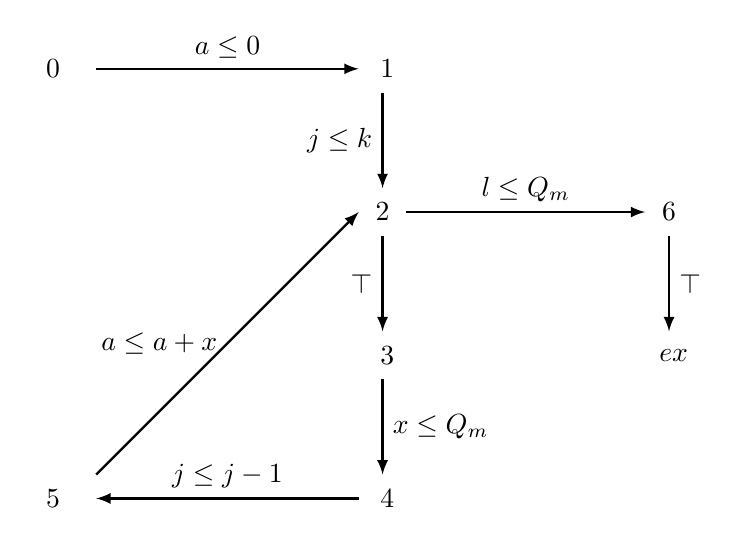
\begin{tikzpicture}[scale=\textwidth/20cm,samples=200]
  \draw[] (-7, 10) circle (0pt) node{{ $0$}};
  \draw[] (0, 10) circle (0pt) node{{ $1$}};
  \draw[] (0, 7) circle (0pt) node{\textbf{$2$}};
  \draw[] (0, 4) circle (0pt) node{{ $3$}};
  \draw[] (0, 1) circle (0pt) node{{ $4$}};
  \draw[] (-7, 1) circle (0pt) node{{ $5$}};
  % Counter Variables
  \draw[] (6, 7) circle (0pt) node {\textbf{$6$}};
  \draw[] (6, 4) circle (0pt) node {{ $ex$}};
  %
  % Control Flow Edges:
  \draw[ thick, -latex] (-6, 10)  -- node [above] {$a \leq 0$}(-0.5, 10);
  \draw[ thick, -latex] (0, 9.5)  -- node [left] {$j \leq k$} (0, 7.5) ;
  \draw[ thick, -latex] (0, 6.5)  -- node [left] {$\top$}  (0, 4.5);
  \draw[ thick, -latex] (0, 3.5)  -- node [right] {$x \leq Q_m$} (0, 1.5) ;
  \draw[ thick, -latex] (-0.5, 1)  -- node [above] {$j \leq j - 1$} (-6, 1) ;
  \draw[ thick, -latex] (-6, 1.5)  -- node [left] {$a \leq a + x$} (-0.5, 7)  ;
  \draw[ thick, -latex] (0.5, 7)  -- node [above] {$l \leq Q_m$}  (5.5, 7);
  \draw[ thick, -latex] (6, 6.5)  -- node [right] {$\top$} (6, 4.5) ;
  \end{tikzpicture}
  \caption{}
    \end{centering}
    \end{subfigure}
    \begin{subfigure}{.45\textwidth}
      \begin{centering}
    %   \todo{abstract-cfg for two round}
    \begin{tikzpicture}[scale=\textwidth/20cm,samples=200]
    \draw[] (-10, 10) circle (0pt) node{{ $0: 1$}};
    \draw[] (0, 10) circle (0pt) node{{ $1: 1$}};
    \draw[] (0, 7) circle (0pt) node{\textbf{$2: k$}};
    \draw[] (0, 4) circle (0pt) node{{ $3: k$}};
    \draw[] (0, 1) circle (0pt) node{{ $4: k$}};
    \draw[] (-10, 1) circle (0pt) node{{ $5: k$}};
    % Counter Variables
    \draw[] (6, 7) circle (0pt) node {\textbf{$6: 1$}};
    \draw[] (6, 4) circle (0pt) node {{ $ex: 1$}};
    %
    % Control Flow Edges:
  \draw[ thick, -latex] (-8, 10)  -- node [above] {$a \leq 0$}(-1.5, 10);
  \draw[ thick, -latex] (0, 9.5)  -- node [left] {$j \leq k$} (0, 7.5) ;
  \draw[ thick, -latex] (0, 6.5)  -- node [left] {$\top$}  (0, 4.5);
  \draw[ thick, -latex] (0, 3.5)  -- node [right] {$x \leq Q_m$} (0, 1.5) ;
  \draw[ thick, -latex] (-1.5, 1)  -- node [above] {$j \leq j - 1$} (-8, 1) ;
  \draw[ thick, -latex] (-8, 1.5)  -- node [left] {$a \leq a + x$} (-1.5, 7)  ;
  \draw[ thick, -latex] (1.5, 7)  -- node [above] {$l \leq Q_m$}  (4.5, 7);
  \draw[ thick, -latex] (6, 6.5)  -- node [right] {$\top$} (6, 4.5) ;
    \end{tikzpicture}
    \caption{}
      \end{centering}
      \end{subfigure}
    \caption{(a) The same $\kw{towRounds(k)}$ program as Figure~\ref{fig:twoRounds_example}
    (b) The abstract control flow graph for $\kw{towRounds(k)}$  (c) The abstract control flow graph with the reachability bound for $\kw{towRounds(k)}$.}
    \vspace{-0.5cm}
    \label{fig:abscfg_tworound}
  \end{figure}
\end{example}

\subsection{Static Data Dependency Analysis}
\label{sec:static-dep}
% \subsection{Analysis Rules/Algorithms of {\ADAPTSYSTEM}}

The new data dependency relation analysis algorithm
is performed on basis of the standard control flow graph.
\highlight{Improved from previous analysis,
this new analysis algorithm combines the reaching definition analysis into the standard data flow analysis.
It designs an improved version of data flow analysis named feasible 
data-flow, estimating a tighter bound on the data dependency relation. 
}
%  of the program, called abstract control flow graph.
In this part, I first show how to generate the standard abstract control flow graph in
Section~\ref{sec:static-cfg}
Then in Section~\ref{sec:static-feasible_flowsto}, 
I present the new feasible 
data-flow analysis
%  reachability-bound analysis algorithm adapted from the newly-designed
% technique in Chapter~\ref{sec:reachability-analysis} 
for estimating the data dependency relation.
Section~\ref{sec:static-dep_compute}
uses the reachability-bound analysis results estimating the dependency quantity
over labeled variables.
%  and
% Section~\ref{sec:static-quantity-edge} uses the same information
% estimating the dependency quantity for the pairs of dependent variables.
In Appendix~\ref{apdx:flowsto_soundness_extend},
this static algorithm is proved as the sound approximation of the variable \emph{may-dependency} relation
in the execution-based analysis in Section~\ref{sec:dynamic-datadep}.
%  before the introduction of  the edge and weight estimation.  

\subsubsection{Standard Control Flow graph}
\label{sec:static-cfg}
% Another operator \mathsf{blocks} 
The standard control flow graph is generated through following steps.
\paragraph*{Vertices Construction}
The vertices of this graph is the set of $c$'s labels , 
\[ 
  \cfgV(c) = labels(c)
\]
%
% Performing a feasible data-flow analysis through the reachable definition algorithm. 
%  By generating set of all the reachable variables at location of label $l$ in the program $c$.
% For every labelled variable $x^l$ in this set, 
% the value assigned to that variable
% in the assignment command associated to that label is reachable at the entry point of  executing the command of label $l$.
\paragraph*{Edges Construction}
The edges set is constructed in following steps.
\\
\textbf{Initial State:}
%
$\cfginit(c) \in \ldom$.
\\
The \emph{initial state} for a program $c$ is the initial label of this program.
This label corresponds to the first labeled command of this program 
when executing this program.
\\
Given a program $c$, its abstract initial state is computed as follows,
%
\[
  \begin{array}{ll}
    \cfginit(\clabel{\assign{x}{\expr}}{}^l)  & = l  \\
    \cfginit(\clabel{\assign{x}{\query(\qexpr)}}{}^l)  & = l \\
    \cfginit(\clabel{\eskip}^{l})  & = l \\
    \cfginit(\eif [b]^l \ethen c_1 \eelse c_2)  & = l \\
    \cfginit(\ewhile [b]^l \edo c)  & = l \\
    \cfginit(c_1 ; c_2)  & = \cfginit(c_1) \\
 \end{array}
 \]
%

\textbf{Final State}: $\cfgfinal(c) \in \mathcal{P}(\ldom)$
The \emph{Final State} of the program $c$, 
$\cfgfinal(c) \in \mathcal{P}(\ldom)$
is a set of labels.
Every label in $\cfgfinal(c)$ corresponds to the exist point of $c$.
\\
Given a program $c$, its final state is computed as follows,
% computes the set of Final State for the command. 
 \[
  \begin{array}{ll}
    \cfgfinal(\clabel{\assign{x}{\expr}}{}^l)  & = \{l\}  \\
     \cfgfinal(\clabel{\assign{x}{\query(\qexpr)}}{}^l)  & = \{l\}  \\
     \cfgfinal(\clabel{\eskip}^{l})  & = \{l\} \\
     \cfgfinal(\eif [b]^l \ethen c_1 \eelse c_2)  & = \cfgfinal(c_1) \cup \cfgfinal(c_2) \\
     \cfgfinal(\ewhile [b]^l \edo c)  & = \{l\} \\
     \cfgfinal(c_1 ; c_2)  & =  \cfgfinal(c_2) 
 \end{array}
 \]

The control flow graph is generated by edges between labels. 
Define $\cfgflow(c): \mathcal{P}(\ldom \times \ldom)$.
%
\[
 \begin{array}{ll}
    \cfgflow(\clabel{\assign{x}{\expr}}{}^l)  & = \emptyset  \\
    \cfgflow(\clabel{\assign{x}{\query(\qexpr)}}{}^l)   & = \emptyset  \\
    \cfgflow(\clabel{\eskip}^{l})  & = \emptyset \\
    \cfgflow(\eif [b]^l \ethen c_1 \eelse c_2) & =  \cfgflow(c_1) \cup \cfgflow(c_2)\cup \{(l, \cfginit(c_1)) , (l, \cfginit(c_2)) \} \\
    \cfgflow(\ewhile [b]^l \edo c)  & =  \cfgflow(c) \cup \{(l, \cfginit(C)) \} \cup \{(l', l)| l' \in \cfgfinal(c) \} \\
    \cfgflow(c_1 ; c_2)  & = \cfgflow(c_1) \cup  \cfgflow(c_2) \cup \{ (l, \cfginit(c_2)) | l \in \cfgfinal(c_1) \} \\
 \end{array}
 \]

The edges for the control flow graph is generated as follows.
Then, I build the edge for $c$'s abstract control flow graph as follows,
\[
  \cfgE(c) = \{(l_1, l_2) | (l_1, l_2) \in \cfgflow(c)\}
  \]

%  I have a pre-processing algorithm to go through the programs and returns the list of labels associating with a loop and whose visiting times need to be analyzed.
%


\paragraph{Control Flow Graph} 
With the vertices $\cfgV(c)$ and edges $\cfgE(c)$ ready, I construct the abstract control flow graph, formally 
% Through a program $c$'s abstract execution trace, its abstract control flow graph is computed 
defined in 
Definition~\ref{def:abs_cfg}.
% Given program $c$ with its abstract control flow $\cfgflow(c)$, the Abstract Control Flow Graph:
% \\
\begin{defn}[Control Flow Graph]
\label{def:cfg_graph}
Given a program $c$, 
with its abstract control flow $\cfgflow(c)$
its abstract control flow graph $\cfgG(c) =(\cfgV(c), \cfgE(c))$ is defined as follows,
\\
% \highlight{
% :
%
% \\
$\cfgE(c) = \{(l_1, dc, l_2) | (l_1, dc, l_2) \in \cfgflow(c)\}$,
\\
$\cfgV(c) = labels(c)$
% }
% \\
% , where the weight of every label to be computed in the next step.
\end{defn}




\subsubsection{Feasible Data-Flow Analysis}
\label{sec:static-feasible_flowsto}
I develop a variant of data flow analysis, called Feasible Data-Flow Generation, which 
considers both the control flow and data flow and
is a sound approximation of the edges in the execution based dependency graph.

% \wq{
\highlight{Improved from previous analysis,
this new analysis algorithm combines the reaching definition analysis on the control flow graph in feasible 
data-flow generation to have a more precise approximation. 
}
% }

% In this step, through 
% % the vertices and edges in 
% $c$'s abstract contrl flow graph $\cfgG(c)$,
%  $\THESYSTEM$ performs a feasible data-flow analysis 
%  using the reachable definition algorithm,
% %  and then Then I generated the set of feasible data-flow between labeled variables based on that.
% and generates the 
% %set of 
% feasible data-flow relation between labeled variables.
% \\
%  By generating set of all the reachable variables at location of label $l$ in the program $c$.
% For every labelled variable $x^l$ in this set, 
% the value assigned to that variable
% in the assignment command associated to that label is reachable at the entry point of  executing the command of label $l$.
% \\
It first defines some operations and then
% In the first step, 
% it 
performs the standard reaching definition analysis given a program $c$, 
on 
% its every label $l$
every label in $\cfgV(c)$.  
% \\
% it performs the standard reaching definition analysis given a program $c$, on its every label $l$.
% \\
% Another operator \mathsf{blocks} 
%
% Performing a feasible data-flow analysis through the reachable definition algorithm. 
%  By generating set of all the reachable variables at location of label $l$ in the program $c$.
% For every labelled variable $x^l$ in this set, 
% the value assigned to that variable
% in the assignment command associated to that label is reachable at the entry point of  executing the command of label $l$.
% \paragraph{Generate CFG}
%  \begin{def}
%   \label{def:init_label}
%   Define $\mathsf{init}$: Command -> label, which returns the initial label of the statement. 
% \[
%  \begin{array}{ll}
%     init([x := e]^{l})  & = l  \\
%      init([x := q(e)]^{l})  & = l \\
%      init([skip]^{l})  & = l \\
%      init([if [b]^l then C_1 else C_2]^{l})  & = l \\
%      init([while [b]^l do C]^{l})  & = l \\
%      init(C_1 ; C_2)  & = init(C_1) \\
%  \end{array}
%  \]
% \end{def}
%   Define $\mathsf{final}$: Command -> Powerset(label), which returns the final labels of the statement. 
%  \[
%  \begin{array}{ll}
%     final([x := e]^{l})  & = \{l\}  \\
%      final([x := q(e)]^{l})  & = \{l\}  \\
%      final([skip]^{l})  & = \{l\} \\
%      final([if [b]^l then C_1 else C_2]^{l})  & = final(C_1) \cup final(C_2) \\
%      final([while [b]^l do C]^{l})  & = \{l\} \footnote{while terminates after b evaluates to false} \\
%      final(C_1 ; C_2)  & =  final(C_2) \\
%  \end{array}
%  \]
% \paragraph*{Blocks and Defs}
%  Define block B to be either the command of the form of assignment, skip, or test of the form of $[b]^{l}$.\\
%  Define $\mathsf{blocks}$ : command -> Powerset(Block)
%  \[
%  \begin{array}{ll}
%     blocks([x := e]^{l})  & = \{[x := e]^{l}\}  \\
%      block([x := q(e)]^{l})  & = \{[x := q(e)]^{l}\}  \\
%      blocks([skip]^{l})  & = \{[skip]^{l}\} \\
%      blocks([if [b]^l then C_1 else C_2]^{l})  & = {[b]^{l}} \cup blocks(C_1) \cup blocks(C_2) \\
%      blocks([while [b]^l do C]^{l})  & = \{[b]^{l}\} \cup blocks(C) \\
%      blocks(C_1 ; C_2)  & = blocks(C_1) \cup  blocks(C_2) \\
%  \end{array}
%  \]
%  Define $\mathsf{labels}$ to get the labels of blocks.
%  \[
%    labels(C) = \{l | [B]^{l} \in blocks(C) \}
%  \]  

% The control flow graph is generated by edges between labels. Define $\mathsf{flow}$: command -> P (label $\times$ label ).

% \[
%  \begin{array}{ll}
%     flow([x := e]^{l})  & = \emptyset  \\
%      flow([x := q(e)]^{l})  & = \emptyset  \\
%      flow([skip]^{l})  & = \emptyset \\
%      flow([if [b]^l then C_1 else C_2)  & =  flow(C_1) \cup flow(C_2)\cup \{(l, init(C_1)) , (l, init(C_2)) \} \\
%      flow([while [b]^l do C)  & =  flow(C) \cup \{(l, init(C)) \} \cup \{(l', l)| l' \in final(C) \} \\
%      flow(C_1 ; C_2)  & = flow(C_1) \cup  flow(C_2) \cup \{ (l,init(C_2)) | l \in final(C_1) \} \\
%  \end{array}
%  \]
 
%  Define block B to be either the command of the form of assignment, skip, or test of the form of $[b]^{l}$.\\
%  Define $\mathsf{blocks}$ : command -> Powerset(Block)
\paragraph*{Blocks and Defs}
The block, 
is either the command of the form of assignment, skip, or a test of the form of $[b]^{l}$, 
% and $block$ of program $c$ is 
denoted by $\mathsf{blocks}(c)$
the set of all the blocks 
in program $c$, where  $\mathsf{blocks}: \cdom \to \mathcal{P}(\cdom \cup \clabel{\bexpr}^{l})$.
Then it generates the set of feasible data-flow between labeled variables with detail in Definition~\ref{def:feasible_flowsto}, 
based on $\live(l, c)$ for every label in a program $c$ and its blocks $\mathsf{blocks}$.
\\
The details are as follows.

The operator $\mathsf{blk} : \cdom \to \mathsf{blocks}$ gives all the blocks in program $c$.
\\
 \[
 \begin{array}{ll}
  \mathsf{blk}(\clabel{\assign{x}{\expr}}{}^l)  & = \{(\clabel{\assign{x}{\expr}}{}^l)\}  \\
  \mathsf{blk}(\clabel{\assign{x}{\query(\qexpr)}}{}^l)  & = \{(\clabel{\assign{x}{\query(\qexpr)}}{}^l)\}  \\
  \mathsf{blk}([\eskip]^{l})  & = \{[\eskip]^{l}\} \\
  \mathsf{blk}(\eif [b]^l \ethen c_1 \eelse c_2)  & = {[b]^{l}} \cup \mathsf{blk}(c_1) \cup \mathsf{blk}(c_2) \\
  \mathsf{blk}(\ewhile [b]^l \edo c)  & = \{[b]^{l}\} \cup \mathsf{blk}(c) \\
  \mathsf{blk}(C_1 ; C_2)  & = \mathsf{blk}(c_1) \cup  \mathsf{blk}(c_2) \\
 \end{array}
 \]
%  $label^{?}$ is label $\cup \{?\}$.\\
%  Define $\mathsf{kill}$: $blocks \to \mathcal{P}(\mathcal{VAR} \times LABEL \cup \{?\})$, which produces the set of labelled variables of assignment destroyed by the block.
\paragraph*{Kills and Gens}
The operator $\mathsf{kill}$: $\mathsf{blocks} \to \mathcal{P}(\mathcal{VAR} \times \ldom \cup \{?\})$ produces the set of labelled variables of assignment destroyed by the block.
 \\
  % Define $\mathsf{gen}$: $blocks \to \mathcal{P}(\mathcal{VAR} \times LABEL \cup \{?\})$, which generates the set of labelled variables generated by the block.
  The operator $\mathsf{gen}$: $\mathsf{blocks} \to \mathcal{P}(\mathcal{VAR} \times \ldom \cup \{?\})$ generates the set of labelled variables generated by the block.
  \\
  % Define $defs(x)(c): \mathcal{VAR} \to LABEL$, gives all the labels where assigns value to variable x in the target program $c$. 
  % The operator  $defs(c): \mathcal{VAR} \to \ldom$ gives all the labels where assigns value to variable in $c$. 
 \[
 \begin{array}{ll}
  \mathsf{kill}(\clabel{\assign{x}{\expr}}{}^l)  & = \{ (x, ?) \} \cup \{ (x, l') | l' \in defs(x) \} \\
  \mathsf{kill}(\clabel{\assign{x}{\query(\qexpr)}}{}^l)  & = \{ (x, ?) \} \cup \{ (x, l') | l' \in defs(x) \}  \\
  \mathsf{kill}([\eskip]^{l})  & = \emptyset \\
  \mathsf{kill}([ [b]^l ]^{l})  & =  \emptyset
 \end{array}
 ~~
  \begin{array}{ll}
    \mathsf{gen}(\clabel{\assign{x}{\expr}}{}^l)  & = \{ (x, l) \}  \\
    \mathsf{gen}(\clabel{\assign{x}{\query(\qexpr)}}{}^l)  & = \{ (x, l) \}  \\
    \mathsf{gen}([\eskip]^{l})  & = \emptyset \\
    \mathsf{gen}([ [b]^l ]^{l})  & =  \emptyset 
 \end{array}
 \]
 The $?$ is a placeholder for the unknown label need to be comptued.
%  Define $in(l)$, $out(l)$: LABEL$ \to \mathcal{VAR} \times LABEL \cup \{?\}$ for every block in program $c$ is computed as follows,
%  \[
%  \begin{array}{lll}
%     in(l)  & = \{ (x, ?) | x^l \in \lvar_c \land  l = \cfginit(c) \}  
%     \cup \{ out(l')|  | (l',\_, l) \in \cfgE \land  l \neq \cfginit(c)\}  \\
%      out(l)  & =  gen(B^{l}) \cup \{ in(l) \setminus kill(B^l)  \} & B^l \in blocks(c)   
%  \end{array}
%  \]
%  computing $in(l)$ and $out(l)$ for every $B^l \in blocks(c) $, and repeating these two step
% until the $in(l)$ and $out(l)$ are stabilized for every $B^l \in blocks(c) $
%  I use $\live_{in}(l,c)$ and $\live_{out}(l, c)$ denote the stabilized results for the command of label $l$ in program $c$. 
%  Define $defs(x)(c): \mathcal{VAR} \to LABEL$, gives all the labels where assigns value to variable x in the target program $c$.
% Define $defs(x)(c): \mathcal{VAR} \to \ldom$, gives all the labels where assigns value to variable x in the target program $c$.
% \\
%  Define $in(l)$, $out(l)$: $ \ldom \to \mathcal{VAR} \times LABEL \cup \{?\}$ for every block in program $c$ is computed as follows,
\paragraph*{In and Out}
The operator  $in(l)$, $out(l)$: $ \ldom \to \mathcal{LV} \cup \{?\}$ for every block in program $c$ is defined as follows,
 \[
 \begin{array}{ll}
    % in(l)  & = \{ (x, ?) | x^l \in \lvar_c \land  l = \cfginit(c) \}  
    in(l)  & = \{ x^{?} | x^l \in \lvar_c \land  l = \cfginit(c) \}  
    \cup \{ out(l')|  | (l',\_, l) \in \cfgE(c) \land  l \neq \cfginit(c)\}  \\
     out(l)  & =  \mathsf{gen}(B^{l}) \cup \{ in(l) \setminus \mathsf{kill}(B^l)  \}  
 \end{array}
 \]
computing $in(l)$ and $out(l)$ for every $B^l \in \mathsf{blk}(c) $, and repeating these two steps
until the $in(l)$ and $out(l)$ are stabilized for every $B^l \in \mathsf{blk}(c) $
%  I use $\live_{in}(l,c)$ and $\live_{out}(l, c)$ denote the stabilized results for the command of label $l$ in program $c$. 
 I use $\live(l,c)$ to represent 
% $\live_{in}(l,c)$ in the other part of the paper.
denote the stabilized result of $in(l)$ at label $l$ in program $c$. 
% The $\live_{in}(l,c)$ and $\live_{out}(l, c)$ is computed by the Standard worklist algorithm. (For simplicity, I use $\live(l,c)$ to represent $\live_{in}(l,c)$ in the other part of the paper.}
\\
% The $\live_{in}(l,c)$ and $\live_{out}(l, c)$ 
\paragraph{Reaching definition computation}
This step generates set of all the reachable variables at location of label $l$ in the program $c$.
The $\live(l, c)$ represent the analysis result, which is the set of 
reachable labeled variables in program $c$ at the location of label $l$.
For every labelled variable $x^l$ in this set, 
the value assigned to that variable
in the assignment command associated to that label is reachable at the entry point of  executing the command of label $l$.

The stabilized $in(l)$ and $out(l)$ for program $c$, as well as $\live(l, c)$,
is computed by the standard worklist algorithm with detail as below. 
% For simplicity, I use $\live(l,c)$ to represent $\live_{in}(l,c)$ in the other part of the paper.
\begin{enumerate}
    \item Initializing in[l]=out[l]=$\emptyset$
    \item Initializing in[entry label] = $\emptyset$
    \item Initializing a work queue, contains all the blocks in $c$
    \item while |W| != 0 \\
         pop l in W\\
          old = out[l]\\
          in(l) =  out(l') where $(l',\_, l) \in \cfgE(c)$\\
           out(l) = $\mathsf{gen}$($b^l$) $\cup$ (in(l) - $\mathsf{kill}$($b^l$) ) where $b^l$ in $\mathsf{blk}(c)$   \\
          if (old != out(l)) W= W $\cup$ \{l'| (l,l') in $(l',\_, l) \in \cfgE(c)$\}\\
          end while
\end{enumerate}
%
% computing $in(l)$ and $out(l)$ for every $B^l \in blocks(c) $, and repeating these two step
% until the $in(l)$ and $out(l)$ are stabilized for every $B^l \in blocks(c) $
%  I use $\live_{in}(l,c)$ and $\live_{out}(l, c)$ denote the stabilized results for the command of label $l$ in program $c$. 
% The $\live_{in}(l,c)$ and $\live_{out}(l, c)$ is computed by the Standard worklist algorithm. (For simplicity, I use $\live(l,c)$ to represent $\live_{in}(l,c)$ in the other part of the paper.
%%
\paragraph{Feasible Data-Flow Generation}
by using the results of Reaching definition analysis results, specifically $\live(l, c)$ for every label in a program $c$, I refine the vertices and edges in the $\cfgG$ graph 
by generating the set of feasible data-flow between labeled variables as follows,
%
%   \[
%  \begin{array}{ll}
%     dcdg([x := e]^{l})  & = \{ (y^i, x^l) | y \in VAR(e) \land (y,i) \in \live_{in}(l) \}  \\
%      dcdg([x := q(e)]^{l})  & = \{ (y^i, x^l) | y \in VAR(e) \land (y,i) \in \live_{in}(l) \}  \\
%      dcdg([skip]^{l})  & = \emptyset \\
%      dcdg([if [b]^l then C_1 else C_2)  & =  dcdg(c_1) \cup dcdg(c_2)\\ & \cup \{(x^i,y^j) | x \in VAR(b) \land (x,i) \in \live_{in}(l) \land ([y = \_]^j) \in blocks(c_1) \} \\
%      &\cup \{(x^i,y^j) | x \in VAR(b) \land (x,i) \in \live_{in}(l) \land ([y = \_]^j) \in blocks(c_2) \} \\
%      dcdg([while [b]^l do c)  & =  dcdg(c) \cup \{(x^i,y^j) | x \in VAR(b) \land (x,i) \in \live_{in}(l) \land ([y = \_]^j) \in blocks(C) \} \\
%      dcdg(c_1 ;c_2)  & = dcdg(c_1) \cup  dcdg(c_2) \\
%  \end{array}
%  \]
%
\begin{defn}[Feasible Data-Flow]
  \label{def:feasible_flowsto}
  Given a program $c$ and two labeled variables $x^i, y^j$  in this program, 
  $\flowsto(x^i, y^j, c)$ is 
    {\footnotesize
    \[
   \begin{array}{ll}
    \flowsto(x^i, y^j, \clabel{\assign{x}{\expr}}{}^l)  & \triangleq (x^i, y^j) \in \{ (y^i, x^l) | y \in \mathsf{FV}(\expr) 
    % \land (y,i) \in \live(l, \clabel{\assign{x}{\expr}}^l) \}  \\
    \land y^i \in \live(l, \clabel{\assign{x}{\expr}}^l) \}  \\
    \flowsto(x^i, y^j, \clabel{\assign{x}{\query(\qexpr)}}{}^l)  & \triangleq (x^i, y^j) \in \{ (y^i, x^l) | y \in \mathsf{FV}(\qexpr) 
    % \land (y,i) \in \live(l,\clabel{\assign{x}{\query(\qexpr)}}^l) \}  \\
    \land y^i \in \live(l,\clabel{\assign{x}{\query(\qexpr)}}^l) \}  \\
    \flowsto(x^i, y^j, [\eskip]^{l})  & = \emptyset \\
    \flowsto(x^i, y^j, \eif ([b]^l, c_1, c_2))  & \triangleq \flowsto(x^i, y^j, c_1) \lor \flowsto(x^i, y^j, c_2) \\ 
        & \lor (x^i, y^j) \in
       \{(x^i,y^j) | x \in \mathsf{FV}(b) \land 
      %  (x,i) 
      x^i \in \live(l, \eif ([b]^l, c_1, c_2)) \land  y^j \in \lvar(c_1) \\
    %   ([y = \_]^j) \in \mathsf{blk}(c_1) \} \\
       &\lor (x^i, y^j) \in \{(x^i,y^j) | x \in \mathsf{FV}(b) \land 
      %  (x,i) 
      x^i\in \live(l, \eif ([b]^l, c_1, c_2))  \land  y^j \in \lvar(c_2) \\
    %   \land ([y = \_]^j) \in \mathsf{blk}(c_2) \} \\
       \flowsto(x^i, y^j, \ewhile [b]^l \edo c_w)  & \triangleq  \flowsto(x^i, y^j, c_w)  \lor
       \\ & 
       (x^i, y^j) \in  \{(x^i,y^j) | x \in \mathsf{FV}(b) \land 
      %  (x,i) 
      x^i \in \live(l,   \ewhile [b]^l \edo c_w) \land  y^j \in \lvar(c_w) \\
    %   ([y = \_]^j) \in \mathsf{blk}(c_w) \} \\
       \flowsto(x^i, y^j, c_1 ;c_2)  & \triangleq \flowsto(x^i, y^j, c_1) \lor \flowsto(x^i, y^j, c_2) \\
   \end{array}
   \]
   }
   \end{defn}
%
This \emph{Feasible Data-Flow} relation is a sound approximation 
of the variable \emph{May-Dependency} relation over labeled variables for every program.
The soundness is proved
in Appendix~\ref{apdx:flowsto_soundness}.
%
\subsubsection{Data Dependency Relation Estimation}
\label{sec:static-dep_compute}
%
For any program $c$ and two labeled variables $x^i, y^j$  in this program, 
$x^i, y^j$  is in the estimated dependency relation if and only if they satisfy
$\flowsto(x^i, y^j, c)$.

As introduce in the third step in Section~\ref{sec:static-overview},
this set is used in Section~\ref{sec:static-adapt} to estimate
the execution-based dependency graph.
As introduced in third step of this analysis framework in Section~\ref{sec:static-overview},
this information will be used in constructing the program-based dependency graph, to estimate the execution-based dependency graph for the program.
For easy understanding,
I reveal the estimated directed edges construction below
% vertex and weight construction of this estimated graph below
and presents the formal definition later. 
% for each vertex in $\progV(c)$,
This estimated directed edges set is defined as a set of triples 
% $\progW(c) \in \mathcal{P}(\mathcal{LV} \times \mathcal{LV} \times EXPR(\constdom))$ 
$\progE(c) \in \mathcal{P}(\mathcal{LV} \times \mathcal{A}_{\lin} \times \mathcal{LV})$,
Each directed edge is defined between vertices $({x}_1^{i}, w_1)$  
and $({x}_2^{j}, w_2)$ 
where ${x}_1^{i}, {x}_2^{j} \in \lvar(c)$, and they are in the estimated dependency relation
% is the set of pairs 
% The weight for each vertex in $\progV(c)$ is computed 
% indicating a directed edge from the first vertex to the second one in each pair
as follows,
\highlight{
  \[
    \progE^0(c) \triangleq 
    \left\{ 
    ({x}_1^{i}, w, {x}_2^{j}) \in \mathcal{LV} \times 
    \mathcal{A}_{\kw{in}} \times \mathcal{LV}
    ~ \middle\vert ~
    \begin{array}{l}
      {x}_1^{i}, {x}_2^{j} \in \lvar(c)
    \land
      % \\
      \exists n \in \mathbb{N}, z_1^{r_1}, \cdots, z_n^{r_n} \in \lvar_{{c}} \sthat
      n \geq 0 \land
      \\
      \flowsto(x^i,  z_1^{r_1}, c) 
      \land \cdots \land \flowsto(z_n^{r_n}, y^j, c) 
    \end{array}
    \right\}
    \]
}
The weight $w$ for every edge in this definition is a placeholder.
It will be computed in Section~\ref{sec:static-quantity}.
We prove that this estimated directed edge set $\progE(c)$ is a sound approximation of the 
edge set in $c$'s Execution-Based Dependency Graph 
in Appendix~\ref{apdx:adapt_soundness}.

% \paragraph*{Edges Estimation}
% Then I define the estimated directed edges
% % for each vertex in $\progV(c)$,
% between vertices in $\progV(c)$,
% as a set of pairs 
% % $\progW(c) \in \mathcal{P}(\mathcal{LV} \times \mathcal{LV} \times EXPR(\constdom))$ 
% $\progE(c) \in \mathcal{P}(\in \mathcal{LV} \times \mathcal{LV})$
% % is the set of pairs 
% % The weight for each vertex in $\progV(c)$ is computed 
% indicating a directed edge from the first vertex to the second one in each pair
% as follows,
% \highlight{
%   \[
%     \progE(c) \triangleq 
%     \left\{ 
%     ({x}_1^{i}, {x}_2^{j}) \in \mathcal{LV} \times \mathcal{LV}
%     ~ \middle\vert ~
%     \begin{array}{l}
%       {x}_1^{i}, {x}_2^{j} \in \progV(c)
%     \land
%       % \\
%       \exists n \in \mathbb{N}, z_1^{r_1}, \cdots, z_n^{r_n} \in \lvar_{{c}} \sthat  
%       n \geq 0 \land
%       \\
%       \flowsto(x^i,  z_1^{r_1}, c) 
%       \land \cdots \land \flowsto(z_n^{r_n}, y^j, c) 
%     \end{array}
%     \right\}
%     \]
% }
% This estimated directed edge set $\progE(c)$ is a sound approximation of the 
% edge set in $c$'s execution-based dependency graph, which is proved 
% in Appendix~\ref{apdx:adapt_soundness}.
%  \begin{defn}[Feasible Data-Flow]
%   \label{def:feasible_flowsto}
%     {\footnotesize
%     \[
%    \begin{array}{ll}
%       dcdg(\clabel{\assign{x}{\expr}}{}^l)  & = \{ (y^i, x^l) | y \in FV(e) \land (y,i) \in \live_{in}(l, \clabel{\assign{x}{\expr}}^l) \}  \\
%        dcdg(\clabel{\assign{x}{\query(\qexpr)}}{}^l)  & = \{ (y^i, x^l) | y \in FV(e) \land (y,i) \in \live_{in}(l,\clabel{\assign{x}{\query(\qexpr)}}^l) \}  \\
%        dcdg([\eskip]^{l})  & = \emptyset \\
%        dcdg([\eif [b]^l \ethen c_1 \eelse c_2)  & =  dcdg(c_1) \cup dcdg(c_2)\\ & \cup 
%        \{(x^i,y^j) | x \in FV(b) \land (x,i) \in \live_{in}(l) \land ([y = \_]^j) \in blocks(c_1) \} \\
%        &\cup \{(x^i,y^j) | x \in FV(b) \land (x,i) \in \live_{in}(l) \land ([y = \_]^j) \in blocks(c_2) \} \\
%        dcdg([\ewhile [b]^l \edo c)  & =  dcdg(c) \cup \{(x^i,y^j) | x \in FV(b) \land (x,i) \in \live_{in}(l) \land ([y = \_]^j) \in blocks(C) \} \\
%        dcdg(c_1 ;c_2)  & = dcdg(c_1) \cup  dcdg(c_2) \\
%    \end{array}
%    \]
%    }
%    \end{defn}
%    For any two labeled variables $x^i, y^j$ in a program $c$, 
%   %  it is easy to see that there is a one-on-one correspondence between 
%   %  $\flowsto$ relation of the two variables, and the $dcdg$ analysis result on $c$.
%   I use $\flowsto()$ denote if they have a feasible data-flow relation in Definition~\ref{def:flowsto}.
%    \begin{defn}[Feasible Data-Flow ($\flowsto$)]
%    \label{def:flowsto}
%    \[
%    \forall c \in \cdom, x^i, y^j \in \lvar_c \sthat  
%    \flowsto(x^i, y^j, c) \iff (x^i, y^j) \in dcdg(c)
%    \]
%    \end{defn}
  %  This soundness is proved in Proof~\ref{pf:rd_soundness} in Appendix~\ref{apdx:rd_soundness}.
  %  For any two labeled variables in a program $c$, it is easy to see that there is a one-on-one correspondence between 
  %  $\flowsto$ relation of the two variables, and the $dcdg$ analysis result on $c$.
  %  \begin{thm}[Soundness of the Feasible Data-Flow Analysis]
  %  \label{thm:rd_soundness}
  %  \[
  %  \forall c \in \cdom, x^i, y^j \in \lvar_c \sthat  
  %  \flowsto(x^i, y^j, c) \iff (x^i, y^j) \in dcdg(c)
  %  \]
  %  \end{thm}
  %  This soundness is proved in Proof~\ref{pf:rd_soundness} in Appendix~\ref{apdx:rd_soundness}.
  \paragraph*{Example}
% Still looking at the Figure~\ref{fig:adapfun_tworound}(c), 
% and taking the edge $(l^6, a^5)$ for example.
% By $\flowsto(l^6, a^5, c)$, I can see $a$ is used directly in the query expression $\chi[k]*a$,
% in the assignment command $\clabel{\assign{l}{\query(\chi[k]*a)}}^l$,
% i.e., $a \in FV(\chi[k]*a)$.
% Also, from the Reaching definition analysis, I know $a^5 \in \live(6, two-round)$.
% Then I have $\flowsto(l^6, a^5, c)$ and construct the edge $(l^6, a^5)$.
% And same way for constructing the rest edges.
%
The edge $(l^6, a^5)$ in Figure~\ref{fig:twoRounds_example}(c) is constructed by this definition.
% and take  for example.
By $\flowsto(l^6, a^5, c)$, I can see $a$ is used directly in the query expression $\chi[k]*a$,
in the assignment command $\clabel{\assign{l}{\query(\chi[k]*a)}}^l$,
i.e., $a \in FV(\chi[k]*a)$.
Also, from the reaching definition analysis, I know $a^5 \in \live(6, \kw{twoRounds(k)})$.
Then I have $\flowsto(l^6, a^5, c)$ and construct the edge $(l^6, a^5)$.
And the same way for constructing the rest edges. Also, the edge $(x^3,j^5)$ in the same graph represents the control flow, 
caught by the $\flowsto$ relation.
% Still looking at the Figure~3(c) in main paper, 
% and taking the edge $(l^6, a^5)$ for example.
% By $\flowsto(l^6, a^5, c)$, I can see $a$ is used directly in the query expression $\chi[k]*a$,
% in the assignment command $\clabel{\assign{l}{\query(\chi[k]*a)}}^l$,
% i.e., $a \in FV(\chi[k]*a)$.
% Also, from the Reaching definition analysis, I know $a^5 \in \live(6, two-round)$.
% Then I have $\flowsto(l^6, a^5, c)$ and construct the edge $(l^6, a^5)$.
% And same way for constructing the rest edges. Also, the edge $(x^3,j^5)$ in the same graph represents the control flow, caught by our $\flowsto$ relation.
%
  \subsubsection{Improvements Analysis}
  \label{sec:static-dep-improvements}
  \highlight{
    This new data dependency estimation algorithm is more precise and efficient than previous static analysis.
% language and operational semantics design improves the expressiveness, efficiency, and the accuracy to a large extend.
% \todo{Add details}
\begin{itemize}
  %   \item \textbf{Improvements on Expressiveness}
  %   \\
  % This language is extended over the standard while language. 
  % In this sense, it supports all the general data analysis.
  \item \textbf{Improvements on Efficiency}
  \\
  New analysis architecture does not rewrite the program into SSA version.
\\
  New analysis technique does not pre-collect the variables generated during the program.
\\
  New analysis technique does unfold the while loop and perform analysis for each iteration of the loop, 
  instead, it only performs the analysis on the while body once.
  \\
In the three senses above, the efficiency is improved significantly.
  \item \textbf{Improvements on Accuracy}
  Comparing to previous dependency estimation method,
  new analysis technique uses the reachable definition algorithm.
  This algorithm improves the accuracy 
  on the approximating the data dependency relation.
  Let us see a simple example, a program $ [x = 0]^{1}; [x=2]^{2};  [y = x+1]^{3}$. 
The standard data flow analysis 
tells us that both the labeled variable $x^{1}$ and $x${2} may flow to $y^{3}$, which will result in an unnecessary edge ($x^{1}, y^{3}$). The result of reaching definition 
can help us eliminate this kind of edge by telling us, at line $3$, only variable $x^{2}$ is reachable. 
  \end{itemize}
  }

\subsection{Static Data Dependency Quantity Analysis}
\label{sec:static-quantity}

In order to estimate weight for every vertex in the program-based dependency graph,
we perform the symbolic reachability bound analysis on the abstract control flow graph and add weight as shown in Figure~\ref{fig:abscfg_tworound}(c). 
% This because
% the vertices in the two graph share the same unique label, the line number.
% We would like to generate the closure of every edge, which is an equality relation between variables.  Solving this closure gives us the reachability bound for this edge. With all the bound for all the edges in the abstract control flow graph, we can calculate the weight for every vertex in this graph. For example, we show the closure generated for the edge $(4, j < j - 1, 5)$, 
% $\absclr(4, 5) = \varinvar(j)$. The invariant for variable $j$, $\varinvar(j)$ used here is 
% $\varinvar(j) = k * \absclr(1, 2)$, which is generated by all the difference constraints involving $j$ in the graph. Notice the $k$ in $\varinvar(j)$ comes from considering both difference constraint $j<=k$ from edge (1,2) and $j<=j-1$ from (4,5), which intuitively reflects the while loop whose counter is set to $k$ at the beginning and decreases by 1 at each iteration.
% We first generate the invariant for every variable showing up in the difference constraint and not user defined. For example, in the Figure~\ref{def:abscfg_tworound}(b), there are three variables $a$, $x$, $j$ that we will generate invariant for. We show the invariant for the counter $k$, which is $j = k$. 
% $\absclr(1, 2) = 1$
% \\
% => 
% $\absclr(4, 5) = k$
% using the difference constraint on the edges for all 
% through the edges in $\absG(c)$, which correspond to $c$'s abstract transition between labels.
% We infer the invariant for every variable, and compute the transition closure for every abstract transition. By solving the closure
% with the invariants of variables involved in this closure for every transition, we compute
% the symbolic reachability bound of every commands corresponding to this transition. Specifically, this analysis can be performed in four steps:
%  Variable Modification Tracking, Local Bounds Computation,
% Invariant Inference and Closure Generation, and Reachability Bound Computation,
% 
% We present the details of invariant, closure generation, and reachability bound computation as follows.
% with details as follows.
% \\
% %
% 1.  Variable Modification Tracking: collecting the dc for where each variable is increased, decreased and reset: 
% \\
% 2. Local Bounds Computation: 
% \\
% 3. Invariant Inference and Closure Generation
% \\
% 4. Reachability Bound Computation,
% %
% \paragraph*{Variable Modification Tracking}
% Identify the abstract events where each variable is increased, decreased and reset:
% \\
% $\inc: \mathcal{VAR} \to \mathcal{P}(\absevent) $
% the set of the abstract events where the variable increase.
% \\
% $\inc(x) = \{(\absevent, c) | \absevent = (l, l', x' \leq x + v)\}$
% \\
% $\reset: \mathcal{VAR} \to \mathcal{P}(\absevent) $
% The set of the abstract events where the variable is reset.
% \\
% $\dec: \mathcal{VAR} \to \mathcal{P}(\absevent) $
% The set of abstract events where the variable decrease.
% % \\
% % $\dec(x) = \{(\absevent, c) | \absevent = (l, l', x' \leq x - v)\}$
% \\
% $Incr(v) \triangleq \sum\limits_{(\absevent, c) \in \inc(v)}\{\absclr(\absevent) \times v\}$
% %
% \paragraph*{Local Bounds}
% Given a program $c$ with its abstract control flow graph 
% $\absG(c) = (\absV, \absE)$
% \\
% Local Bounds Computation:
% $\locbound: \absevent \to \mathcal{VAR} \cup \constdom$.
% %
% \[ 
% \begin{array}{ll}
%   \locbound(\absevent) \triangleq 1 
%   & \absevent \notin SCC(\absG(c))
%   \\
%   \locbound(\absevent) \triangleq (x, v) 
%   & \absevent \in SCC(\absG(c)) \land \absevent \in \dec(x) \land  \absevent = (\_, \_ , x' \leq x - v) \\
%   \locbound(\absevent) \triangleq (x, \max(\dec(x))) 
%   & \absevent \in SCC(\absG(c)) \land 
%   \absevent  \notin \bigcup_{x \in \mathcal{VAR}} \dec(x)
%   \land \absevent \notin SCC(\absG(c) \setminus \dec(x)) 
% \end{array}
%   \]
%   The first case is straightforward. Since variable's visiting time outside of any while loop is at most 1, we do not need to analyze the visiting times of every node in the graph from phase 1.
%   The second and third step is guaranteed by the \emph{Discussion on Soundness} in Section 4 of \cite{sinn2017complexity}.
%   Then soundness proof is in Lemma~\ref{lem:local_bound_sound} in appendix~\ref{apdx:reachability_soundness}.
% %
% \paragraph*{Invariant Inference and Closure Generation }
% Then, computing the bound invariants for variables and the transition closures for abstract events:
% \\ 
% $ \varinvar: \mathcal{VAR} \cup \constdom \to EXPR(\constdom)$
% \\
% $\absclr: \absevent \to EXPR(\constdom)$
% \\
% Then, the symbolic invariant for each variable 
% as well as the symbolic transition closure for each transition is calculated as follows:
% \[ 
% \begin{array}{lll}
%   \varinvar(x) & \triangleq c & c \in \constdom \\
%   \varinvar(x) & \triangleq Incr(v) + \max(\{\varinvar(a) + c | (t, a, c) \in \reset(x)\}) & c \notin \constdom
% \end{array}
% \]
% %
% \begin{defn}
%   \label{def:transition_closure_base}
% \[ 
% \begin{array}{lll}
%   \absclr(\absevent) 
%   & \triangleq x / v & \\ 
%   & \locbound(\absevent) = (x, v) \in \constdom \times \mathbb{N} & \\
%   \absclr(\absevent) 
%   & \triangleq (Incr(x) + 
%   \sum\limits_{(\absevent', y, v') \in \reset(x)}
%   \absclr(\absevent') \times \max(\varinvar(y) + v', 0) ) / v & \\
%   & \locbound(\absevent) = (x, v) \land x \notin \constdom & 
% \end{array}
%   \]
% \end{defn}
% %
% \paragraph*{Improved Variable Modification Tracking}
% Instead of just identifying the abstract events where each variable is reset,
% this improvement identifies the chain of the events where a given variable is reset by the 
% variables of the abstract events through the chain.
% \\
% $\resetchain: \mathcal{VAR} \to \mathcal{P}(\mathcal{P}(\absevent)) $
% The set of the chain of abstract events where the variable is reset through the chain.
% % \\
% % $Incr(v) \triangleq \sum\limits_{(\absevent, c) \in \inc(v)}\{\absclr(\absevent) \times v\}$
% %
% \paragraph*{Improved Invariant Inference and Closure Generation}
% Then, computing the bound invariants for variables and the transition closures for abstract events:
% \\ 
% $ \varinvar: \mathcal{VAR} \cup \constdom \to EXPR(\constdom)$
% \\
% $\absclr: \absevent \to EXPR(\constdom)$
% \\
% Then, the symbolic invariant for each variable 
% as well as the symbolic transition closure for each transition is calculated as follows:
% \[ 
% \begin{array}{lll}
%   \varinvar(x) & \triangleq c & c \in \constdom \\
%   \varinvar(x) & \triangleq Incr(v) + \max(\{\varinvar(a) + c | (t, a, c) \in \reset(x)\}) & c \notin \constdom
% \end{array}
% \]
% %
% \begin{defn}
%   \label{def:transition_closure}
% \[ 
% \begin{array}{lll}
%   \absclr(\absevent) 
%   & \triangleq x / v & \\ 
%   & \locbound(\absevent) = (x, v) \in \constdom \times \mathbb{N} & \\
%   \absclr(\absevent) 
%   & \triangleq \Big(
%     \sum\limits_{y \in \{ y ~|~ 
%     ch \in \resetchain(x), (l_1, x, y, v, l_2) \in ch \} } Incr(x) & \\
%     & \quad + 
%   \sum\limits_{ch \in \resetchain(x)}
%   \big( \min\limits_{\absevent' \in ch}({\absclr(\absevent')}) \times 
%   \max(\varinvar(y) + \sum\limits_{(l_1, x, y, v, l_2) \in ch } v, 0)\big) \Big) / v & \\
%   & \locbound(\absevent) = (x, v) \land x \notin \constdom & 
% \end{array}
%   \]
% \end{defn}
  %
% \paragraph*{Adding the Reachability Bounds for Every Vertex in the Data-Control Flow Graph}
% Updating the weight of every vertex in the $\progG(c) = (\progV, \progE, \progW, \progF)$ for program $c$ generated from phase 1. 
% For every $x^l \in \progV$, find the abstract event $\absevent \in \absflow(c)$ of the form $(l, \_, \_)$, updating the $\progW(x^l) $ by the transition closure of this event.
% \\
% \paragraph*{Reachability Bound Computation}
% With all the closures for all the edges of the abstract control flow graph, we can solve them to obtains the reachability bound of every edges. We decide the weight for every vertex in the abstract control flow graph by using the bound of the edges which head out from this vertex, by taking the max of the bound from these involving edges. For instance,   
% By the constraint on the edge $(4, j \leq j - 1, 5)$, we get bound $k$ for this edge.
% Then, we assign vertex $4$ by reachability bound $k$, as in Figure~\ref{fig:abscfg_tworound}(c). 
% Another interesting vertex is $2$, which has more than one edge heading out from it, $(2, \top, 3)$ and $(2,\top, 6)$. For the weight for vertex $2$, we choose the max between the bound $k$ from $(2,\top, 3)$ and $1$ from $(2,\top, 6)$.
% we first infer its local bound as variable $j$.
% Then by solving the invariant for variable $j$,
% we infer the value bound for $j$, which is $k$.
% Then the reachability bound for this abstract transition, (i.e., edge $4, j \leq j - 1, 5$) 
% is computed as $k$ as well through Definition~\ref{def:abs_trace}.
% \\
% $
% \progW(x^l) 
%   \triangleq \absclr(\absevent)
% $
% Through the transition closure computed above, 
% The weight of every label in 
% % Then we update 
% the program $c$'s abstract control flow graph,
% $\absG(c) =(\absV, \absE, \absW)$
% is 
% computed as the maximum over all the abstract events $\absevent \in \absE$ heading out from this vertex, formally as follows.
% % by annotating each vertex with a symbolic weight. 
% % This weight corresponds to 
% %reachability bounds of
% \\
% $\absW 
% \triangleq \left\{ (l, w) \in \mathbb{N} \times EXPR(\constdom) | w = \max\limits_{\absevent = (l, \_, \_)} \{ \absclr(\absevent)\} \right\}$.
% % \\
% \paragraph*{Example}
% Still looking at the two-round example as in Figure~\ref{fig:abscfg_tworound}(b) where 
% each label $l$ is added with a weight by $absW$.
% This weight represents the  maximum reaching times of this location $l$, in the other word,
% the estimated maximum visiting times of the command labeled with $l$.
% For example, looking at the vertex $1$,
% by analysis steps, since it isn't in any SCC, it's estimated reachability bound is computed as $1$.
% However, for the vertex $4$ which is involved in an SCC, the reachability bound is inferred in another way.
% By the constraint on the edge $4, j \leq j - 1, 5$,
% we first infer its local bound as variable $j$.
% Then by solving the invariant for variable $j$,
% we infer the value bound for $j$, which is $k$.
% Then the reachability bound for this abstract transition, (i.e., edge $4, j \leq j - 1, 5$) 
% is computed as $k$ as well through Definition~\ref{def:abs_trace}.
% In this abstract control flow graph, every vertex is a label,
% corresponding to a label command in the program.
% Each directed 
% edge represents an abstract transition 
% between two control locations, 
% i.e., the labels of two commands (we call the labels also control location and they refer to the same thing), 
% where the second labeled command will be executed after execution of the command with first label.
% For example, the edge $0, a \leq 0, 1$ on the top, represents,
% from location $0$, the command 
% $\clabel{\assign{a}{0}}^0$ is executed with next continuation location $1$,
% where the 
% command $\clabel{\assign{j}{k}}^1$ will be executed next.
% The constraint $a \leq 0$ is generated by abstracting from the assignment command $\assign{a}{0}$,
% representing that value of $a$ is less than or equals to $0$ after 
% location $0$ before executing command at line $1$.
%
% The same way for the rest weights' computation.
We use $\absW(c)$ for the computed weights, 
a set of pairs 
$(l, w)$ where 
$w$ is the weight 
for label $l$ from the abstract control flow graph of $c$.
% The weight $w$ for each label $l$ 
$w$ is an arithmetic  expression over $\mathbb{N}$ and
input variables, denoted by $\mathcal{A}_{in}$.
This analysis is  inspired from the program complexity analysis method in \cite{sinn2017complexity}.
The detail of our symbolic reachability bound analysis which uses the difference constraint of the abstract control flow graph can be found in the appendix.
%
%
% \paragraph{Vertex Weight Computation}
% The weight for each vertex in $\progV(c)$ is computed as follows,
Then we compute the weight for each vertex in $\progV(c)$,
as a set of pairs $(x^l, w) \in \ldom \times \mathcal{A}_{in}$
% $\progW(c) \in \mathcal{P}(\mathcal{LV} \times \mathcal{LV} \times EXPR(\constdom))$ 
% is the set of pairs 
% The weight for each vertex in $\progV(c)$ is computed 
mapping each $x^l \in \progV(c)$ to an arithmetic  expression over $\mathbb{N}$ and
input variables. 
Because
the vertices in the two graph share the same unique label, the line number of the same command,
we define $\progW(c)$
% denoted by $\mathcal{A}_{in}$
as follows,
{
% :
% \\
 \[\progW(c) \triangleq
%   \left
  \{ (x^l, w)
\mid
x^l \in \progV(c) \land (l, w) \in \absW(c)
% \right
\}.
\]
}
%
We prove that this 
% symbolic expression is the upper bound for $x^l$'s 
arithmetic expression for $x^l \in \progV(c)$ is a sound upper bound of 
the maximum visiting times of $x^l$ over all execution traces of $c$, with the full proof in the appendix.
  \begin{thm}[Soundness of the Reachability Bounds Estimation]
    \label{thm:addweight_soundness}
  Given a program ${c}$ with its estimated weight $\progW(c)$
%   program-based dependency graph 
%   $\progG = (\progV, \progE, \progW, \progF)$,
  % $\traceG = (\traceV, \traceE, \traceW, \traceF)$, 
  we have:
    %
  \[
  \forall (x^l, w) \in \progW, \vtrace_0 \in \mathcal{T}_0(c), \trace \in \mathcal{T},
  v \in \mathbb{N}
   \st 
  % \max \left\{ 
    % \vcounter(\vtrace') l ~ \middle\vert~
  % \forall \vtrace, \trace' \in \mathcal{T} \st 
  \config{{c}, \trace_0} \to^{*} \config{\eskip, \trace_0 \tracecat\vtrace} 
  \land 
  \config{\vtrace_0, w} \earrow v
  \implies
  % \right\} 
  \vcounter(\vtrace, l) \leq v
  \]
  \end{thm}
% appendix~\ref{apdx:reachability_soundness}. 
%
\paragraph*{Example} 
As in
Figure~\ref{fig:twoRounds_example}(c),
the weight for $a^5$ is $k$. which is a sound estimated weight.
% in program-based dependency Graph as $k$ as well.
For any initial $\trace_0 \in \mathcal{T}_0(c)$, we know $\config{\trace_0, k} \earrow \env(\trace_0) k$ and
the weight $w_k$ for vertex $a^5$ from Figrue~\ref{fig:overview-example}(b)
$w_k(\trace_0) = \env(\trace_0) k$. 
%
In the same way, the weights for all the other vertices are sound.
% for the rest weights' computation.

\subsection{Adaptivity Estimation through Dependency Graph}
\label{sec:static-adapt}
% \subsection{Program-Based Data Dependency Graph Generation}
% %  Weighted Data Dependency Graph Generation}
%  \label{sec:alg_graphgen}
 %
%    Each directed edge represents an abstract transition 
%    between two control locations, i.e., the labels of two commands (we call the labels also control location and they refer to the same thing in the follows), 
%    where the second labeled command will be executed after execution of the command with first label.
%    The abstract transition contains a set of difference constraints for variables, generated by abstracting the command of the first label.
%   \item Computing 
%   % I get the reachability bound for each command.
%   the symbolic reachability bound for each command,
%   % the value bound invariant for each variable in the event and 
%   by inferring the value bound invariant for each variable 
%   % the event transition closure over the abstract control flow graph,
%   and the transition closure for every abstract transition through the constraints over the abstract control flow graph.
%   % \\
%   % Through this graph and constraint for every transition, I infer the  invariant for every variable,
%   % and compute the transition closure for every abstract transition.
%   % By solving the closure with the invariants of variables involved in this closure for every transition, 
%   % I compute the symbolic reachability bound of every commands corresponding to 
% %     % this transition.
% %     \item Performing a feasible data-flow analysis from the reachable definition algorithm. 
% % %  By generating set of all the reachable variables at location of label $l$ in the program $c$.
% % and generating the set of all the reachable variables for every program location.
% % For every labelled variable $x^l$ in this set, 
% % the value assigned to that variable
% % in the assignment command associated to that label is reachable at the entry point of  executing the command of label $l$.
% % \item Refining the abstract control flow graph into a weighted-data dependency graph, 
% % by annotating each vertex with reachability bounds and 
% % removing unfeasible edges and redundant edges and vertices.
% % adding edges between
% %     variables having data-flow relations, and
% % removing the edges between locations where the variables associated to that labeled command isn't reachable from the second location.
% % \\
% % first annotate each vertex of label $l$ with the variable 
% % assigned in that labeled command, and remove the rest doesn't correspond to an assignment command.
% % Then 
% % add direct edge between two labeled variables,
% % where the first variable 
% % is directly used in the assignment expression to the second variable, by restricting 
% % the first labeled variable is reachable at the the second label.
% %
% \item Computing the adaptivity through this weighted data dependency graph,
%   by finding a finite walk on this weighted graph, 
% traversing the maximum times of query variables, by restricting the visiting time of every vertex on this walk to its weight.
% The maximum number of vertices corresponding to a query variables visited on this walk is the estimated upper bound, for program's adaptivity.

%    In this step, $\THESYSTEM$ refines the abstract control flow graph into the program-based weighted-data dependency graph, 
% by annotating each vertex with reachability bounds and 
% removing unfeasible edges and redundant edges and vertices,
% % This graph is used 
% for approximating the trace-based weight-data dependency graph.
% \\
% Specifically, I first annotate each vertex of label $l$ with the variable 
% assigned in that labeled command, and remove the rest doesn't correspond to an assignment command.
% Then 
% add direct edge between two labeled variables,
% where the first variable 
% is directly used in the assignment expression to the second variable, by restricting 
% the first labeled variable is reachable at the second label.
% % \\
% The formal definition is as follows.
Based on the variable \emph{may-dependency} relation in Section~\ref{sec:dynamic-datadep} and 
the dependency quantity analysis in Section~\ref{sec:dynamic-reachability}.
% gives us the edges, 
I firstly define the execution-based dependency graph, then formalize the \emph{adaptivity} in this section.

\subsubsection{Program-Based Data Dependency Graph Generation}
%  Weighted Data Dependency Graph Generation}
 \label{sec:alg_graphgen}
\todo{Remove:
 To build the graph, we firstly estimate the vertices and query annotations straightforwardly as follows.
\paragraph{Vertices Estimation and Query Annotation Estimation}
\label{sec:alg_vertexgen}
The vertices in the static analysis dependency graph are actually identical as the  Execution-Based Dependency Graph, which are assigned variables in the program annotated with the unique label(line number). These vertices are collected by statically scanning the program, like what I do for vertices of its Execution-Based Dependency Graph. The vertices are defined formally as follows.
%
  \highlight{
\[
    \progV(c) \triangleq \left\{ 
  x^l \in \mathcal{LV} 
  ~ \middle\vert ~
  x^l \in \lvar_{c}
  \right\}
  \]
  }
  %
%
The static scanning of the programs also tells us whether one vertice(assigned variable) is assigned by a query request.  I have similar definition when defining the Execution-Based Dependency Graph, 
a set of pairs $\progF(c) \in \mathcal{P}(\mathcal{LV} \times \{0, 1\} )$ 
% is the set of pairs 
% The weight for each vertex in $\progV(c)$ is computed 
mapping each $x^l \in \progV(c)$ to a flag, either $0$ or $1$, where $1$  means $x^{l}$ is a member of $ \qvar_{c}$, a set of those variables assigned with query requests,
and $0$ means $x^{l}$ not in this set. It is defined formally below.
\[\progF(c) =\left\{(x^l, n)  \in  \mathcal{LV} \times \{0, 1\} 
~ \middle\vert ~
x^l \in \lvar_{c},
n = 1 \iff x^l \in \qvar_{c} \land n = 0 \iff  x^l \not\in \qvar_{c} .
\right\}\]
Then, I build the estimated data dependency graph based on the above program static analysis as follows:
\\
\highlight{
\[
  \progG(c) = (\progV(c), \progE(c), \progW(c), \progF(c))
  \]
}
with $\progV(c), \progE(c), \progW(c)$ and $ \progF(c)$ as computed in each steps above.
% and $\progF(c) =\left\{(x^l, n)  \in  \mathcal{LV} \times \{0, 1\} 
% ~ \middle\vert ~
% x^l \in \lvar_{c},
% n = 1 \iff x^l \in \qvar_{c} \land n = 0 \iff  x^l \in \qvar_{c} .
% \right\} $,
This program-based graph program-based graph has a similar topology structure as 
% the one
% of 
the Execution-Based Dependency Graph. It has the same
vertices and query annotations, but approximated edges and weights.  
% The algorithm computation is 
It is formally defined in Definition~\ref{def:prog_graph}.
% Through the reachable definition set on every label,
% I remove the edges between labels where the variables associated to that labeled command isn't reachable from the second location.
%\absG(c) =(\absV, \absE, \absW)
\begin{defn}
[Program-Based Dependency Graph]
\label{def:prog_graph}
% [Program-Based Weighted Data Dependency Graph Generation Algorithm]
% \label{def:analyz_dcfg}
Given a program $c$, with its abstract weighted control flow graph $\absG(c) = (\absV, \absE, \absW)$ and 
feasible data flow relation $\flowsto(x^i, y^j, c)$ for every $x^i, y^j \in \lvar_c$, its Program-Based Weighted Data Dependency Graph
$\progG(c) = (\progV, \progE, \progW, \progF)$,
is generated as follows,
% \\
% \highlight{
% $\progV =\{x^l | x^l \in \lvar_c\} $
% \\
% $\progE = \{(y^i, x^l) | (y^i, x^l)  \in dcdg(c) \}$
% \\
% $\progW = \{(x^l, w ) | (l, w ) \in \absW \land x^l \in \lvar_c\}$
% \\
% $\progF = \{(l, q) \in \mathcal{L} \times \{0, 1\}| q = 1 \iff l \in \qvar_c, q = 0 \iff l \notin \qvar_c \}$.
% }
% \end{defn}
% \begin{defn}
% [Program-Based Dependency Graph].
% \label{def:prog_graph}
%   % \\
% Given a program ${c}$
% its program-based graph 
% $\progG({c}) = (\vertxs, \edges, \weights, \qflag)$ is defined as:
{\footnotesize
\[
\begin{array}{rlcl}
\text{Vertices} &
\progV & := & \left\{ 
x^l \in \mathcal{LV} 
~ \middle\vert ~
x^l \in \lvar_{c}
\right\}
\\
\text{Directed Edges} &
\progE & := & 
\left\{ 
({x}_1^{i}, {x}_2^{j}) \in \mathcal{LV} \times \mathcal{LV}
~ \middle\vert ~
\begin{array}{l}
{x}_1^{i}, {x}_2^{j} \in \vertxs
\land
% \\
\exists n \in \mathbb{N}, z_1^{r_1}, \cdots, z_n^{r_n} \in \lvar_{{c}} \sthat  
n \geq 0 \land
\\
\flowsto(x^i,  z_1^{r_1}, c) 
\land \cdots \land \flowsto(z_n^{r_n}, y^j, c) 
\end{array}
\right\}
\\
\text{Weights} &
\progW & := &
% \bigcup
% \begin{array}{l}
\left\{ (x^l, w) \in  \mathcal{LV} \times \mathcal{A}_{in}
\mid
x^l \in \lvar_{{c}} \land (l, w) \in \absW(c)
\right\}
% \end{array} 
\\
\text{Query Annotation} &
\progF & := & 
\left\{(x^l, n)  \in  \mathcal{LV} \times \{0, 1\} 
~ \middle\vert ~
x^l \in \lvar_{c},
n = 1 \iff x^l \in \qvar_{c} \land n = 0 \iff  x^l \in \qvar_{c} .
\right\}
\end{array}
\] }
\end{defn}
}
Finally we build the estimated data dependency graph based on the above program static analysis as follows:
\\
\highlight{
  \[
    % \progG(c) = (\progV(c), \progE(c), \progW(c), \progF(c))
    \progG(c) = (\progV(c), \progE(c))
    \]
}
with $\progV(c)$ and  $\progE(c)$
as computed in each steps above.
%
This program-based graph program-based graph has a similar topology structure as 
% the one
% of 
the Execution-Based Dependency Graph. It has the same
vertices 
% and query annotations, 
but approximated edges and weights.  
% The algorithm computation is 
It is formally defined in Definition~\ref{def:prog_graph}.
% Through the reachable definition set on every label,
% we remove the edges between labels where the variables associated to that labeled command isn't reachable from the second location.
%\absG(c) =(\absV, \absE, \absW)
\begin{defn}
  [Program-Based Dependency Graph]
  \label{def:prog_graph}
  % [Program-Based Weighted Data Dependency Graph Generation Algorithm]
% \label{def:analyz_dcfg}
Given a program $c$, with its abstract weighted control flow graph $\absG(c) = (\absV, \absE, \absW)$ and 
feasible data flow relation $\flowsto(x^i, y^j, c)$ for every $x^i, y^j \in \lvar_c$, its Program-Based Weighted Data Dependency Graph
$\progG(c) = (\progV, \progE)$,
is generated as follows,
% \\
% \highlight{
% $\progV =\{x^l | x^l \in \lvar_c\} $
% \\
% $\progE = \{(y^i, x^l) | (y^i, x^l)  \in dcdg(c) \}$
% \\
% $\progW = \{(x^l, w ) | (l, w ) \in \absW \land x^l \in \lvar_c\}$
% \\
% $\progF = \{(l, q) \in \mathcal{L} \times \{0, 1\}| q = 1 \iff l \in \qvar_c, q = 0 \iff l \notin \qvar_c \}$.
% }
% \end{defn}
% \begin{defn}
  % [Program-Based Dependency Graph].
  % \label{def:prog_graph}
%   % \\
% Given a program ${c}$
% its program-based graph 
% $\progG({c}) = (\vertxs, \edges, \weights, \qflag)$ is defined as:
{\footnotesize
\[
\begin{array}{lcl}
% \text{Vertices} &
% \progV & := & \left\{ 
% x^l \in \mathcal{LV} 
% ~ \middle\vert ~
% x^l \in \lvar_{c}
% \right\}
% \\
% \text{Directed Edges} &
% \progE & := & 
% \left\{ 
% ({x}_1^{i}, {x}_2^{j}) \in \mathcal{LV} \times \mathcal{LV}
% ~ \middle\vert ~
% \begin{array}{l}
%   {x}_1^{i}, {x}_2^{j} \in \vertxs
% \land
%   % \\
%   \exists n \in \mathbb{N}, z_1^{r_1}, \cdots, z_n^{r_n} \in \lvar_{{c}} \st 
%   n \geq 0 \land
%   \\
%   \flowsto(x^i,  z_1^{r_1}, c) 
%   \land \cdots \land \flowsto(z_n^{r_n}, y^j, c) 
% \end{array}
% \right\}
% \\
\progV(c) & \triangleq &
% \bigcup
% \begin{array}{l}
\left\{ (x^l, w) \in  \mathcal{LV} \times \mathcal{A}_{in}
\mid
x^l \in \lvar_{{c}} \land (l, w) \in \absW(c)
\right\}
\\
\progE(c) & \triangleq &
   \Big\{ (x^i, w, y^j) \in \mathcal{LV} \times 
   \mathcal{A}_{\kw{in}} \times \mathcal{LV}
~\mid~
  \\ & & \quad 
x^i, y^j \in \lvar(c) \land \flowsto(x^i, y^j, c) \land
  \exists n \in \mathbb{N}, z_1^{r_1}, \cdots, z_n^{r_n} \in \lvar_{{c}} \sthat 
  n \geq 0 
  % \\ & & \quad 
  % \flowsto(x^i,  z_1^{r_1}, c) 
  \land \cdots \land \flowsto(z_n^{r_n}, y^j, c) 
  \\ & & \quad 
  \land
  w = \max \left\{ \absclr(\absevent) ~\mid~ \absevent \in \absflow(c) \land \absevent = (i, \_, j) \right\} 
\Big\}.
\end{array}
\] }
\end{defn}

\highlight{
Compared to previous works, this program-based graph program-based graph has a similar topology structure as 
% the one
% of 
the Execution-Based Dependency Graph. It has the same
vertices and query annotations, but approximated edges and weights.  
Benefited from the same topology structure and the extra quantity analysis, this new approximated dependency capture
the dependency and quantity information more precise than the previous
estimated dependency graph.
In this sense, it helps in estimating a tighter bound on the adaptivity than before.
}

\todo{Remove: 
Then, the Following part computes the adaptivity upper bound for a program $c$.
% Given a program ${c}$, we generate
\\
With
% its 
$c$'s program-based data dependency graph $\progG({c})$ approximated above,
%
its adaptivity upper bound 
% Defined in Definition~\ref{def:prog_adapt} as 
%
is estimated as
the maximum query length over all finite walks in $\walks(\progG({c}))$ formally in Definition~\ref{def:prog_adapt}, 
and computed 
% is computed as the maximum query length over all finite walks in $\walks(\progG({c}))$, and computed 
in Algorithm~\ref{alg:adpt_alg}.
% We use $\walks(\progG(c))$ represents the walks over the program-based dependency graph for $c$.
Different from the finite walk on a program $c$'s execution based graph,
%  $\traceG(c)$, 
% $k \in \walks(\progG(c))$ 
the finite walk in $\progG(c)$ doesn't rely on initial trace.
The occurrence times of every $v_i $ in $k$'s vertex sequence is bound by 
an arithmetic expression $w_i$ where $(v_i, w_i) \in \progW(c)$, is $v_i$'s estimated weight. 
% Then $\qlen(k) \in \mathcal{A}_{in}$ as well. 
% The full definition for $\walks(\progG(c))$ and $\qlen$ over $\walks(\progG(c))$ is in Apdix.
%
Formally defined as follows.
\begin{defn}[Finite Walk on Program-Based Dependency Graph ($k$)]
\label{def:prog_finitewalk}
Given a program $c$'s program-based dependency graph 
$\progG({c}) = (\progV(c), \progE(c), \progW(c), \progF(c))$, 
a \emph{finite walk} $k$ in $\traceG({c})$ is
% function $k: \mathcal{T} \to $ 
% sequence of edges.
% For a initial trace $\trace_0 \in \mathcal{T}$, 
% $k(\trace_0)$ is
a sequence of edges $(e_1 \ldots e_{n - 1})$ 
for which there is a sequence of vertices 
$(v_1, \ldots, v_{n})$ such that:
\begin{itemize}
    \item $e_i = (v_{i},v_{i + 1}) \in \progE(c)$ for every $1 \leq i < n$.
    \item every vertex $v_i \in \progV(c)$,
    and $(v_i, w_i) \in \progW(c)$, 
      $v_i$ appears in $(v_1, \ldots, v_{n})$ at most 
  $w_i$
    times.  
\end{itemize}
%
The length of $k$ is the number of vertices in its vertex sequence, i.e., $\len(k) = a$.
\end{defn}
We abuse the notation $\walks(\progG(c))$ represents the walks over the program-based dependency graph for $c$.
Different from the walks on a program $c$'s execution based graph,
$k \in \walks(\traceG(c))$, 
$k \in \walks(\progG(c))$ doesn't rely on initial trace.
The occurrence times of every $v_i $ in $k$'s vertex sequence is bound by 
an arithmetic expression $w_i$ where $(v_i, w_i) \in \progW(c)$, is $v_i$'s estimated weight. 
% Notice here, for a walk in $\progG(c)$, the occurrence times of every vertex in vertices sequence, 
%  and its 
The length of a finite walk $k \in \walks(\progG(c))$ is an arithmetic expression
as well, i.e., $\len(k) \in \mathcal{A}_{in}$
\\
Then the query length of a finite walk in  $\progG(c)$ is an arithmetic expression as well as follows,
%  $\qlen(k) \in \mathcal{A}_{in}$ as well. 
% The adaptivity upper bound 
% is estimated as
% Then the adaptivity bound based on program analysis for ${c}$ 
% is the number of query vertices on a finite walk in $\progG({c})$. This finite walk satisfies:
% \begin{itemize}
% \item the number of query vertices on this walk is maximum
% \item the visiting times of each vertex $v$ on this walk is bound by its reachability bound $\weights(v)$.
% \end{itemize}
\begin{defn}[Query Length of the Finite Walk on Program-Based Dependency Graph ($\qlen$)]
\label{def:static-qlen}
Given 
% labelled weighted graph $G = (\vertxs, \edges, \weights, \qflag)$, 
a program $c$'s execution-based dependency graph 
$\progG({c}) = (\progV(c), \progE(c), \progW(c), \progF(c))$, 
  and a \emph{finite walk} $k \in \walks(\progG(c))$,
The query length of $k$, $\qlen(k) \in \mathcal{A}_{in}$ 
% is a function $\qlen(k): \mathcal{T} \to \mathbb{N}$, such that with an initial trace  $\trace_0 \in \mathcal{T}$, 
% $\qlen(k)(\trace_0)$ 
is the number of vertices which correspond to query variables in the vertices sequence of this walk $k$
$(v_1, \ldots, v_{n})$ as follows, 
\[
  \qlen(k) = |\big( v \mid v \in (v_1, \ldots, v_{n}) \land \qflag(v) = 1 \big)|.
\]
% , where $\trace_0 \in \mathcal{T}$ is the initial trace and $\big(v \mid v \in (v_1, \ldots, v_{n}) \land \qflag(v) = 1 \big)$ is a subsequence of $(v_1, \ldots, v_{n})$.
%  $k$'s vertex sequence.
% \mg{If I understand where you want to go, why don't you just use the cardinality of the set above, rather than taking the length of a subsequence?}
% \jl{because the same vertex could have multiple occurrence in the sequence, and we will count all the occurrence instead of just once.
% So the cardinality of set doesn't work.}
\end{defn}
% is computed as the maximum query length over all finite walks in $\walks(\progG({c}))$, and computed 
% It is formally defined in \ref{def:prog_adapt}.
% defined formally as follows.
%
%
\begin{defn}
[{Program-Based Adaptivity}].
\label{def:prog_adapt}
\\
{
Given a program ${c}$ and its program-based graph 
$\progG({c})$
%  = (\vertxs, \edges, \weights, \qflag)$,
%
the program-based adaptivity for $c$ is 
% a function $\progA({c}): \mathcal{T} \to\mathbb{N} $,
% for an initial trace $\trace_0 \in \mathcal{T}$,
defined as%
\[
\progA({c})
\triangleq \max
\left\{ \qlen(k) \ \mid \  k \in \walks(\progG(c))\right \}.
\]
}
\end{defn}
Based on our soundness of the program-based adaptivity, our program-based adaptivity is a sound upper bound of its adaptivity in Definition~\ref{def:trace_adapt}. 
\begin{thm}[Soundness of \THESYSTEM]
  \label{thm:sound_progadapt}
  For every program $c$, 
  % for any initial trace $\trace_0$, 
  its program-based adaptivity is a sound upper bound of its adaptivity.
    $$  \progA(c) \geq A(c)$$
\end{thm}
For $\progA(c) \geq A(c)$ comparing between function and arithmetic expression,
we are specifically comparing, $\forall \trace \in \mathcal{T} \sthat  
\config{A(c), \trace} \earrow n \implies n \geq A(c)(\trace) $.
To estimate a sound and precise upper bound on adaptivity, we develop an adaptivity estimation algorithm called $\pathsearch$ (in Apdix Algorithm~I), which uses both the deep first search and breath first search strategy to find the walk. We also show that the estimated adaptivity from our $\pathsearch$ is sound with respect to the program-based adaptivity. 
\begin{thm}[Soundness of $\pathsearch$]
  \label{thm:sound_adaptalg}
  For every program $c$.
  % for any initial trace $\trace_0$,
    $$\pathsearch(\progG({c})) \geq \progA(c).$$
\end{thm}
}
\subsubsection{Adaptivity Estimation}
%  Weighted Data Dependency Graph Generation}
\label{sec:static-adapt-comput}
% \subsubsection{Adaptivity Upper Bound Computation}
%  from refined weighted-labeled data-flow graph}
This phase computes the adaptivity upper bound for a program $c$.
% Given a program ${c}$, we generate
\\
With
% its 
$c$'s program-based data dependency graph $\progG({c})$ approximated above,
%
its adaptivity upper bound 
% Defined in Definition~\ref{def:prog_adapt} as 
%
is estimated as
% Then the adaptivity bound based on program analysis for ${c}$ 
% is the number of query vertices on a finite walk in $\progG({c})$. This finite walk satisfies:
% \begin{itemize}
% \item the number of query vertices on this walk is maximum
% \item the visiting times of each vertex $v$ on this walk is bound by its reachability bound $\weights(v)$.
% \end{itemize}
the maximum query length over all finite walks in $\walks(\progG({c}))$ formally in Definition~\ref{def:prog_adapt}, 
and computed 
% is computed as the maximum query length over all finite walks in $\walks(\progG({c}))$, and computed 
in Algorithm~\ref{alg:adpt_alg}.
%
% It is formally defined in \ref{def:prog_adapt}.
% defined formally as follows.
%
% %
% \begin{defn}
% [{Program-Based Adaptivity}].
% \label{def:prog_adapt}
% \\
% {
% Given a program ${c}$ and its program-based graph 
% $\progG({c})$
% %  = (\vertxs, \edges, \weights, \qflag)$,
% %
% the program-based adaptivity for $c$ is defined as%
% \[
% \progA({c}) 
% \triangleq \max
% \left\{ \qlen(k)\ \mid \  k\in \walks(\progG({c}))\right \}.
% \]
% }
% \end{defn} 

% We use $\walks(\progG(c))$ represents the walks over the program-based dependency graph for $c$.
Different from the finite walk on a program $c$'s execution based graph,
%  $\traceG(c)$, 
% $k \in \walks(\progG(c))$ 
the finite walk in $\progG(c)$ doesn't rely on initial trace.
The occurrence times of every $v_i $ in $k$'s vertex sequence is bound by 
an arithmetic expression $w_i$ where $(v_i, w_i) \in \progV(c)$, is $v_i$'s estimated weight. 
% Then $\qlen(k) \in \mathcal{A}_{in}$ as well. 
% The full definition for $\walks(\progG(c))$ and $\qlen$ over $\walks(\progG(c))$ is in Apdix.
%
Formally defined as follows.
\begin{defn}[Finite Walk on Program-Based Dependency Graph ($k$)].
  \label{def:prog_finitewalk}
  \\
%   Given a program $c$'s execution-based dependency graph $\traceG({c})(\trace)$, 
%   a \emph{finite walk} $fw$ in $\traceG({c})(\trace)$ is a sequence of edges $(e_1 \ldots e_{n - 1})$ 
%   for which there is a sequence of vertices $(v_1, \ldots, v_{n})$ such that:
%   \begin{itemize}
%       \item $e_i = (v_{i},v_{i + 1})$ for every $1 \leq i < n$.
%       \item every vertex $v \in \traceV({c}) $ appears in $(v_1, \ldots, v_{n})$ at most 
%       \wq{$\traceW({c})(\trace)$} times.  
%   \end{itemize}
%   %
%   The length of $fw$ is the number of vertices in its vertex sequence, i.e., $\len(k) = n$.
  Given a program $c$'s program-based dependency graph 
  $\progG({c}) = (\progV(c), \progE(c))$
  % , \progW(c), \progF(c))$, 
  a \emph{finite walk} $k$ in $\traceG({c})$ is
  % function $k: \mathcal{T} \to $ 
  % sequence of edges.
  % For a initial trace $\trace_0 \in \mathcal{T}$, 
  % $k(\trace_0)$ is
  a sequence of edges $(e_1 \ldots e_{n - 1})$ 
  for which there is a sequence of vertices 
  $(v_1, \ldots, v_{n})$ such that:
  \begin{itemize}
      \item 
      \highlight{
        $e_i = (v_{i},w_i, v_{i + 1}) \in \progE(c)$ for every $1 \leq i < n$,
        and occurrence times of $e_i$ smaller than $w_i$.
        }
      \item 
      \highlight{
        every vertex $(v_i, w_i) \in \progV(c)$,
       $v_i$ appears in $(v_1, \ldots, v_{n})$ at most 
    %   \wq{$\traceW({c})(\trace)$} 
    $w_i$
      times. } 
  \end{itemize}
  %
  The length of $k$ is the number of vertices in its vertex sequence, i.e., $\len(k) = a$.
 \end{defn}
  We abuse the notation $\walks(\progG(c))$ represents the walks over the program-based dependency graph for $c$.
Different from the walks on a program $c$'s execution based graph,
 $k \in \walks(\traceG(c))$, 
$k \in \walks(\progG(c))$ doesn't rely on initial trace.
The occurrence times of every $v_i $ in $k$'s vertex sequence is bound by 
an arithmetic expression $w_i$ where $(v_i, w_i) \in \progV(c)$, is $v_i$'s estimated weight. 
% Notice here, for a walk in $\progG(c)$, the occurrence times of every vertex in vertices sequence, 
%  and its 
 The length of a finite walk $k \in \walks(\progG(c))$ is an arithmetic expression
 as well, i.e., $\len(k) \in \mathcal{A}_{in}$

 Then the query length of a finite walk in  $\progG(c)$ is an arithmetic expression as well as follows,
%  $\qlen(k) \in \mathcal{A}_{in}$ as well. 
% The adaptivity upper bound 
% is estimated as
% Then the adaptivity bound based on program analysis for ${c}$ 
% is the number of query vertices on a finite walk in $\progG({c})$. This finite walk satisfies:
% \begin{itemize}
% \item the number of query vertices on this walk is maximum
% \item the visiting times of each vertex $v$ on this walk is bound by its reachability bound $\weights(v)$.
% \end{itemize}
\begin{defn}[Query Length of the Finite Walk on Program-Based Dependency Graph ($\qlen$)]
  \label{def:qlen}
  % Given 
  % % labelled weighted graph $G = (\vertxs, \edges, \weights, \qflag)$, 
  % a program $c$'s execution-based dependency graph $\traceG(c)(\trace)$
  %  and a \emph{finite walk} $k$ in $\traceG(c)(\trace)$ with its vertex sequence $(v_1, \ldots, v_{n})$, 
  % %  the length of $k$ w.r.t query is defined as:
  % The query length of $k$ is the number of vertices which correspond to query variables in $(v_1, \ldots, v_{n})$ as follows, 
  % \[
  %   \qlen(k) = \len\big( v \mid v \in (v_1, \ldots, v_{n}) \land \qflag(v) = 1 \big)
  % \]
  % , where $\big(v \mid v \in (v_1, \ldots, v_{n}) \land \qflag(v) = 1 \big)$ is a subsequence of $(v_1, \ldots, v_{n})$.
  Given 
  % labelled weighted graph $G = (\vertxs, \edges, \weights, \qflag)$, 
  a program $c$'s execution-based dependency graph 
  $\progG({c}) = (\progV(c), \progE(c), \progW(c), \progF(c))$, 
   and a \emph{finite walk} $k \in \walks(\progG(c))$,
  %  $k$ in $\traceG(c)(\trace)$
  %  $k \in \walks(\traceG(c))$. 
  %  with its vertex sequence $(v_1, \ldots, v_{n})$, 
  %  the length of $k$ w.r.t query is defined as:
  The query length of $k$, $\qlen(k) \in \mathcal{A}_{in}$ 
  % is a function $\qlen(k): \mathcal{T} \to \mathbb{N}$, such that with an initial trace  $\trace_0 \in \mathcal{T}$, 
  % $\qlen(k)(\trace_0)$ 
  is the number of vertices which correspond to query variables in the vertices sequence of the this walk $k$
  $(v_1, \ldots, v_{n})$ as follows, 
  \[
    \qlen(k) = |\big( v \mid v \in (v_1, \ldots, v_{n}) \land v \in \qvar(c) \big)|.
  \]
  \end{defn}
% is computed as the maximum query length over all finite walks in $\walks(\progG({c}))$, and computed 
%
% It is formally defined in \ref{def:prog_adapt}.
% defined formally as follows.
%
%
\begin{defn}
[{Program-Based Adaptivity}].
\label{def:prog_adapt}
\\
{
Given a program ${c}$ and its program-based graph 
$\progG({c})$
%  = (\vertxs, \edges, \weights, \qflag)$,
%
the program-based adaptivity for $c$ is 
% a function $\progA({c}): \mathcal{T} \to\mathbb{N} $,
% for an initial trace $\trace_0 \in \mathcal{T}$,
defined as%
\[
\progA({c})
\triangleq \max
\left\{ \qlen(k) \ \mid \  k \in \walks(\progG(c))\right \}.
\]
}
\end{defn}
Based on our soundness of the program-based adaptivity, our program-based adaptivity is a sound upper bound of its adaptivity in Definition~\ref{def:trace_adapt}. 
\begin{thm}[Soundness of \THESYSTEM]
    \label{thm:sound_progadapt}
    For every program $c$, 
    % for any initial trace $\trace_0$, 
    its program-based adaptivity is a sound upper bound of its adaptivity.
     $$  \progA(c) \geq A(c)$$
\end{thm}
For $\progA(c) \geq A(c)$ comparing between function and arithmetic expression,
we are specifically comparing, $\forall \trace \in \mathcal{T} \sthat
\config{A(c), \trace} \earrow n \implies n \geq A(c)(\trace) $.
To estimate a sound and precise upper bound on adaptivity, we develop an adaptivity estimation algorithm called $\pathsearch$ (in Apdix Algorithm~I), which uses both the deep first search and breath first search strategy to find the walk. We also show that the estimated adaptivity from our $\pathsearch$ is sound with respect to the program-based adaptivity. 
\begin{thm}[Soundness of $\pathsearch$]
    \label{thm:sound_adaptalg}
    For every program $c$.
    % for any initial trace $\trace_0$,
     $$\pathsearch(\progG({c})) \geq \progA(c).$$
\end{thm}
The full details of all the soundness can be found in the Appendix~\ref{apdx:adapt_soundness}.

% The following algorithm finds the walk with the longest query length on a program $c$'s execution-based dependency graph 
% $\progG(c)$
% %  = (\vertxs, \edges, \weights, \qflag)$, 
% through a combination of 
% % DFS and BFS algorithm 
% deep first search and breath first search strategy
% % as defined 
% in Algorithm~\ref{alg:adpt_alg} and Algorithm~\ref{alg:adaptscc}.

% \paragraph*{Challenges}
% Following is the challenge of computing the adaptivity on a program based dependency graph.
% \\
% In order to 
% % search for the finite walk having the longest query length, which isn't a simple longest weighted path.
% compute the adaptivity for a program $c$ on its estimated Program-Based Dependency Graph $\progG(c)$, we need to 
% search for the finite walk having the longest query length.
% \\
% % However, the finite walk isn't a simple weighted path by Definition~\ref{def:finitewalk}, there are two challenges in order to find this walk.
% However, by Definition~\ref{def:finitewalk}, this finite walk isn't easy to find, below are the challenges in order to find this walk.
% \\
% \textbf{Non-Termination Challenge:}
% % Moreover, b
% We can neither simply traverse on this graph by decreasing the weight of every node by one after every visiting. 
% The simple 
% traversing strategy leads to non-termination for most programs. 
% Specifically, this challenge comes from the weight of each vertex estimated in program's Program-Based Dependency Graph,
% which isn't a number but a symbolic expression. 
% % because the weight is symbolic and simply traversing leads to non-termination.
% It is difficult to tell when to terminate the recursion when the domain of this symbolic expression isn't finite,
% while, in most of our cases, the programs' Program-Based Dependency Graphs are having symbolic weights with infinite domains on vertices.
% \todo{for example:}
% Look at the simple example in Figure~\ref{fig:alg_adaptsearch_simplewhile}, where $k$ is the input variable from domain $\mathbb{N}$,
% %  in Figure~\ref{} in Section~\ref{sec:overview},
% \begin{figure}
% \centering
% {\footnotesize
% \begin{subfigure}{.25\textwidth}
% \begin{centering}
% $ 
% \begin{array}{l}
%   \kw{whileSim(k)} \triangleq \\
%   \clabel{ \assign{j}{k} }^{0} ; \\
%   \clabel{ \assign{x}{\query(\chi[0])} }^{1} ; \\
%       \ewhile ~ \clabel{j > 0}^{2} ~ \edo ~ \\
%       \Big(
%        \clabel{\assign{x}{\query(\chi[x]) }}^{3}  ; \\
%       \clabel{\assign{j}{j-1}}^{4}       \Big)
%   \end{array}
% $
% \caption{}
% \end{centering}
% \end{subfigure}
% \quad
%   \begin{subfigure}{.6\textwidth}
%   \begin{centering}
%   \begin{tikzpicture}[scale=\textwidth/18cm,samples=200]
% \draw[] (0, 7) circle (0pt) node
% {\textbf{$x^1: {}^{1}_{1}$}};
% \draw[] (0, 4) circle (0pt) node
% {{ $x^3: {}^{k}_{1}$}};
% % Counter Variables
% \draw[] (5, 9) circle (0pt) node {{$j^2: {}^{1}_{0}$}};
% \draw[] (5, 6) circle (0pt) node {{ $j^4: {}^{k}_{0}$}};
% %
% % Value Dependency Edges:
% \draw[ ultra thick, -latex, densely dotted,] (0, 4.5)  -- (0, 6.5) ;
% \draw[ ultra thick, -latex, densely dotted,] (0.5, 4.2) arc (150:-180:1);
% \draw[ thick, -Straight Barb] (5.5, 6.2) arc (150:-150:1);
% \draw[ thick, -latex] (5, 6.5)  -- (5, 8.5) ;
% % Control Dependency
% \draw[ thick,-latex] (1.5, 7)  -- (4, 9) ;
% \draw[ thick,-latex] (1.5, 4)  -- (4, 9) ;
% \draw[ thick,-latex] (1.5, 7)  -- (4, 6) ;
% \draw[ thick,-latex] (1.5, 4)  -- (4, 6) ;
% \end{tikzpicture}
% \caption{}
%   \end{centering}
%   \end{subfigure}
% }
% % \end{wrapfigure}
% % \end{equation*}
% \vspace{-0.4cm}
%  \caption{(a) Simple While Loop Example, (b) Execution-Based Dependency Graph, (c) The Static Program-Based Dependency graph.}
% \label{fig:alg_adaptsearch_simplewhile}
% \vspace{-0.5cm}
% \end{figure}
% % Analysis Results: $ \progA(\kw{whileRec}(k)) = 1 + k$
% %
% If we traverse on it's $\progG(c)$, and decrease the weight of $x^3$ by one after every visit,
% % We can simply adopt either a deep first strategy to estimate the adaptivity as the length of the longest weight path, as 
% % in Algorithm~\ref{alg:overadp_alg}.
% we will never terminate because we only know $k \in \mathbb{N}$.
% % However, this gives us over-approximation to a large extend.
% % In Algorithm~\ref{alg:adpt_alg}, 
% % we first find all the strong connected components of this graph, 
% \\
% \textbf{Approximation Challenge:}
% % As in Definition~\ref{def:finitewalk}, w
% We cannot 
% % simply adopt either a deep first strategy to estimate the adaptivity as the length of the longest weight path, as in Algorithm~\ref{alg:overadp_alg}.
% simply adopt a deep first strategy to 
% search for the longest weighted path
% estimate the adaptivity as the weighted query length of this path
% % of the longest weight path, 
% as in Algorithm~\ref{alg:overadp_alg}.
% % However, this gives us over-approximation to a large extend.
% It is easy to see that this gives us over-approximation to a large extend.
% \\
% Specifically, according to the finite walk definition in Definition~\ref{def:finitewalk},
% the visiting time of every vertex on a walk should be no more than its weight.
% % which is a symbolic expression.
% % So we cannot simply 
% However, by searching for the longest weighted path, 
% % and approximating the finite walk by this weight path, 
% and use it as the approximated finite walk with the longest query length, 
% the visiting times of the vertex on 
% % it 
% this approximated walk could 
% % possibly 
% exceed 
% % its weights. 
% the visiting times it can have.
% Then, this approximated walk isn't a qualified walk by Definition~\ref{def:finitewalk}, 
% and the weighted query length of this path is obviously greater than the maximum query length of the finite walk.
% This over-approximation could result in a $\infty$ adaptivity upper bound on the program with actual adaptivity $2$.
% \todo{For example}
% \\
% Look at the two-round example in overview, 
% it is easy to find that the longest weighted path is  $x^3 : {}^{k}_{1} \to a^5 : {}^{k}_{0} \to l^6 : {}^{1}_{0}$ with weighted query length $1 + k$.
% If we use this path to approximate a finite walk, and weight of each vertex as
% %  their visiting times, 
% its visiting time,
% then it isn't a qualified walk. 
% In the approximated walk, we have the vertices as $x^3 \to \cdots \to x^3 \to a^5 \to \cdots \to a^5 \to l^6$.
% Because $l^6$ can only be visited as most once by its weight,
% % and this lead to 
% resulting in the restriction on the maximum visiting time of $x^3$,
% such that $x^3$ is only able to be visited at most once as well.
% %
% However, $x^3$ is visited $k$ times in this approximated walk.
% % Moever, with the longest query length, then 
% In order to have $x^3$ be visited $k$ time, we need to go back to 
% $x^3$ on this walk from either $a^5$ or $l^6$ for $k$ time.
% This is impossible since there is no edge going back to $x^3$ in $\progG(twoRound)$.
% Obviously,
% % the with the weighted length $1 + k$. It is obviously
% its weighted query length, $1 + k$, 
% % which is 
% over approximates 
% % its 
% the adaptivity of this example to a large extend, which supposed to be $2$. 
% %  for this program, 
% % that 
% \\
\highlight{
Comparing to previous work, 
new analysis also provides an efficient and accurate algorithm computing the adaptivity over the
program-based dependency graph.
However, previous static analysis only perform the standard path search algorithm on the estimated graph.
It is low-efficient because the longest weight path is NP hard and standard algorithm is $O(n^n)$ complexity.
}
\paragraph*{Adaptivity Computation Through Path Search Algorithm}
As indicated by our definition of program-based adaptivity, the key point is to find the walks in the program-based dependency graph. We develop some walk-finding algorithms,  Algorithm~\ref{alg:adpt_alg} and Algorithm~\ref{alg:adaptscc}, which use both the deep first search and breath first search strategy.  

By Definition~\ref{def:finitewalk}, this finite walk isn't easy to find. We first discuss two challenges when we try to find the walks in the dependency graph, and show that how we solve them using our algorithms.

% \paragraph*{Challenges}
% Following is the challenge of computing the adaptivity on a program based dependency graph.
% \\
% In order to 
% % search for the finite walk having the longest query length, which isn't a simple longest weighted path.
% compute the adaptivity for a program $c$ on its estimated Program-Based Dependency Graph $\progG(c)$, we need to 
% search for the finite walk having the longest query length.
% \\
% % However, the finite walk isn't a simple weighted path by Definition~\ref{def:finitewalk}, there are two challenges in order to find this walk.
% However, by Definition~\ref{def:finitewalk}, this finite walk isn't easy to find, below are the challenges in order to find this walk.
% \\
\textbf{Non-Termination Challenge:}
% Moreover, b
One naive walk finding method is to simply traverse on this graph by decreasing the weight of every node by one after every visiting. However, this simple 
traversing strategy leads to non-termination dilemma for most programs we are interested in. 
Specifically, this challenge comes from the weight of each vertex estimated in program's Program-Based Dependency Graph,
which is not only a number but also can be a symbolic expression. 

% because the weight is symbolic and simply traversing leads to non-termination.
It is difficult to tell when to terminate the recursion when the domain of this symbolic expression isn't finite, some the walk may also be infinite.
While, in most of our cases, the programs' Program-Based Dependency Graphs are having symbolic weights with infinite domains on vertices.
Look at the simple example in Figure~\ref{fig:alg_adaptsearch_simplewhile}, where $k$ is the input variable from domain $\mathbb{N}$.
%  in Figure~\ref{} in Section~\ref{sec:overview},
\begin{figure}
  \centering
  {
  % \footnotesize
  \begin{subfigure}{.25\textwidth}
  \begin{centering}
  $ 
  \begin{array}{l}
    \kw{whileSim(k)} \triangleq \\
    \clabel{ \assign{j}{k} }^{0} ; \\
    \clabel{ \assign{x}{\query(\chi[0])} }^{1} ; \\
        \ewhile ~ \clabel{j > 0}^{2} ~ \edo ~ \\
        \Big(
         \clabel{\assign{x}{\query(\chi[x]) }}^{3}  ; \\
        \clabel{\assign{j}{j-1}}^{4}       \Big)
    \end{array}
  $
  \caption{}
  \end{centering}
  \end{subfigure}
  \quad
    \begin{subfigure}{.6\textwidth}
    \begin{centering}
    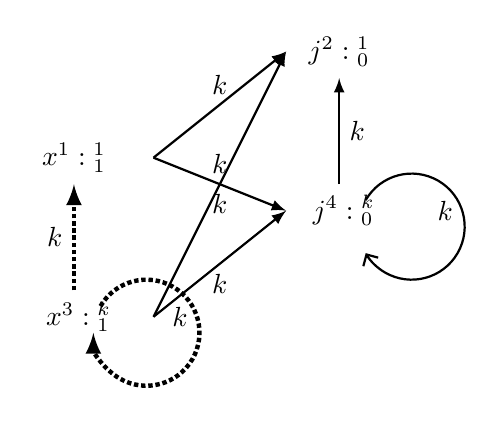
\begin{tikzpicture}[scale=\textwidth/18cm,samples=200]
  \draw[] (0, 7) circle (0pt) node
  {\textbf{$x^1: {}^{1}_{1}$}};
  \draw[] (0, 4) circle (0pt) node
  {{ $x^3: {}^{k}_{1}$}};
  % Counter Variables
  \draw[] (5, 9) circle (0pt) node {{$j^2: {}^{1}_{0}$}};
  \draw[] (5, 6) circle (0pt) node {{ $j^4: {}^{k}_{0}$}};
  %
  % Value Dependency Edges:
  \draw[ ultra thick, -latex, densely dotted,] (0, 4.5)  -- node[left]{\highlight{$k$}} (0, 6.5) ;
  \draw[ ultra thick, -latex, densely dotted,] (0.5, 4.2) arc (150:-180:1);
  \draw[] (2, 4) node []{\highlight{$k$}};
  \draw[ thick, -Straight Barb] (5.5, 6.2) arc (150:-150:1);
  \draw[] (7, 6) node []{\highlight{$k$}};
  \draw[ thick, -latex] (5, 6.5)  -- node[right]{\highlight{$k$}} (5, 8.5) ;
  % Control Dependency
  \draw[ thick,-latex] (1.5, 7)  -- node[above]{\highlight{$k$}} (4, 9) ;
  \draw[ thick,-latex] (1.5, 4)  -- node[above]{\highlight{$k$}} (4, 9) ;
  \draw[ thick,-latex] (1.5, 7)  -- node[below]{\highlight{$k$}} (4, 6) ;
  \draw[ thick,-latex] (1.5, 4)  -- node[below]{\highlight{$k$}} (4, 6) ;
  \end{tikzpicture}
  \caption{}
    \end{centering}
    \end{subfigure}
  }
   \caption{(a) Simple While Loop Example, (b) The Program-Based Dependency Graph generated from $\THESYSTEM$.}
  \label{fig:alg_adaptsearch_simplewhile}
  \end{figure}
  % \begin{figure}
% \centering
% {
% % \footnotesize
% \begin{subfigure}{.25\textwidth}
% \begin{centering}
% $ 
% \begin{array}{l}
%   \kw{whileSim(k)} \triangleq \\
%   \clabel{ \assign{j}{k} }^{0} ; \\
%   \clabel{ \assign{x}{\query(\chi[0])} }^{1} ; \\
%       \ewhile ~ \clabel{j > 0}^{2} ~ \edo ~ \\
%       \Big(
%        \clabel{\assign{x}{\query(\chi[x]) }}^{3}  ; \\
%       \clabel{\assign{j}{j-1}}^{4}       \Big)
%   \end{array}
% $
% \caption{}
% \end{centering}
% \end{subfigure}
% \quad
%   \begin{subfigure}{.6\textwidth}
%   \begin{centering}
%   \begin{tikzpicture}[scale=\textwidth/18cm,samples=200]
% \draw[] (0, 7) circle (0pt) node
% {\textbf{$x^1: {}^{1}_{1}$}};
% \draw[] (0, 4) circle (0pt) node
% {{ $x^3: {}^{k}_{1}$}};
% % Counter Variables
% \draw[] (5, 9) circle (0pt) node {{$j^2: {}^{1}_{0}$}};
% \draw[] (5, 6) circle (0pt) node {{ $j^4: {}^{k}_{0}$}};
% %
% % Value Dependency Edges:
% \draw[ ultra thick, -latex, densely dotted,] (0, 4.5)  -- (0, 6.5) ;
% \draw[ ultra thick, -latex, densely dotted,] (0.5, 4.2) arc (150:-180:1);
% \draw[ thick, -Straight Barb] (5.5, 6.2) arc (150:-150:1);
% \draw[ thick, -latex] (5, 6.5)  -- (5, 8.5) ;
% % Control Dependency
% \draw[ thick,-latex] (1.5, 7)  -- (4, 9) ;
% \draw[ thick,-latex] (1.5, 4)  -- (4, 9) ;
% \draw[ thick,-latex] (1.5, 7)  -- (4, 6) ;
% \draw[ thick,-latex] (1.5, 4)  -- (4, 6) ;
% \end{tikzpicture}
% \caption{}
%   \end{centering}
%   \end{subfigure}
% }
% % \end{wrapfigure}
% % \end{equation*}
% \vspace{-0.4cm}
%  \caption{(a) Simple While Loop Example, (b) The Program-Based Dependency Graph generated from $\THESYSTEM$.}
% \label{fig:alg_adaptsearch_simplewhile}
% \vspace{-0.5cm}
% \end{figure}
% Analysis Results: $ \progA(\kw{whileRec}(k)) = 1 + k$
%
If we traverse on the program-based dependency graph, and decrease the weight of $x^3$ (the weight $k$ is symbolic) by one after every visit,
% We can simply adopt either a deep first strategy to estimate the adaptivity as the length of the longest weight path, as 
% in Algorithm~\ref{alg:overadp_alg}.
we will never terminate because we only know $k \in \mathbb{N}$.

To solve this non-termination challenge, we switch to another walk finding approach: we first find a  longest path in the program-based dependency graph and then approximate the walk with the path.
Through a simple deep first search algorithm, we find the longest weighted path as the dotted arrow in Figure~\ref{fig:alg_adaptsearch_simplewhile},
$x^3: {}^k_1 \to x^1: {}^1_1 $.
Then, by summing up the weights on this path where the vertices has query annotation $1$, deep first search algorithm gives the adaptivity bound $1 + k$.
This is a the tight bound for this program's adaptivity.
% Look at the two-round example in overview, 
% it is easy to find that the longest weighted path is  $x^3 : {}^{k}_{1} \to a^5 : {}^{k}_{0} \to l^6 : {}^{1}_{0}$ with weighted query length $1 + k$.
% If we use this path to approximate a finite walk, and weight of each vertex as
% %  their visiting times, 
% its visiting time,
% then it isn't a qualified walk. 
% In the approximated walk, we have the vertices as $x^3 \to \cdots \to x^3 \to a^5 \to \cdots \to a^5 \to l^6$.

% However, this gives us over-approximation to a large extend in other cases as in \textbf{Approximation Challenge}.
% In Algorithm~\ref{alg:adpt_alg}, 
% we first find all the strong connected components of this graph, 
\textbf{Approximation Challenge:}
% As in Definition~\ref{def:finitewalk}, w
When we adopt a deep first strategy to search for the longest weighted path, and then use the path to approximate the adaptivity. We find that this gives us over-approximation to a large extend.
% Specifically, according to the finite walk definition in Definition~\ref{def:finitewalk},
% the visiting time of every vertex on a walk should be no more than its weight.
% However, by searching for the longest weighted path, 
% % and approximating the finite walk by this weight path, 
% and use it as the approximated finite walk with the longest query length, 
% the visiting times of the vertex on 
% % it 
% this approximated walk could 
% % possibly 
% exceed 
% % its weights. 
% the visiting times it can have.
% Then, this approximated walk isn't a qualified walk by Definition~\ref{def:finitewalk}, 
% and the weighted query length of this path is obviously greater than the maximum query length of the finite walk.
This over-approximation could result in a $\infty$ adaptivity upper bound on the program with actual adaptivity $2$.
Look at the two-round example in overview, 
it is easy to find that the longest weighted path is  $x^3 : {}^{k}_{1} \to a^5 : {}^{k}_{0} \to l^6 : {}^{1}_{0}$ with weighted query length $1 + k$.
If we use this path to approximate a finite walk, and weight of each vertex as
%  their visiting times, 
its visiting time,
then it isn't a qualified walk. 
In the approximated walk, we have the vertices as $x^3 \to \cdots \to x^3 \to a^5 \to \cdots \to a^5 \to l^6$.
Because $l^6$ can only be visited as most once by its weight,
% and this lead to 
resulting in the restriction on the maximum visiting time of $x^3$,
such that $x^3$ is only able to be visited at most once as well.
%
However, $x^3$ is visited $k$ times in this approximated walk.
% Moever, with the longest query length, then 
In order to have $x^3$ be visited $k$ time, we need to go back to 
$x^3$ on this walk from either $a^5$ or $l^6$ for $k$ time.
This is impossible since there is no edge going back to $x^3$ in $\progG(twoRound)$.
Obviously,
% the with the weighted length $1 + k$. It is obviously
its weighted query length, $1 + k$, 
% which is 
over approximates 
% its 
the adaptivity of this example to a large extend, which supposed to be $2$. 
%  for this program, 
% that 


These challenges motivate us to design a walk search algorithm through a combination of 
% DFS and BFS algorithm 
deep first search and breath first search strategy. 
% \wq{
This walk search algorithm consists of two components:
the path searching algorithm, $\pathsearch$ (in Algorithm~\ref{alg:adpt_alg})
which search for a 'suitable' path relying on the strong connected components of the program based dependency graph, 
and $\kw{\pathsearch_{scc}(G)}$ (in Algorithm~\ref{alg:adaptscc}) which approximates the
path.
% path found by Algorithm~\ref{alg:adpt_alg} 
% to a precise walk on the SCC
% and computes the adaptivity.
% These challenges give us the necessary to design a walk search algorithm through a combination of 
% % DFS and BFS algorithm 
% deep first search and breath first search strategy
% % as defined 
% as in Algorithm~\ref{alg:adpt_alg} and Algorithm~\ref{alg:adaptscc}.
%
The $\pathsearch$ as shown in Appendix Algorithm~I, takes our program-based dependency graph as input, and outputs the estimated adaptivity by two steps. 1. Process the input graph to a simplified graph 2. Perform
     the standard breath first search strategy to find the longest weighted path on this simplified graph and return the length as adaptivity.
The step 2 is not interesting, we now discuss step 1. 
The input dependency graph may contain circle due to the while loop, we simplify (shrank) the input graph by replacing every strong connected components(circle) of the graph with, the vertex whose weight is the adaptivity of the SCC 
(a subgraph of the input one) calculated by the $\pathsearch_{\kw{scc}}$. 
The SCC is found by using the Kosaraju's algorithm.
% \wq{cite}. 
The details of this algorithm is explained as follows.
    % This algorithm first finds all the strong connected components (SCC) of $\progG(c)$ using the Kosaraju’s algorithm in line:3. 
    % Every $\kw{SCC_1}, \cdots, \kw{SCC_n}$
    % where $0 \leq n \leq |\vertxs|$ is a sub-graph of $\progG(c)$, where $\kw{SCC_i} = (\vertxs_i, \edges_i, \weights_i, \qflag_i)$.
    % % where $\kw{SCC_i} = (\vertxs_i, \edges_i, \weights_i, \qflag_i)$.
    % Then, 
    % % we compute the adaptivity on every SCC, which is a subgraph of the $\progG(c)$, in line:4-5 by Algorithm~\ref{alg:adaptscc}.
    % it computes the adaptivity on every SCC
    % % , which is a subgraph of the $\progG(c)$, 
    % in line:4-5 by Algorithm~\ref{alg:adaptscc}.
    % % We guarantee the soundness of the adaptivity on SCC by Lemma~\ref{lem:sound_adaptalg_scc} with proof 
    % in Appendix.
    % % ~\ref{apdx:adaptalg_soundness}.
    % The $\progG(c)$ is then shrunk into an acyclic directed graph where 
    % % vertices are all the SCCs and edges are between every SCCs with their adaptivities as weights.
    % $\kw{SCC_1}, \cdots, \kw{SCC_n}$ are vertices with their adaptivities as weights.
    % % , and directed edges are .
    % For every $(v_i, v_j) \in \edges$ such that $v_1 \in \vertxs_i$, $v_j \in \vertxs_j$ and $i \neq j$,
    % there is a edge $(s_i, s_j)$ in this shrank graph. \\ 
    % Then, we use the standard breath first search strategy to find the longest weighted path
    % %  w.r.t. all the SCCs and their adaptivities.
    % on this shrank graph and return the length as adaptivity.
    % \\
%     We guarantee that 
%     % this longest weighted path is a sound computation of the adaptivity on this,
%     the length of this longest weighted path is a sound computation of the adaptivity for program $c$,
%     % as well as 
%     and this longest weighted path a sound computation of the finite walk having the longest query length 
%     % on this graph, in Theorem~\ref{thm:sound_adaptalg}
%     on $c$'s program based dependency graph, in Theorem~\ref{thm:sound_adaptalg}
%     in Appendix.
%     % ~\ref{apdx:adaptalg_soundness}.
% %    
% % \todo{add proof} 
% We also guarantee the conditional completeness of the adaptivity computation for graphs under the case that 
% $c$'s Program-Based Dependency Graph $\progG(c)$ is acyclic directed
% in Theorem~\ref{thm:adaptalg_pcomplete} 
% in Appendix~\ref{apdx:adaptalg_completeness}.
%
\paragraph*{The Adaptivity Computation Algorithm ($\pathsearch$)}
\begin{algorithm}
    \caption{
    {Adaptivity Computation Algorithm ($\pathsearch$)}
    \label{alg:adpt_alg}
    }
    \begin{algorithmic}[1]
    \REQUIRE $G = (\vertxs, \edges, \weights, \qflag)$ \#\{The program based dependency graph\}
    % with a start vertex $s$ and destination vertex $t$ .
    \STATE  {\bf {$\kw{\pathsearch(G)}$}:}  
    \STATE {\bf init} 
    % \\
    % current node: $c$, 
    \\
    $q$: empty queue.
    % \\
    % $\kw{visited}$: List of length $|\vertxs|$, initialize with $\efalse$.
    % \\
    % $\kw{SSCvisited}$: List of length $|\vertxs|$, initialize with $\efalse$.
    % \\ 
    % $\kw{adapt_{scc}(SCC_i) = \pathsearch_{scc}(SCC_i)}$.
    \\
    $\kw{adapt}$ : the adaptivity of this graph initialize with $0$.
    \\
    \STATE Find all Strong Connected Components (SCC) in $G$: $\kw{SCC_1}, \cdots, \kw{SCC_n}, 0 \leq n \leq |\vertxs|$, 
    % where $\kw{SCC_i} = (\vertxs_i, \edges_i, \weights_i, \qflag_i)$.
    % and assign each vertex $x^i$ with an SCC number $\kw{SCC}(x^i)$
    \STATE {\bf for} every SCC: $\kw{SCC_i}$, compute its Adaptivity $\kw{SCC_i}$:
    \STATE \quad $\kw{adapt_{scc}[SCC_i] = \pathsearch_{scc}(SCC_i)}$;
    \STATE {\bf for} every $\kw{SCC_i}$:
    \STATE \qquad $q.append(\kw{SCC_i})$;
    \STATE \qquad $\kw{adapt_{tmp}} = 0$;
    \STATE \qquad {\bf while} $q$ isn't empty:
    \STATE \qquad \qquad $\kw{s} = q.pop()$;  \#\{take the top SCC from head of queue\}
    \STATE \qquad \qquad  $\kw{adapt_{tmp}}_0= \kw{adapt_{tmp}}$; \#\{record the adaptivity of last level\}
    \STATE \qquad \qquad  $\kw{SCC_{max}}$;  \#\{record the SCC with longest walk in this level\}
    % initialize cycle-adapt = 0.
    \STATE \qquad \qquad {\bf for} every 
    % SCC having a directed edge from $s$ of $s$: $\kw{SCC'}$:
    % directed edge goes out of $\kw{s}$ and connects a 
    different SCC, $\kw{s'}$ connected by $\kw{s}$ by a directed edge from $\kw{s}$:
    % \STATE \qquad \qquad   cycle-adapt$ = \max($cycle-adapt, $\kw{dfs_{refine}(G, v, v)})$;
    % \STATE \qquad \qquad \qquad \#\{compute the adaptivity of vertex $v$  on $\kw{SCC}(v)$, and update r[v] with the SCC-adapt\}
    % \STATE \qquad \qquad \qquad $ r[v] = r[s] + \kw{dfs_{refine}(G, v, visited)})$; 
    \STATE \qquad \qquad \qquad {\bf if} $(\kw{adapt_{tmp}} < \kw{adapt_{tmp}}_0 + \kw{adapt_{scc}[s']})$:
    \STATE \qquad \qquad \qquad \qquad $\kw{adapt_{tmp}} = \kw{adapt_{tmp}}_0 + \kw{adapt_{scc}[s']}$; 
    \STATE \qquad \qquad \qquad \qquad $\kw{SCC_{max} = s'} $; \#\{update the SCC with longest walk in this level\} 
    % \STATE \qquad   $r[c] = r[c] + $cycle-adapt;
    % \STATE \qquad for all unvisited vertex $v$ having directed edge from c and $! \kw{cycle}(c)$:
    % \STATE \qquad \qquad $r[v] = r[c] + \flag(v)$; 
    % \STATE \qquad \qquad \qquad  \#\{mark all the nodes with the same $\kw{SCC}$ number as visited\} 
    % \STATE \qquad \qquad \qquad  \#\{append the unvisited vertex to the rear of the queue\}
    % \STATE \qquad \qquad \qquad  \#\{mark all the nodes with the same $\kw{SCC}$ number as visited\} 
    % \STATE \qquad \qquad for $v \in V$,   $\kw{visited}[s] = 1$;
    \STATE \qquad \qquad \qquad $q.append(\kw{SCC_{max}})$;
    \STATE \qquad $\kw{adapt} = \max(\kw{adapt}, \kw{adapt_{tmp}})$;    
    \RETURN $\kw{adapt}$.
    \end{algorithmic}
    \end{algorithm}
    %
%
    % In Algorithm~\ref{alg:adpt_alg}, 
    % it 
    This algorithm first finds all the strong connected components (SCC) of $\progG(c)$ using the Kosaraju’s algorithm in line:3.
    Every $\kw{SCC_1}, \cdots, \kw{SCC_n}$
    where $0 \leq n \leq |\vertxs|$ is a sub-graph of $\progG(c)$, where $\kw{SCC_i} = (\vertxs_i, \edges_i, \weights_i, \qflag_i)$.
    % where $\kw{SCC_i} = (\vertxs_i, \edges_i, \weights_i, \qflag_i)$.
    Then, 
    % we compute the adaptivity on every SCC, which is a subgraph of the $\progG(c)$, in line:4-5 by Algorithm~\ref{alg:adaptscc}.
    it computes the adaptivity on every SCC
    % , which is a subgraph of the $\progG(c)$, 
    in line:4-5 by Algorithm~\ref{alg:adaptscc}.
    We guarantee the soundness of the adaptivity on SCC by Lemma~\ref{lem:sound_adaptalg_scc} with proof in Appendix~\ref{apdx:adaptalg_soundness}.
    The $\progG(c)$ is then shrunk into an acyclic directed graph where 
    % vertices are all the SCCs and edges are between every SCCs with their adaptivities as weights.
    $\kw{SCC_1}, \cdots, \kw{SCC_n}$ are vertices with their adaptivities as weights.
    % , and directed edges are .
    For every $(v_i, v_j) \in \edges$ such that $v_1 \in \vertxs_i$, $v_j \in \vertxs_j$ and $i \neq j$,
    there is a edge $(s_i, s_j)$ in this shrank graph. \\ 
    Then, we use the standard breath first search strategy to find the longest weighted path
    %  w.r.t. all the SCCs and their adaptivities.
    on this shrank graph and return the length as adaptivity.
    \\
    We guarantee that 
    % this longest weighted path is a sound computation of the adaptivity on this,
    the length of this longest weighted path is a sound computation of the adaptivity for program $c$,
    % as well as 
    and this longest weighted path a sound computation of the finite walk having the longest query length 
    % on this graph, in Theorem~\ref{thm:sound_adaptalg}
    on $c$'s program based dependency graph, in Theorem~\ref{thm:sound_adaptalg}
    in Appendix.
    % ~\ref{apdx:adaptalg_soundness}.
%    
% \todo{add proof} 
We also guarantee the conditional completeness of the adaptivity computation for graphs under the case that 
$c$'s Program-Based Dependency Graph $\progG(c)$ is acyclic directed
in Theorem~\ref{thm:adaptalg_pcomplete} 
in Appendix~\ref{apdx:adaptalg_completeness}.
    % for every vertex which isn't on any SCC, it is easy to know that it will be visited 
    % at most once given no edges going back to this vertex. We can know the adaptivity on the SCC 
     %
    % \begin{algorithm}
    % \caption{
    % {Longest Adaptivity Search Algorithm ($\pathsearch$)}
    % \label{alg:adpt_alg}
    % }
    % \begin{algorithmic}
    % \REQUIRE Weighted Directed Graph $G = (\vertxs, \edges, \weights, \flag)$ with a start vertex $s$ and destination vertex $t$ .
    % \STATE  {\bf {bfs $(G)$}:}  
    % \STATE {\bf init} 
    % \\
    % current node: $c$, 
    % \\
    % queue: $q$ : List, add into $a$ an arbitrary v from $\vertxs$. 
    % \\
    % visited: List of length $|\vertxs|$, initialize with $\efalse$.
    % \\
    % results: $r$ : List of length $|\vertxs|$, initialize with -1.
    % \\
    % curr$\kw{flowcapacity}$: INT, initialize MAXINT.
    % \\
    % querynum: INT, initialize 0. \#\{To count the query numbers when we are walking inside a cycle\}
    % \\
    % \STATE \qquad {\bf while} $q$ isn't empty:
    % \STATE \qquad \qquad take the vertex from head $c= q.pop()$
    % \STATE \qquad \qquad mark $c$ as visited, visited $[c] = 1$.
    % \STATE \qquad \qquad {\bf if} $\kw{cycle}(c)$  \#\{we are inside a cycle\}
    % \STATE \qquad \qquad \qquad curr$\kw{flowcapacity}$ = min($\weights$(c), curr$\kw{flowcapacity}$).
    % \STATE \qquad \qquad \qquad querynum += $\flag(c)$.
    % \STATE \qquad \qquad  \qquad for all unvisited vertex $v$ having directed edge from c:
    % \STATE \qquad \qquad \qquad \qquad r[v] = r[c]; q.add(v)
    % \STATE \qquad \qquad \qquad  {\bf if}  $v$ is visited, then the circle finished
    % \STATE \qquad \qquad \qquad \qquad update the result $r[v] =  \max(r[v], r[c] + $curr$\kw{flowcapacity}$*querynum)
    % \STATE \qquad \qquad \qquad \qquad curr$\kw{flowcapacity}$ = MAXINT
    % \STATE \qquad \qquad \qquad \qquad querynum = 0.  
    % \STATE \qquad \qquad {\bf else} 
    % \STATE \qquad \qquad \qquad for all unvisited vertex $v$ having directed edge from c:
    % \STATE \qquad \qquad \qquad  \qquad $r[v] = \max(r[v], r[c] + \flag(c))$; q.add(v)
    % \RETURN max($r$)
    % \end{algorithmic}
    % \end{algorithm}
    %
%
    % \begin{algorithm}
    %     \caption{
    %     {Over-Approximated Adaptivity on SCC}
    %     \label{alg:overadp_alg}
    %     }
    %     \begin{algorithmic}
    %     \REQUIRE Weighted Directed Graph $G = (\vertxs, \edges, \weights, \qflag)$ with a start vertex $s$ and destination vertex $t$ .
    %     \STATE  {\bf {$\kw{dfs_{naive}(G, c,visited)}$}:}  
    %     % \STATE {\bf init} 
    %     % \\
    %     % current node: $c$, 
    %     % \\
    %     % visited: List of length $|\vertxs|$, initialize with $\efalse$.
    %     % \\
    %     % \STATE {\bf if} $c = s$:
    %     % \RETURN \qquad  $\weights(s)*\flag(s) $.
    %     \STATE $r[c] = \weights(c)*\qflag(c) $
    %     \STATE {\bf for}  all vertex $v$ having directed edge from $c$:
    %     \STATE \qquad {\bf if}  $v$ is unvisited:
    %     \STATE \qquad \qquad  \#\{mark $v$ as visited\} $\kw{visited}[v] = 1$;
    %     \STATE \qquad \qquad $r[c] += \kw{dfs_{naive}(G, v, visited)}$;
    %     % \STATE \qquad {\bf else}: \#\{There is a cycle finished\}
    %     % \RETURN \qquad \qquad $\weights(v)*\flag(v) $.
    %     \RETURN $r[c]$
    %     \end{algorithmic}
    %     \end{algorithm}%
        %
  \paragraph*{Adaptivity Computation Algorithm on SCC Graph ($\kw{\pathsearch_{scc}(G)}$)}
    \begin{algorithm}
            \caption{
            {Adaptivity Computation Algorithm on SCC Graph }
            \label{alg:adaptscc}
            }
            \begin{algorithmic}[1]
              \REQUIRE $G = (\vertxs, \edges, \weights, \qflag)$ \#\{An Strong Connected program based dependency Graph\}
            \STATE  {\bf {$\kw{\pathsearch_{scc}(G)}$}:}  
            \STATE {\bf init} 
            \\
            $\kw{r_{scc}}$: $EXPR(\constdom)$, initialized $0$, the Adaptivity of this SCC
            \STATE \qquad {\bf init} 
            % \STATE \qquad current node: $c$, 
            % \\
            % visited: List of length $|\vertxs|$, initialize with $\efalse$.
            % \\ \qquad  $\kw{r_{scc}}$ : initialize $0$, the adaptivity of this graph
            \\ \qquad  $\kw{visited}$ : $\{0, 1\}$ List, 
            \\ \qquad  \#\{length $|\vertxs|$, initialize with $0$ for every vertex, recording whether a vertex is visted.\}
            \\ \qquad  $\kw{r}$ : $EXPR(\constdom)$ List, 
            \\ \qquad  \#\{length $|\vertxs|$, initialize with $\qflag(v)$ for every vertex, recording the adaptivity reaching each vertex.\}
            \\ \qquad  $\kw{flowcapacity}$: $EXPR(\constdom)$ List, 
            % INT List of length $|\vertxs|$, initialize MAXINT. 
            \\ \qquad  \#\{length $|\vertxs|$, initialize with $\infty$ for every vertex,
            % \#\{For every vertex, 
            recording the minimum weight when the walk reaching 
            that vertex, inside a cycle\}
            \\ \qquad  $\kw{querynum}$: INT List,
            %  of length $|\vertxs|$, initialize with $\qflag(v)$ for every vertex. 
            \\ \qquad  \#\{length $|\vertxs|$, initialize with $\qflag(v)$ for every vertex, 
            % \#\{For every vertex, 
            recording the query numbers when the path reaching 
            that vertex, inside a cycle\}
            \STATE {\bf if} $|\vertxs| = 1$ and $|\edges| = 0$:
            \STATE \qquad {\bf return}  $\qflag(v)$
            \STATE  {\bf def} {$\kw{dfs(G, c,visited)}$}:
            % \STATE \qquad update the length of the longest path reaching this vertex
            % $r[s] =  r[s] + $$\kw{flowcapacity}$[s] * querynum[s].
            % \RETURN  \qquad $r[s]$.      
            \STATE \qquad {\bf for} every vertex $v$ 
            % having directed edge from $c$:
            connected by a directed edge from $c$:
            \STATE \qquad \qquad {\bf if} $\kw{visited}[v] = \efalse$:
            \STATE \qquad \qquad \qquad $\kw{flowcapacity[v] = \min(\weights(v), {flowcapacity}[c])}$;
            \STATE \qquad \qquad \qquad $\kw{querynum[v] = querynum[c] + \qflag(v)}$;
            % \STATE \qquad \qquad \qquad \#\{do not update the length of the longest walk reaching $v$ until the cycle is finished\}
            % \STATE \qquad \qquad \qquad $\kw{r[v] =  r[c] + flowcapacity[v] \times querynum[v]} $; \#\{do not update the length of the longest walk reaching $v$ until the cycle is finished\}
            \STATE \qquad \qquad \qquad $\kw{r[v] =  \max(r[v], flowcapacity[v] \times querynum[v]}) $; 
            % \#\{do not update the length of the longest walk reaching $v$ until the cycle is finished\}
            \STATE \qquad \qquad \qquad  $\kw{visited}[v] = 1$; %\#\{mark $v$ as visited\}
            \STATE \qquad \qquad \qquad $\kw{dfs(G, v, visited)}$;
            \STATE \qquad \qquad {\bf else}: \#\{There is a cycle finished\}
            % \STATE \qquad \qquad \qquad \#\{update the length of the longest path reaching this vertex\}
            \STATE \qquad \qquad \qquad 
            $\kw{r[v] =  \max(r[v], r[c] +  \min(\weights(v), {flowcapacity}[c]) * (querynum[c] + \qflag(v)))}$; \#\{update the length of the longest walk reaching this vertex on this cycle\}
            %  $\kw{r[v] =  \max(r[v], r[c] + flowcapacity[v] * querynum[v])}$; \#\{update the length of the longest walk reaching this vertex on this cycle\}
            %  \STATE \qquad \qquad \qquad \#\{Recover the $\kw{flowcapacity}$ and querynumber to previous state, for different loops\}
            % \STATE \qquad \qquad \qquad $\kw{flowcapacity[v] = flowcapacity[c]}$; \#\{Recover the $\kw{flowcapacity}$\}
            % \STATE \qquad \qquad \qquad $\kw{querynum[v] = querynum[c]}$;\#\{Recover the $\kw{querynum}$\}
            \STATE \qquad {\bf return}  $\kw{r[c]}$
            \STATE  {\bf for} every vertex $v$ in $\vertxs$:
            \STATE  \qquad initialize the $\kw{visited, r, flowcapacity, querynum}$;
            \STATE  \qquad $\kw{r_{scc} = \max(r_{scc}, dfs(G, v, \kw{visited} ))}$ ; 
            \RETURN  $\kw{r_{scc}}$
            \end{algorithmic}
            \end{algorithm}
            % \\
% Following is the challenge of computing the adaptivity on a program based dependency graph.
% In order to search for the finite walk having the longest query length, which isn't a simple longest weighted path.
% \\
% the visiting times of every vertex on this walk should be no more than its weight, which is a symbolic expression.
% So we cannot simply search for the longest weight path where the visiting times of the vertex on it could possibly exceed its weights.
% We can neither simply traverse on this graph by decreasing the weight of every node by 1 after every visiting,
% because the weight is symbolic and simply traversing leads to non-termination.
% \\
% In Algorithm~\ref{alg:adaptscc}, 
This algorithm takes a subgraph of the program-based dependency graph as input, to be precise, the input graph is SCC, and the output is the adaptivity of this SCC. 
For an SCC containing only one vertex without any edge, it returns the query annotation of this vertex as adaptivity.
For SCC containing at least one edge, 
There are three steps in this algorithm: 1. find out all the paths in the input SCC 2. Calculate the adaptivity of every path using our designed adaptivity counting method. 3. Return the maximal adaptivity among all the paths. The step 3 is trivial. Because our input graph is SCC, when we start traversing from a vertex, we will finally go back to this vertex. The paths we find in step 1 are all those with the same starting and ending vertex. The most interesting part is step 2. 
We discuss as follows.

This algorithm first check if an SCC contains only one vertex without any edge, as in line:4-5 in Algorithm~\ref{alg:adaptscc}.
% then 
% \\
% If yes, then it's easy to know that it will be visited 
% at most once since there isn't edge going back to this vertex. 
% So we can know that the adaptivity on this SCC is at most one if it is a query vertex,
% and zero otherwise.
% \\
% If not, then 
Again, for 
the SCC containing only one vertex without any edge, as in line:4-5 in Algorithm~\ref{alg:adaptscc}.
% then 
% If yes, then i
% it's easy to know that it will be visited 
% at most once since there isn't edge going back to this vertex. 
% So we can know 
The adaptivity on this SCC is at most one if it is a query vertex,
and zero otherwise.
$\kw{\pathsearch_{scc}(G)}$ return query annotation directly as in line:4-5.
% So $\kw{\pathsearch_{scc}(G)}$ return query annotation directly as in line:4-5.
\\
% For the SCC contains at least one edge, we are searching for the finite walk having the longest query length through a deep first search strategy.
For the SCC containing at least one edge, 
we compute the adaptivity for each path 
on the fly of searching for the paths 
in the
% design a 
recursion algorithm $\kw{dfs}$ designed based on 
a deep first search strategy 
% of this algorithm is described as follows,
from line: 6-16 in $\kw{\pathsearch_{scc}(G)}$ in Algorithm~\ref{alg:adaptscc}.
\\
% The difficulty is, the visiting times of every vertex on this walk should be no more than its weight, which is a symbolic expression.
% As the two challenges discussed above, we want to guarantee the visiting time of each vertex smaller than 
% its weight, in the meantime the algorithm termination. 
% Additionally, we are computing the query length rather than sum of the weights.
% We design a deep first search strategy
% % of this algorithm is described as follows,
% from line: 6-16 in Algorithm~\ref{alg:adaptscc}, 
% searching for the finite walk having the longest query length
% %  through a deep first search strategy
% with a capacity limitation and use special parameter to compute the adaptivity.
%
As the \textbf{Approximation Challenge} discussed above, 
we want to guarantee the visiting time of each vertex smaller than 
its weight and compute the adaptivity accurately, in the meantime guarantee the algorithm termination. 
It uses a capacity limitation and  special parameters to achieve it,
specifically as follows.
Additionally, we are computing the query length rather than sum of the weights.
We design a deep first search strategy
% of this algorithm is described as follows,
from line: 6-16 in Algorithm~\ref{alg:adaptscc}, 
% searching for the finite walk having the longest query length
%  through a deep first search strategy
with a capacity limitation and use special parameter to compute the adaptivity.
% for every path.
%
% for every path.
% So we cannot simply search for the longest weight path where the visiting times of the vertex on it could possibly exceed its weights.
% We can neither simply traverse on this graph by decreasing the weight of every node by 1 after every visiting,
% because the weight is symbolic and simply traversing leads to non-termination.
% \\
\\
In order to
guarantee the termination, 
% this algorithm 
$\kw{\pathsearch_{scc}(G)}$
terminates the recursion if monitored a cycle, as in line:8 and line:14, through a boolean list $\kw{visited}$.
This guaranteed the termination and solved the \textbf{Challenge II.} discussed above.
% \todo{solve the challenge 2} 
% search for finite walk  
% So we use the dfs to search for the 
\\
% In order to
% solve the \textbf{Challenge I},
% specifically guarantee the visiting times of each vertex by its weight, 
% we use a special parameter $\kw{flowcapacity}$  to track the minimum weight during the 
% % dfs process, 
% deep first searching along the walk, 
% also a parameter $\kw{querynum}$
% % to compute the query length of this walk
% to track the total number of vertices which are query vertices along the walk in order to compute the query length of this walk.
In order to
solve the \textbf{Approximation Challenge},
specifically guarantee the visiting times of each vertex by its weight
and compute the adaptivity accurately, 
we use a special parameter $\kw{flowcapacity}$  to track the minimum weight
along the path during the 
% dfs process, 
% deep first 
searching procedure, 
and a parameter $\kw{querynum}$
% to compute the query length of this walk
to track the total number of vertices with query annotation $1$
% which are query vertices 
along the path 
in order to compute the query length.
% 
% \todo{solve the challenge 1, specifically in the dfs strategy
% of this algorithm is described as follows,
% from line: 6-16 in Algorithm~\ref{alg:adaptscc}. } 
% \\
% Then, to compute the query length of this walk, 
% we use another parameter $\kw{querynum}$
% to track the total number of vertices which are query vertices along the walk.

The detail steps of this dfs strategy
% of this algorithm is described as follows,
from line: 3-16 in Algorithm~\ref{alg:adaptscc},
particularly from line: 7-15 on how to 
use these two special parameters to resolve \textbf{Approximation Challenge}
 is described as follows.
 %
 $\kw{flowcapacity}$ is a list of symbolic expressions for every vertex, recording the minimum weight when the path reaches that vertex, which is initialized by $\infty$.
% , inside a cycle\}

$\kw{querynum}$ is a list of integer with length $|\vertxs|$, which is initialized with $\qflag(v)$ for every vertex. 
For every vertex, 
% recording the query numbers when the path reaching.
% in order to 
it records the total query numbers when the path reaching this vertex.

We maintain the minimum weight for the 
$\kw{flowcapacity}$, 
number of query vertices 
$\kw{querynum}$ 
and update the adaptivity for this path $\kw{r}$
alone the path and update the adaptivity reaching 
this vertex, 
when traversing on this graph, as in Algorithm~\ref{alg:adaptscc} from line: 8-13.
% and then recursively dfs on all vertices heading out from this vertex.
% \\
At line: 15 where this vertex is visited, i.e., this path 
going back to its starting node,
we only update the adaptivity $\kw{r}$ reaching this vertex.
% and neither recursion nor update the $\kw{flowcapacity}$  and 
% $\kw{querynum}$.
\\
% Again, Non-recursion in the second branch
% % in order to 
% guarantees the termination and resolves \textbf{Non-Termination Challenge}.
% \\
The updating operations
during the traversing 
(in line: 11) and 
at the end of the traverse (in line: 15),
% in these two branches, 
specifically the $\kw{flowcapacity[v] \times querynum[v]}$ 
% in line: 11 and line: 15 
computes the query length for this path. 
it guarantees 
the visiting times of each vertex on the path reaching a vertex $v$ is no more than 
the maximum visiting it can be on a qualified walk, through $\kw{flowcapacity[v]}$,
and in the same time  compute the query length instead of weighted length accurately through 
$\kw{ querynum[v]}$.
%  its minimum visiting time, 
In this way, we resolve the \textbf{Approximation Challenge} and in the same time without losing the soundness,
% searching for the finite walk having the longest query length through a deep first search strategy
% with a capacity limitation and use special parameter to compute the adaptivity
% for every path.
\\
We first initialize some parameters:
\\
$\kw{visited}$ is initialized as a list of $0$ for every vertex on this SCC, in order to guarantee the termination;
\\ 
$\kw{r}$ is initialized  as a list of integer with length $|\vertxs|$, initialize with $\qflag(v)$ for every vertex. The adaptivity reaching each vertex.
\\ 
$\kw{flowcapacity}$ a list of symbolic expressions for every vertex, recording the minimum weight when the walk reaching that vertex, which  is initialized by $\infty$.
% , inside a cycle\}
\\ 
$\kw{querynum}$ is a list of integer with length $|\vertxs|$, which is initialized with $\qflag(v)$ for every vertex. 
For every vertex, 
% recording the query numbers when the path reaching.
in order to record the total query numbers when the walk reaches a vertex.
\\
Then from line: 5-11, we record the minimum weight and number of query vertices alone the path and update the adaptivity reaching 
this vertex, and then recursively dfs on all vertices heading out from this vertex.
\\
At line: 12 where this vertex is visited, 
we only update the adaptivity reaching this vertex and neither recursion nor update the $\kw{flowcapacity}$  and 
$\kw{querynum}$.
% \\
% Again, Non-recursion in the second branch
% % in order to 
% guarantees the termination and resolves \textbf{Challenge I}.
\\
The updating operation in these two branches, 
specifically $\kw{flowcapacity[v] \times querynum[v]}$ in line: 11 and line: 15 
guarantees 
1.the visiting times of each vertex on the walk reaching $v$ is no more than 
the maximum visiting it can be on this walk, through $\kw{flowcapacity[v]}$. 
%  its minimum visiting time, 
In this way, we resolve the \textbf{Approximation Challenge}  and in the same time without losing the soundness 
% this 
% 2. then 
by using $\kw{flowcapacity[v] \times querynum[v]}$ to compute the query length. 
% without lose the adaptivity.
%
\\
Notice here, another special operation we have in the second branch is Non-updating of
% Non-updating the 
$\kw{querynum}$ and $\kw{flowcapacity}$.
This guarantees both the accuracy and the soundness, formally in Lemma~\ref{thm:sound_adaptalg} in Appendix~\ref{apdx:adaptalg_soundness}.

Now, we show an example illustrating how our two updating operations for adaptivity 
for each path can guarantee both the accuracy and the soundness. 
Look at a Nested While Loop example program in Figure~\ref{fig:alg_adaptsearch_nestedwhile}.
% Notice here, another special operation we have in the second branch is Non-updating of
% % Non-updating the 
% $\kw{querynum}$ and $\kw{flowcapacity}$.
% This guarantees both the accuracy and the soundness.
% Specifically,
% % because a second visiting of the same vertex 
% if this vertex is visited, it indicates that a cycle is monitored and  
% % indicates there is a cycle goes back to this vertex, 
% the traversing on this cycle is finished by going back to this vertex.
% %
% % then, when 
% When we continuously search for walks heading out of this vertex, 
% the minimum weight on this cycle does not affect the walks going out of this vertex that not pass this cycle.
% However, if we keep recording the minimum weight, then we
% %  are restricting 
% restrict the visiting times of vertices on a walk by
%  using the minimum weight of vertices not on this walk.
% %  , it is unsound anymore.
% Then, it is obviously that this leads to unsoundness.
% \todo{example} 
% To under stand how the two operations 
We first search for a path: $y^6 \to y^6$, and compute the adaptivity for this path as 
$k$.
Notice here, another special operation we have in the second branch is Non-updating of
% Non-updating the 
$\kw{querynum}$ and $\kw{flowcapacity}$.
This guarantees both the accuracy and the soundness.
Specifically,
% because a second visiting of the same vertex 
if this vertex is visited, it indicates that a cycle is monitored and  
% indicates there is a cycle goes back to this vertex, 
the traversing on this cycle is finished by going back to this vertex.
%
% then, when 
When we continuously search for walks heading out of this vertex, 
the minimum weight on this cycle does not affect the walks going out of this vertex that not pass this cycle.
However, if we keep recording the minimum weight, then we
%  are restricting 
restrict the visiting times of vertices on a walk by
using the minimum weight of vertices not on this walk.
%  , it is unsound anymore.
Then, it is obviously that this leads to unsoundness.
If we update the $\kw{flowcapacity}[y^6]$ as $k$ after visiting $y^6$ the second time 
on this walk,
% the walk $y^6 \to y^6$,
and continuously visit $x^9$,
then the $\kw{flowcapacity[k]}$ is 
updated as $\min(k, k^2)$.
So
%  which 
% restricting 
the visiting times of $x^9$ is restricted by $k$ on the walk $y^6 \to y^6 \to x^9$.
This restriction excludes the finite walk $y^6 \to y^6 \to x^9 \to x^9$ where $y^6$ and $x^9$ visited by $k^2$ times
in the computation. 
However, the finite walk $y^6 \to y^6 \to x^9 \to x^9$ where $y^6$ is visited $k$ times and $x^9$ $k^2$ times is 
a qualified walk, and exactly the longest walk we aim to find. So, by Non-updating the $\kw{flowcapacity}$ after 
visiting $y$ again, we guarantee that the visiting times og vertices on every searched walk will not be restricted by weights not on this walk,
i.e., the soundness.
\\
In the last line of this dfs algorithm, line: 16, it returns the adaptivity heading out from its input vertex.
\\
By applying this deep first search strategy on every vertex on this SCC, 
we compute the adaptivity of this SCC by taking the maximum 
% adaptivity reaching every vertex on this SCC.
value over every vertex.
%
The soundness is formally guaranteed in Lemma~\ref{lem:sound_adaptalg_scc} in Appendix~\ref{apdx:adaptalg_soundness}.

% Look at a Nested While Loop example program in Figure~\ref{fig:alg_adaptsearch_nestedwhile}.

% Specifically,
% % because a second visiting of the same vertex 
% if this vertex is visited, it indicates that a cycle is monitored and  
% % indicates there is a cycle goes back to this vertex, 
% the traversing on this cycle is finished by going back to this vertex.
% %
% % then, when 
% When we continuously search for walks heading out of this vertex, 
% the minimum weight on this cycle does not affect the walks going out of this vertex that not pass this cycle.
% However, if we keep recording the minimum weight, then we
% %  are restricting 
% restrict the visiting times of vertices on a walk by
%  using the minimum weight of vertices not on this walk.
% %  , it is unsound anymore.
% Then, it is obviously that this leads to unsoundness.
 %
  %
  \begin{figure}
    \centering
    {\footnotesize
    \begin{subfigure}{.4\textwidth}
    \begin{centering}
    % 
    $ 
    \begin{array}{l}
      \kw{nestedWhileMultiVarRecAcross}(k) \triangleq \\
      \clabel{\assign{i}{k} }^{0} ; \\
      \clabel{ \assign{x}{\query(\chi[0])}}^{1} ; \\
      \clabel{ \assign{y}{\query(\chi[1])}}^{2} ; \\
          \ewhile ~ \clabel{i > 0}^{3} ~ \edo ~ \\
          \Big(
           \clabel{\assign{i}{i-1}}^{4} ;\\
           \clabel{\assign{j}{k}}^{5} ;\\
           \clabel{\assign{y}{\query(\chi(\ln(x) + y))} }^{6}  ; \\
           \ewhile ~ \clabel{j > 0}^{7} ~ \edo ~ \\
           \Big(
            \clabel{\assign{j}{j-1}}^{8};\\
            \clabel{\assign{x}{\query(\chi(\ln(y))+\chi[x])} }^{9}
            \Big) \Big)
      \end{array}
    %       
    $
    \caption{}
    \end{centering}
    \end{subfigure}
    \quad
    \begin{subfigure}{.52\textwidth}
      \begin{centering}
      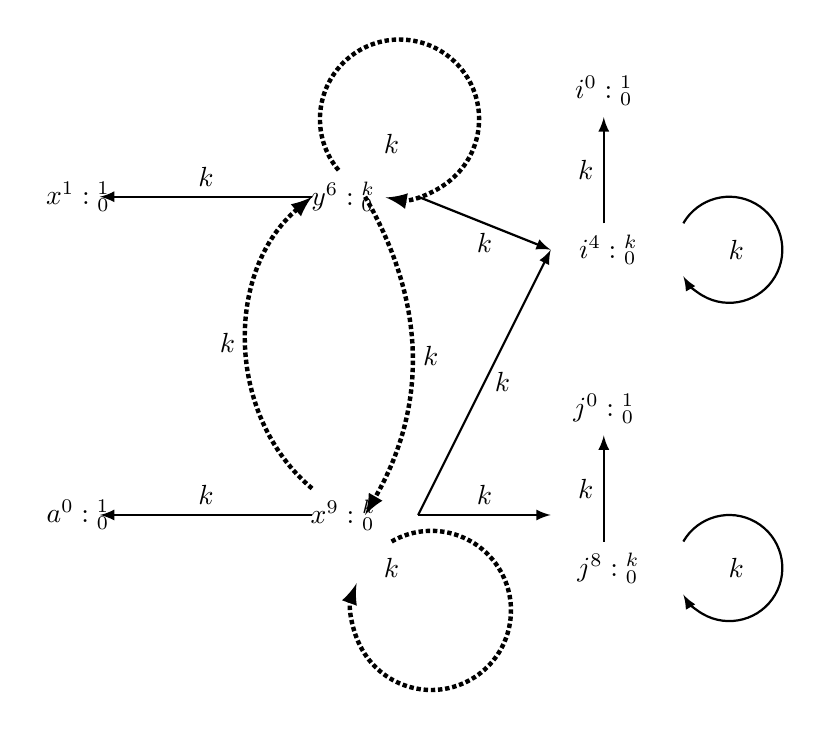
\begin{tikzpicture}[scale=\textwidth/18cm,samples=200]
      % Variables Initialization
      \draw[] (-5, 1) circle (0pt) node{{ $a^0: {}^1_{0}$}};
      \draw[] (-5, 7) circle (0pt) node{{ $x^1: {}^{1}_{0}$}};
      % Variables Inside the Loop
      \draw[] (0, 7) circle (0pt) node{{ $y^6: {}^{k}_{0}$}};
      \draw[] (0, 1) circle (0pt) node{{ $x^9: {}^{k}_{0}$}};
      % Counter Variables
      \draw[] (5, 9) circle (0pt) node {{$i^0: {}^{1}_{0}$}};
      \draw[] (5, 6) circle (0pt) node {{ $i^4: {}^{k}_{0}$}};
      \draw[] (5, 3) circle (0pt) node {{$j^0: {}^{1}_{0}$}};
      \draw[] (5, 0) circle (0pt) node {{ $j^8: {}^{k}_{0}$}};
      % Value Dependency Edges:
      \draw[ ultra thick, -latex, densely dotted,] (0, 7.5) arc (220:-100:1.5);
      \draw[] (1, 8) node [] {\highlight{$k$}};
      \draw[ thick, -latex] (5, 6.5)  -- node[left]{\highlight{{$k$}}}(5, 8.5) ;
      \draw[ thick, -latex] (5, 0.5)  -- node[left]{\highlight{{$k$}}}(5, 2.5) ;
      \draw[ ultra thick, -latex, densely dotted,] (1., 0.5) arc (120:-200:1.5);
      \draw[] (1, 0) node [] {\highlight{$k$}};
      % Value Dependency Edges on Initial Values:
      \draw[ thick, -latex,] (-0.5, 1)  -- node[above]{\highlight{{$k$}}}(-4.5, 1) ;
      \draw[ thick, -latex,] (-0.5, 7)  -- node[above]{\highlight{{$k$}}}(-4.5, 7) ;
      %
      \draw[ ultra thick, -latex, densely dotted,] (-0.5, 1.5)  to  [out=-220,in=220]  
      node[left]{\highlight{{$k$}}}(-0.5, 7);
      \draw[ ultra thick, -latex, densely dotted,]  (0.5, 7) to  [out=-60,in=60] 
      node[right]{\highlight{{$k$}}}(0.5, 1) ;
      % Control Dependency
      \draw[ thick, -latex, ] (6.5, 6.5) arc (150:-150:1);
      \draw[] (7.5, 6) node [] {\highlight{$k$}};
      \draw[ thick, -latex, ] (6.5, 0.5) arc (150:-150:1);
      \draw[] (7.5, 0) node [] {\highlight{$k$}};
      \draw[ thick,-latex] (1.5, 7)  -- node[below]{\highlight{{$k$}}}(4, 6) ;
      \draw[ thick,-latex] (1.5, 1)  -- node[right]{\highlight{{$k$}}}(4, 6) ;
      \draw[ thick,-latex] (1.5, 1)  -- node[above]{\highlight{{$k$}}}(4, 1) ;
   \end{tikzpicture}
   \caption{}
      \end{centering}
      \end{subfigure}
    }
     \caption{(a) Nested While Loop Example, (b) Execution-Based Dependency Graph, (c) The Static Program-Based Dependency graph.}
    \label{fig:alg_adaptsearch_nestedwhile}
    \vspace{-0.5cm}
    \end{figure}
    %
%     When we searched for a walk: $y^6 \to y^6$,
%   if we update the $\kw{flowcapacity}[y^6]$ as $k$ after visiting $y^6$ the second time 
%   on this walk,
%   % the walk $y^6 \to y^6$,
%   and continuously visit $x^9$,
%   then the $\kw{flowcapacity[k]}$ is 
%   updated as $\min(k, k^2)$.
%   So
%   %  which 
%   % restricting 
%   the visiting times of $x^9$ is restricted by $k$ on the walk $y^6 \to y^6 \to x^9$.
%   This restriction excludes the finite walk $y^6 \to y^6 \to x^9 \to x^9$ where $y^6$ and $x^9$ visited by $k^2$ times
%   in the computation. 
%   However, the finite walk $y^6 \to y^6 \to x^9 \to x^9$ where $y^6$ is visited $k$ times and $x^9$ $k^2$ times is 
%   a qualified walk, and exactly the longest walk we aim to find. So, by Non-updating the $\kw{flowcapacity}$ after 
%   visiting $y$ again, we guarantee that the visiting times og vertices on every searched walk will not be restricted by weights not on this walk,
%   i.e., the soundness.
%  \\
% In the last line of this dfs algorithm, line: 16, it returns the adaptivity heading out from its input vertex.
% \\
% By applying this deep first search strategy on every vertex on this SCC, 
% we compute the adaptivity of this SCC by taking the maximum 
% % adaptivity reaching every vertex on this SCC.
% value over every vertex.
% %
% The soundness is formally guaranteed in Lemma~\ref{lem:sound_adaptalg_scc} in Appendix~\ref{apdx:adaptalg_soundness}.
            % \begin{algorithm}
        % \caption{
        % {Refined Adaptivity on $\kw{SCC}$}
        % \label{alg:dfscycle_alg}
        % }
        % \begin{algorithmic}
        % \REQUIRE Weighted Directed Graph $G = (\vertxs, \edges, \weights, \qflag)$ with a start vertex $s$ and destination vertex $t$ .
        % \STATE  {\bf {$\kw{dfs_{refine}(G, c, visited)}$}:}  
        % \STATE {\bf init} 
        % \\
        % current node: $c$, 
        % % \\
        % % visited: List of length $|\vertxs|$, initialize with $\efalse$.
        % \\
        % results: $r$ : INT List of length $|\vertxs|$, initialize with $\qflag(v)$ for every vertex.
        % \\
        % $\kw{flowcapacity}$: INT List of length $|\vertxs|$, initialize MAXINT. 
        % \#\{For every vertex, recording the minimum weight when the walk reaching 
        % that vertex, inside a cycle\}
        % \\
        % querynum: INT List of length $|\vertxs|$, initialize with $\qflag(v)$ for every vertex. 
        % \#\{For every vertex, recording the query numbers when the walk reaching 
        % that vertex, inside a cycle\}
        % \\
        % % \STATE {\bf if} $c = s$:
        % % \STATE \qquad update the length of the longest path reaching this vertex
        % % $r[s] =  r[s] + $$\kw{flowcapacity}$[s] * querynum[s].
        % % \RETURN  \qquad $r[s]$.      
        % \STATE {\bf for}  all vertex $v$ having directed edge from $c$:
        % \STATE \qquad \qquad $\kw{flowcapacity}$[v] = min($\weights(v)$, $\kw{flowcapacity}$[c]);
        % \STATE \qquad \qquad querynum[v] = querynum[c] + $\qflag(v)$;
        % \STATE \qquad \qquad \#\{do not update the length of the longest walk reaching $v$ until the cycle is finished\}
        % \STATE \qquad \qquad $r[v] =  r[c] $;
        % \STATE \qquad {\bf if}  $v$ is unvisited:
        % \STATE \qquad \qquad \#\{mark $v$ as visited\} $\kw{visited}[v] = 1$;
        % \STATE \qquad \qquad $\kw{dfs_{refine}(G, v, visited)}$;
        % \STATE \qquad {\bf else}: \#\{There is a cycle finished\}
        % \STATE \qquad \qquad \#\{update the length of the longest path reaching this vertex\}
        % \STATE \qquad \qquad 
        %  $r[v] =  \max(r[v], r[c] + $$\kw{flowcapacity}$[v] * querynum[v]);
        %  \STATE \qquad \qquad \#\{Recover the $\kw{flowcapacity}$ and querynumber to previous state, for different loops\}
        %  \STATE \qquad \qquad $\kw{flowcapacity}$[v] = $\kw{flowcapacity}$[c];
        %  \STATE \qquad \qquad querynum[v] = querynum[c];
        % \RETURN  $r[c]$
        % \end{algorithmic}
        % \end{algorithm}
        % %
        \begin{algorithm}
          \caption{
          {Over-Approximated Adaptivity on SCC}
          \label{alg:overadp_alg}
          }
          \begin{algorithmic}[1]
          \REQUIRE $G = (\vertxs, \edges, \weights, \qflag)$ \#\{An Strong Connected Symbolic Weighted Directed Graph\}
          % with a start vertex $s$ and destination vertex $t$ .
          \STATE {\bf {$\kw{\pathsearch_{scc-naive}(G)}$}:}  
          \STATE {\bf init} 
          \\
          $\kw{r_{scc}}$: the Adaptivity of this SCC
          % \STATE  {\bf def} {$\kw{dfs_{naive}(G, c,visited)}$}: 
          % % \STATE {\bf init} 
          % % \\
          % % current node: $c$, 
          % % \\
          % % visited: List of length $|\vertxs|$, initialize with $\efalse$.
          % % \\
          % % \STATE {\bf if} $c = s$:
          % % \RETURN \qquad  $\weights(s)*\flag(s) $.
          % \STATE \qquad $r[c] = \weights(c)*\qflag(c) $
          % \STATE \qquad {\bf for}  all vertex $v$ having directed edge from $c$:
          % \STATE \qquad \qquad {\bf if}  $v$ is unvisited:
          % \STATE \qquad \qquad \qquad  \#\{mark $v$ as visited\} $\kw{visited}[v] = 1$;
          % \STATE \qquad \qquad \qquad $r[c] += \kw{dfs_{naive}(G, v, visited)}$;
          % \STATE \qquad {\bf else}: \#\{There is a cycle finished\}
          % \RETURN \qquad \qquad $\weights(v)*\flag(v) $.
          \STATE  {\bf for} every vertex $v$ in $\vertxs$:
          % \STATE  \qquad initialize \kw{visited} with $\efalse$.
          \STATE  \qquad $r_{scc} += \weights(v)*\qflag(v)$  
          \RETURN $r[c]$
          \end{algorithmic}
          \end{algorithm}
          %
\begin{thm}[Soundness of $\pathsearch$]
    \label{thm:sound_adaptalg}
    For every program $c$, given its \emph{Program-Based Dependency Graph} $\progG$,
     $$\pathsearch(\progG) \geq \progA(\progG).$$
\end{thm}




% \subsection{Improvements Analysis}
% \label{sec:adapt-static-improves}
% \highlight{\paragraph*{Improvements Analysis}
Comparing to previous works,
this new execution-based adaptivity analysis is more elegant and efficient.
It is more scalable to general program, and it provides the program with preciser formal definition for \emph{Adaptivity} than previous definition,
specifically as follows.
% language and operational semantics design improves the expressiveness, efficiency, and the accuracy to a large extend.
\todo{Add details}
\begin{itemize}
    \item \textbf{Improvements on Expressiveness}
    \\
  This language is extended over the standard while language. 
  In this sense, it supports all the general data analysis.
  \item \textbf{Improvements on Efficiency}
  \\
  Also, it extends the standard while language with.
  \item \textbf{Improvements on Accuracy}
  \end{itemize}
  }

\subsection{Estimated Adaptivity through Examples}
\label{sec:static-examples}

I present four examples, illustrating $\THESYSTEM$.
% \input{examples/twoRounds}
Through an advanced adaptive data analysis algorithm - multiple rounds algorithm, 
as in Figure~\ref{fig:multi_graphs}(a) in Example~\ref*{ex:multiplerounds}, I will illustrate how \THESYSTEM gives
the estimated adaptivity for programs.
\begin{example}[Multiple Rounds Algorithm]
\label{ex:multiplerounds}
%
% number of iterations and the distribution sampling primitive $c$.
It takes the user input $k$ which decides the 
number of iterations.
% and the distribution sampling primitive $c$.
It starts from an initialized empty tracking list $I$,
% a score called Nscore $ns=0$ , another score Cscore $cs=0$. There is a hidden database $X$ as well.
% It goes $k$ rounds and every round, the two scores $ns$ and $cs$ are updated by a query result. 
% Then the list $I$ is updated by the two scores for every round. After the $r$ rounds, the algorithm returns the columns of the hidden database $X$ not specified in the tracking list $I$, which is $X\setminus I$. 
{ goes $k$ rounds and at every round, tracking list $I$ is updated by a query result of $\query(\chi[I])$.
% Then the list $I$ is updated by the two scores for every round. 
After $r$ rounds, the algorithm returns the columns of the hidden database $D$ not specified in the tracking list $I$.
% The $\mathrel{\mathsf{update}} ( {I}, (a, p))$ function takes $I, a, p$ as input and compute the updated results for $I$.
% $\mathsf{update}$ function is used here to simplify the complex update computation of Nscore, Cscore and the tracking list $I$.
I use functions $\kw{updnscore}(p,a)$,
$\kw{updcscore}(p,a)$,$\kw{update}(I,ns,cs)$ to simplify the complex update computations of $Nscore$, $Cscore$ and the tracking list $I$, 
which will not affect our analysis.%
}

{The interesting part here is the query asked in each iteration is not independent any more. 
The query in one iteration $j$ now depends on the tracking list $I$ from its previous iteration $j-1$, which is updated by the query result in the same iteration $j-1$. The connection between queries from different iterations, 
 which means these queries are adaptively chosen according to our discussion in overview.
}
% in comparison with the two rounds one, is that the query asked in each iteration is not independent(non-adaptive) anymore.
% For example, the query $q^{j}$ at iteration $j$ now may depend on the tracking list $I$, which comes from the previous iteration $j-1$. Additionally, this list $I$ at iteration $j-1$ is updated by the query result $q^{j-1}$ at the same iteration. Intuitively, I can see the connection between queries from different iterations, which means these queries are adaptively chosen according to our Theorem~\ref{thm:gaussiannoise2}.
The program-based dependency graph is presented 
in Figure~\ref{fig:multi_graphs}(b). 
Its execution-based dependency graph has the same graph, except different weight, so I do not show it again. I can simply replaces $k$ with a function $w_k$ which takes a trace and returns the value of $k$ in this trace. The weight $1$ is replaced as a constant function $w_1$ taking whatever trace and returns $1$ for the execution-based dependency graph. For consistence, I use $w_k$ and $w_1$ for all the examples in this section.
As the adaptivity definition in our formal adaptivity model in Definition~\ref{def:trace_adapt},
there is a finite walk along the dashed arrows,
$a^{6} \to I^9 \to ns^{7} \to  \cdots \to ns^7$ , 
where every vertex is visited $w_k(\trace_0)$ times for an initial trace $\trace_0 \in \mathcal{T}_0(c)$.
There is one vertex $a^{6}$ visited $w_k(\trace_0)$ times with query annotation 1, 
So I have the adaptivity with $\trace_0$ for this program as $w_k(\trace_0)$.

{
Next, I show {$\THESYSTEM$} providing the tight upper bound for this example.
% variable-based weighted dependency graph in Figure\ref{fig:multi_graphs}(b). I use a short in the graph, such as $a_1^{3}$ for $a_1^{(5, [4:3])}$ and so on. I show the most weighted path in the graph, which is the red dashed path as usual. Along the red dashed path, $3$ weighted nodes $a_1^{3},a_1^{2},a_1^{1} $, correspond to our queries $q_c, q_b$ and $q_a$ respectively. This is our intuition to estimate one graph in Figure~\ref{fig:multi_graphs}(b), to upper bound another graph(Figure~\ref{fig:multi_graphs})(a). Here, I simplify the estimated graph by omitting some variables such $ns_1$, $cs_1$ in  Figure~\ref{fig:multi_graphs}(b).  Every query node in the query-based dependency graph has a corresponding node(variable the query is associated) in the variable-based dependency graph generated by our analysis algorithm {\THESYSTEM}. 
% program-based dependency graph Graph as an approximation of the graph in Figure~\ref{fig:multi_graphs}(b).
% I omit the program-based dependency graph Graph for this example, because it 
% has identical vertices, edges and query annotation to the  execution-based dependency graph in Figure~\ref{fig:multi_graphs}(b),
% % except using the initial value $K$ as weights rather than 
% % except having 
% as well as the symbolic input variable $k$ 
% % rather than its initial value $K$ 
% as weights for 
% the vertices involved inside while loop, specifically, $j^0$, $I^1$, $ns^2$ and $cs^3$.
% as shown in the superscript on the vertex.
% ant this graph has identical topology to the Execution-Based dependency graph as in Figure\ref{fig:multi_graphs}(b). 
% I use a short in the graph, such as $a_1^{3}$ for $a_1^{(5, [4:3])}$ and so on. I show the most weighted path in the graph, which is the red dashed path as usual. 
If first finds a path  
% along 
$a^{6}: {}^k_1 \to I^9:{}^k_0 \to ns^7:{}^k_0$ with three weighted vertices, and then $\pathsearch$ approximate this path to a walk, in which $a^6,I^9, ns^{7}$ is visited $k$ times. So the estimated adaptivity is $k$. I know for any initial trace $\trace_0$ where $\config{\trace_0, k} \earrow v$ and 
$w_k(\trace_0) = v$. So $k$ from {$\THESYSTEM$} is a tight bound.
% correspond to our queries $q_c, q_b$ and $q_a$ respectively. 
% This is our intuition to estimate one graph in Figure~\ref{fig:multi_graphs}(b), to upper bound another graph(Figure~\ref{fig:multi_graphs})(a). 
% Here, I simplify the estimated graph by omitting some variables such $ns_1$, $cs_1$ in  Figure~\ref{fig:multi_graphs}(b).  
% Every query node in the query-based dependency graph has a corresponding node(variable the query is associated) in the variable-based dependency graph generated by our analysis algorithm {\THESYSTEM}. 
% And this path corresponds to the finite walk where 
% and every vertex is visited $w$ times where $\config{\trace_0, k} \earrow w$,
% is the longest finite walk with the 
% maximal query length.
% % Then, by summing up the number of query vertices showing up in this walk,
% % the query length is $k$, where $k$ is the program's adaptivity.
% % I have the maximal query length 
% $\THESYSTEM$ computes $k$ as upper bound for program's adaptivity $k$ and I have
}
%
\begin{figure}
\centering
\begin{subfigure}{0.25\textwidth}
    \small{
    $
\begin{array}{l}
\kw{multipleRounds(k, c)} \triangleq\\
    \clabel{\assign{j}{k}}^0;
    \clabel{\assign{I}{[]}}^1; \\
    \clabel{\assign{ns}{0}}^2; 
    \clabel{\assign{cs}{0}}^3; \\
    \ewhile ~ \clabel{j > 0}^{4} ~ \edo ~ \\
    \Big(
    \clabel{\assign{j}{j-1}}^{5} ;
    \clabel{\assign{a}{\query(I)}}^6; \\
    \clabel{\assign{ns}{\kw{updnscore}(ns, a)}}^7; \\
    \clabel{\assign{cs}{\kw{updcscore}(cs, a)}}^8; \\
    \clabel{\assign{I}{\kw{updI}(I, ns, cs)}}^9
    \Big) 
\end{array}
    $
    }
    \caption{}
\end{subfigure}
        \begin{subfigure}{.6\textwidth}
        \begin{centering}
        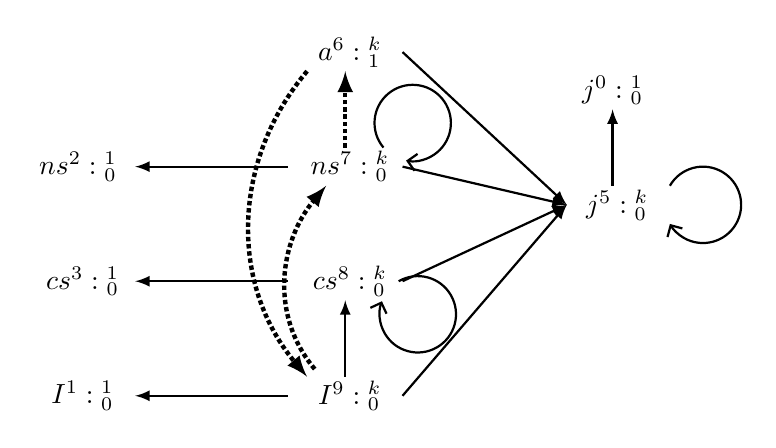
\begin{tikzpicture}[scale=\textwidth/25cm,samples=200]
% Variables Initialization
\draw[] (-7, 1) circle (0pt) node{{ $I^1: {}^1_{0}$}};
\draw[] (-7, 7) circle (0pt) node{{$ns^2: {}^{1}_{0}$}};
\draw[] (-7, 4) circle (0pt) node{{ $cs^3: {}^{1}_{0}$}};
% Variables Inside the Loop
     \draw[] (0, 10) circle (0pt) node{{ $a^6: {}^{k}_{1}$}};
     \draw[] (0, 7) circle (0pt) node{{ $ns^7: {}^{k}_{0}$}};
     \draw[] (0, 4) circle (0pt) node{{ $cs^8: {}^{k}_{0}$}};
     \draw[] (0, 1) circle (0pt) node{{ $I^9: {}^{k}_{0}$}};
     % Counter Variables
     \draw[] (7, 9) circle (0pt) node {{$j^0: {}^{1}_{0}$}};
     \draw[] (7, 6) circle (0pt) node {{ $j^5: {}^{k}_{0}$}};
     %
     % Value Dependency Edges:
     \draw[ thick, -latex,] (0, 1.5)  -- (0, 3.5) ;
     \draw[ ultra thick, -latex, densely dotted,] (0, 7.5)  -- (0, 9.5) ;
     \draw[ thick, -Straight Barb] (1.4, 4) arc (120:-200:1);
     \draw[ thick, -Straight Barb] (8.5, 6.5) arc (150:-150:1);
     \draw[ thick, -Straight Barb] (1, 7.5) arc (220:-100:1);
     \draw[ thick, -latex] (7, 6.5)  -- (7, 8.5) ;
     % Value Dependency Edges on Initial Values:
     \draw[ thick, -latex,] (-1.5, 1)  -- (-5.5, 1) ;
     \draw[ thick, -latex,] (-1.5, 4)  -- (-5.5, 4) ;
     \draw[ thick, -latex,] (-1.5, 7)  -- (-5.5, 7) ;
     %
     \draw[ ultra thick, -latex, densely dotted,] (-1, 9.5)  to  [out=-130,in=130]  (-1, 1.5);
     \draw[ ultra thick, -latex, densely dotted,] (-0.8, 1.7)  to  [out=-230,in=230]  (-0.5, 6.5);
     % Control Dependency
    %  \draw[ thick,-latex] (1.5, 7)  -- (4, 9) ;
    %  \draw[ thick,-latex] (1.5, 4)  -- (4, 9) ;
     \draw[ thick,-latex] (1.5, 7)  -- (5.8, 6) ;
     \draw[ thick,-latex] (1.5, 4)  -- (5.8, 6) ;
     \draw[ thick,-latex] (1.5, 1)  -- (5.8, 6) ;
     \draw[ thick,-latex] (1.5, 10)  -- (5.8, 6) ;
     \end{tikzpicture}
     \caption{}
        \end{centering}
        \end{subfigure}
    \vspace{-0.4cm}
    \caption{(a) The simplified multiple rounds example (b) The program-based dependency graph from $\THESYSTEM$}
    \vspace{-0.5cm}
    \label{fig:multi_graphs}
\end{figure}
%
\end{example}

\input{examples/linearRegressionGD}
\input{examples/multipleRoundsOdd}
\input{examples/multipleRoundsSingle}
% \input{examples/multipleRoundsSingleAccurate}

% \section{ \todo{Integrated into sections above} The Program Analysis Framework Improvement}
% \section{Adaptivity Analysis Refinement via Execution-Based Analysis}
\label{sec:refine-exe}
%
The program's adaptivity in the formal model through the execution-based analysis,
% which we define over the program's execution-based dependency graph from the dynamic 
% analysis 
in Definition~\ref{def:trace_adapt}, isn't precise enough w.r.t. the intuitive adaptivity rounds.
It comes across an over-approximation 
% on the program's
%  intuitive adaptivity rounds.
% It is 
resulted from difference between its Dependency Depth analysis and the \emph{variable may-dependency} definition.
It occurs when the weight is computed over the traces different from the traces used in 
witness the \emph{variable may-dependency} relation.
As shown in the Example~\ref{ex:multipleRoundSingle_example}.
\input{examples/multipleRoundsSingle}
%%
% \subsection{ Methodology}
% \label{sec:refine-exe-analysis}
% % In terms of techniques, our work relies on ideas from both static analysis and dynamic analysis. 
We discuss closely related work in both areas.



\subsection{Language Extension}
\label{subsec:refine-exe-language}
In this chapter, we formally introduce the language we will focus on for writing data analyses.  
This is a simple loop language with some primitives for calling queries. 
After defining the syntax of the language and showing an example, we will define its trace-based operational semantics. 
This is the main technical ingredient we will use to define the program's adaptivity.

%
%
\paragraph{Syntax Extension}
\[
\begin{array}{llll}
\mbox{Arithmetic Operators} 
& \oplus_a & ::= & + ~|~ - ~|~ \times 
%
~|~ \div ~|~ \max ~|~ \min\\  
% ~|~ \div \\  
\mbox{Boolean Operators} 
& \oplus_b & ::= & \lor ~|~ \land
\\
%
\mbox{Relational Operators} 
& \sim & ::= & < ~|~ \leq ~|~ == 
\\  
%
\mbox{Arithmetic Expression} 
& \aexpr & ::= & 
n ~|~ {x} ~|~ \aexpr \oplus_a \aexpr  
 ~|~ \elog \aexpr  ~|~ \esign \aexpr
\\
%
\mbox{Boolean Expression} & \bexpr & ::= & 
%
\etrue ~|~ \efalse  ~|~ \neg \bexpr
 ~|~ \bexpr \oplus_b \bexpr
%
~|~ \aexpr \sim \aexpr 
\\
%
\mbox{Expression} & \expr & ::= & v ~|~ \aexpr ~|~ \bexpr ~|~ [\expr, \dots, \expr]
\\  
%
\mbox{Value} 
& v & ::= & { n ~|~ \etrue ~|~ \efalse ~|~ [] ~|~ [v, \dots, v]}  
\\ 
&&&
\highlight
{
~|~ (r, x_1, \ldots, x_n) := c
}
\\
%
\mbox{Query Expression} 
& {\qexpr} & ::= 
& { \qval ~|~ \aexpr ~|~ \qexpr \oplus_a \qexpr ~|~ \chi[\aexpr]} 
\\
%
\mbox{Query Value} & \qval & ::= 
& {n ~|~ \chi[n] ~|~ \qval \oplus_a  \qval ~|~ n \oplus_a  \chi[n]
    ~|~ \chi[n] \oplus_a  n}
\\
% \\%
\mbox{Label} 
& l & ::= & (n \in \mathbb{N} \cup \{\lin, \lex\}) ~|~ (l, n)
\\ 
%
\mbox{Labeled Command} 
& {c} & ::= &  
\clabel{\assign{x}{\expr}}^l 
~|~ \clabel{\assign{x}{\query(\qexpr)}}^l
~|~  \clabel{\eskip}^l
~|~ \ewhile \clabel{\bexpr}^{l} \edo {c}
~|~ \eif(\clabel{\bexpr}^{l} , {c}, {c}) 
\\ 
&&&
\highlight
{
~|~ \clabel{\efun}^l: x(r, x_1, \ldots, x_n) := c
~|~ \clabel{\assign{x}{\ecall(x, e_1, \ldots, e_n)}}^l
}
~|~ {c};{c}  
\\ 
% \\
\mbox{Event} 
& \event & ::= & 
    ({x}, l, v, \bullet) ~|~ ({x}, l, v, \qval)  ~~~~~~~~~~~ \mbox{Assignment Event} \\
&&& ~|~(\bexpr, l, v, \bullet)   ~~~~~~~~~~~~~~~~~~~~~~~~~~~~~~~~~~ \mbox{Testing Event}
\\
% &&& \text{\mg{I think it would be better to use quadruples for events, where the}}\\
% &&& \text{\mg{first element is either a variable or a boolean expression and }}\\
% &&& \text{\mg{the last is either a query value or some default value $\bullet$}}\\
%
% \mbox{Trace} & \trace
% & ::= & \cdot | \trace \cdot \event | \trace \tracecat \trace 
% \\
%
% \mbox{Trace} & \trace
% & ::= & [] ~|~ \event:: \trace ~|~ \trace \tracecat \trace  \\
\mbox{Trace} & \trace
& ::= & [] ~|~ \trace :: \event\\
% &&& \text{\mg{I don't understand why you need both :: and ++ as constructors.}}\\
% &&& \text{\jl{Because append is to the left but we are adding element to the left in the OS}}\\
% &&& \text{\jl{I was too sticky to the convention, it is a good idea to append to the left and just use $::$}}
% %
% \mbox{Event Signature} & \sig
% & ::= & (x, l, n) | (x, l, n, \query) | (b, l, n)
% \\
% %
\end{array}
\]
% \todo{change trace notation into list, and update corresponding operator nations}
% \\
% \wqside{"$\cdot$" has two meanings? empty, delimit. Trace is list of event?}
We use following notations to represent the set of corresponding terms:
\[
\begin{array}{lll}
\mathcal{VAR} & : & \mbox{Set of Variables}  
\\ 
%
\mathcal{VAL} & : & \mbox{Set of Values} 
\\ 
%
\mathcal{QVAL} & : & \mbox{Set of Query Values} 
\\ 
%
\cdom & : & \mbox{Set of Commands} 
\\ 
%
\eventset  & : & \mbox{Set of Events}  
\\
%
\eventset^{\asn}  & : & \mbox{Set of Assignment Events}  
\\
%
\eventset^{\test}  & : & \mbox{Set of Testing Events}  
\\
%
\ldom  & : & \mbox{Set of Labels}  
\\
%%
\mathcal{VAL}  & : & \mbox{Set of Labeled Variables}  
\\
%%
\dbdom  & : & \mbox{{Set of Databases}} 
\\
%
{\mathcal{T}} & : & \mbox{Set of Traces}
\\
%
\mathcal{T}_0(c) & : & \mbox{Set of Initial Traces, where all the input variables of the program $c$ are initialized.
}
\\
%
% \qdom = {[-1,1]} & : & \mbox{{Domain of Query Results}}\\
\qdom & : & \mbox{{Domain of Query Results}}\\
% &&\text{\mg{I don't think you need to hard code [-1,1] here}}\\
\end{array}
\]
%
%
%
Environment $ \env : {\mathcal{T}}  \to \mathcal{VAR} \to \mathcal{VAL} \cup \{\bot\}$
% \mgside{The following definition is missing one case, also it is better to say that $y\neq x$.}
% \[
% \begin{array}{lll}
% \env(\trace  \tracecat [(x, l, v, \cdot)]) x \triangleq v
% &
% \env(\trace \tracecat [(y, l, v, \cdot)]) x \triangleq \env(\trace) x, y \neq x
% &
% \env(\trace \tracecat [(b, l, v, \cdot)]) x \triangleq \env(\trace) x
% \\
% \env(\trace \tracecat [(x, l, v, \qval)]) x \triangleq v
% &
% \env(\trace \tracecat [(y, l, v, \qval)]) x \triangleq \env(\trace) x, y \neq x
% &
% \env({[]} ) x \triangleq \bot
% \end{array}
% \]
\[
\begin{array}{lll}
\env(\trace  \traceadd (x, l, v, \bullet)) x \triangleq v
&
\env(\trace \traceadd (y, l, v, \bullet)) x \triangleq \env(\trace) x, y \neq x
&
\env(\trace \traceadd (b, l, v, \bullet)) x \triangleq \env(\trace) x
\\
\env(\trace \traceadd (x, l, v, \qval)) x \triangleq v
&
\env(\trace \traceadd (y, l, v, \qval)) x \triangleq \env(\trace) x, y \neq x
&
\env({[]} ) x \triangleq \bot
\end{array}
\]
%
%
% \subsection{Trace-based Operational Semantics for Language \mg{What is ``Language''?}}
\paragraph{{Trace-based Operational Semantics Extension}}
The trace based operational semantics rules are extended with the 
function procedure call, defined in Figure \ref{fig:os_extend}.
%
\begin{figure}
{
\begin{mathpar}
\boxed{
\mbox{Command $\times$ Trace}
\xrightarrow{}
\mbox{Command $\times$ Trace}
}
\and
\boxed{\config{{c, \trace}}
\xrightarrow{} 
\config{{c',  \trace'}}
}
\\
\inferrule
{
\empty
}
{
\config{\clabel{\eskip}^l,  \trace } 
\xrightarrow{} 
\config{\clabel{\eskip}^l, \trace}
}
~\textbf{skip}
%
\and
%
\inferrule
{
\event = ({x}, l, v, \bullet)
}
{
\config{[\assign{{x}}{\aexpr}]^{l},  \trace } 
\xrightarrow{} 
\config{\clabel{\eskip}^l, \trace \traceadd \event}
}
~\textbf{assn}
%
\and
%
{
\inferrule
{
 \config{\trace, \qexpr }\qarrow \qval
 \and 
\query(\qval) = v
\and 
\event = ({x}, l, v, \qval)
}
{
\config{{[\assign{x}{\query(\qexpr)}]^l, \trace}}
\xrightarrow{} 
\config{{\clabel{\eskip}^l,  \trace \traceadd \event} }
}
~\textbf{query}
}
%
\and
%
\inferrule
{
  \config{\trace, b} \barrow \etrue
 \and 
 \event = (b, l, \etrue, \bullet)
}
{
\config{{\ewhile [b]^{l} \edo c, \trace}}
\xrightarrow{} 
\config{{
c; \ewhile [b]^{l} \edo c,
\trace \traceadd \event}}
}
~\textbf{while-t}
%
%
\and
%
\inferrule
{
  \config{\trace, b} \barrow \efalse
 \and 
 \event = (b, l, \efalse, \bullet)
}
{
\config{{\ewhile [b]^{l}, \edo c, \trace}}
\xrightarrow{} 
\config{{
  \clabel{\eskip}^l,
\trace \traceadd \event}}
}
~\textbf{while-f}
%
%
\and
%
%
\inferrule
{
\config{{c_1, \trace}}
\xrightarrow{}
\config{{c_1',  \trace'}}
}
{
\config{{c_1; c_2, \trace}} 
\xrightarrow{} 
\config{{c_1'; c_2, \trace'}}
}
~\textbf{seq1}
%
\and
%
\inferrule
{
  \config{{c_2, \trace}}
  \xrightarrow{}
  \config{{c_2',  \trace'}}
}
{
\config{{\clabel{\eskip}^l; c_2, \trace}} \xrightarrow{} \config{{ c_2', \trace'}}
}
~\textbf{seq2}
%
\and
%
%
\inferrule
{
  \config{\trace, b} \barrow \etrue
 \and 
 \event = (b, l, \etrue, \bullet)
}
{
 \config{{
\eif([b]^{l}, c_1, c_2), 
\trace}}
\xrightarrow{} 
\config{{c_1, \trace \traceadd \event}}
}
~\textbf{if-t}
%
\and
%
\inferrule
{
 \config{\trace, b} \barrow \efalse
 \and 
 \event = (b, l, \efalse, \bullet)
}
{
\config{{\eif([b]^{l}, c_1, c_2), \trace}}
\xrightarrow{} 
\config{{c_2, \trace \traceadd \event}}
}
~\textbf{if-f}
% %
\and
%
\highlight{
\inferrule
{
 c' = (c)^{+n}
 \and 
 \event = (f, l, (r, x_1, \ldots, x_n) := c', \bullet)
}
{
\config{{
  [\efun]^l: f(r, x_1, \ldots, x_n) := c, \trace}}
\xrightarrow{} 
\config{{\clabel{\eskip}^l, \trace \traceadd \event}}
}
~\textbf{fun-def}
%
}
\\
\highlight{
%
\inferrule
{
  \config{ \trace, f} \earrow (r, x_1, \ldots, x_n) := c
\and 
\config{{
  \clabel{\assign{x_1}{e_1}}^{(l, 1)}; \ldots;
  \clabel{\assign{x_n}{e_n}}^{(l, n)}, \trace}} 
  \xrightarrow{}^* 
  \config{{\clabel{\eskip}^{(l, n)}, \trace_1}}
  \\ 
  \config{{\clabel{c}^{(l)}, \trace_1}}
  \xrightarrow{}^* 
  \config{{\clabel{\eskip}^{l}, \trace'}}
  \and
  \config{\trace', r } \earrow v
  \and
 \event = (x, l, v, \bullet)
}
{
\config{{
  \clabel{\assign{x}{\ecall(f, e_1, \ldots, e_n)}}^l, \trace}}
\xrightarrow{} 
\config{{\clabel{\eskip}^l, \trace' :: \event}}
}
~\textbf{fun-call}
}
%
\end{mathpar}
}
% \end{subfigure}
    \caption{Trace-based Operational Semantics for Language.}
    \label{fig:os_extend}
\end{figure}
%
\\
\highlight{
  \begin{defn}[Label Increase]
    \label{def:label_inc}  
    Label Increase $ + : {\ldom \to \mathbb{N} \to \ldom}$, increase a label $l$ by a natural number $n$:
\[
    n + n' \triangleq n'' ~ n, n' \in \mathbb{N} \land \config{[], n + n'} \aarrow n''
   \qquad (l, n) + n' \triangleq (l + n', n'') ~ n, n' \in \mathbb{N} \land \config{[], n + n'} \aarrow n''
   \]
\end{defn}
The case of $(l, n) + n'$ will never happen during evaluation.
By Operational semantics, the only place the label increase is in rule \textbf{fun-def},
$c' = (c)^{+n}$, where $c$ is the function body.
By the rule \textbf{fun-call}, and the label augment in Definition~\ref{def:comlabel_aug}, the function body $c$ will never be augmented.
%
\begin{defn}[Command Label Increase] 
  \label{def:comlabel_inc}
Command Label Increase $ {(\cdot)}{}^{+n} : {\cdom \to \cdom}$, increase the label in command by $n$.
\[
\begin{array}{ll}
  (\clabel{\assign{x}{\expr}}^l){}^{+n} & \triangleq \clabel{\assign{x}{\expr}}^{l + n}\\
(\clabel{\assign{x}{\query(\qexpr)}}^l)^{+n} & \triangleq \clabel{\assign{x}{\query(\qexpr)}}^{l + n}\\
(\clabel{\eskip}^l)^{+n} & \triangleq \clabel{\eskip}^{l + n}\\
(\ewhile \clabel{\bexpr}^{l} \edo {c'})^{+n} & \triangleq \ewhile \clabel{\bexpr}^{l+n} \edo {(c')^{+n}}\\
(\eif(\clabel{\bexpr}^{l} , {c_1}, {c_2}))^{+n}  & \triangleq \eif(\clabel{\bexpr}^{l+n} , {(c_1)^{+n}}, {(c_2)^{+n}})\\
% (\clabel{\efun}^l: x(r^l, x_1, \ldots, x_n) := c)^{+n} & \triangleq \clabel{\efun}^{l + n}: x(r^l, x_1, \ldots, x_n) := (c)^{+n} \\
(\clabel{\efun}^l: x(r^l, x_1, \ldots, x_n) := c)^{+n} & \triangleq \clabel{\efun}^{l + n}: x(r^l, x_1, \ldots, x_n) := c \\
(\clabel{\assign{x}{\ecall(x, e_1, \ldots, e_n)}}^l)^{+n} & \triangleq \clabel{\assign{x}{\ecall(x, e_1, \ldots, e_n)}}^{l + n}\\
({c_1};{c_2})^{+n} &  \triangleq {(c_1)}^{+n};{(c_2)}^{+n}
\end{array}
\]
\end{defn}
%
\begin{defn}[Command Label Augment] 
  \label{def:comlabel_aug}
  Command Label Augment $ \clabel{\cdot}^{l} : {\cdom \to \cdom}$, augment the label in command with a label $l$ 
in order to record the calling site.
\[
\begin{array}{ll}
  \clabel{\clabel{\assign{x}{\expr}}^{l'}}{}^{l} & \triangleq \clabel{\assign{x}{\expr}}^{(l, l')}\\
  \clabel{\clabel{\assign{x}{\query(\qexpr)}}^{l'}}^{l} & \triangleq \clabel{\assign{x}{\query(\qexpr)}}^{(l, l')}\\
  \clabel{\clabel{\eskip}^{l'}}^{l} & \triangleq \clabel{\eskip}^{(l, l')}\\
  \clabel{\ewhile \clabel{\bexpr}^{l'} \edo {c'}}^{l} & \triangleq \ewhile \clabel{\bexpr}^{(l, l')} \edo {(c')^{l}}\\
  \clabel{\eif(\clabel{\bexpr}^{l'} , {c_1}, {c_2})}^{l}  & \triangleq \eif(\clabel{\bexpr}^{(l, l')} , {(c_1)^{l}}, {(c_2)^{l}})\\
  \clabel{\clabel{\efun}^{l'}: x(r^l, x_1, \ldots, x_n) := c}^{l} & \triangleq \clabel{\efun}^{(l, l')}: x(r^l, x_1, \ldots, x_n) := c \\
  \clabel{\clabel{\assign{x}{\ecall(x, e_1, \ldots, e_n)}}^{l'}}^{l} & \triangleq \clabel{\assign{x}{\ecall(x, e_1, \ldots, e_n)}}^{(l, l')}\\
  \clabel{{c_1};{c_2}}^{l} &  \triangleq \clabel{c_1}^{l};\clabel{c_2}^{l}
\end{array}
\]
\end{defn}
}

\subsection{Execution-Based Data Dependency Analysis Refinement}
\label{subsec:refine-exe-datadep}
\paragraph{Challenge}
\label{para:exe-dep-challenge}
In the data analysis model the programming framework supports, 
%  an \emph{analyst} asks a sequence of queries to the mechanism, and receives the answers to these queries from the mechanism. In this model, the adaptivity I are interested in is the length of the longest sequence of such adaptively chosen queries, among all the queries the data analyst asks. 
  I define that a query is adaptively chosen when it is affected by answers of previous queries. The next thing is to decide how do I define whether one query is "affected" by previous answers, with the limited information I have? As a reminder, 
 when the analyst asks a query, the only known information will be the answers to previous queries and the current execution trace of the program.


There are two possible situations that a query will be "affected",  
either when the query expression directly uses the results of previous queries (data dependency), or when the control flow of the program with respect to a query (whether to ask this query or not) depends on the results of previous queries (control flow dependency).
% As a first step, I give a definition of when one query may depend on a previous query, which is supposed to consider both control dependency and data dependency. We first look at two possible candidates:
% \begin{enumerate}
%     \item One query may depend on a previous query if and only if a change of the answer to the previous query may also change the result of the query.
%     \item One query may depend on a previous query if and only if a change of the answer to the previous query may also change the appearance of the query.
% \end{enumerate}


Since the results of previous queries can be stored or used in variables
which aren't associated to the query request,
it is necessary to track the dependency between queries, through all the program's variables.
In the meantime, the trace-based operational semantics tracks the information,
distinguishing variables which are assigned with query requests.
% and then I can distinguish variables which are assigned with query requests.
In this way, the \emph{may-dependency} relation between queries can be recovered through 
the \emph{may-dependency} relation over all the program's variables.
According to this, I focus on the analysis on the variable \emph{may-dependency} relation in the following of this section.

I give a definition of when one variable \emph{may-depend} on a previous variable with two candidates.
{
\begin{enumerate}
    \item One variable may depend on a previous variable if and only if a change of the value assigned to the previous variable may also change the value assigned to the variable.
    \item One variable may depend on a previous variable if and only if a change of the value assigned to the previous variable may also change the appearance of the assignment command to this variable 
    % in\wq{during?} 
    during execution.
\end{enumerate}
}
%   The first candidate works well by witnessing the result of one query according to the change of the answer of another query. We can easily find that the two queries have nothing to do with each other in a simple example   

{   
% The first situations works well by witnessing the result assigned to variable 
% according to the change of the value assigned to another query. 
% We can easily find that the two queries have nothing to do with each other in a simple example 
% In the first one, by defining the dependency as
The first definition is defined as
% witnessing 
% the query expressions equivalence (or the value equality for non-query assignment )
the witness of a variation on the value assigned to the same variable through two executions,
% assigned to the same variable through two executions, 
according to the change of the value assigned to another variable in pre-trace.
% the situation of data-dependency works well. \wq{long sentence, make it short?}
In particular for query requests, the variation I observe is on the query value instead of on the query requesting results.
% We can find that two queries 
% % have nothing to do with each other in this simple example 
% % depends on each other\wq{not each other, one direction.} 
% satisfy this definition
In 
%this 
the simple program $c_1 =\assign{x}{\query(\chi[2])} ;\assign{y}{\query(\chi[3] + x)}$.
 %
 From our perspective, $\query(\chi[1])$ is different from $\query(\chi[2]))$. Informally, I think $\query(\chi[3] + x)$ may depend on the query $\query(\chi[2]))$, because equipped function of the former $\chi[3] + x$ may depend on the data stored in x assigned with the result of $\query(\chi[2]))$, according to this definition. }
%
% in this example: $c_1 = \assign{x}{\query(0)}; \assign{z}{\query(\chi[x])}$.
% This candidate definition works well 
Nevertheless, the first definition fails to catch control dependency because it just monitors the changes to a query, but misses the appearance of the query when the answers of its previous queries change. 
For instance, it fails to handle $
      c_2 = \assign{x}{\query(\chi[1])} ; \eif( x > 2 , \assign{y}{\query(\chi[2])}, \eskip )
   $, but the second definition can. However, it only considers the control dependency and misses the data dependency. 
  This reminds me to define a \emph{may-dependency} relation between labeled variables by combining the two definitions to capture the two situations.
%
%
% I define the According to the trace-based operational semantics,
%
\paragraph*{Value Difference on Traces}
%
\highlight{
  To define the \emph{may-dependency} relation on two labeled variables, I rely on the limited information at hand - the trace generated by the operational semantics. In this end, 
% So I first define some operations on the trace.
% In order to define the \emph{may-dependency} relation, 
Specifically, we need to be able to observe the difference of the values for each variable
through traces, i.e., through the events contained in traces.
Followed by this, it is necessary to give formal definition on observing this difference through traces.
Given the limitation of previous definition based on limited language,
I present the new definitions on observing the value difference as follows.
These new definitions help in formally capturing the intuitive \emph{adaptivity} precisely, concisely, and efficiently.}
%  in order to observe the evaluation variation in a different way, formally as follows.
\highlight{
\begin{defn}[Value Sequence $\seq(\trace, x^l)$]
  \label{def:vseq}
  \[
\begin{array}{l}
  \seq(\trace :: (x, l, v, \bullet), x^l) \triangleq \seq(\trace)::v  \qquad
  \seq(\trace :: (x, l, v, \qval), x^l) \triangleq \seq(\trace):: \qval \qquad
  \seq([]) \triangleq []\\
  \seq(\trace :: (y, j, \_, \_), x^l) \triangleq \seq(\trace) \quad y \neq x \lor j \neq l 
\end{array}
\]
\end{defn}
%
\begin{defn}[Difference Sequence $\sdiff(\trace_1, \trace_2, x^l )$]
  \label{def:diffseq}
  Let $ s_1 = \seq(\trace_1, x^l) \land s_2 = \seq(\trace_2, x^l)$ be the value sequence of $x^l$ 
  on $\trace_1$ and $\trace_2$, and $s^l$ be the sequence with longer length and $s^t$ the 
  shorter one,
  then their difference sequence is defined as follows,
  \[
    \sdiff(\trace_1, \trace_2, x^l) \triangleq
    \begin{array}{l}
      \{ (s^t[k], s^l[k]) ~|~ 
      % \land 
      % \land 
      s^t[k] \neq s^l[k], k = 0, \ldots, len(s^t)
      \}
      \\
      \cup 
      \{ (\cdot, s^l[k]) ~|~ 
      \len(s^t) \leq \len(s^l)k = len(s^t), \ldots \len(s^l)
      \}
    \end{array}
    \]
\end{defn}
}
\highlight{
  The new analysis compares the difference for all the
  query request evaluation, the non-query assignment evaluation, and the boolean evaluation.
  In this way, all the evaluation information related to the dependency is captured.
  Comparing to the previous works on formalizing adaptivity, which only observe the query difference,
  the new definitions help in analyzing and formalizing the adaptivity more precisely.
}
% A program $c$'s query variables is a subset of 
% its labeled variables, $\qvar(c) \subseteq \lvar(c)$. We have the operator $\tlabel : \mathcal{T} \to \ldom$, which gives the set of labels in every event belonging to the trace.
% Then I introduce a counting operator $\vcounter : \mathcal{T} \to \mathbb{N} \to \mathbb{N}$, 
% % \wq{which counts the occurrence of of a variable in the trace,} 
% which counts the occurrence of a labeled variable in the trace,
% whose behavior is defined as follows,
% \[
% \begin{array}{ll}
% \vcounter(\trace :: (\_, l, \_, \_), l ) \triangleq \vcounter(\trace, l) + 1
% &
% \vcounter(\trace  ::(b, l, v, \bullet), l) \triangleq \vcounter(\trace, l) + 1
% \\
% \vcounter(\trace  :: (x, l, v, \qval), l) \triangleq \vcounter(\trace, l) + 1
% &
% % \vcounter(\trace :: (\_, l', \_, \_), l ) \triangleq \vcounter(\trace, l), l' \neq l 
% % &
% \vcounter(\trace  :: (x, l', v, \bullet), l) \triangleq \vcounter(\trace, l), l' \neq l
% \\
% \vcounter(\trace  :: (b, l', v, \bullet), l) \triangleq \vcounter(\trace, l), l' \neq l
% &
% \vcounter(\trace  :: (x, l', v, \qval), l) \triangleq \vcounter(\trace, l), l' \neq l
% \\
% \vcounter({[]}, l) \triangleq 0
% \end{array}
% \]
  \paragraph{Event Dependency}
\todo{
 To define the \emph{may-dependency} relation on two labeled variables, I rely on the limited information at hand - the trace generated by the operational semantics. In this end, 
 I first define the \emph{may-dependency} between events, and use it as a foundation of the variable may-dependency relation.
\begin{defn}[Events Different up to Value ($\diff$)]
  Two events $\event_1, \event_2 \in \eventset$ are  \emph{Different up to Value}, 
  denoted as $\diff(\event_1, \event_2)$ if and only if:
  \[
    \begin{array}{l}
  \pi_1(\event_1) = \pi_1(\event_2) 
  \land  
  \pi_2(\event_1) = \pi_2(\event_2) \\
  \land  
  \big(
    (\pi_3(\event_1) \neq \pi_3(\event_2)
  \land 
  \pi_{4}(\event_1) = \pi_{4}(\event_2) = \bullet )
  % \qquad \qquad 
  \lor 
  (\pi_4(\event_1) \neq \bullet
  \land 
  \pi_4(\event_2) \neq \bullet
  \land 
  \pi_{4}(\event_1) \neq_q \pi_{4}(\event_2)) 
  \big)
  \end{array}
  \]
  \end{defn}
 %
 We compare two events by defining $\diff(\event_1, \event_2)$. We use $\qexpr_1 =_{q} \qexpr_2$ and $\qexpr_1 \neq_{q} \qexpr_2$ to notate query expression equivalence and in-equivalence, distinct from standard equality. A program $c$'s
%  , its 
 labeled variables 
%  and assigned variables are subsets of 
is a subset of
the labeled variables $\mathcal{LV}$, denoted by $\lvar(c) \in \mathcal{P}(\mathcal{VAR} \times \mathcal{L}) \subseteq \mathcal{LV}$.
% annotated by a label. 
% We use  
%$\mathcal{LVAR} = \mathcal{VAR} \times \mathcal{L} $ 
% $\mathcal{LV}$ represents the universe of all the labeled variables and 
% $\avar(c) \in \mathcal{P}(\mathcal{VAR} \times \mathbb{N}) \subset \mathcal{LV}$ and 
% $\lvar(c) \in \mathcal{P}(\mathcal{VAR} \times \mathcal{L}) \subseteq \mathcal{LV}$ for them. 
We also define the set of query variables for a program $c$, $\qvar: \cdom \to 
\mathcal{P}(\mathcal{LV})$.
\\
A program $c$'s query variables is a subset of 
its labeled variables, $\qvar(c) \subseteq \lvar(c)$. We have the operator $\tlabel : \mathcal{T} \to \ldom$, which gives the set of labels in every event belonging to the trace.
Then I introduce a counting operator $\vcounter : \mathcal{T} \to \mathbb{N} \to \mathbb{N}$, 
% \wq{which counts the occurrence of of a variable in the trace,} 
which counts the occurrence of a labeled variable in the trace,
whose behavior is defined as follows,
\[
\begin{array}{ll}
\vcounter(\trace :: (\_, l, \_, \_), l ) \triangleq \vcounter(\trace, l) + 1
&
\vcounter(\trace  ::(b, l, v, \bullet), l) \triangleq \vcounter(\trace, l) + 1
\\
\vcounter(\trace  :: (x, l, v, \qval), l) \triangleq \vcounter(\trace, l) + 1
&
% \vcounter(\trace :: (\_, l', \_, \_), l ) \triangleq \vcounter(\trace, l), l' \neq l 
% &
\vcounter(\trace  :: (x, l', v, \bullet), l) \triangleq \vcounter(\trace, l), l' \neq l
\\
\vcounter(\trace  :: (b, l', v, \bullet), l) \triangleq \vcounter(\trace, l), l' \neq l
&
\vcounter(\trace  :: (x, l', v, \qval), l) \triangleq \vcounter(\trace, l), l' \neq l
\\
\vcounter({[]}, l) \triangleq 0
\end{array}
\]
% The full definitions of these above operators can be found in the appendix.
\begin{defn}[Event May-Dependency].
\label{def:event_dep}
\\ 
  An event $\event_2$ is in the \emph{event may-dependency} relation with an assignment
  event $\event_1 \in \eventset^{\asn}$ in a program ${c}$
  with a hidden database $D$ and a trace $\trace \in \mathcal{T}$ denoted as 
  %
  $\eventdep(\event_1, \event_2, [\event_1 ] \tracecat \trace \tracecat [\event_2], c, D)$, iff
  %
  \[
    \begin{array}{l}
  \exists \vtrace_0,
  \vtrace_1, \vtrace' \in \mathcal{T},\event_1' \in \eventset^{\asn}, {c}_1, {c}_2  \in \cdom  \sthat
  \diff(\event_1, \event_1') \land 
      \\ \quad
      (
        \exists  \event_2' \in \eventset \sthat 
    \left(
    \begin{array}{ll}   
   & \config{{c}, \vtrace_0} \rightarrow^{*} 
  \config{{c}_1, \vtrace_1 \tracecat [\event_1]}  \rightarrow^{*} 
    \config{{c}_2,  \vtrace_1 \tracecat [\event_1] \tracecat \vtrace \tracecat [\event_2] } 
    % 
   \\ 
   \bigwedge &
    \config{{c}_1, \vtrace_1 \tracecat [\event_1']}  \rightarrow^{*} 
    \config{{c}_2,  \vtrace_1 \tracecat[ \event_1'] \tracecat \vtrace' \tracecat [\event_2'] } 
  \\
  \bigwedge & 
  \diff(\event_2,\event_2' ) \land 
  \vcounter(\vtrace, \pi_2(\event_2))
  = 
  \vcounter(\vtrace', \pi_2(\event_2'))\\
  \end{array}
  \right)
  \\ \quad
  \lor 
  \exists \vtrace_3, \vtrace_3'  \in \mathcal{T}, \event_b \in \eventset^{\test} \sthat 
  \\ \quad
  \left(
  \begin{array}{ll}   
    & \config{{c}, \vtrace_0} \rightarrow^{*} 
      \config{{c}_1, \vtrace_1 \tracecat [\event_1]}  \rightarrow^{*} 
      \config{c_2,  \vtrace_1 \tracecat [\event_1] \tracecat \trace \tracecat [\event_b] \tracecat  \trace_3} 
    \\ 
    \bigwedge &
    \config{{c}_1, \vtrace_1 \tracecat [\event_1']}  \rightarrow^{*} 
    \config{c_2,  \vtrace_1 \tracecat [\event_1'] \tracecat \trace' \tracecat [(\neg \event_b)] \tracecat \trace_3'} 
    \\
    \bigwedge &  \tlabel_{\trace_3} \cap \tlabel_{\trace_3'} = \emptyset
     \land \vcounter(\trace', \pi_2(\event_b)) = \vcounter(\trace, \pi_2(\event_b)) 
    %   \land \event_2 \eventin \trace_3
    % \land \event_2 \not\eventin \trace_3'
    \land \event_2 \in \trace_3
    \land \event_2 \not\in \trace_3'
  \end{array}
  \right)
  )
\end{array}
   \]
% , where ${\tt label}(\event_2) = \pi_2(\event_2)$.
  %  
%
\end{defn}
% \todo{add explnanation}
% \jl{
Our event \emph{may-dependency} relation of 
two events $\event_1 \in \eventset^{\asn}$ and $\event_2 \in \eventset$, 
for a program $c$ and hidden database $D$ is w.r.t to
a trace $[\event_1 ] \tracecat \trace \tracecat [\event_2]$.
The $\event_1 \in \eventset^{\asn}$ is an assignment event because only a change on an assignment event will affect the execution trace, according to our operational semantics.
In order to observe the changes of $\event_2$ under the modification of $\event_1$, this trace 
$[\event_1 ] \tracecat \trace \tracecat [\event_2]$
starts with $\event_1$ and ends with $\event_2$.
% }
{The \emph{may-dependency} relation considers both the value dependency and value control dependency as discussed in 
analysis challenges in Paragraph~\ref{para:exe-dep-challenge}. The relation can be divided into two parts naturally in Definition~\ref{def:event_dep} (line $2-4$, $5-8$ respectively, starting from line $1$). The idea of the event $\event_1$ may depend on $\event_2$ can be briefly described:
I have one execution of the program as reference (See line $2$ and $6$, for the two kinds of dependency). 
When the value assigned to the 
% first variable 
first variable in $\event_1$ is modified, the reference trace $\trace_1 \tracecat [\event_1]$ is modified correspondingly to $\trace_1 \tracecat [\event_1']$.
We use $\diff(\event_1, \event_1')$ at line $1$ to express this modification, which guarantees that $\event_1$ and $\event_1'$ only differ in their assigned values and are equal on variable name and label. We perform a second run of the program by continuing the execution of the same program from the same execution point, 
but with the modified trace $\trace_1 \tracecat [\event_1']$ (See line $3$, $7$). 
The expected may dependency will be caught by observing two different possible changes (See line $4, 8$ respectively) when comparing the second execution with the reference one (similar definitions as in \cite{Cousot19a}). 
\\
% \wq{
% In the first situation, I are witnessing 
In the first part (line $2-4$ of Definition~\ref{def:event_dep}), I witness
% that the value assigned to the second variable in $\event_2$
the appearance of $\event_2'$ in the second execution, and
% a variation in $\event_2$, which changes into $\event_2'$.
a variation between $\event_2$ and $\event_2'$ on their values.
% changes in $\event_2'$.
% \jl{
We have special requirement $\diff(\event_2, \event_2')$, which guarantees that they
have the same variable name and label but only differ 
% % in their assigned value. 
in their evaluated values.
% assigned to the same variable. 
In particularly for queries, if $\event_2$ and $\event_2'$ are 
% query assignment events, then 
generated from query requesting, then $\diff(\event_2, \event_2')$ guarantees that
they differ in their query values rather than the 
% query requesting value. 
query requesting results. 
Additionally, in order to handle multiple occurrences of the same event through iterations of the while loop,
 where  $\event_2$ and $\event_2'$ could be 
in different while loops,
I restrict the same occurrence of $\event_2$'s label in $\trace$ from the first execution with  the occurrence of $\event_2'$'s label in $\trace'$ from the second execution,
through $\vcounter(\vtrace, \pi_2(\event_2))
= 
\vcounter(\vtrace', \pi_2(\event_2'))$ at line $4$.
% }
% }
\\
% \wq{
In the second part (line $5-8$ of Definition~\ref{def:event_dep}), I 
% are witnessing 
witness
the disappearance of $\event_2$ through observing the change of a testing event $\event_b$.
% In order to change the appearance of 
% % and event, the command that generating $\event_2$ must not be executed in 
% 5yhan event, 
To witness
the disappearance, the command that generates $\event_2$ must not be executed in 
the second execution. 
The only way to control whether a command will be executed, is through the change of a guard's 
evaluation result in an if or while command, which generates a testing event $\event_b$ in the first place.
So I observe when
$\event_b$ changes into $\neg \event_b$ in the second execution firstly, 
whether it follows with the disappearance of $\event_2$ in the second trace. We restrict the occurrence of $\event_b$'s label in the two traces being the same
}
% s to the occurrence times of $\event_2'$'s label in the second trace,
through $\vcounter(\trace', \pi_2(\event_b)) = \vcounter(\trace, \pi_2(\event_b))$ to handle the while loop.
% changes in $\event_2'$, have the same variable and label and only differ in their assigned value. 
Again, for queries, I observe the disappearance based on the query value equivalence.
% if $\event_2$ and $\event_2'$ are query assignment events, then 
% they differ in their query value rather than the assigned value. 
% }
%
% \mg{I don't understand this explanation. What are the ``assignment commands associated to the two labelled variables''}
% \jl{revised but need more think}
% Explanation: 
}
\paragraph*{Variable Dependency}
{Considering 
% a program's all possible executions 
all events generated during a program's executions
under an initial trace,
% among all events generated during these executions
% and the variables and labels of these events are 
% corresponding to the two labeled variables,
% evaluations of the assignment commands associated to the two labelled variables respectively, 
as long as there is one pair of events satisfying the \emph{event may-dependency} relation in Definition~\ref{def:event_dep}, 
 I say the two 
related
variables satisfy the \emph{variable may-dependency} relation, in Definition~\ref{def:var_dep}.
}
\begin{defn}[Variable May-Dependency]
    \label{def:var_dep}
\highlight{
    A labeled variable $y^j \in \lvar(c)$ is in the \emph{may-dependency} relation with another
    labeled variable $x^i \in \lvar(c)$ in a program ${c}$, w.r.t. an initial trace $\trace_0 \in \mathcal{T}_0(c)$
    and two witness traces $\trace_1, \trace_2 \in \mathcal{T}$,
    denoted as 
    %
    $\dep(x^i, y^j, \trace_1, \trace_2, \trace_0, {c})$, if an only if
    \[
      \begin{array}{l}
    \exists 
    D \in \dbdom, 
    \trace_0' \in \mathcal{T} \sthat
    (\forall z \neq x \sthat   \env(\trace_0 ) z =   \env(\trace_0') z )
    \\ \quad \land 
     \config{{c}, \vtrace_0} \rightarrow^{*} 
      \config{\clabel{\eskip}^l, \vtrace_0  \tracecat \trace_1 } 
      \land 
      % \config{{c}_1, \vtrace_0' \tracecat [\event_1']}  \rightarrow^{*} 
      % \config{\clabel{\eskip}^l,  
      % \vtrace_0' \tracecat [\event_1] \tracecat \trace_2 }   
      \config{{c}, \vtrace_0'} \rightarrow^{*} 
      % \config{{c}_1, \vtrace_0' \tracecat [\event_1]}  \rightarrow^{*} 
        \config{\clabel{\eskip}^l, \vtrace_0'  \tracecat \trace_2} 
      \land 
        \sdiff(\trace_1, \trace_2, y^j ) \neq \emptyset
      \end{array}
    \]  
  }
    \end{defn}
    Specifically, I define the variables dependency relation over two witness traces and an initial trace. Comparing to 
    the previous \emph{may-dependency} definition, which quantifies overall possible execution traces, the alternative
    definition explicitly relies on two specific witness traces from execution.
    % \\
\highlight{This externalization of the two witness traces also helps in analyzing the dependency quantity through the same 
witness traces as the \emph{may-dependency} relation. 
In this way, the in-accuracy in formalizing the \emph{adaptivity}
is reduced further.}

% \begin{defn}[Variable May-Dependency].
%   \label{def:var_dep}
%   \\
%   A variable ${x}_2^{l_2} \in \lvar(c)$ is in the \emph{variable may-dependency} relation with another
%   variable ${x}_1^{l_1} \in \lvar(c)$ in a program ${c}$, denoted as 
%   %
%   $\vardep({x}_1^{l_1}, {x}_2^{l_2}, {c})$, if and only if.
% \[
%   \begin{array}{l}
% \exists \event_1, \event_2 \in \eventset^{\asn}, \trace \in \mathcal{T} , D \in \dbdom \sthat
% % (\pi_{1}{(\event_1)}, \pi_{2}{(\event_1)}) = ({x}_1, l_1)
% % \land
% % (\pi_{1}{(\event_2)}, \pi_{2}{(\event_2)}) = ({x}_2, l_2)
% \pi_{1}{(\event_1)}^{\pi_{2}{(\event_1)}} = {x}_1^{l_1}
% \land
% \pi_{1}{(\event_2)}^{\pi_{2}{(\event_2)}} = {x}_2^{l_2}% \\ \quad 
% \land 
% \eventdep(\event_1, \event_2, \trace, c, D) 
%   \end{array}
% \]  %
% \end{defn}
\highlight{\paragraph*{Improvements Analysis}
Comparing to previous works,
this new dependency definition is more precise and efficient.
% language and operational semantics design improves the expressiveness, efficiency, and the accuracy to a large extend.
\begin{itemize}
  %   \item \textbf{Improvements on Expressiveness}
  \item \textbf{Improvements on Accuracy}
  \\
  The accuracy is improved in the following senses.
  \\
  By Definition~\ref{def:vseq} and \ref{def:diffseq}, all the information related to the dependency is able to be observed.
  In this sense, the dependency can be analyzing more accurately.
  \\
  By Definition~\ref{def:var_dep}, 
  all the dependency information for variables is captured, including queries. 
  According to this, the adaptivity can be formalized more accurately.
\\
Moreover, the Definition~\ref{def:var_dep} externalized the witness traces. This externalization
helps in analyzing the dependency quantity precisely and improving the adaptivity formalization accordingly.
  %   \\
  % This language is extended over the standard while language. 
  % In this sense, it supports all the general data analysis.
  \item \textbf{Improvements on Efficiency}
  \\
  The efficiency improvements come from the language design, where the program evaluation efficiency is improved. 
  Then efficiency of this execution-based analysis is improved accordingly.
  \end{itemize}
  }
\paragraph*{Dependency Relation through The Two Rounds Example}
\begin{example}[Variable \emph{May-Dependency} Relation in The Two Rounds Data Analysis Example Program]
    In the same $\kw{towRounds(k)}$ example Program,    the analyst asks in total $k+1$ queries to the mechanism in two phases.
    %
    \[         \begin{array}{l}
      \kw{towRounds(k)} \triangleq \\
             \clabel{ \assign{a}{0}}^{0} ;
              \clabel{\assign{j}{k} }^{1} ;\\
              \ewhile ~ \clabel{j > 0}^{2} ~ \edo ~
              \Big(
               \clabel{\assign{x}{\query(\chi[j] \cdot \chi[k])} }^{3}  ;
               \clabel{\assign{j}{j-1}}^{4} ;
              \clabel{\assign{a}{x + a}}^{5}       \Big);\\
              \clabel{\assign{l}{\query(\chi[k]*a)} }^{6}
          \end{array}
          \]    %
    % Queries are of the form $q(e)$ where $e$ is an expression with a special variable $\chi$ representing a possible row. Mainly $e$ represents a function from $X$ to some domain $U$, for example $U$ could be $[-1,1]$ or $[0,1]$. This function characterizes the linear query I are interested in running. As an example, $x \leftarrow q(\chi[2])$ computes an approximation, according to the used mechanism, of the empirical mean of the second attribute, identified by $\chi[2]$. Notice that I don't materialize the mechanism but I assume that it is implicitly run when I execute the query. 
    % \jl{We use $\chi$ to abstract a possible row in the database and }
    % queries are of the form $\query(\qexpr)$, where $\qexpr$ is a special expression 
    In order to analysis the \emph{may-dependency} relation for variable 
    $x^3$ and $a^5$, I first generate the following execution trace with the initial trace
    $\trace_0 = [(k, in, 2, \bullet)]$ as follows,
   %   where $k$ is the 
   %  initial value of input variable $k$ given by user,
   %  we observe the execution trace as
   \\
    $
    \left[\begin{array}{l}
    % \trace_0 \tracecat
     (a, 0, 0, \bullet),
    (j, 1, 2, \bullet),
    (j>0, 2, \etrue, \bullet),
    (x, 3, v_1, \chi[2]*\chi[2]),
    (j, 4, 1, \bullet),
    (a, 5, v_1, \bullet),\\
    (j>0, 2, \etrue, \bullet),
    (x, 3, v_2, \chi[1]*\chi[2]),
    (j, 4, 0, \bullet),
    (a, 5, v_1 + v_2, \bullet),
    (j>0, 4, \efalse, \bullet),\\
    (l, 6, v_3, \chi[2]*( v_1 + v_2))
    \end{array} \right]
    $.
    \\
    We modify the value assigned to $x$ when evaluating the command $ \clabel{\assign{x}{\query(\chi[j] \cdot \chi[k])} }^{3}$
    in the first iteration.
    By manipulating the event in the trace, 
    the event $(x, 3, v_1, \chi[2]*\chi[2])$
    is modified into $(x, 3, v_1', \chi[2]*\chi[2])$ where $v_1 \neq v_1'$.
    Then, through executing the program from the execution point after executing line $3$, we observe another execution trace as follows,
    \\
    $
    \left[\begin{array}{l}
    % \trace_0 \tracecat
     (a, 0, 0, \bullet),
    (j, 1, 2, \bullet),
    (j>0, 2, \etrue, \bullet),
    \highlight{(x, 3, v_1', \chi[2]*\chi[2])},
    (j, 4, 1, \bullet),
    (a, 5, v_1, \bullet),\\
    (j>0, 2, \etrue, \bullet),
    (x, 3, v_2, \chi[1]*\chi[2]),
    (j, 4, 0, \bullet),
    \highlight{(a, 5, v_1' + v_2, \bullet),}
    (j>0, 4, \efalse, \bullet),\\
    (l, 6, v_3, \chi[2]*( v_1' + v_2))
    \end{array} \right]
    $.   
    \\
    In this trace, the event $(a, 5, v_1' + v_2, \bullet),$  is different from $(a, 5, v_1 + v_2, \bullet),$ in the first 
    trace.
    \\
    This change satisfies the Definition~\ref{def:event_dep}, so there exists the variable \emph{may-dependency} relation 
    between variable $x^3$ and $a^5$.
\end{example}

1. In the first stage of the execution-based analysis, 
I will give an alternative variable \emph{may-dependency} definition 
by referring to the analysis methodology in \cite{Cousot19a}.
\\
Specifically, I will define the variables dependency relation over two witness traces and an initial trace. Comparing to 
the existing \emph{may-dependency} definition, which quantifies overall possible execution traces, the alternative
definition explicitly relies on two specific witness traces from execution.
This externalization helps in analyzing the dependency quantity through the same 
witness traces as the \emph{may-dependency} relation. In this way, the over-approximation as illustrated above
can be reduced.

\subsection{Data Dependency Quantity Analysis Refinement}
\label{subsec:refine-exe-reachability}
% For a program $c$ I compute the reachability bound for every labeled variable overall $c$'s execution traces,
w.r.t. an initial trace as follows,
\[
  rb(x^l) \triangleq \forall \vtrace \in \mathcal{T}_0(c), \trace' \in \mathcal{T} \st \config{{c}, \trace} \to^{*} \config{\eskip, \trace\tracecat\vtrace'} 
  \implies w(\trace) = \vcounter(\vtrace', l) 
  \]
%
$(x^l, w) \in \mathcal{LV} \times (\mathcal{T} \to \mathbb{N})$,
with a labeled variable as first component and
its weight $w$ the second component.
Weight $w$ for
% a labeled variable 
$x^l$ is a function $w : \mathcal{T} \to \mathbb{N}$
mapping from a starting trace to a natural number.
When program executes under this starting trace $\trace$,
$\config{{c}, \trace} \to^{*} \config{\eskip, \trace\tracecat\vtrace'} $, it generates an execution trace $\trace'$.
This natural number is the evaluation times of the labeled command corresponding to the vertex, 
computed by the counter operator $w(\trace) = \vcounter(\vtrace', l)$.


In most data analysis programs $c$ we are interested, there are usually some user input variables, such as $k$ in $\kw{twoRounds}$. 
We denote $\mathcal{T}_0(c)$ as the set of initial traces in which all the input variables in $c$ are initialized, it is also reflected in $\traceW({c})$.    
%
2. In the second stage of the execution-based analysis, 
based on the new \emph{may-dependency} definition,
I will compute the weight of every edge constructed from 
\emph{may-dependency} relation in the execution-based dependency graph, w.r.t. to the witness traces.
%
\subsection{Execution-Based Adaptivity Analysis}
\label{subsec:refine-exe-adapt}
% Given 
a program $c$'s execution-based dependency graph 
% $G_{trace}(c)(\trace) = (\vertxs, \edges, \weights, \qflag)$,
$\traceG({c})$,
we define adaptivity 
with respect to an initial trace $\trace_0 \in \mathcal{T}_0(c)$ by the finite walk in the graph, which has the most query requests along the walk.
We show the definition of a finite walk as follows.
%
% The query length of a walk $k$ is the number of vertices which correspond to query variables in the vertices sequence of this walk. 
% Instead of counting all 
% the vertices in $k$'s vertices sequence, i

\begin{defn}[Finite Walk (k)].
  \label{def:finitewalk}
  \\
%   Given a program $c$'s execution-based dependency graph $\traceG({c})(\trace)$, 
%   a \emph{finite walk} $fw$ in $\traceG({c})(\trace)$ is a sequence of edges $(e_1 \ldots e_{n - 1})$ 
%   for which there is a sequence of vertices $(v_1, \ldots, v_{n})$ such that:
%   \begin{itemize}
%       \item $e_i = (v_{i},v_{i + 1})$ for every $1 \leq i < n$.
%       \item every vertex $v \in \traceV({c}) $ appears in $(v_1, \ldots, v_{n})$ at most 
%       \wq{$\traceW({c})(\trace)$} times.  
%   \end{itemize}
%   %
%   The length of $fw$ is the number of vertices in its vertex sequence, i.e., $\len(k) = n$.
  Given the execution-based dependency graph $\traceG({c}) = (\traceV({c}), \traceE({c}), \traceW({c}), \traceF({c}))$ of a program $c$,
  a \emph{finite walk} $k$ in $\traceG({c})$ is a 
  function $k: \mathcal{T} \to $ sequence of edges.
  For a initial trace $\trace_0 \in \mathcal{T}_0(c)$, 
  $k(\trace_0)$ is a sequence of edges $(e_1 \ldots e_{n - 1})$ 
  for which there is a sequence of vertices 
  $(v_1, \ldots, v_{n})$ such that:
  \begin{itemize}
      \item $e_i = (v_{i},v_{i + 1}) \in \traceE(c)$ for every $1 \leq i < n$.
      \item every $v_i \in \traceV(c)$
      and $(v_i, w_i) \in \traceW(c)$, 
       $v_i$ appears in $(v_1, \ldots, v_{n})$ at most 
    %   \wq{$\traceW({c})(\trace)$} 
    $w(\trace_0)$
      times.  
  \end{itemize}
  %
  The length of $k(\trace_0)$ is the number of vertices in its vertices sequence, i.e., $\len(k)(\trace_0) = n$.
 \end{defn}

We use $\walks(\traceG(c))$ to denote 
% \mg{``the set'', not ``a set''}a set containing all finite walks $k$ in $G$;
the set containing all finite walks $k$ in $\traceG(c)$;
and $k_{v_1 \to v_2} \in \walks(\traceG(c))$ with $v_1, v_2 \in \traceV(c)$ denotes the walk from vertex $v_1$ to $v_2$ . 
\\
We are interested in queries, so we need to recover the 
variables corresponding to queries from the walk. We define the query length of a walk, 
instead of counting all 
the vertices in $k$'s vertices sequence, we just count the number of vertices which correspond to query variables in this sequence.
%
% \mg{I don't understand this definition. Is wrt a single query?if yes, who is chosing the query? Or is it any query?}
% \jl{It is for any query, as long as the vertex is a query variable, in another worlds, this length just counting the number of query variables in the walk, instead of counting all 
% the vertices.}
% \todo{Make the definition clear}
\begin{defn}[Query Length of the Finite Walk($\qlen$)].
\label{def:qlen}
\\
% Given 
% % labelled weighted graph $G = (\vertxs, \edges, \weights, \qflag)$, 
% a program $c$'s execution-based dependency graph $\traceG(c)(\trace)$
%  and a \emph{finite walk} $k$ in $\traceG(c)(\trace)$ with its vertex sequence $(v_1, \ldots, v_{n})$, 
% %  the length of $k$ w.r.t query is defined as:
% The query length of $k$ is the number of vertices which correspond to query variables in $(v_1, \ldots, v_{n})$ as follows, 
% \[
%   \qlen(k) = \len\big( v \mid v \in (v_1, \ldots, v_{n}) \land \qflag(v) = 1 \big)
% \]
% , where $\big(v \mid v \in (v_1, \ldots, v_{n}) \land \qflag(v) = 1 \big)$ is a subsequence of $(v_1, \ldots, v_{n})$.
Given 
% labelled weighted graph $G = (\vertxs, \edges, \weights, \qflag)$, 
the execution-based dependency graph $\traceG({c}) = (\traceV({c}), \traceE({c}), \traceW({c}), \traceF({c}))$ of a program $c$,
 and a \emph{finite walk} 
%  $k$ in $\traceG(c)(\trace)$
 $k \in \walks(\traceG(c))$. 
%  with its vertex sequence $(v_1, \ldots, v_{n})$, 
%  the length of $k$ w.r.t query is defined as:
The query length of $k$ is a function $\qlen(k): \mathcal{T} \to \mathbb{N}$, such that with an initial trace  $\trace_0 \in \mathcal{T}_0(c)$, $\qlen(k)(\trace_0)$ is
the number of vertices which correspond to query variables in the vertices sequence of the walk $k(\trace_0)$
$(v_1, \ldots, v_{n})$ as follows, 
\[
  \qlen(k)(\trace_0) = |\big( v \mid v \in (v_1, \ldots, v_{n}) \land \qflag(v) = 1 \big)|.
\]
% , where $\trace_0 \in \mathcal{T}$ is the initial trace and $\big(v \mid v \in (v_1, \ldots, v_{n}) \land \qflag(v) = 1 \big)$ is a subsequence of $(v_1, \ldots, v_{n})$.
%  $k$'s vertex sequence.
% \mg{If I understand where you want to go, why don't you just use the cardinality of the set above, rather than taking the length of a subsequence?}
% \jl{because the same vertex could have multiple occurrence in the sequence, and we will count all the occurrence instead of just once.
% So the cardinality of set doesn't work.}
\end{defn}
%
%
% \subsection{SSA Transformation and Soundness of Transformation}
% in File {\tt ``ssa\_transform\_sound.tex''}
% \input{ssa_transform_sound}
% %
% %
% The following lemma describes a property of the trace-based dependency graph.
% For any program $c$ with a database $D$ and a initial trace $\trace$,
% the directed edges in its trace-based dependency graph can only be constructed from variable with  
% smaller labels variables of greater ones.
% There doesn't exist backward edges with direction from greater labelled variables to smaller ones.
% \begin{lem}
% \label{lem:edgeforwarding}
% [Edges are Forwarding Only].
% \\
% %
% %
% $$
% \forall \trace \in \mathcal{T}, D \in \dbdom \st G(c, D) =  (\vertxs, \edges, \weights, \qflag) 
% \implies
% \forall (\event', \event) \in \edges \st \event' \eventleq \event
% $$
% %
% \end{lem}
% %
% \begin{proof}
% Proof in File: {\tt ``edge\_forward.tex''}.
% % \input{edge_forward}
% \end{proof}
%
%
% %
% \begin{lem}
% \label{lem:DAG}
% [Trace-based Dependency Graph is Directed Acyclic].
% \\
% %
% $\forall \trace \in \mathcal{T}, D \in \dbdom $, $G(c, D)$ is a directed acyclic graph.
% \end{lem}
%
%
%
3. Then in the third stage, I will formalize the \emph{adaptivity} still as the 
length of the longest finite walk. Differently from the previous one, I restrict 
the occurrence of every edge in a finite walk no more than its weight as well.
%

\section{Adaptivity Analysis via Static Path Sensitive Reachability Bound Analysis}
\label{sec:refine-static}
In static program analysis framework $\THESYSTEM$, specifically on the dependency quantity, 
I adopt the reachability bound analysis technique to estimate this dependency quantity.
% In existing static reachability bound analysis, 
However, it isn't precise enough w.r.t. the execution-based reachability bound on every program command.
It comes across an over-approximation on the estimation due to its path-insensitive nature. 
It occurs when the control flow can be decided in a particular way in front of conditional branches, 
while the static analysis fails to witness. 
As shown in Example~\ref{ex:overapproximate}.
\input{examples/multipleRoundsOdd}

% as follo
\subsection{Methodology}
\label{subsec:refine-static-analysis}
The imprecision comes from the second stage of the static program analysis.
In this stage, 
methodology on reachability bound analysis isn't path sensitive. 
There are many works on program complexity analysis area, estimating the path sensitive loop bound 
or reachability bound
\cite{GustafssonEL05, HumenbergerJK18}, 
\cite{BrockschmidtEFFG16,AlbertAGP08,AliasDFG10,Flores-MontoyaH14}, 
\cite{GulwaniZ10, SinnZV17,GulwaniJK09, GulwaniMC09, abs-2203-04243}. 
But they aren't analysing the reachability
bound in a path sensitive way.
\\
I will first design a path sensitive reachability bound analysis algorithm computing the 
reachability bounds for every labeled command taking the different paths inside while loop into consideration.
% Comparing to just compute the reachability bound for the while loop command, new methodology improves the accuracy of the 
% reachability bound for every labeled command.
\\
Then follow the $\THESYSTEM$ framework,
% and design new algorithm for this stage.
% Then, I will 
this improved analysis result will be applied to estimate the dependency quantity.
Specifically, the newly designed path sensitive reachability bound analysis will 
give tighter bound for program's every execution location.
Then, based on the tighter bound,
the program-based data dependency graph constructed in Section~\ref{sec:static-adapt}
will have a more accurate estimated weight, for each vertex.
%
As shown in Figure~\ref{fig:multipleRoundsOdd_example}, 
through the newly-designed path sensitive reachability bound analysis,
ideally the weight for vertex $p^6$ and $x^7$ will be $\frac{k}{2}$.
% \section{Static Adaptivity Computation towards Completeness}
% \label{sec:furthers-adaptcomplete}
% The Algorithm is conditional completeness as proved in appendix, but Algorithm~\ref{alg:adaptscc} isn't.
% In the algorithm design at line: in Algorithm~\ref{alg:adaptscc}, an over-approximation happens here. 

% As  following motivating example shows.
% \subsection{Proposed Methodology}
% \label{subsec:furthers-adaptcomplete-methodology}
% %
% 1. looking into more over-approximated example and summarize the common properties of these examples.
% \\
% 2. Modify the Algorithm~\ref{alg:adaptscc}, targeting the line: 12 of the algorithm. 
% The goal is to reduce the over-approximation in computing adaptivity statically.

\section{Adaptivity Analysis Refinment through Examples}
\label{sec:improved-examples}
Through the three steps above, I give a more accurate formalization of the intuitive \emph{adaptivity}.
\input{examples/multipleRoundsSingleAccurate.tex}
\input{examples/multipleRoundsOdd.tex}
% \clearpage

\clearpage
\chapter{Example and Experimental Result \todo{progress-80\% emphasis on improvements and passes on details}}
\label{sec:adapt-implementation}
\section{Examples}
\label{sec:adapt-example}
We illustrate here how our $\THESYSTEM$ work on three different examples.
%
Through an advanced adaptive data analysis algorithm - multiple rounds algorithm, 
as in Figure~\ref{fig:multi_graphs}(a) in Example~\ref*{ex:multiplerounds}, I will illustrate how \THESYSTEM gives
the estimated adaptivity for programs.
\begin{example}[Multiple Rounds Algorithm]
\label{ex:multiplerounds}
%
% number of iterations and the distribution sampling primitive $c$.
It takes the user input $k$ which decides the 
number of iterations.
% and the distribution sampling primitive $c$.
It starts from an initialized empty tracking list $I$,
% a score called Nscore $ns=0$ , another score Cscore $cs=0$. There is a hidden database $X$ as well.
% It goes $k$ rounds and every round, the two scores $ns$ and $cs$ are updated by a query result. 
% Then the list $I$ is updated by the two scores for every round. After the $r$ rounds, the algorithm returns the columns of the hidden database $X$ not specified in the tracking list $I$, which is $X\setminus I$. 
{ goes $k$ rounds and at every round, tracking list $I$ is updated by a query result of $\query(\chi[I])$.
% Then the list $I$ is updated by the two scores for every round. 
After $r$ rounds, the algorithm returns the columns of the hidden database $D$ not specified in the tracking list $I$.
% The $\mathrel{\mathsf{update}} ( {I}, (a, p))$ function takes $I, a, p$ as input and compute the updated results for $I$.
% $\mathsf{update}$ function is used here to simplify the complex update computation of Nscore, Cscore and the tracking list $I$.
I use functions $\kw{updnscore}(p,a)$,
$\kw{updcscore}(p,a)$,$\kw{update}(I,ns,cs)$ to simplify the complex update computations of $Nscore$, $Cscore$ and the tracking list $I$, 
which will not affect our analysis.%
}

{The interesting part here is the query asked in each iteration is not independent any more. 
The query in one iteration $j$ now depends on the tracking list $I$ from its previous iteration $j-1$, which is updated by the query result in the same iteration $j-1$. The connection between queries from different iterations, 
 which means these queries are adaptively chosen according to our discussion in overview.
}
% in comparison with the two rounds one, is that the query asked in each iteration is not independent(non-adaptive) anymore.
% For example, the query $q^{j}$ at iteration $j$ now may depend on the tracking list $I$, which comes from the previous iteration $j-1$. Additionally, this list $I$ at iteration $j-1$ is updated by the query result $q^{j-1}$ at the same iteration. Intuitively, I can see the connection between queries from different iterations, which means these queries are adaptively chosen according to our Theorem~\ref{thm:gaussiannoise2}.
The program-based dependency graph is presented 
in Figure~\ref{fig:multi_graphs}(b). 
Its execution-based dependency graph has the same graph, except different weight, so I do not show it again. I can simply replaces $k$ with a function $w_k$ which takes a trace and returns the value of $k$ in this trace. The weight $1$ is replaced as a constant function $w_1$ taking whatever trace and returns $1$ for the execution-based dependency graph. For consistence, I use $w_k$ and $w_1$ for all the examples in this section.
As the adaptivity definition in our formal adaptivity model in Definition~\ref{def:trace_adapt},
there is a finite walk along the dashed arrows,
$a^{6} \to I^9 \to ns^{7} \to  \cdots \to ns^7$ , 
where every vertex is visited $w_k(\trace_0)$ times for an initial trace $\trace_0 \in \mathcal{T}_0(c)$.
There is one vertex $a^{6}$ visited $w_k(\trace_0)$ times with query annotation 1, 
So I have the adaptivity with $\trace_0$ for this program as $w_k(\trace_0)$.

{
Next, I show {$\THESYSTEM$} providing the tight upper bound for this example.
% variable-based weighted dependency graph in Figure\ref{fig:multi_graphs}(b). I use a short in the graph, such as $a_1^{3}$ for $a_1^{(5, [4:3])}$ and so on. I show the most weighted path in the graph, which is the red dashed path as usual. Along the red dashed path, $3$ weighted nodes $a_1^{3},a_1^{2},a_1^{1} $, correspond to our queries $q_c, q_b$ and $q_a$ respectively. This is our intuition to estimate one graph in Figure~\ref{fig:multi_graphs}(b), to upper bound another graph(Figure~\ref{fig:multi_graphs})(a). Here, I simplify the estimated graph by omitting some variables such $ns_1$, $cs_1$ in  Figure~\ref{fig:multi_graphs}(b).  Every query node in the query-based dependency graph has a corresponding node(variable the query is associated) in the variable-based dependency graph generated by our analysis algorithm {\THESYSTEM}. 
% program-based dependency graph Graph as an approximation of the graph in Figure~\ref{fig:multi_graphs}(b).
% I omit the program-based dependency graph Graph for this example, because it 
% has identical vertices, edges and query annotation to the  execution-based dependency graph in Figure~\ref{fig:multi_graphs}(b),
% % except using the initial value $K$ as weights rather than 
% % except having 
% as well as the symbolic input variable $k$ 
% % rather than its initial value $K$ 
% as weights for 
% the vertices involved inside while loop, specifically, $j^0$, $I^1$, $ns^2$ and $cs^3$.
% as shown in the superscript on the vertex.
% ant this graph has identical topology to the Execution-Based dependency graph as in Figure\ref{fig:multi_graphs}(b). 
% I use a short in the graph, such as $a_1^{3}$ for $a_1^{(5, [4:3])}$ and so on. I show the most weighted path in the graph, which is the red dashed path as usual. 
If first finds a path  
% along 
$a^{6}: {}^k_1 \to I^9:{}^k_0 \to ns^7:{}^k_0$ with three weighted vertices, and then $\pathsearch$ approximate this path to a walk, in which $a^6,I^9, ns^{7}$ is visited $k$ times. So the estimated adaptivity is $k$. I know for any initial trace $\trace_0$ where $\config{\trace_0, k} \earrow v$ and 
$w_k(\trace_0) = v$. So $k$ from {$\THESYSTEM$} is a tight bound.
% correspond to our queries $q_c, q_b$ and $q_a$ respectively. 
% This is our intuition to estimate one graph in Figure~\ref{fig:multi_graphs}(b), to upper bound another graph(Figure~\ref{fig:multi_graphs})(a). 
% Here, I simplify the estimated graph by omitting some variables such $ns_1$, $cs_1$ in  Figure~\ref{fig:multi_graphs}(b).  
% Every query node in the query-based dependency graph has a corresponding node(variable the query is associated) in the variable-based dependency graph generated by our analysis algorithm {\THESYSTEM}. 
% And this path corresponds to the finite walk where 
% and every vertex is visited $w$ times where $\config{\trace_0, k} \earrow w$,
% is the longest finite walk with the 
% maximal query length.
% % Then, by summing up the number of query vertices showing up in this walk,
% % the query length is $k$, where $k$ is the program's adaptivity.
% % I have the maximal query length 
% $\THESYSTEM$ computes $k$ as upper bound for program's adaptivity $k$ and I have
}
%
\begin{figure}
\centering
\begin{subfigure}{0.25\textwidth}
    \small{
    $
\begin{array}{l}
\kw{multipleRounds(k, c)} \triangleq\\
    \clabel{\assign{j}{k}}^0;
    \clabel{\assign{I}{[]}}^1; \\
    \clabel{\assign{ns}{0}}^2; 
    \clabel{\assign{cs}{0}}^3; \\
    \ewhile ~ \clabel{j > 0}^{4} ~ \edo ~ \\
    \Big(
    \clabel{\assign{j}{j-1}}^{5} ;
    \clabel{\assign{a}{\query(I)}}^6; \\
    \clabel{\assign{ns}{\kw{updnscore}(ns, a)}}^7; \\
    \clabel{\assign{cs}{\kw{updcscore}(cs, a)}}^8; \\
    \clabel{\assign{I}{\kw{updI}(I, ns, cs)}}^9
    \Big) 
\end{array}
    $
    }
    \caption{}
\end{subfigure}
        \begin{subfigure}{.6\textwidth}
        \begin{centering}
        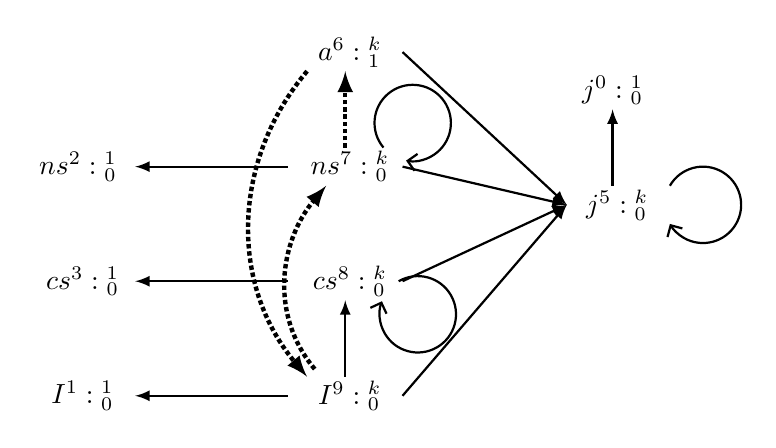
\begin{tikzpicture}[scale=\textwidth/25cm,samples=200]
% Variables Initialization
\draw[] (-7, 1) circle (0pt) node{{ $I^1: {}^1_{0}$}};
\draw[] (-7, 7) circle (0pt) node{{$ns^2: {}^{1}_{0}$}};
\draw[] (-7, 4) circle (0pt) node{{ $cs^3: {}^{1}_{0}$}};
% Variables Inside the Loop
     \draw[] (0, 10) circle (0pt) node{{ $a^6: {}^{k}_{1}$}};
     \draw[] (0, 7) circle (0pt) node{{ $ns^7: {}^{k}_{0}$}};
     \draw[] (0, 4) circle (0pt) node{{ $cs^8: {}^{k}_{0}$}};
     \draw[] (0, 1) circle (0pt) node{{ $I^9: {}^{k}_{0}$}};
     % Counter Variables
     \draw[] (7, 9) circle (0pt) node {{$j^0: {}^{1}_{0}$}};
     \draw[] (7, 6) circle (0pt) node {{ $j^5: {}^{k}_{0}$}};
     %
     % Value Dependency Edges:
     \draw[ thick, -latex,] (0, 1.5)  -- (0, 3.5) ;
     \draw[ ultra thick, -latex, densely dotted,] (0, 7.5)  -- (0, 9.5) ;
     \draw[ thick, -Straight Barb] (1.4, 4) arc (120:-200:1);
     \draw[ thick, -Straight Barb] (8.5, 6.5) arc (150:-150:1);
     \draw[ thick, -Straight Barb] (1, 7.5) arc (220:-100:1);
     \draw[ thick, -latex] (7, 6.5)  -- (7, 8.5) ;
     % Value Dependency Edges on Initial Values:
     \draw[ thick, -latex,] (-1.5, 1)  -- (-5.5, 1) ;
     \draw[ thick, -latex,] (-1.5, 4)  -- (-5.5, 4) ;
     \draw[ thick, -latex,] (-1.5, 7)  -- (-5.5, 7) ;
     %
     \draw[ ultra thick, -latex, densely dotted,] (-1, 9.5)  to  [out=-130,in=130]  (-1, 1.5);
     \draw[ ultra thick, -latex, densely dotted,] (-0.8, 1.7)  to  [out=-230,in=230]  (-0.5, 6.5);
     % Control Dependency
    %  \draw[ thick,-latex] (1.5, 7)  -- (4, 9) ;
    %  \draw[ thick,-latex] (1.5, 4)  -- (4, 9) ;
     \draw[ thick,-latex] (1.5, 7)  -- (5.8, 6) ;
     \draw[ thick,-latex] (1.5, 4)  -- (5.8, 6) ;
     \draw[ thick,-latex] (1.5, 1)  -- (5.8, 6) ;
     \draw[ thick,-latex] (1.5, 10)  -- (5.8, 6) ;
     \end{tikzpicture}
     \caption{}
        \end{centering}
        \end{subfigure}
    \vspace{-0.4cm}
    \caption{(a) The simplified multiple rounds example (b) The program-based dependency graph from $\THESYSTEM$}
    \vspace{-0.5cm}
    \label{fig:multi_graphs}
\end{figure}
%
\end{example}

\input{examples/linearRegressionGD}
\input{examples/multipleRoundsOdd}
\section{Experimental Result}
\label{sec:adapt-eval}
Then I show my implementation of $\THESYSTEM$ and its experimental 
results on $18$ examples including these four examples.
I implemented $\THESYSTEM$ as a tool which takes a labeled command as input  
% labeled command 
and outputs an upper bound on the program adaptivity and on the number of query requests.
This implementation consists of an 
abstract control flow graph generation, weight estimation (as presented in Section~\ref{sec:alg_weightgen}),
edge estimation (as presented in Section~\ref{sec:alg_edgegen}) in Ocaml, 
and the adaptivity computation algorithm shown in Section~\ref{sec:alg_adaptcompute} in Python.
The OCaml program takes the labeled command as input and outputs the program-based dependency graph,
feeds into the python program and the python program provides the adaptivity upper bound and the query number as the final output.

I evaluated this implementation on $17$ example programs with the evaluation results shown  in Table~\ref{tb:imp}.
In this table,
the first column is the name of each program.
For each program $c$, the second column is its intuitive adaptivity rounds,
the third column is the $A(c)$ we defined through our formal semantic model above.
% in Section~\ref{sec:dep_adaptivity}.
In the third column, we use $k$ represent the weight function $w_k$ (in program's execution-based dependency graph) which return value of variable $k$ 
from an initial trace $\trace_0$, same for natural numbers.
The last column is the output of the $\THESYSTEM$ implementation, which consists of two expressions.
The first one is the upper bound for adaptivity and the second one is the 
upper bound for the total number of query requests in the program.

The first 3 programs we evaluated are $ \kw{twoRoundsComplete(k)}$, $ \kw{multipleRoundsComplete(k)}$, 
and the $\kw{linearRegressionGD(k, rate)}$ which we discussed in overview and above section.
% Section~\ref{sec:examples}.
% The same for the third programprograms in the table row 
For these examples, $A(c)$ 
% based dynamic analysis 
give the accurate adaptivity definition, 
simultaneously the $\THESYSTEM$ outputs the tight bounds for both of the adaptivity and query requesting number as expected.
% Look at 
% the $ \kw{linearRegressionGD(k)}$ which we discussed in Section~\ref{sec:examples}, the $\THESYSTEM$ outputs the accurate bound $k$ as expected.
But for the forth program $\kw{multipleRoundOdd(k)}$, $\THESYSTEM$ outputs an over-approximated upper bound $1 + 2*k$ for the $A(c)$, 
which is consistent with our expectation as discussed in Example~\ref{ex:multipleRoundSingle}. 
The fifth program is the evaluation results for the example in Example~\ref{ex:multipleRoundSingle}, where $\THESYSTEM$ outputs
the tight bound for $A(c)$ but $A(c)$ is a loose definition of the program's actual adaptivity rounds.
%
The programs in the table from  $\kw{seq()}$ to $ \kw{nestedWhileMultiPathMultiVarRecAcross(k)}$ are 
designed for testing the programs under different possible situitions.
These programs contain control dependency, data value dependency,
the nested while, dependency through multiple variables, dependency across nested loops, and so on. 
Overall for these examples, our system gives both the accurate adaptivity definition and 
adaptivity upper bound simultaneously through the dynamic analysis and 
static analysis.
The full programs are defined below from Example~\ref{ex:twoRoundsComplete} to Example~\ref{ex:nestedWhileMultiVarRecAcross}.
%
For the other programs, the complete program can be found in Appendix.
\begin {table}[H]
        \vspace{-0.3cm}
    \caption{Experimental results of {\THESYSTEM} implementation}
        \label{tb:imp}
        \begin{center}
        \centering
{\footnotesize
        \begin{tabular}{ r | p{12mm} p{55mm} p{\textwidth}}
         Program $c$ & adaptive \newline rounds & $A(c)$ \newline $w: \mathcal{T}_0(c) \to \mathbb{N}$ & $\THESYSTEM$ \newline $\progA(c)$, $\# \query$ \\ 
         \hline
         $  \kw{twoRoundsComplete(k)}$ & $2$ & $\trace_0 \to 2$ & $2$, $k$ \\
         $  \kw{multipleRoundsComplete(k)}$ & $k$ & $\trace_0 \to \env(\trace_0) k$ & $k$, $k$  \\
         $  \kw{linearRegressionGD(k, rate)}$ & $k$ & $k$ & $k$, $2 * k$  \\
         $  \kw{multipleRoundsOdd(k)}$ & $1 + k$ 
                                    & $
                                        \trace_0 \to 
                                        \left\{\begin{array}{ll}
                                        1 + \env(\trace_0) k & \env(\trace_0) k  \leq 1 \\
                                        1 + 2 * \lceil{(\env(\trace_0) k)} \rceil / 2 & \env(\trace_0) k \geq 2
                                        \end{array}\right\}
                                        $ 
              & $1 + 2*k$, $1 + 2*k$  \\
         $  \kw{multipleRoundsSingle(k)}$    & $2$ 
                                            & $
                                                \trace_0 \to 
                                                \left\{\begin{array}{ll}
                                                \env(\trace_0) k & \env(\trace_0) k  \leq 1 \\
                                                2 & \env(\trace_0) k \geq 2
                                                \end{array}\right\}
                                                $ 
                                            & $2 + k$ , $2 + k$  \\
         $\kw{seq()}$ & $4$ & $4$ & $4$, $4$  \\ 
         $\kw{seqMultiVar()}$ & $4$ & $4$ & $4$, $4$ \\  
         $ \kw{ifValueDependency}$ & $3$ & $3$ & $3$, $3$ \\
         $\kw{ifControlDependency()}$ & $3$ & $3$ & $3$, $3$  \\
         $ \kw{whileRec(k)}$ & $1+k$ & $1+k$ & $1+k$  \\
        %  $ \kw{whileMultiplePath(k)}$ & $1 + k$ & $1 + k$ & $1 + 2 * k$, $1 + 2 * k$  \\
         $ \kw{whileMultipleVar(k)}$ & $1 + 2*k$ & $1 + 2*k$ & $1 + 2*k$, $2 + 3 * k$  \\
         $ \kw{whileValueControlDependency(k)}$ & $1 + 2*k$ & $1 + 2*k$ & $1 + 2 * k$, $2 + 2 * k$  \\
         $ \kw{whileMultiplePathValueControlDependency(k)}$ & $2 + k$ & $2 + k$  & $2 + k$, $1 + 2 * k$   \\
         $ \kw{nestWhileValueDependency(k)}$ & $2 + k^2$ & $2 + k^2$  & $2 + k^2$, $1 + k + k^2$   \\
         $ \kw{nestedWhileRecAcross(k)}$ & $1 + 2*k$ & $1 + 2*k$ & $1 + 2*k$,  $1 + k + k^2$   \\
         $ \kw{nestedWhileMultiVarRecAcross(k)}$ & $1 + k + k^2$ & $1 + k + k^2$  & $1 + k + k^2$,  $2 + k + k^2$  \\
         $ \kw{nestedWhileMultiPathMultiVarRecAcross(k)}$ & $1 + k + k^2$ & $1 + k + k^2$  & $1 + k + k^2$,  $2 + k + k^2$  \\
        \end{tabular}
}        
\end{center}
\end{table}
        %

\begin{example}[Complete Two Round Algorithm]
        \label{ex:twoRoundsComplete}
        \[
        %
            \kw{twoRoundsComplete(k)} \triangleq
        \begin{array}{l}
               \clabel{ a \leftarrow []}^{1} ; \\
                \clabel{\assign{j}{k} }^{2} ; \\
                \ewhile ~ \clabel{j > 0}^{3} ~ \edo ~ \\
                \Big(
                 \clabel{\assign{x}{\query(\chi[k - j]\cdot \chi[k])} }^{4}  ; \\
                 \clabel{\assign{j}{j-1}}^{5} ;\\
                \clabel{a \leftarrow x :: a}^{6}       \Big);\\
                \clabel{l \leftarrow (\kw{sign}\big (\sum_{i\in [k]} \chi[i]\times\ln\frac{1+a[i]}{1-a[i]} \big ))}^{7}\\
            \end{array}
        \]
        %
        \begin{algorithm}
        \footnotesize
        \caption{A two-round analyst strategy for random data (The example in  \cite{dwork2015preserving})}
        \label{alg:twoRound}
        \begin{algorithmic}
        \REQUIRE Mechanism $\mathcal{M}$ with a hidden data set $D \in \{-1,+1\}^{n\times (k+1)} \subset \dbdom$.
        \STATE  {\bf for}\ $j\in [k]$\ {\bf do}.  
        \STATE \qquad {\bf define} $q_j(d)=d(j)\cdot d(k)$ where $d \in \{D(i) ~|~ i = 0, \cdots, n\} \subseteq \{-1,+1\}^{k+1}$.
        \STATE \qquad {\bf let} $a_j=\mathcal{M}(q_j)$ 
        \STATE \qquad \COMMENT{In the line above, $\mathcal{M}$ computes approx. the exp. value  of $q_j$ over $D$. So, $a_j\in [-1,+1]$.}
        \STATE {\bf define} $q_{k}(d)= d(k) \cdot \kw{sign}\big (\sum_{i\in [k]} x(i) \cdot \ln\frac{1+a_i}{1-a_i} \big )$ where $x\in \{-1,+1\}^{k+1}$.
        \STATE\COMMENT{In the line above,  $\kw{sign}(y)=\left \{ \begin{array}{lr} +1 & \kw{if}\ y\geq 0\\ -1 &\kw{otherwise} \end{array} \right . $.}
        \STATE {\bf let} $a_{k+1}=\mathcal{M}(q_{k+1})$
        \STATE\COMMENT{In the line above,  $\mathcal{M}$ computes approx. the exp. value  of $q_{k+1}$ over $X$. So, $a_{k+1}\in [-1,+1]$.}
        \RETURN $a_{k+1}$.
        \ENSURE $a_{k+1}\in [-1,+1]$
            % \ENSURE 
        \end{algorithmic}
        \end{algorithm}
        %
    %
        \end{example}
    
    \begin{example}[Complete Multiple Round Algorithm]
    %
    \begin{algorithm}
    \footnotesize
    \caption{A multi-round analyst strategy for random data base \cite{dwork2015preserving}}
    \label{alg:multiRound}
    \begin{algorithmic}
    \REQUIRE Mechanism $\mathcal{M}$ with a hidden state $X\in [N]^{n}$ sampled u.a.r., control set size $c$
    \STATE Define control dataset $C = \{0,1, \cdots, c - 1\}$
    \STATE Initialize $Nscore(i) = 0$ for $i \in [N]$, $I = \emptyset$ and $Cscore(C(i)) = 0$ for $i \in [c]$
    \STATE  {\bf for}\ $j\in [k]$\ {\bf do} 
    \STATE \qquad {\bf let} $p=\uniform(0,1)$ 
    \STATE \qquad {\bf define} $q (x) = \bernoulli ( p )$ .
    \STATE \qquad {\bf define} $qc (x) = \bernoulli ( p )$ .
    \STATE \qquad {\bf let} $a = \mathcal{M}(q)$ 
    \STATE \qquad {\bf for}\ $i \in [N]$\ {\bf do}
    \STATE \qquad \qquad $Nscore(i) = Nscore(i) + (a - p)*(q (i) - p)$ if $i \notin I$
    \STATE \qquad {\bf for}\ $i \in [c]$\ {\bf do}
    \STATE \qquad \qquad $Cscore(C(i)) = Cscore(C(i)) + (a - p)*(qc (i) - p)$
    \STATE \qquad {\bf let} $I = \{i | i\in [N] \land Nscore(i) > \max(Cscore)\}$
    \STATE \qquad {\bf let} $D = D \setminus I$ 
    \RETURN $D$.
    \end{algorithmic}
    \end{algorithm}
    %
    {\small
    \begin{figure}
        \begin{subfigure}{0.8\textwidth}
        \begin{centering}
        $
    \kw{multipleRoundsComplete(k, c, N)} \triangleq
    \begin{array}{l}
        \clabel{\assign{j}{N}}^0 ; 
         \clabel{\assign{cs}{0}}^1; 
         \clabel{\assign{ns}{0}}^2;
         \clabel{\assign{I}{0}}^3; 
         \clabel{\assign{w}{k}}^{4} ;\\
         \ewhile ~ \clabel{j > 0}^{5} ~ \edo ~ \\
         \Big(
         \clabel{\assign{j}{j-1}}^{6} ;
         \clabel{\assign{cs}{0 + cs}}^7; 
         \clabel{\assign{ns}{0 + ns}}^8
         \Big); \\
    
         \ewhile ~ \clabel{w > 0}^{9} ~ \edo ~ \\
        \Big(
        \clabel{\assign{w}{w-1}}^{10} ;
        \left[p \leftarrow c \right]^{11}; 
        \left[q \leftarrow c \right]^{12}; 
        \left[ a \leftarrow \query (\chi[I]) \right]^{13};\\
        \clabel{\assign{i}{N}}^{14} ; 
        \ewhile ~ \clabel{i > 0}^{15} ~ \edo ~ \\
        \Big(
        \clabel{\assign{i}{i-1}}^{16} ;
        \clabel{\assign{cs(i)}{cs(i) + (a - p) * (q - p)}}^{17}; \\
        \eif (\clabel{ I < i}^{18}, \clabel{\assign{ns(i)}{{ns(i) + (a - p) * (q - p)}}}^{19},
        \clabel{\assign{ns}{ns(i)}}^{20}    )
        \Big); \\
        \clabel{\assign{i2}{N}}^{21} ; \\
        \ewhile ~ \clabel{i2 > 0}^{22} ~ \edo ~ \\
        \Big(
        \clabel{\assign{i2}{i2-1}}^{23} ;
        \eif (\clabel{ns(i2) > \kw{max}(cs)}^{24}, 
        \clabel{\assign{I}{i + I}}^{25},
        \clabel{\assign{I}{I}}^{26})
        \Big)
        \Big) 
    \end{array}
       $
       \caption{}
        \end{centering}
        \end{subfigure}
        \vspace{-0.3cm}
        \caption{(a) The labeled program implementing the multiple round algorithm (b)The same program in the SSA version}
        \vspace{-0.5cm}
        \label{fig:multiround_complete}
        \end{figure}
    }
    %
    \end{example}

\chapter{Related Works\todo{progress-90\% need passes on details}}
\label{sec:adapt-relatedwork}

\section{The Execution-Based Program Analysis}
\label{sec:relatedwork-exe}
My framework constructs an execution-based dependency graph based on the execution traces of a program. 
    I define semantic dependence on this graph by considering (intraprocedural) data and control 
    dependency~\cite{bilardi1996framework,cytron1991efficiently,pollock1989incremental}.    
    One related work  
    \cite{austin1992dynamic} presents a methodology to construct a dynamic dependency graph (DDG) based on the dynamic execution of a program in an imperative language, where edges represent dependency between instructions. Data dependency, control dependency, storage dependency, and resource dependency between instructions are all considered. My execution-based dependency graph only needs data dependency and control dependency between variable assignment results. 
    % Critical path length analysis on DDGs is useful for understanding the scope for parallelization, while we use the length of the longest path to define adaptivity.  
    %
    DDGs have been used in many other domains. \cite{nagar2018automated} use DDGs to find serializability violations. \cite{hammer2006dynamic} use similar \emph{program dependency graphs} \cite{ferrante1987program} for dynamic program slicing.
    \cite{mastroeni2008data} propose ways of constructing different kinds of program slices, by choose different program dependency. 
    % For example, in either syntactic or semantics sense.
    % This abstract dependency is based on properties rather than exact data.
    % Aims to give finer and smaller program slice. 
    They actually use a combination of  
    static and dynamic dependency graphs but in a manner that is different from how we use the two. Their slicing uses both static and dynamic dependency graphs, while we use the dynamic dependency graph as the basis of a definition, which is then soundly approximated by an analysis based on the static dependency graph.-
    
    My execution-based data dependency relation definition over variables 
    is inspired by the method in \cite{Cousot19a}, where the dependency relation is also identified by looking into the differences on two execution traces. 
    However, Cousot excludes timing channels~\cite{SabelfeldM03} and empty observation, which are also not considered as a form of dependency in traditional dependency analysis \cite{DenningD77}.
    % In the cases of empty observation and timing channels, the second query is executed 
    % in one trace and isn't in another trace by modifying value of first query. 
    % Then, the second query is indeed depend on the first query and there exists an
    % adaptivity round between the two queries. 
    My definition includes timing channels and empty observation by observing both the disappearance and value variation.
    % \paragraph*{Analysis Structure}
    % In order to formalize a quantitative property w.r.t. the dependency relation in program, I
    % use a three-step analysis methodology developed, 
    %  as follows,
    % \\
    %  a. The dependency relation between every query, through the methodology of semantic data dependency analysis.
    % \\
    %  b. The dependency quantity analysis, through the methodology of execution-based data reachability bound analysis. Then 
    % \\
    %  c. The adaptivity analysis, based on the two analysis results above, 
    %  I construct an execution-based dependency graph combining the dependency relation and the dependency quantity
    %     and give the formal \emph{adaptivity} definition 
    %     for program.
    %     This analysis is the first part of the analysis in Figure~\ref{fig:structure}.
    


\section{Static Analysis}
\label{sec:relatedwork-static}
\input{chapters/adapt/relatedwork-static}

\section{Generalization in Adaptive Data Analysis}
\label{sec:relatedwork-adapt}
Starting from the works by \citet{DworkFHPRR15} and \citet{HardtU14}, several works have designed methods that ensure generalization for adaptive data analyses.
Some examples
are:~\cite{dwork2015reusable,dwork2015generalization,
BassilyNSSSU16,UllmanSNSS18,FeldmanS17,jung2019new,SteinkeZ20,RogersRSSTW20}.
Several of these works drew inspiration from the idea of using methods designed to ensure differential privacy, a notion of formal data privacy, in order to guarantee generalization for adaptive data analyses.
By limiting the influence that an individual can have on the result of a data analysis, even in adaptive settings, differential privacy can also be used to limit the influence that a specific data sample can have on the statistical validity of a data analysis.
This connection is actually in two directions, as discussed for example by \citet{YeomGFJ18}.

Considering this connection between generalization and privacy, it is not surprising
that some works on programming language techniques for privacy-preserving data analysis are related to our work. 
Adaptive Fuzz~\cite{Winograd-CortHR17} is a programming framework for differential privacy that is designed around the concept of adaptivity. 
This framework is based on a typed functional language that distinguish between several forms of adaptive and non-adaptive composition theorem with the goal of achieving better upper bounds on the privacy cost.
Adaptive Fuzz uses a type system and some partial evaluation to guarantee that the programs respect differential privacy.
However, it does not include any technique to bound the number of rounds of adaptivity. 
\citet{lobo2021programming} propose a language for differential privacy where one can reason about the accuracy of programs in terms of confidence intervals on the error that the use of differential privacy can generate. These are akin to bounds on the generalization error. This language is based on a static analysis which however cannot handle adaptivity. 
%
The way we formalize the access to the data mediated by a mechanism is a reminiscence of how the interaction with an oracle is modeled in the verification of security properties. As an example, the recent works by \citet{BarbosaBGKS21} and \citet{AguirreBGGKS21} use different techniques to track the number of accesses to an oracle. However, reasoning about the number of accesses is easier than estimating the adaptivity of these calls, as we do instead here.


% \cleardoublepage
\chapter*{\redd{PART \romannum{3} \quad Epilogue}}
\chapter*{\redd{ \romannum{4} \quad Epilogue}}

I review the works on studying the quantitative properties in this dissertation in the next part, and the future directions are also discussed. 
% \cleardoublepage
% \chapter*{Future Works}


% \addtocontents{toc}{\protect\newpage}
\chapter{Conclusion\todo{progress-40\% need details for Reachability bounds, emphasis on improvements of Adaptivity Analysis and passes on details}}
\label{sec:conclusion}
\chapter{Conclusion}
\label{ch:conclusion}

In this chapter, we conclude this dissertation, mainly studying two quantitative properties of programs, the relative cost of two programs, and the adaptivity of adaptive data analysis programs. The relative cost can be reasoned about by relational cost analysis, and we will review the work of {\Arel} and its implementation {\BIAREL}. Adaptivity is another topic, the work {\ADAPTSYSTEM} focuses on it.  We
review its key novelties and contributions discuss several directions on the future researches. 


 
 \section{Dynamic}
 
 Another quantitative property is the adaptivity of programs. We presented {\ADAPTSYSTEM}, 
 a program analysis algorithm that is useful to provide an upper bound on the adaptivity of data analysis under a specific data analysis model. 
 This estimation can help data analysts to control the generalization errors of their analyses by choosing different algorithmic techniques based on adaptivity. 
 Besides, a key contribution of our works is the formalization of the notion of adaptivity for adaptive data analysis. 

 There are some limitations of this work. 
 \begin{enumerate}
     \item One limitation is that our algorithm may over-estimate the adaptivity of a program, 
     as shown in Section~\ref{sec:adapt-example-over}, due to its path-insensitive nature when analyzing if conditions. 
     The future direction is to use the constraint to track the necessary information and help to predict the path when the control flow diverges.
     \item Another one is that our algorithm now can only analyze concrete bound for loops. 
     The direction of future work is to support dynamic or unbounded loops. 
 \end{enumerate}
 
 \section{Static}

\clearpage
%
\chapter{Future Works\todo{progress-80\% need simplifies and passes on details}}
\label{sec:future}
\section{Towards Program Non-Monotonic Resource Cost Analysis}
\label{sec:future-cost}
\input{chapters/future-nonmonotonic_cost}

\section{Towards Solving the CFL Reachability Problem}
\label{sec:future-cfl}
\input{chapters/future-cfl_reduction}


\cleardoublepage


%%%%%%%%%%%%%%%%%%%%%%%%%%%%%%%%%%%%%%%%%%%%%%%%%%%%%%%%%%%%%%%%%%
% Quick references for some R packages used that I want in the bibliography
\nocite{tikzDevice,plotly,reshape,Rcomputing,Florida2000}

%%%%%%%%%%%%%%%%%%%%%%%%%%%%%%%%%%%%%%%%%%%%%%%%%%%%%%%%%%%%%%%%%%
% Put your appendices inside here, to maintain figure and table listings. Make sure to use \section{appendixA} to have some numbering for figures and tables.


\addtocontents{toc}{\protect\newpage}
\chapter*{\redd{PART \romannum{4} \quad  Appendix}}
\appendix
% \begin{appendices}
\begingroup
  \hypersetup{linkbordercolor=white,linkcolor=black,
    filecolor=black, urlcolor=black} 
% \addcontentsline{toc}{chapter}{List of Figures in Appendix}
\listofappendixfigures
\endgroup
% \stoplist[main]{lof}% stops main list of figures
% \startlist[appendix]{lof}
% \printlist[appendix]{lof}{}{\chapter*{List of Figures in Appendix}}
% % \include{chapters/Glossary}
% \addtocontents{toc}{\protect\newpage}
% \chapter*{\redd{PART \romannum{1} \quad  REACHABILITY BOUND ANALYSIS}}
%
\chapter{Appendix for REACHABILITY BOUND ANALYSIS}
\label{apdx:reachability}
\section{Complete Examples Evaluted in Implementation}
\label{appendix:implementation}
Then I show my implementation of $\THESYSTEM$ and its experimental 
results on $18$ examples including these four examples.
I implemented $\THESYSTEM$ as a tool which takes a labeled command as input  
% labeled command 
and outputs an upper bound on the program adaptivity and on the number of query requests.
This implementation consists of an 
abstract control flow graph generation, weight estimation (as presented in Section~\ref{sec:alg_weightgen}),
edge estimation (as presented in Section~\ref{sec:alg_edgegen}) in Ocaml, 
and the adaptivity computation algorithm shown in Section~\ref{sec:alg_adaptcompute} in Python.
The OCaml program takes the labeled command as input and outputs the program-based dependency graph,
feeds into the python program and the python program provides the adaptivity upper bound and the query number as the final output.

I evaluated this implementation on $17$ example programs with the evaluation results shown  in Table~\ref{tb:imp}.
In this table,
the first column is the name of each program.
For each program $c$, the second column is its intuitive adaptivity rounds,
the third column is the $A(c)$ we defined through our formal semantic model above.
% in Section~\ref{sec:dep_adaptivity}.
In the third column, we use $k$ represent the weight function $w_k$ (in program's execution-based dependency graph) which return value of variable $k$ 
from an initial trace $\trace_0$, same for natural numbers.
The last column is the output of the $\THESYSTEM$ implementation, which consists of two expressions.
The first one is the upper bound for adaptivity and the second one is the 
upper bound for the total number of query requests in the program.

The first 3 programs we evaluated are $ \kw{twoRoundsComplete(k)}$, $ \kw{multipleRoundsComplete(k)}$, 
and the $\kw{linearRegressionGD(k, rate)}$ which we discussed in overview and above section.
% Section~\ref{sec:examples}.
% The same for the third programprograms in the table row 
For these examples, $A(c)$ 
% based dynamic analysis 
give the accurate adaptivity definition, 
simultaneously the $\THESYSTEM$ outputs the tight bounds for both of the adaptivity and query requesting number as expected.
% Look at 
% the $ \kw{linearRegressionGD(k)}$ which we discussed in Section~\ref{sec:examples}, the $\THESYSTEM$ outputs the accurate bound $k$ as expected.
But for the forth program $\kw{multipleRoundOdd(k)}$, $\THESYSTEM$ outputs an over-approximated upper bound $1 + 2*k$ for the $A(c)$, 
which is consistent with our expectation as discussed in Example~\ref{ex:multipleRoundSingle}. 
The fifth program is the evaluation results for the example in Example~\ref{ex:multipleRoundSingle}, where $\THESYSTEM$ outputs
the tight bound for $A(c)$ but $A(c)$ is a loose definition of the program's actual adaptivity rounds.
%
The programs in the table from  $\kw{seq()}$ to $ \kw{nestedWhileMultiPathMultiVarRecAcross(k)}$ are 
designed for testing the programs under different possible situitions.
These programs contain control dependency, data value dependency,
the nested while, dependency through multiple variables, dependency across nested loops, and so on. 
Overall for these examples, our system gives both the accurate adaptivity definition and 
adaptivity upper bound simultaneously through the dynamic analysis and 
static analysis.
The full programs are defined below from Example~\ref{ex:twoRoundsComplete} to Example~\ref{ex:nestedWhileMultiVarRecAcross}.
%
For the other programs, the complete program can be found in Appendix.
\begin {table}[H]
        \vspace{-0.3cm}
    \caption{Experimental results of {\THESYSTEM} implementation}
        \label{tb:imp}
        \begin{center}
        \centering
{\footnotesize
        \begin{tabular}{ r | p{12mm} p{55mm} p{\textwidth}}
         Program $c$ & adaptive \newline rounds & $A(c)$ \newline $w: \mathcal{T}_0(c) \to \mathbb{N}$ & $\THESYSTEM$ \newline $\progA(c)$, $\# \query$ \\ 
         \hline
         $  \kw{twoRoundsComplete(k)}$ & $2$ & $\trace_0 \to 2$ & $2$, $k$ \\
         $  \kw{multipleRoundsComplete(k)}$ & $k$ & $\trace_0 \to \env(\trace_0) k$ & $k$, $k$  \\
         $  \kw{linearRegressionGD(k, rate)}$ & $k$ & $k$ & $k$, $2 * k$  \\
         $  \kw{multipleRoundsOdd(k)}$ & $1 + k$ 
                                    & $
                                        \trace_0 \to 
                                        \left\{\begin{array}{ll}
                                        1 + \env(\trace_0) k & \env(\trace_0) k  \leq 1 \\
                                        1 + 2 * \lceil{(\env(\trace_0) k)} \rceil / 2 & \env(\trace_0) k \geq 2
                                        \end{array}\right\}
                                        $ 
              & $1 + 2*k$, $1 + 2*k$  \\
         $  \kw{multipleRoundsSingle(k)}$    & $2$ 
                                            & $
                                                \trace_0 \to 
                                                \left\{\begin{array}{ll}
                                                \env(\trace_0) k & \env(\trace_0) k  \leq 1 \\
                                                2 & \env(\trace_0) k \geq 2
                                                \end{array}\right\}
                                                $ 
                                            & $2 + k$ , $2 + k$  \\
         $\kw{seq()}$ & $4$ & $4$ & $4$, $4$  \\ 
         $\kw{seqMultiVar()}$ & $4$ & $4$ & $4$, $4$ \\  
         $ \kw{ifValueDependency}$ & $3$ & $3$ & $3$, $3$ \\
         $\kw{ifControlDependency()}$ & $3$ & $3$ & $3$, $3$  \\
         $ \kw{whileRec(k)}$ & $1+k$ & $1+k$ & $1+k$  \\
        %  $ \kw{whileMultiplePath(k)}$ & $1 + k$ & $1 + k$ & $1 + 2 * k$, $1 + 2 * k$  \\
         $ \kw{whileMultipleVar(k)}$ & $1 + 2*k$ & $1 + 2*k$ & $1 + 2*k$, $2 + 3 * k$  \\
         $ \kw{whileValueControlDependency(k)}$ & $1 + 2*k$ & $1 + 2*k$ & $1 + 2 * k$, $2 + 2 * k$  \\
         $ \kw{whileMultiplePathValueControlDependency(k)}$ & $2 + k$ & $2 + k$  & $2 + k$, $1 + 2 * k$   \\
         $ \kw{nestWhileValueDependency(k)}$ & $2 + k^2$ & $2 + k^2$  & $2 + k^2$, $1 + k + k^2$   \\
         $ \kw{nestedWhileRecAcross(k)}$ & $1 + 2*k$ & $1 + 2*k$ & $1 + 2*k$,  $1 + k + k^2$   \\
         $ \kw{nestedWhileMultiVarRecAcross(k)}$ & $1 + k + k^2$ & $1 + k + k^2$  & $1 + k + k^2$,  $2 + k + k^2$  \\
         $ \kw{nestedWhileMultiPathMultiVarRecAcross(k)}$ & $1 + k + k^2$ & $1 + k + k^2$  & $1 + k + k^2$,  $2 + k + k^2$  \\
        \end{tabular}
}        
\end{center}
\end{table}
        %

\begin{example}[Complete Two Round Algorithm]
        \label{ex:twoRoundsComplete}
        \[
        %
            \kw{twoRoundsComplete(k)} \triangleq
        \begin{array}{l}
               \clabel{ a \leftarrow []}^{1} ; \\
                \clabel{\assign{j}{k} }^{2} ; \\
                \ewhile ~ \clabel{j > 0}^{3} ~ \edo ~ \\
                \Big(
                 \clabel{\assign{x}{\query(\chi[k - j]\cdot \chi[k])} }^{4}  ; \\
                 \clabel{\assign{j}{j-1}}^{5} ;\\
                \clabel{a \leftarrow x :: a}^{6}       \Big);\\
                \clabel{l \leftarrow (\kw{sign}\big (\sum_{i\in [k]} \chi[i]\times\ln\frac{1+a[i]}{1-a[i]} \big ))}^{7}\\
            \end{array}
        \]
        %
        \begin{algorithm}
        \footnotesize
        \caption{A two-round analyst strategy for random data (The example in  \cite{dwork2015preserving})}
        \label{alg:twoRound}
        \begin{algorithmic}
        \REQUIRE Mechanism $\mathcal{M}$ with a hidden data set $D \in \{-1,+1\}^{n\times (k+1)} \subset \dbdom$.
        \STATE  {\bf for}\ $j\in [k]$\ {\bf do}.  
        \STATE \qquad {\bf define} $q_j(d)=d(j)\cdot d(k)$ where $d \in \{D(i) ~|~ i = 0, \cdots, n\} \subseteq \{-1,+1\}^{k+1}$.
        \STATE \qquad {\bf let} $a_j=\mathcal{M}(q_j)$ 
        \STATE \qquad \COMMENT{In the line above, $\mathcal{M}$ computes approx. the exp. value  of $q_j$ over $D$. So, $a_j\in [-1,+1]$.}
        \STATE {\bf define} $q_{k}(d)= d(k) \cdot \kw{sign}\big (\sum_{i\in [k]} x(i) \cdot \ln\frac{1+a_i}{1-a_i} \big )$ where $x\in \{-1,+1\}^{k+1}$.
        \STATE\COMMENT{In the line above,  $\kw{sign}(y)=\left \{ \begin{array}{lr} +1 & \kw{if}\ y\geq 0\\ -1 &\kw{otherwise} \end{array} \right . $.}
        \STATE {\bf let} $a_{k+1}=\mathcal{M}(q_{k+1})$
        \STATE\COMMENT{In the line above,  $\mathcal{M}$ computes approx. the exp. value  of $q_{k+1}$ over $X$. So, $a_{k+1}\in [-1,+1]$.}
        \RETURN $a_{k+1}$.
        \ENSURE $a_{k+1}\in [-1,+1]$
            % \ENSURE 
        \end{algorithmic}
        \end{algorithm}
        %
    %
        \end{example}
    
    \begin{example}[Complete Multiple Round Algorithm]
    %
    \begin{algorithm}
    \footnotesize
    \caption{A multi-round analyst strategy for random data base \cite{dwork2015preserving}}
    \label{alg:multiRound}
    \begin{algorithmic}
    \REQUIRE Mechanism $\mathcal{M}$ with a hidden state $X\in [N]^{n}$ sampled u.a.r., control set size $c$
    \STATE Define control dataset $C = \{0,1, \cdots, c - 1\}$
    \STATE Initialize $Nscore(i) = 0$ for $i \in [N]$, $I = \emptyset$ and $Cscore(C(i)) = 0$ for $i \in [c]$
    \STATE  {\bf for}\ $j\in [k]$\ {\bf do} 
    \STATE \qquad {\bf let} $p=\uniform(0,1)$ 
    \STATE \qquad {\bf define} $q (x) = \bernoulli ( p )$ .
    \STATE \qquad {\bf define} $qc (x) = \bernoulli ( p )$ .
    \STATE \qquad {\bf let} $a = \mathcal{M}(q)$ 
    \STATE \qquad {\bf for}\ $i \in [N]$\ {\bf do}
    \STATE \qquad \qquad $Nscore(i) = Nscore(i) + (a - p)*(q (i) - p)$ if $i \notin I$
    \STATE \qquad {\bf for}\ $i \in [c]$\ {\bf do}
    \STATE \qquad \qquad $Cscore(C(i)) = Cscore(C(i)) + (a - p)*(qc (i) - p)$
    \STATE \qquad {\bf let} $I = \{i | i\in [N] \land Nscore(i) > \max(Cscore)\}$
    \STATE \qquad {\bf let} $D = D \setminus I$ 
    \RETURN $D$.
    \end{algorithmic}
    \end{algorithm}
    %
    {\small
    \begin{figure}
        \begin{subfigure}{0.8\textwidth}
        \begin{centering}
        $
    \kw{multipleRoundsComplete(k, c, N)} \triangleq
    \begin{array}{l}
        \clabel{\assign{j}{N}}^0 ; 
         \clabel{\assign{cs}{0}}^1; 
         \clabel{\assign{ns}{0}}^2;
         \clabel{\assign{I}{0}}^3; 
         \clabel{\assign{w}{k}}^{4} ;\\
         \ewhile ~ \clabel{j > 0}^{5} ~ \edo ~ \\
         \Big(
         \clabel{\assign{j}{j-1}}^{6} ;
         \clabel{\assign{cs}{0 + cs}}^7; 
         \clabel{\assign{ns}{0 + ns}}^8
         \Big); \\
    
         \ewhile ~ \clabel{w > 0}^{9} ~ \edo ~ \\
        \Big(
        \clabel{\assign{w}{w-1}}^{10} ;
        \left[p \leftarrow c \right]^{11}; 
        \left[q \leftarrow c \right]^{12}; 
        \left[ a \leftarrow \query (\chi[I]) \right]^{13};\\
        \clabel{\assign{i}{N}}^{14} ; 
        \ewhile ~ \clabel{i > 0}^{15} ~ \edo ~ \\
        \Big(
        \clabel{\assign{i}{i-1}}^{16} ;
        \clabel{\assign{cs(i)}{cs(i) + (a - p) * (q - p)}}^{17}; \\
        \eif (\clabel{ I < i}^{18}, \clabel{\assign{ns(i)}{{ns(i) + (a - p) * (q - p)}}}^{19},
        \clabel{\assign{ns}{ns(i)}}^{20}    )
        \Big); \\
        \clabel{\assign{i2}{N}}^{21} ; \\
        \ewhile ~ \clabel{i2 > 0}^{22} ~ \edo ~ \\
        \Big(
        \clabel{\assign{i2}{i2-1}}^{23} ;
        \eif (\clabel{ns(i2) > \kw{max}(cs)}^{24}, 
        \clabel{\assign{I}{i + I}}^{25},
        \clabel{\assign{I}{I}}^{26})
        \Big)
        \Big) 
    \end{array}
       $
       \caption{}
        \end{centering}
        \end{subfigure}
        \vspace{-0.3cm}
        \caption{(a) The labeled program implementing the multiple round algorithm (b)The same program in the SSA version}
        \vspace{-0.5cm}
        \label{fig:multiround_complete}
        \end{figure}
    }
    %
    \end{example}

\section{Theorems and Proofs}
%  in Section~\ref{sec:adapt-language},~\refeq{sec:adapt-exe},~\refeq{sec:adapt-static}}
\label{appendix:thm-adaptivity}
\subsection{Lemmas in Section~\ref{sec:adapt-language}}
\label{apdx:lemma_sec123}
\input{chapters/appendices/thm-adaptivity/lem_section123}
\clearpage
\subsection{Soundness of The New Adaptivity Analysis Framework in Section~\ref{sec:adapt-analysis}}
\label{apdx:adapt_soundness}
\input{chapters/appendices/thm-adaptivity/adapt_soundness}
\input{chapters/appendices/thm-adaptivity/lem_adaptgraph}
\clearpage
% \subsection{Soundness of Accurate Full-Spectrum Adaptivity Analysis}
% \label{apdx:adapt_soundness_extend}

%%%%%%%%%%%%%%%%%%%%%%%%%%%%%%%%% The extra proofs for improved version.%%%%%%%%%%%%%%%%%%%%%%%%%%%%%%%%%%%%%%%%%%%%%%%%%%%%%%%%%%%%%%%%%%
\input{chapters/appendices/thm-improved/adapt_soundness_extend}
\input{chapters/appendices/thm-improved/lem_adaptgraph_extend}
\clearpage
%%%%%%%%%%%%%%%%%%%%%%%%%%%%%%%%%%%%%%%%%%%%%%%%%%%%%%%%%%%%%%%%%%%%%%%%%%%%%%%%%%%%%%%%%%%%%%%%%%%%%%%%%%%%%%%%%%%%%%%%%%%%%%%%%%%%

\subsection{Soundness of $\THESYSTEM$'s Data Dependency Analysis w.r.t. Event Dependency}
\subsubsection{Proof of the Soundness of $\flowsto$}
\label{apdx:flowsto_soundness}
\input{chapters/appendices/thm-adaptivity/flowsto_soundness}
\clearpage
\subsubsection{Proof of the Soundness of $\flowsto$ w.r.t. the Event}
\label{apdx:flowsto_event_soundness}
\input{chapters/appendices/thm-adaptivity/flowsto_event_soundness}
\input{chapters/appendices/thm-adaptivity/lem_depinversion}
\clearpage
%%%%%%%%%%%%%%%%%%%%%%%%%%%%%%%%% The extra proofs for improved version.%%%%%%%%%%%%%%%%%%%%%%%%%%%%%%%%%%%%%%%%%%%%%%%%%%%%%%%%%%%%%%%%%%
\subsection{Soundness of {\THESYSTEM}'s Data Dependency Analysis w.r.t. Two Witness Traces}
\label{apdx:flowsto_soundness_extend}
\input{chapters/appendices/thm-improved/flowsto_soundness_extend}
\paragraph*{Arithmetic Inversions}
The Inversion Lemmas on expression evaluations is in Appendix~\ref{apdx:flowsto_event_soundness}
\paragraph*{Events and Dependency Inversions}
The Inversion Lemmas on \emph{may-dependency} relation, trace and event.
\input{chapters/appendices/thm-improved/lem_depinversion_extend}
%%%%%%%%%%%%%%%%%%%%%%%%%%%%%%%%%%%%%%%%%%%%%%%%%%%%%%%%%%%%%%%%%%%%%%%%%%%%%%%%%%%%%%%%%%%%%%%%%%%%%%%%%%%%%%%%%%%%%%%%%%%%%%%%%%%%

\subsection{Soundness of $\THESYSTEM$'s Data Dependency Quantity Analysis}
\label{apdx:reachability_soundness}
\input{chapters/appendices/thm-adaptivity/reachability_soundness}
%%%%%%%%%%%%%%%%%%%%%%%%%%%%%%%%%The extra proofs for improved version.%%%%%%%%%%%%%%%%%%%%%%%%%%%%%%%%%%%%%%%%%%%%%%%%%%%%%%%%%%%%%%%%%%
\input{chapters/appendices/thm-improved/ps_reachability_soundness}
\input{chapters/appendices/thm-improved/edgeweight_soundness}
%%%%%%%%%%%%%%%%%%%%%%%%%%%%%%%%%%%%%%%%%%%%%%%%%%%%%%%%%%%%%%%%%%%%%%%%%%%%%%%%%%%%%%%%%%%%%%%%%%%%%%%%%%%%%%%%%%%%%%%%%%%%%%%%%%%%
\clearpage
\subsection{Soundness of Adaptivity Computation Algorithm}
\label{apdx:adaptalg_soundness}
\input{chapters/appendices/thm-adaptivity/adaptalg_soundness}
% %
\subsection{Conditional Completeness of Adaptivity Computation Algorithm}
\label{apdx:adaptalg_completeness}
\input{chapters/appendices/thm-adaptivity/adaptalg_completeness}
\clearpage

% \section{Theorems and Proofs in Section~\ref{ch:improved}}
% \label{appendix:thm-improved}
% \subsection{Soundness of Accurate Full-Spectrum Adaptivity Analysis}
% \label{apdx:adapt_soundness_extend}
% \input{chapters/appendices/thm-improved/adapt_soundness_extend}
% \input{chapters/appendices/thm-improved/lem_adaptgraph_extend}
% \clearpage

% \subsection{Soundness of Improved $\THESYSTEM$'s Data Dependency Analysis}
% \label{apdx:flowsto_soundness_extend}
% \input{chapters/appendices/thm-improved/flowsto_soundness_extend}
% \paragraph*{Arithmetic Inversions}
% The Inversion Lemmas on expression evaluations is in Appendix~\ref{apdx:flowsto_event_soundness}
% \paragraph*{Events and Dependency Inversions}
% The Inversion Lemmas on \emph{may-dependency} relation, trace and event.
% \input{chapters/appendices/thm-improved/lem_depinversion_extend}
% \clearpage

% \subsection{Soundness of Path Sensitive Reachability Bounds Estimation}
% \label{apdx:ps_reachability_soundness}
% \input{chapters/appendices/thm-improved/ps_reachability_soundness}
% \clearpage
% \subsection{Soundness of Improved $\THESYSTEM$'s Data Dependency Quantity Analysis}
% \label{apdx:edgeweight_soundness}
% \input{chapters/appendices/thm-improved/edgeweight_soundness}
% \clearpage

% \section{Theorems and Proofs in Section~\ref{ch:generalization}}
% \label{appendix:thm-generalization}
% \input{chapters/appendices/theorems}
\clearpage

% \chapter*{\redd{PART \romannum{2} \quad  PROGRAM ANALYSIS FRAMEWORK FOR ADAPTIVE DATA ANALYSIS}}
\chapter{Appendix for PROGRAM ANALYSIS FRAMEWORK FOR ADAPTIVE DATA ANALYSIS}
\label{apdx:adapt}
\section{Complete Examples Evaluted in Implementation}
\label{appendix:implementation}
Then I show my implementation of $\THESYSTEM$ and its experimental 
results on $18$ examples including these four examples.
I implemented $\THESYSTEM$ as a tool which takes a labeled command as input  
% labeled command 
and outputs an upper bound on the program adaptivity and on the number of query requests.
This implementation consists of an 
abstract control flow graph generation, weight estimation (as presented in Section~\ref{sec:alg_weightgen}),
edge estimation (as presented in Section~\ref{sec:alg_edgegen}) in Ocaml, 
and the adaptivity computation algorithm shown in Section~\ref{sec:alg_adaptcompute} in Python.
The OCaml program takes the labeled command as input and outputs the program-based dependency graph,
feeds into the python program and the python program provides the adaptivity upper bound and the query number as the final output.

I evaluated this implementation on $17$ example programs with the evaluation results shown  in Table~\ref{tb:imp}.
In this table,
the first column is the name of each program.
For each program $c$, the second column is its intuitive adaptivity rounds,
the third column is the $A(c)$ we defined through our formal semantic model above.
% in Section~\ref{sec:dep_adaptivity}.
In the third column, we use $k$ represent the weight function $w_k$ (in program's execution-based dependency graph) which return value of variable $k$ 
from an initial trace $\trace_0$, same for natural numbers.
The last column is the output of the $\THESYSTEM$ implementation, which consists of two expressions.
The first one is the upper bound for adaptivity and the second one is the 
upper bound for the total number of query requests in the program.

The first 3 programs we evaluated are $ \kw{twoRoundsComplete(k)}$, $ \kw{multipleRoundsComplete(k)}$, 
and the $\kw{linearRegressionGD(k, rate)}$ which we discussed in overview and above section.
% Section~\ref{sec:examples}.
% The same for the third programprograms in the table row 
For these examples, $A(c)$ 
% based dynamic analysis 
give the accurate adaptivity definition, 
simultaneously the $\THESYSTEM$ outputs the tight bounds for both of the adaptivity and query requesting number as expected.
% Look at 
% the $ \kw{linearRegressionGD(k)}$ which we discussed in Section~\ref{sec:examples}, the $\THESYSTEM$ outputs the accurate bound $k$ as expected.
But for the forth program $\kw{multipleRoundOdd(k)}$, $\THESYSTEM$ outputs an over-approximated upper bound $1 + 2*k$ for the $A(c)$, 
which is consistent with our expectation as discussed in Example~\ref{ex:multipleRoundSingle}. 
The fifth program is the evaluation results for the example in Example~\ref{ex:multipleRoundSingle}, where $\THESYSTEM$ outputs
the tight bound for $A(c)$ but $A(c)$ is a loose definition of the program's actual adaptivity rounds.
%
The programs in the table from  $\kw{seq()}$ to $ \kw{nestedWhileMultiPathMultiVarRecAcross(k)}$ are 
designed for testing the programs under different possible situitions.
These programs contain control dependency, data value dependency,
the nested while, dependency through multiple variables, dependency across nested loops, and so on. 
Overall for these examples, our system gives both the accurate adaptivity definition and 
adaptivity upper bound simultaneously through the dynamic analysis and 
static analysis.
The full programs are defined below from Example~\ref{ex:twoRoundsComplete} to Example~\ref{ex:nestedWhileMultiVarRecAcross}.
%
For the other programs, the complete program can be found in Appendix.
\begin {table}[H]
        \vspace{-0.3cm}
    \caption{Experimental results of {\THESYSTEM} implementation}
        \label{tb:imp}
        \begin{center}
        \centering
{\footnotesize
        \begin{tabular}{ r | p{12mm} p{55mm} p{\textwidth}}
         Program $c$ & adaptive \newline rounds & $A(c)$ \newline $w: \mathcal{T}_0(c) \to \mathbb{N}$ & $\THESYSTEM$ \newline $\progA(c)$, $\# \query$ \\ 
         \hline
         $  \kw{twoRoundsComplete(k)}$ & $2$ & $\trace_0 \to 2$ & $2$, $k$ \\
         $  \kw{multipleRoundsComplete(k)}$ & $k$ & $\trace_0 \to \env(\trace_0) k$ & $k$, $k$  \\
         $  \kw{linearRegressionGD(k, rate)}$ & $k$ & $k$ & $k$, $2 * k$  \\
         $  \kw{multipleRoundsOdd(k)}$ & $1 + k$ 
                                    & $
                                        \trace_0 \to 
                                        \left\{\begin{array}{ll}
                                        1 + \env(\trace_0) k & \env(\trace_0) k  \leq 1 \\
                                        1 + 2 * \lceil{(\env(\trace_0) k)} \rceil / 2 & \env(\trace_0) k \geq 2
                                        \end{array}\right\}
                                        $ 
              & $1 + 2*k$, $1 + 2*k$  \\
         $  \kw{multipleRoundsSingle(k)}$    & $2$ 
                                            & $
                                                \trace_0 \to 
                                                \left\{\begin{array}{ll}
                                                \env(\trace_0) k & \env(\trace_0) k  \leq 1 \\
                                                2 & \env(\trace_0) k \geq 2
                                                \end{array}\right\}
                                                $ 
                                            & $2 + k$ , $2 + k$  \\
         $\kw{seq()}$ & $4$ & $4$ & $4$, $4$  \\ 
         $\kw{seqMultiVar()}$ & $4$ & $4$ & $4$, $4$ \\  
         $ \kw{ifValueDependency}$ & $3$ & $3$ & $3$, $3$ \\
         $\kw{ifControlDependency()}$ & $3$ & $3$ & $3$, $3$  \\
         $ \kw{whileRec(k)}$ & $1+k$ & $1+k$ & $1+k$  \\
        %  $ \kw{whileMultiplePath(k)}$ & $1 + k$ & $1 + k$ & $1 + 2 * k$, $1 + 2 * k$  \\
         $ \kw{whileMultipleVar(k)}$ & $1 + 2*k$ & $1 + 2*k$ & $1 + 2*k$, $2 + 3 * k$  \\
         $ \kw{whileValueControlDependency(k)}$ & $1 + 2*k$ & $1 + 2*k$ & $1 + 2 * k$, $2 + 2 * k$  \\
         $ \kw{whileMultiplePathValueControlDependency(k)}$ & $2 + k$ & $2 + k$  & $2 + k$, $1 + 2 * k$   \\
         $ \kw{nestWhileValueDependency(k)}$ & $2 + k^2$ & $2 + k^2$  & $2 + k^2$, $1 + k + k^2$   \\
         $ \kw{nestedWhileRecAcross(k)}$ & $1 + 2*k$ & $1 + 2*k$ & $1 + 2*k$,  $1 + k + k^2$   \\
         $ \kw{nestedWhileMultiVarRecAcross(k)}$ & $1 + k + k^2$ & $1 + k + k^2$  & $1 + k + k^2$,  $2 + k + k^2$  \\
         $ \kw{nestedWhileMultiPathMultiVarRecAcross(k)}$ & $1 + k + k^2$ & $1 + k + k^2$  & $1 + k + k^2$,  $2 + k + k^2$  \\
        \end{tabular}
}        
\end{center}
\end{table}
        %

\begin{example}[Complete Two Round Algorithm]
        \label{ex:twoRoundsComplete}
        \[
        %
            \kw{twoRoundsComplete(k)} \triangleq
        \begin{array}{l}
               \clabel{ a \leftarrow []}^{1} ; \\
                \clabel{\assign{j}{k} }^{2} ; \\
                \ewhile ~ \clabel{j > 0}^{3} ~ \edo ~ \\
                \Big(
                 \clabel{\assign{x}{\query(\chi[k - j]\cdot \chi[k])} }^{4}  ; \\
                 \clabel{\assign{j}{j-1}}^{5} ;\\
                \clabel{a \leftarrow x :: a}^{6}       \Big);\\
                \clabel{l \leftarrow (\kw{sign}\big (\sum_{i\in [k]} \chi[i]\times\ln\frac{1+a[i]}{1-a[i]} \big ))}^{7}\\
            \end{array}
        \]
        %
        \begin{algorithm}
        \footnotesize
        \caption{A two-round analyst strategy for random data (The example in  \cite{dwork2015preserving})}
        \label{alg:twoRound}
        \begin{algorithmic}
        \REQUIRE Mechanism $\mathcal{M}$ with a hidden data set $D \in \{-1,+1\}^{n\times (k+1)} \subset \dbdom$.
        \STATE  {\bf for}\ $j\in [k]$\ {\bf do}.  
        \STATE \qquad {\bf define} $q_j(d)=d(j)\cdot d(k)$ where $d \in \{D(i) ~|~ i = 0, \cdots, n\} \subseteq \{-1,+1\}^{k+1}$.
        \STATE \qquad {\bf let} $a_j=\mathcal{M}(q_j)$ 
        \STATE \qquad \COMMENT{In the line above, $\mathcal{M}$ computes approx. the exp. value  of $q_j$ over $D$. So, $a_j\in [-1,+1]$.}
        \STATE {\bf define} $q_{k}(d)= d(k) \cdot \kw{sign}\big (\sum_{i\in [k]} x(i) \cdot \ln\frac{1+a_i}{1-a_i} \big )$ where $x\in \{-1,+1\}^{k+1}$.
        \STATE\COMMENT{In the line above,  $\kw{sign}(y)=\left \{ \begin{array}{lr} +1 & \kw{if}\ y\geq 0\\ -1 &\kw{otherwise} \end{array} \right . $.}
        \STATE {\bf let} $a_{k+1}=\mathcal{M}(q_{k+1})$
        \STATE\COMMENT{In the line above,  $\mathcal{M}$ computes approx. the exp. value  of $q_{k+1}$ over $X$. So, $a_{k+1}\in [-1,+1]$.}
        \RETURN $a_{k+1}$.
        \ENSURE $a_{k+1}\in [-1,+1]$
            % \ENSURE 
        \end{algorithmic}
        \end{algorithm}
        %
    %
        \end{example}
    
    \begin{example}[Complete Multiple Round Algorithm]
    %
    \begin{algorithm}
    \footnotesize
    \caption{A multi-round analyst strategy for random data base \cite{dwork2015preserving}}
    \label{alg:multiRound}
    \begin{algorithmic}
    \REQUIRE Mechanism $\mathcal{M}$ with a hidden state $X\in [N]^{n}$ sampled u.a.r., control set size $c$
    \STATE Define control dataset $C = \{0,1, \cdots, c - 1\}$
    \STATE Initialize $Nscore(i) = 0$ for $i \in [N]$, $I = \emptyset$ and $Cscore(C(i)) = 0$ for $i \in [c]$
    \STATE  {\bf for}\ $j\in [k]$\ {\bf do} 
    \STATE \qquad {\bf let} $p=\uniform(0,1)$ 
    \STATE \qquad {\bf define} $q (x) = \bernoulli ( p )$ .
    \STATE \qquad {\bf define} $qc (x) = \bernoulli ( p )$ .
    \STATE \qquad {\bf let} $a = \mathcal{M}(q)$ 
    \STATE \qquad {\bf for}\ $i \in [N]$\ {\bf do}
    \STATE \qquad \qquad $Nscore(i) = Nscore(i) + (a - p)*(q (i) - p)$ if $i \notin I$
    \STATE \qquad {\bf for}\ $i \in [c]$\ {\bf do}
    \STATE \qquad \qquad $Cscore(C(i)) = Cscore(C(i)) + (a - p)*(qc (i) - p)$
    \STATE \qquad {\bf let} $I = \{i | i\in [N] \land Nscore(i) > \max(Cscore)\}$
    \STATE \qquad {\bf let} $D = D \setminus I$ 
    \RETURN $D$.
    \end{algorithmic}
    \end{algorithm}
    %
    {\small
    \begin{figure}
        \begin{subfigure}{0.8\textwidth}
        \begin{centering}
        $
    \kw{multipleRoundsComplete(k, c, N)} \triangleq
    \begin{array}{l}
        \clabel{\assign{j}{N}}^0 ; 
         \clabel{\assign{cs}{0}}^1; 
         \clabel{\assign{ns}{0}}^2;
         \clabel{\assign{I}{0}}^3; 
         \clabel{\assign{w}{k}}^{4} ;\\
         \ewhile ~ \clabel{j > 0}^{5} ~ \edo ~ \\
         \Big(
         \clabel{\assign{j}{j-1}}^{6} ;
         \clabel{\assign{cs}{0 + cs}}^7; 
         \clabel{\assign{ns}{0 + ns}}^8
         \Big); \\
    
         \ewhile ~ \clabel{w > 0}^{9} ~ \edo ~ \\
        \Big(
        \clabel{\assign{w}{w-1}}^{10} ;
        \left[p \leftarrow c \right]^{11}; 
        \left[q \leftarrow c \right]^{12}; 
        \left[ a \leftarrow \query (\chi[I]) \right]^{13};\\
        \clabel{\assign{i}{N}}^{14} ; 
        \ewhile ~ \clabel{i > 0}^{15} ~ \edo ~ \\
        \Big(
        \clabel{\assign{i}{i-1}}^{16} ;
        \clabel{\assign{cs(i)}{cs(i) + (a - p) * (q - p)}}^{17}; \\
        \eif (\clabel{ I < i}^{18}, \clabel{\assign{ns(i)}{{ns(i) + (a - p) * (q - p)}}}^{19},
        \clabel{\assign{ns}{ns(i)}}^{20}    )
        \Big); \\
        \clabel{\assign{i2}{N}}^{21} ; \\
        \ewhile ~ \clabel{i2 > 0}^{22} ~ \edo ~ \\
        \Big(
        \clabel{\assign{i2}{i2-1}}^{23} ;
        \eif (\clabel{ns(i2) > \kw{max}(cs)}^{24}, 
        \clabel{\assign{I}{i + I}}^{25},
        \clabel{\assign{I}{I}}^{26})
        \Big)
        \Big) 
    \end{array}
       $
       \caption{}
        \end{centering}
        \end{subfigure}
        \vspace{-0.3cm}
        \caption{(a) The labeled program implementing the multiple round algorithm (b)The same program in the SSA version}
        \vspace{-0.5cm}
        \label{fig:multiround_complete}
        \end{figure}
    }
    %
    \end{example}

\section{Theorems and Proofs}
%  in Section~\ref{sec:adapt-language},~\refeq{sec:adapt-exe},~\refeq{sec:adapt-static}}
\label{appendix:thm-adaptivity}
\subsection{Lemmas in Section~\ref{sec:adapt-language}}
\label{apdx:lemma_sec123}
\input{chapters/appendices/thm-adaptivity/lem_section123}
\clearpage
\subsection{Soundness of The New Adaptivity Analysis Framework in Section~\ref{sec:adapt-analysis}}
\label{apdx:adapt_soundness}
\input{chapters/appendices/thm-adaptivity/adapt_soundness}
\input{chapters/appendices/thm-adaptivity/lem_adaptgraph}
\clearpage
% \subsection{Soundness of Accurate Full-Spectrum Adaptivity Analysis}
% \label{apdx:adapt_soundness_extend}

%%%%%%%%%%%%%%%%%%%%%%%%%%%%%%%%% The extra proofs for improved version.%%%%%%%%%%%%%%%%%%%%%%%%%%%%%%%%%%%%%%%%%%%%%%%%%%%%%%%%%%%%%%%%%%
\input{chapters/appendices/thm-improved/adapt_soundness_extend}
\input{chapters/appendices/thm-improved/lem_adaptgraph_extend}
\clearpage
%%%%%%%%%%%%%%%%%%%%%%%%%%%%%%%%%%%%%%%%%%%%%%%%%%%%%%%%%%%%%%%%%%%%%%%%%%%%%%%%%%%%%%%%%%%%%%%%%%%%%%%%%%%%%%%%%%%%%%%%%%%%%%%%%%%%

\subsection{Soundness of $\THESYSTEM$'s Data Dependency Analysis w.r.t. Event Dependency}
\subsubsection{Proof of the Soundness of $\flowsto$}
\label{apdx:flowsto_soundness}
\input{chapters/appendices/thm-adaptivity/flowsto_soundness}
\clearpage
\subsubsection{Proof of the Soundness of $\flowsto$ w.r.t. the Event}
\label{apdx:flowsto_event_soundness}
\input{chapters/appendices/thm-adaptivity/flowsto_event_soundness}
\input{chapters/appendices/thm-adaptivity/lem_depinversion}
\clearpage
%%%%%%%%%%%%%%%%%%%%%%%%%%%%%%%%% The extra proofs for improved version.%%%%%%%%%%%%%%%%%%%%%%%%%%%%%%%%%%%%%%%%%%%%%%%%%%%%%%%%%%%%%%%%%%
\subsection{Soundness of {\THESYSTEM}'s Data Dependency Analysis w.r.t. Two Witness Traces}
\label{apdx:flowsto_soundness_extend}
\input{chapters/appendices/thm-improved/flowsto_soundness_extend}
\paragraph*{Arithmetic Inversions}
The Inversion Lemmas on expression evaluations is in Appendix~\ref{apdx:flowsto_event_soundness}
\paragraph*{Events and Dependency Inversions}
The Inversion Lemmas on \emph{may-dependency} relation, trace and event.
\input{chapters/appendices/thm-improved/lem_depinversion_extend}
%%%%%%%%%%%%%%%%%%%%%%%%%%%%%%%%%%%%%%%%%%%%%%%%%%%%%%%%%%%%%%%%%%%%%%%%%%%%%%%%%%%%%%%%%%%%%%%%%%%%%%%%%%%%%%%%%%%%%%%%%%%%%%%%%%%%

\subsection{Soundness of $\THESYSTEM$'s Data Dependency Quantity Analysis}
\label{apdx:reachability_soundness}
\input{chapters/appendices/thm-adaptivity/reachability_soundness}
%%%%%%%%%%%%%%%%%%%%%%%%%%%%%%%%%The extra proofs for improved version.%%%%%%%%%%%%%%%%%%%%%%%%%%%%%%%%%%%%%%%%%%%%%%%%%%%%%%%%%%%%%%%%%%
\input{chapters/appendices/thm-improved/ps_reachability_soundness}
\input{chapters/appendices/thm-improved/edgeweight_soundness}
%%%%%%%%%%%%%%%%%%%%%%%%%%%%%%%%%%%%%%%%%%%%%%%%%%%%%%%%%%%%%%%%%%%%%%%%%%%%%%%%%%%%%%%%%%%%%%%%%%%%%%%%%%%%%%%%%%%%%%%%%%%%%%%%%%%%
\clearpage
\subsection{Soundness of Adaptivity Computation Algorithm}
\label{apdx:adaptalg_soundness}
\input{chapters/appendices/thm-adaptivity/adaptalg_soundness}
% %
\subsection{Conditional Completeness of Adaptivity Computation Algorithm}
\label{apdx:adaptalg_completeness}
\input{chapters/appendices/thm-adaptivity/adaptalg_completeness}
\clearpage

% \section{Theorems and Proofs in Section~\ref{ch:improved}}
% \label{appendix:thm-improved}
% \subsection{Soundness of Accurate Full-Spectrum Adaptivity Analysis}
% \label{apdx:adapt_soundness_extend}
% \input{chapters/appendices/thm-improved/adapt_soundness_extend}
% \input{chapters/appendices/thm-improved/lem_adaptgraph_extend}
% \clearpage

% \subsection{Soundness of Improved $\THESYSTEM$'s Data Dependency Analysis}
% \label{apdx:flowsto_soundness_extend}
% \input{chapters/appendices/thm-improved/flowsto_soundness_extend}
% \paragraph*{Arithmetic Inversions}
% The Inversion Lemmas on expression evaluations is in Appendix~\ref{apdx:flowsto_event_soundness}
% \paragraph*{Events and Dependency Inversions}
% The Inversion Lemmas on \emph{may-dependency} relation, trace and event.
% \input{chapters/appendices/thm-improved/lem_depinversion_extend}
% \clearpage

% \subsection{Soundness of Path Sensitive Reachability Bounds Estimation}
% \label{apdx:ps_reachability_soundness}
% \input{chapters/appendices/thm-improved/ps_reachability_soundness}
% \clearpage
% \subsection{Soundness of Improved $\THESYSTEM$'s Data Dependency Quantity Analysis}
% \label{apdx:edgeweight_soundness}
% \input{chapters/appendices/thm-improved/edgeweight_soundness}
% \clearpage

% \section{Theorems and Proofs in Section~\ref{ch:generalization}}
% \label{appendix:thm-generalization}
% \input{chapters/appendices/theorems}
\clearpage
% \stoplist[appendix]{lof}

% % \include{chapters/Glossary}
% \end{appendices}
%%%%%%%%%%%%%%%%%%%%%%%%%%%%%%%%%%%%%%%%%%%%%%%%%%%%%%%%%%%%%%%%%%%%
% The back matter



%%%%%%%%%%%%%%%%%%%%%%%%%%%%%%%%%%%%%%%%%%%%%%%%%%%%%%%%%%%%%%%%%%%%
%%%% LIST OF JOURNAL ABBREVIATIONS	
% If you don't write the journal names out in full in the bibliography then you need a list of journal abbreviations
% \include{chapters/Journals}

%%%%%%%%%%%%%%%%%%%%%%%%%%%%%%%%%%%%%%%%%%%%%%%%%%%%%%%%%%%%%%%%%%%%
%%%% 	BIBLIOGRAPHY	
% The bibliography itself can be single spaced with at least one extra space between items

% 1.8.1 Formatting the bibliography
% Include a complete bibliography at the end of the work. Arrange the bibliography alphabetically by the last name of the primary author. You may single-space citations, but leave one line of space between citations. If you use an article style format, where each chapter has its own separate bibliography, you must also include a cumulative bibliography at the end of the work.
% Verify any other requirements for formatting the bibliography at the end of the work. Certain disciplines/departments may require an alternate arrangement to the bibliography, for example, separating primary and secondary sources and then arranging each alphabetically by last name of author.

\newpage
\singlespace
\Urlmuskip=0mu plus 1mu\relax % Don't let the website links get all funky and break the page margins
\bibliographystyle{apa-good} % technically, you need APA. This style file adds the URL to websites and the date accessed. NOTE: Mendeley API does not put the "date accessed" into the .bib file, so you may want to export directly - HG 2018
\bibliography{main.bib} % keep this on, or you will get warnings about undefined citations


%%%%%%%%%%%%%%%%%%%%%%%%%%%%%%%%%%%%%%%%%%%%%%%%%%%%%%%%%%%%%%%%%%%%
%%%%% CURRICULUM VITAE 
% Finally you must include your cv.  You can do that whatever way you like including by formatting it in a totally different program.

% If you would like to grab it from some other source then be sure the page numbering is consecutive with the end of the bibliography and be sure it appears on the table of contents by adding a line such as
% \addcontentsline{toc}{chapter}{Curriculum Vitae}

\chapter*{Curriculum Vitae}
% \thispagestyle{empty}
\begin{large}
\begin{center}
\textbf{Jiawen Liu, MA}\\ 
\today\\
\end{center}
\end{large}

\setlength{\columnsep}{1.5in}
\begin{multicols}{1}{
\begin{center}{
21 Overlook Ridge Ter, unit 527 \\ Revere, MA 02151 \\ (716) 429 6041 \\ \hyperlink{mailto:personaladdress@gmail.com}{jiawenliu18@gmail.com}\\
Work office \\Boston University \\ Boston, MA 02118 \\\hyperlink{mailto:buemail@bu.edu}{jiawenl@bu.edu}\\}
\end{center}}
\end{multicols}

\subsection*{Academic Training:}
\begin{tabular}{p{0.22\textwidth}p{0.7\textwidth}}
12/2022\small(expected) &  Ph.D. Boston University, Boston, MA; Computer Science\\
06/2017  & B.A. Central University of Economics and Finance, Haidian, Beijing; Department of Information Science. \\
\end{tabular}

\subsection*{Doctoral Research:}
\begin{tabular}{p{0.2\textwidth}p{0.72\textwidth}}
\textbf{Title}: & Program-based Analysis For Quantitative Properties \\
\textbf{Thesis advisor}: & Marco Gaboardi, PhD\\
\textbf{Defense date}: & December 3, 2021 \\
\textbf{Summary}: & Reasoning about quantitative properties of programs has great potential in program optimization and program security. This dissertation exploits the program-based analysis to reason about quantitative properties in different areas.
\\
\end{tabular}

\subsection*{Original, Peer Reviewed Publications (newest first):}
% Make sure to be consistent with your CV bibliographic info formatting
\begin{enumerate}
\item 
\item 
% \hyperlink{https://www.ncbi.nlm.nih.gov/pubmed/XXX}{XXX}.
% \item John Famous and Example Student. \emph{A special case of a well known conjecture}. Fancy Math. J. \textbf{46} no. 3 (2007), 473-490.
\end{enumerate}

\end{document}